\documentclass[a4paper,11pt,oneside]{book}
\usepackage{times}
\usepackage[usenames,dvipsnames]{color}
\usepackage{alltt}
\usepackage{keystroke}
\usepackage[T1]{fontenc}
\usepackage[utf8x]{inputenc}
\usepackage[romanian]{babel}
\usepackage{multind}
%\makeindex{en-ro}
\usepackage[left=2cm,top=3cm,right=1.5cm,bottom=2cm]{geometry}
\usepackage{float}
\usepackage[colorlinks,unicode]{hyperref}
 

\usepackage{fancyhdr}
%for custom blocks
\usepackage{environ}
\usepackage{indentfirst}
\usepackage[Lenny]{fncychap}
\usepackage{lineno}
\usepackage{textcomp}
\usepackage{eurosym}
\usepackage{titlesec}
\usepackage{needspace}
%\usepackage{thumbpdf}
\usepackage{graphicx}
\usepackage{listings}
\usepackage{fancyvrb}
\usepackage{tipa}
\usepackage{exercise}

%for japanese
\usepackage[encapsulated]{CJK}
\usepackage{ucs}
\newcommand{\jptext}[1]{\begin{CJK}{UTF8}{min}#1\end{CJK}}

\usepackage[firstpage]{draftwatermark}
\SetWatermarkScale{1}

%fancy chars
\usepackage{dingbat}
% \lstset{language=php,
% 	numbers=left,
% 	stepnumber=1,
% 	showspaces=false,
% 	showtabs=false,
% 	frame=single,
% 	showstringspaces=false,
% 	tabsize=2,
% 	basicstyle=\ttfamily,
% 	keywordstyle=\color{red},
% 	stringstyle=\color{OliveGreen},
% 	identifierstyle=\color{Blue}
% }

\tolerance=1
\emergencystretch=\maxdimen
\hyphenpenalty=10000
\hbadness=10000

\usepackage{courier}
 \lstdefinelanguage{pseudocod}{%
keywords={daca,atunci,altfel,start,sfarsit,citeste,afiseaza},%
basicstyle=\ttfamily,%
keywordstyle=\bfseries,%
showstringspaces=false,%
extendedchars}[keywords] 
 \lstset{
         basicstyle=\footnotesize\ttfamily, % Standardschrift
         numbers=left,               % Ort der Zeilennummern
         numberstyle=\tiny,          % Stil der Zeilennummern
         numbersep=5pt,              % Abstand der Nummern zum Text
         tabsize=4,                  % Groesse von Tabs
         extendedchars=true,         %
         breaklines=true,            % Zeilen werden Umgebrochen
                frame=b,         
         showspaces=false,           % Leerzeichen anzeigen ?
         showtabs=false,             % Tabs anzeigen ?
         xleftmargin=17pt,
         showstringspaces=false      % Leerzeichen in Strings anzeigen ?        
		  keywordstyle=\color{Red},
		stringstyle=\color{OliveGreen},
		identifierstyle=\color{Blue},
		frame=shadowbox,
		rulesepcolor=\color{Gray},
		escapeinside={\%*}{*)},         % if you want to add a comment within your code
		mathescape=false
 }
 


\setlength\marginparwidth{1cm}
\hypersetup{
%    bookmarks=true,         % show bookmarks bar?
    unicode=true,          % non-Latin characters in Acrobat’s bookmarks
    pdftoolbar=true,        % show Acrobat’s toolbar?
    pdfmenubar=true,        % show Acrobat’s menu?
    pdffitwindow=false,     % window fit to page when opened
    pdfstartview={FitH},    % fits the width of the page to the window
    pdftitle={Dezvoltare web cu PHP},    % title
    pdfauthor={Flavius Aspra},     % author
    pdfsubject={Programare},   % subject of the document
    pdfcreator={pdflatex},   % creator of the document
    pdfproducer={pdflatex}, % producer of the document
    pdfkeywords={programare php}, % list of keywords
    pdfnewwindow=true,      % links in new window
    colorlinks=true,       % false: boxed links; true: colored links
    linkcolor=red,          % color of internal links
    citecolor=green,        % color of links to bibliography
    filecolor=magenta,      % color of file links
%    urlcolor=red,           % color of external links
	linkbordercolor={1 0 0}
}

\renewcommand{\chaptermark}[1]{\markright{#1}{}}
\renewcommand{\sectionmark}[1]{\markright{#1}{}}

\fancyhead[LO,L]{Dezvoltare web cu PHP}
\fancyhead[RO,R]{\rightmark}
%\fancyfoot[CO,C] {}
\titleformat{\section}{\huge}{}{0em}{}

\renewcommand{\ExerciseName}{Exerciţiu}
\renewcommand{\ExePart}{{\goodbreak}Partea}
\renewcommand{\ExerciseHeader}{\needspace{5\baselineskip} \vskip .5em\hrule\vskip 1em\centerline{\textbf{\large\smallpencil
\ExerciseHeaderNB\ExerciseHeaderTitle%
\ExerciseHeaderDifficulty\ExerciseHeaderOrigin\medskip}}}
\makeatletter\def\endExerciseEnv{\termineliste{1}\@EndExeBox\nobreak\vskip .5em\hrule\vskip 1em\needspace{-10\baselineskip}}\makeatother

\newcommand{\attention}[1]{\vskip 1em\begin{Large}\leftpointright\end{Large}\parbox{15.9cm}{#1} \vskip 1em}
\newcommand{\good}[1]{\vskip 1em\begin{Large}\leftthumbsup\end{Large}\parbox{15.9cm}{#1}\vskip 1em}
\newcommand{\bad}[1]{\vskip 1em\begin{Large}\leftthumbsdown\end{Large}\parbox{15.9cm}{#1}\vskip 1em}

\newcommand{\engl}[2]{#1 (en. \textsl{#2})\index{en-ro}{#2}}

\def \phpro{\href{https://github.com/OriginalCopy/yap-phpro-book/wiki}{phpro}}
\def \get{{\texttt{\$\_GET}\kern3pt}}

%%numbering segments in verbatim
\makeatletter
\newcommand{\nl}[1]{\hbox to\z@{%
    \hss (#1) \kern3pt}}
\makeatother

\setlength{\headheight}{14pt}

\begin{document}
\pagestyle{empty}

\ProvidesPackage{titlepage-phpro}
\RequirePackage{url}
\def\@maketitle{%
  \begin{titlepage}
       \thispagestyle{empty}
       \null
       \vskip 2em%
       \begin{center}%
       \textsc{\huge \textnormal{\@title}}
        \vspace{1em}
        %\hrule
        \vspace{3em}
        %\textit{\textbf{\shorttitle}}
        %\vspace{3em}
        \hrule \vspace{3em}
        \@subtitle
        \vspace{3em} \hrule
        \vspace{8em}
        %\authors \\
        \@author
        \vspace{25em}
        \begin{flushright}
        \@date
        \end{flushright}
       \end{center}
       \vfill
       \begin{flushright}
       O iniţiativă \emph{Yet Another Project}\\
       Homepage: \url{http://yet-another-project.github.com/}
       \end{flushright}
  \end{titlepage}%
}

\setcounter{page}{2}
\ProvidesPackage{copyrightpage-phpro}
\def\@makecopyright{%
    \phantom{placeholder}
    \vfill

    \noindent \textit{{\@title} -- \\
    {\@subtitle}}\\
    {\@author}
    \vskip 1em
    \noindent Copyright {\copyright} 2010-2013, \textbf{{\@author}}.\\
    Toate drepturile rezervate lui \textbf{{\@author}}.
    \vskip 5pt
    \noindent Nicio parte din acestă lucrare nu poate fi repusă către descărcare electronică fără acordul autorului.
    \vskip 5pt
    \noindent Redistribuirea sa în format printat este admisă,
    atâta timp cât distribuitorul nu are niciun fel de câștiguri financiare de pe urma acestei activități
    sau a altor activități conexe.
    \vskip 5pt
    \noindent Redistribuirea sa, de orice natură ar fi ea, trebuie să se facă integral și fără modificări aduse lucrării.
    \vskip 1em
    \noindent {\@author}, <flavius@php.net>\\
    URL: \url{http://flavius.github.com/}
}


%\setcounter{page}{-1}
\addtocontents{toc}{\protect\pagestyle{empty}}
\tableofcontents
\label{cuprins}

%introducere, ce, cine, cui, de ce
\fancyhead[RO,R]{}

\pagestyle{fancy}

%intro
\introduction{Introducere}

\begin{chapsummary}

Acest capitol conține informații foarte importante despre cum să studiezi, unde
să ceri ajutor, cum să raportezi greșeli și în general cum să profiți la maxim
de materialul prezentat. Este recomandată citirea sa cu atenție.

\end{chapsummary}

În ultimii ani, utilizarea Internetului a crescut rapid. Numărul de dispozitive
conectate la Internet crește în mod exponențial de la an la an, iar
web-ul\footnote{World Wide Web} a devenit scena principală. Web-ul nu mai este
static demult, avem rețele sociale,\footnote{google+, facebook, lastFM, delicious}
feed-uri,\footnote{RSS, Atom} bloguri și microbloguri,\footnote{twitter}
ș.a.m.d. Observăm cum mai toate activitățile noastre informaționale s-au mutat
pe web.

Însă aceste activități devin din ce în ce mai complexe, la fel ca și
aplicațiile\footnote{Termenul ``aplicație'' nu este tocmai corect, în sensul
tradițional, însă autorul consideră că limba este ceva maleabil, care se
schimbă în timp în funcție de nevoi.} care le susțin.  Iar aceste aplicații
trebuie dezvoltate de cineva -- de programatori.

PHP este unul dintre cele mai folosite limbaje pentru crearea de aplicații web
dinamice. Succesul său se datorează în special simplității sale, însă acest
lucru are două tăișuri: pe de o parte este ușor accesibil, pe de cealaltă parte
poți face foarte ușor greșeli majore.

% {{{ Section: Scopul acestei cărți
\section*{Scopul acestei cărți}
\phantomsection
\addcontentsline{toc}{section}{Scopul acestei cărți}

Pentru a scrie aplicații PHP bune\footnote{performante, sigure, complexe,
mentenabile} este cerut simțul critic al programatorului, însă există o mare
problemă: începătorul care alege PHP ca primul său limbaj de programare nu are
un simț critic dezvoltat sau gândirea analitică necesare în programare. În
combinație cu accesibilitatea \textit{aparentă} a limbajului PHP, acest lucru
se dovedește fatal pe \textit{termen lung}.

Scopul acestei cărți este să dezvolte cititorului atât gândirea autonomă,
productivă, critică, cât și capacitatea de analiză și sinteză, capacități atât
de vitale în programare.

Lucrarea de față nu este nici pe departe completă -- nici nu vrea să fie.  Tot
ceea ce vrea este să-i ofere cititorului o fundație bună de start. Acest lucru
se face punând accent pe \textit{terminologie} și pe explicarea \textit{modului
de funcționare} a noțiunilor și tehnologiilor prezentate.

După cum probabil intuiești deja, scopul acestei cărți este de a susține
cursantul să devină bun în perspectivă, fiind orientată spre viitor, pe termen
lung, și nu pe satisfacții de moment.

Pentru a putea atinge acest scop într-un mod eficient, autorul scrie și
îmbunătățește cartea observând cu atenție începători în programare pe care îi
îndrumă în cadrul unui program de tutelare oferit gratuit de comunitate.
Această comunitate este formată din \textit{tutori} și cursanți, cursanții mai
avansați încearcând și ei la rândul lor să îi ajute pe cei mai puțin avansați.

% }}}
% {{{ Section: De ce am nevoie? Premize
\section*{De ce am nevoie? Premize}
\phantomsection
\addcontentsline{toc}{section}{De ce am nevoie? Premize}

Această lucrare pleacă de la premiza că cititorul știe deja
(X)HTML,\footnote{În ciuda credințelor populare, HTML nu este un limbaj de
programare.} eventual și CSS, dar acesta din urmă nu este necesar pentru
înțelegerea lucrurilor prezentate sau pentru învățarea PHP. Ar trebui studiat
oricum, căci fără el nu este posibil \textsl{design}-ul de \textsl{website}-uri
aspectuoase.

Acolo unde va fi nevoie, vor fi prezentate și noțiunile JavaScript\footnote{Un
limbaj de programare a clientului, a \textsl{browser}-ului, în contrast cu PHP,
cu care se programează ``serverul''.  În ciuda credințelor din folclor,
JavaScript și Java sunt limbaje complet diferite și de sine stătătoare.}
necesare. Acest lucru se va întâmpla totuși într-un moment din evoluția
cititorului ca programator în care se consideră că acesta este extrem de
independent și face față studiului individual al unui nou limbaj. Vor fi expuse
în primul rând termenii și noțiunile specifice programării în JavaScript pentru
web.

Un lucru important de care cititorul are nevoie este răbdare. Citește cu
atenție și încearcă să înțelegi tot, căci informația este comprimată și uneori
pare să nu aibă nicio aplicabilitate practică, însă e doar o iluzie -- tot ce
scrie în acest ghid scurt este important.

\attention{Nu uita că \textit{acest curs se rezumă doar la fundație, la
cunoștințele de bază}.}

Așa cum spune și coperta acestei cărți, se pleacă de la premiza că
\textit{cititorul vrea să devină profesionist în PHP}. Dacă \textit{nu} asta
este intenția sa, atunci lucrarea de față nu este potrivită.

Cartea de față nu este potrivită nici pentru cititorii începători în programare
care au o problemă concretă de programare și care caută o soluție la aceasta.
Un începător ar trebui să își canalizeze energia încercând să înțeleagă
noțiunile expuse.  În acest fel se economisește mai mult timp și frustrare
\textit{pe termen lung}. După parcurgerea cărții, cititorul își va da seama că
rezolvarea problemei sale imediate este în fapt marginală carierei sale de
\textit{programator profesionist}.

\attention{Ca un viitor profesionist, citește cu atenție acest material, și
    încearcă să înțelegi nu numai conceptele de care te lovești, ci și
    implicațiile lor. Analizează-le, atât pe el însele, cât și în relație cu
    celelalte concepte introduse. Cu cât sintetizezi mai mult atunci când
    întâlnești ceva nou, cu atât vei ajunge să \textit{jonglezi} cu noțiunile
    învățate mai rapid, lucru care îți va permite să fii inovativ.

    De exemplu, în primul capitol vei învăța despre rețelistică. Întreabă-te pe
    parcursul întregii cărți ce efecte au limitările HTTP asupra posibilităților
    sau asupra securității.}

Un alt lucru de care este nevoie este stăpânirea limbii române. Experiențele
noastre cu cursanții ne-au învățat că mulți dintre cei care aspiră a fi
programatori nu îndeplinesc această premiză. Unii dintre ei au avut dificultăți
nu pentru că nu ar ști să vorbească, ci pentru că nu au realizat intensitatea
cu care punem accent pe acest aspect. Nu te teme, prima fază de
tutelare\footnote{În cadrul programului de tutelare descris pe \phpro} are
exact acest scop: să te aducă pe linia de plutire.

Și nu în ultimul rând, este nevoie de stăpânirea relativ bună a limbii engleze.
Fără ea, un viitor programator oricum nu ar avea succes -- acesta fiind deseori
confruntat cu necesitatea de a citi documentații în engleză, ba mai mult, să își documenteze
aplicațiile în engleză. Apropo de documentație, toate proiectele de succes au
o documentație bună în engleză. Nu te impacienta dacă nu te simți pregătit să
scrii ceva în engleză, până la capitolul 3 inclusiv vei avea șansa să îți
îmbunătățești engleza doar citind.

% }}}
% {{{ Section: Convenții folosite
\section*{Convenții folosite}
\phantomsection
\addcontentsline{toc}{section}{Convenții folosite}

Pentru a face lectura cât mai plăcută, cartea de față respectă anumite
convenții, atât de natură tipografică, cât și inerente comunității din jurul
ei.

În primul rând, pe prima pagină se află un \textsl{link} către pagina de
start a proiectului. Această pagină va fi numită mereu \textit{pagina \phpro}.
Următoarea secțiune îți va descrie despre ce este vorba în detaliu.

În al doilea rând, când este menționată wikipedia, textul se referă la
versiunea originală în engleză a site-ului \url{http://en.wikipedia.org/}. În
carte nu se va face referire la niciun \textsl{site} în limba română.

Expresiile ``pagina PHP'' și ``manualul PHP'' se referă la paginile oficiale
\url{http://php.net/} și respectiv \url{http://www.php.net/manual/en/}. Demn de
menționat este că se vor folosi doar \textit{site}-urile oficiale ale
produselor menționate.

\attention{Urmarea link-urilor, în special cele către wikipedia și către
manualul PHP, \textit{nu} este opțională. Informațiile prezentate în acele
pagini \textit{fac parte} din cartea de față.}

Cuvintele importante sunt scrise \textit{cursiv}, termenii și noțiunile
importante sunt scrise \textsl{înclinat}, iar cuvintele care fac referire la
nume de funcții, comenzi sau instrucțiuni care trebuie introduse într-un fișier
sau ca comandă, sau cuvinte cheie specifice unui anumit limbaj sunt scrise cu
font
\texttt{neproporțional}\footnote{\url{http://en.wikipedia.org/wiki/Monospaced_font}}.

Apăsările de taste sunt scrise în chenare, astfel \keystroke{ENTER} înseamnă
apăsarea o dată a tastei enter, iar \keystroke{CTRL+F} înseamnă apăsarea tastei
\keystroke{CTRL}, și în timp ce aceasta este ținută apăsată, apăsarea
adițională a tastei \keystroke{F}.

Codul sursă, de obicei în PHP, va arăta în felul următor:

\begin{lstlisting}[caption={Convenție listare}]
<?php
//afiseaza informatii despre PHP
phpinfo();
\end{lstlisting}

Numerele de pe marginea stângă reprezintă numerele liniilor de cod
corespunzătoare și nu trebuie scrise. Ele deservesc unei mai ușoare
identificări în explicațiile din text.

Simbolul \texttt{\raisebox{0.2em}{\Large\textvisiblespace}} trebuie interpretat ca
spațiu, nu trebuie tastat ca atare. Scopul folosirii acestui simbol este
îngreunarea copierii codului sursă prezentat. Este bine ca acest cod prezentat
să fie înțeles, iar cunoștințele să fie aplicate scriind un cod asemănător
\textit{din minte}.

Atunci când sunt introduși termeni noi, se oferă și traducerea lor în engleză,
în paranteză.  Exemplu: \begin{quote} Un astfel de atac se numește \textsl{man
in the middle}, deoarece atacatorul se află la mijloc, între cele două
capete (en.  \textsl{endpoints}).  \end{quote} iar la sfârșitul cărții se poate
găsi o referință a tuturor acestor termeni.

Există trei marcaje diferite pentru paragrafe:

\attention{Paragrafele care atenționează asupra unui lucru important sunt
marcate ca atare, ca cel de față.}

\good{În unele locuri se atrage atenția asupra unei practici de programare
bună.}

\bad{În același timp, câteodată se atrage atenția asupra unor lucruri care,
deși sunt posibile, nu ar trebui făcute.}

Exercițiile sunt marcate cu un creion, iar numărul de steluțe reprezintă
dificultatea lor, între 0 (nicio steluță) și 3 (trei steluțe). Exemplu:
\begin{Exercise*}[title={Exercițiu de dificultate 1},difficulty=1]

Eu sunt enunțul unui exercițiu de dificultate 1.

\end{Exercise*}

Exercițiile de dificultate zero necesită doar înțelegerea exemplelor și
explicațiilor imediat anterioare și mici modificări sau adăugiri.  Cu cât
solicitarea inteligenței și a capacității de sinteză a cursantului crește, cu
atât crește și numărul steluțelor.

La evaluarea dificultății exercițiilor se procedează în felul următor: în primul
rând, se pleacă de la premiza că cursantul știe toate noțiunile din capitolul
anterior, chiar dacă nu le-a sintetizat pe toate. În același timp, se pleacă de
la premiza că restul capitolelor trecute au fost bine sintetizate.

\attention{Dacă trebuie să sari cu mai mult de un capitol înapoi pentru
a revizui ceva, atunci este un indiciu că nu ai trecut prin toate stadiile de
studiu în mod consecvent. Secțiunea următoare îți va explica care sunt aceste
stadii.}

Dacă observi încălcări ale acestor convenții, ești rugat să le raportezi pe
pagina de greșeli a \phpro.

% }}}
% {{{ Section: Cum să înveți eficient programare
\section*{Cum să înveți eficient programare}
\phantomsection
\addcontentsline{toc}{section}{Cum să înveți eficient programare}

%TODO at chapter 6: remove this
Momentan cartea de față nu acoperă încă materia așa cum își dorește autorul --
nu este completă.  Însă subiectele abordate sunt acoperite complet, cel puțin
la nivel conceptual.

Cartea în sine nu este gândită pentru a fi folosită singură, ci în paralel cu
cursul gratuit oferit de comunitatea \phpro. În particular, unele exerciții
chiar nu sunt gândite pentru a fi rezolvate de cititor singur, ci cu susținerea
tutorilor de pe \phpro.

Pe {\phpro} găsești și ajutor sub formă de idei și indicii pentru rezolvarea
exercițiilor. Întreabă-i pe ceilalți cursanți sau pe tutori, cel mai probabil
cineva știe răspunsul.

\good{Cititorul trebuie să învețe \textit{terminologia}, să o înțeleagă și să
o folosească.}

Dacă setul de scule de programare folosite este lancea de programator, atunci
terminologia este vârful lancei.  Care este diferența dintre un toiag tocit, și
o lance fără vârf?  Exact, nici una. Nu încerca să foloșesti termeni pe care
nu-i înțelegi, ci documentează-te înainte. Cu o lance ascuțită:

\begin{itemize}

    \item te vei putea înțelege mai ușor cu alți programatori; tu îi vei
    înțelege pe ei, și ei pe tine

    \item pe măsură ce termenii înțeleși de tine devin mai complecși, vei putea
    acumula cunoștințe din ce în ce mai complexe bazate pe cele anterioare, în
    ritm exponential. La început ți se va pare frustrant, însă dacă vrei să
    devii bun, oricum va trebui să înveți termenii odată și-odată. Deci de ce
    să nu faci totul ca la carte de la bun început?

    \item un programator profesionist știe mai mult de un singur limbaj de
    programare; ai fi uimit dacă ai afla câți termeni și câte concepte sunt
    comune multor limbaje. Dacă știi terminologia, chiar dacă ai învățat-o în
    (cu) PHP, vei putea trece la un nou limbaj cu mult mai puține eforturi.
    Primul limbaj (învățat corect) este cel mai greu, apoi ți se va pare floare
    la ureche

\end{itemize}

Cititorul trebuie să urmeze
link-urile\footnote{\url{http://en.wikipedia.org/wiki/Hyperlink}} în timp ce
studiază; acestă carte nu este și nu va fi niciodată ``completă'' -- se pleacă
de la premiza că cititorul citește și înțelege ce se află la acele link-uri
\textit{înainte} de a trece mai departe.

Notele de subsol sunt importante; dacă acestea introduc termeni neexplicați
anterior sau în imediata vecinătate, atunci trebuie reținute și făcute legături
atunci când termenii respectivi sunt introduși pentru prima oară.

Se pleacă de la premiza că cititorul are un anumit nivel de inteligență.  Asta
nu înseamnă că nu sunt luate în serios orice nelămuriri. Însă este de așteptat
ca noțiunile prezentate să fie citite cel puțin, și apoi înțelese.  Nu are rost
să citești o carte dacă ... nu o citești cu trup și suflet.  Atunci când te
lovești de o problemă de înțelegere, ia-o gradual, netrecând la următorul
stadiu până nu îl îndeplinești pe cel anterior.

\attention{Stadiile{\footnotemark} sunt: citire, înțelegere, sinteză, imaginație
(jonglarea cu noțiunile), inovație.}

\footnotetext{Noțiunea de \textit{stadiu de învățare} este extinderea autorului
a sistemului japonez \textsl{shu-ha-ri} (en. \textit{retain-detach-transcend},
jp. \jptext{守 破 離}). Detalii pe
\url{http://www.makigami.info/cms/japanese-learning-system-japan-36}.}

A sintetiza înseamnă a face legături cu toate celelalte noțiuni
deja învățate. De exemplu vei învăța ce înseamnă un \textsl{array}, iar peste
câteva capitole vei face cunoștință cu obiecte. Dacă vei sintetiza
cum trebuie, îți vei da seama singur că este foarte posibil
să ai un array de obiecte.

A jongla cu noțiunile are ca efect practic faptul că cititorul știe
să pună în practică și să combine lucrurile învățate de ca și cum
acele noțiuni ar fi fost inventate de el.

\attention{Îți poți ușura procesul de sinteză asimilând terminologia
încă din momentul introducerii ei.}

Această sinteză e foarte importantă, și de fapt, o faci de când erai
copil. De exemplu, ai văzut-o pe mama ta tăind legumele cu cuțitul.
Mai târziu, la joacă, ai avut nevoie să tai o ață, și nu aveai decât
un cuțit în apropiere. Ți-ai dat seama că poți tăia ața cu cuțitul,
deși nu este o legumă. Altfel spus, ai sintetizat scopul uneltei
``cuțit'': să taie ceva.

Lucrarea de față explică foarte bine noțiunile, de la zero, însă sinteza îți
este lăsată ție. Motivația mea de a proceda așa este următoarea: după cum
sugerează subtitlul cărții -- \textit{\thesubtitle} -- scopul meu e să te îndrum
pe calea profesionalismului.  Pe de cealaltă parte, sunt un darwinist convins,
și dacă nu reușești nici să devii profesionist, nici să vezi utilitatea acestei
cărți, atunci e mai bine așa. Ultimul lucru pe care îl vreau este să te susțin
să devii ceva în care nu ai avea succes.

%TODO uncomment at chap 6
Capacitatea de sinteză pe care o vei fi având la sfârșitul cărții
mai are încă un efect pozitiv asupra viitorului profesionist din tine:
în programare, vei fi confruntat cu nevoia de a reutiliza codul pe care-l scrii, astfel
încât să nu fii nevoit să rescrii același cod iar și iar, doar pentru
că trebuie să-l personalizezi puțin. Însă pentru a putea face
codul atât de flexibil încât să-l poți adapta cu ușurință, trebuie
să prevezi cazuri ``imprevizibile''; altfel spus, să te gândești
la imposibil.

\good{Nu copia pur și simplu exemplele din carte, pentru că riști
să te trezești la un moment dat că nu ești în stare
să scrii ceva de unul singur. În schimb citește cu atenție codul
și explicațiile de dinaintea și după el, apoi \textit{închide cartea} și scrie totul
din minte, argumentându-ți (pe baza explicațiilor pe care le-ai citit)
de ce faci un lucru într-un anumit fel, sau de ce îl faci de fapt.}

Știu că este mai ușor să copiezi, dar vor veni vremuri când va
trebui să inventezi singur un script. Deci obișnuiește-te de
pe acum să scrii singur, și de ce nu, să faci greșeli. Atunci
când faci o greșeală și PHP îți spune asta, citește cu atenție
mesajul de eroare, apoi corectează-ți codul, și ține minte
pentru fiecare fel de greșeală ce eroare generează, pentru ca
în viitor să poți identifica mai rapid greșelile pe care le faci
pe baza mesajelor de eroare pe care ți le arată PHP.

\attention{Această \textit{putere de imaginație}, în combinație
cu \textit{capacitatea ta de analiză și sinteză}, și pe o fundație solidă
a \textit{înțelegerii conceptelor și termenilor} cu care intri în contact,
sunt cheia succesului garantat.}

\phantomsection
\addcontentsline{toc}{subsection}{Comunitatea}
\subsection*{Comunitatea}
\textit{{\thetitle} -- {\thesubtitle}}
nu este pur și simplu o carte, ci o comunitate și o serie de servicii pe care
această comunitate le oferă. Cartea de față constituie doar scheletul, fundația
studiului. Pentru a beneficia deci de aceste servicii, cititorul cărții
trebuie să fie și cursant în cadrul comunității.

Pagina {\phpro} este pagina de start a comunității. Printre serviciile oferite se numără:
\begin{itemize}
	\item verificarea soluțiilor exercițiilor și oferirea de indicii acolo unde cursantul s-a blocat, individual,
pentru fiecare cursant în parte, exact acolo unde are nevoie
	\item clarificarea nelămuririlor pe care cursantul le are în urma citirii explicațiilor
	\item articole care întregesc conceptele prezentate în carte; excursuri
	\item garanția că cursanții\footnote{În special cei care au reușit
să ofere soluții la primele trei exerciții din capitolul 2, eventual cu susținerea
tutorilor} au într-adevăr potențialul de a deveni profesioniști
	\item servicii care sunt folosite în viața reală a unui programator
\end{itemize}

Comunitatea {\phpro} nu este un loc unde poți primi ajutor la
problemele de care te-ai lovit pe cont propriu. Altfel spus, comunitatea
noastră este strict una de studiu.

\phantomsection
\addcontentsline{toc}{subsection}{Exercițiile}
\subsection*{Exercițiile}

Exercițiile sunt parte integrantă a studiului. Scopul exercițiilor nu
este numai de a te testa, ci și de a te învăța lucruri noi. De fapt,
unele exerciții au menirea exclusivă de a te învăța ceva.

Indiferent de menirea fiecărui exercițiu, poți apela la comunitatea
{\phpro} pentru susținere, sfaturi și indicii la exerciții. În fapt,
chiar va trebui să o faci la unele exerciții -- vei avea nevoie de asta.

Desprinzăndu-te de comunitatea \phpro, riști să studiezi ceva de unul
singur și să ai impresia că ai înțeles totul corect, însă lucrurile învățate
se pot așterne greșit în mintea ta, și la un moment dat te vei lovi
tu însuți de probleme din cauza asta.

Având însă permanent, la fiecare exercițiu, un tutore lângă tine care te
îndrumă, șansele ca un concept de programare să fie înțeles și aplicat
greșit scad considerabil.

Unele exerciții vor fi direct legate de comunitate și de serviciile pe care
aceasta le oferă. În capitolul patru de exemplu, exercițiile îți vor 
cere să formezi echipe cu alți cursanți, și să concurezi împotriva altor echipe, folosind
scule de programare așa cum sunt folosite în viața reală a unui programator,
precum un \textsl{bug tracker} sau un \textsl{revision control system}.

Însă pentru a primi acces la aceste servicii pe care comunitatea
{\phpro} le oferă gratis, trebuie să rezolvi toate exercițiile anterioare
sub tutela comunității, dovedind astfel că ai potențialul unui
programator bun.

% }}}
% {{{ Section: Cum pot ajuta?
\section*{Cum pot ajuta?}
\phantomsection
\addcontentsline{toc}{section}{Cum pot ajuta?}
Atât programatorii experimentați, cât și începătorii, pot ajuta,
iar ajutorul lor este apreciat în egală măsură.

Punctul de întâlnire pentru toți este \phpro, unde poți
găsi îndrumare despre ce poți face, sau unde poți raporta
ce ai de raportat.

De la cititorii avansați mă aștept la critică constructivă, sfaturi sau idei.
\textsl{Feedback}-ul mă bucură, însă vreau să atrag atenția asupra unui lucru:
există situații în care, atunci când trebuie să explici ceva, trebuie să
faci compromisuri între corectitudinea tehnică și ușurința cu care noțiunile
pot fi acumulate de cititor (en. \textsl{the learning curve}), iar cu compromisurile
suntem obișnuiți din programare. Așa se face că pe alocuri ofer explicații
nu tocmai corecte, care sunt corectate apoi. Asigură-te că ai citit tot conținutul
relevant (și mai ales notele de subsol) înainte de a raporta o greșeală --
cel mai probabil explicațiile sau definițiile sunt reluate și șlefuite undeva.

În privința calității cărții, există trei mari probleme:
\begin{itemize}
\item Nu cred în cacofonii. Consider că propria imaginație e singura vinovată
dacă ``vezi'' alte lucruri când citești. Ca atare, refuz să le corectez.
Ba mai rău, corectarea lor prin folosirea virgulei sau reformulări mai mult
ar îngreuna inteligibilitatea.
\item Folosesc xenisme. Resursele în limba engleză sunt cele mai acurate și
cele mai actuale, din acest motiv nu încerc să evit folosirea lor.
Asta îți va permite, pe \textit{termen lung}, să te poți ajuta singur. Pentru a
articula un xenism pun cratimă, și apoi particula specifică. De exemplu
\textsl{web}-ul; însă: \textit{Internetul} -- deoarece cuvântul internet există în
limba română.
\item Este foarte posibil să întâlnești formulări ciudate, cu ordinea
cuvintelor inversată, și altfel de greșeli similare. Cauza acestui lucru este că
90\% din timp vorbesc germana, lucru care-și lasă amprenta.
Corecturile sunt binevenite.
\end{itemize}

% }}}
% {{{ Section: O privire de ansamblu a capitolelor
\section*{O privire de ansamblu a capitolelor}
\phantomsection
\addcontentsline{toc}{section}{O privire de ansamblu a capitolelor}
%TODO aici vine roadmap-ul

\begin{enumerate}
\item Rețelistică -- noțiunile de rețelistică sunt necesare pentru a înțelege mai
ușor apoi lucruri legate de securitate, optimizare sau servicii web
\item Controlul fluxului de execuție și de date -- te învață constructele pentru
controlul informațiilor în cadrul aplicației
\item Reutilizarea și modularizarea codului -- împărțirea codului în funcții și
fișiere, separarea logicii aplicației de vizualizare
\item Baze de date și lucrul în echipă -- cum să lucrezi în echipă, de la anumite
reguli de comunicare, până la mailing lists și git; documentarea proiectului;
debugging și profiling pentru a lua cele mai bune decizii; database design până
la și inclusiv 3rd normal form
\item Securitatea aplicațiilor web -- XSS, sql injection, CSRF
\item Programare orientată pe obiecte -- OOP, concepte generale, câteva patterns
(helper, strategy, factory, singleton), test-driven development, SPL
\item ajax, json, servicii (REST, SOAP, XML-RPC), XML, PDO și alte delicii, și ca
``ultima frontiera'': php internals.
\end{enumerate}

Începând cu capitolul 4 proiectele se vor realiza în echipe, iar tutorii vor avea
doar rolul de consilieri. Proiectele rezultate astfel vor aparține respectivilor
programatori, și vor putea fi folosite pentru portofoliile cursanților.

% vim: set foldmarker={{{,}}} foldlevel=0 foldmethod=marker:

%\renewcommand{\sectionmark}[1]{\markright{\thesection\ #1}}

\fancyhead[RO,R]{\rightmark}

%retelistica
\chapter{Rețelistică}
\vskip -25pt
\textit{Cu PHP controlezi ce se întâmplă pe server,\footnote{În acest
capitol vei vedea că termenul {\glqq}server{\grqq} este deseori folosit greșit,
ca și în acest paragraf.} server care
este conectat la Internet.
Deci folosirea PHP este strâns legată
de rețea. Din acest motiv, înțelegerea noțiunilor fundamentale de
rețelistică este indispensabilă.\footnote{De exemplu pentru 
înțelegerea implicațiilor de securitate, folosirea extensiilor
precum \textsl{cURL} sau cereri asincrone -- \textsl{AJAX}. Nu îţi face griji dacă
nu înţelegi toţi aceşti termeni deocamdată.}
Nu voi intra în toate detaliile, doar în ce ai nevoie ca programator
și pentru a-ți seta mediul de programare în PHP, pentru a crea
\textsl{website}-uri sigure, și pentru a înțelege noțiunile
necesare în folosirea extensiilor PHP care lucrează cu rețeaua.
}

\vskip 5em

\section{Noduri, TCP/IP, rețele}
\engl{Rețelistica}{networking} se ocupă cu comunicarea între
așa-zise \engl{noduri}{nodes}. Un nod poate fi un calculator
personal, un router, un server, practic orice dispozitiv digital
conectat la reţea.

Înainte de a vedea printr-un exemplu practic prin ce noduri
din rețea trec informațiile
atunci când cauți ceva pe \textsl{web} cu google, trebuie să faci
cunoștință cu câteva definiții generale.

Există două mari tipuri de interfețe pentru interacțiunea cu un 
\engl{sistem de operare}{operating system}\footnote{abv. OS}:
%TODO adăugare index termeni şi abreviatii

\begin{itemize}
	\begin{item} \engl{\href{http://en.wikipedia.org/wiki/Graphical_user_interface}{GUI}}{graphical user interface}
	\begin{description}
	\item Este cea mai comună printre utilizatorii ocazionali, este ușor de utilizat
	și nu necesită cunoștințe avansate de IT pentru a o folosi. Însă te
	limitează în folosirea programelor
	\end{description}
	\end{item}
	
	\begin{item}
	\engl{\href{http://en.wikipedia.org/wiki/Command-line_interface}{CLI}}{command line interface}
	\begin{description}
	\item Este destinată profesioniștilor. Necesită
	cunoștințe mai avansate, însă este mult mai puternică și flexibilă
	\end{description}
	\end{item}
\end{itemize}
Sub MS Windows, interfața CLI este cunoscută și ca \textsl{MS-DOS Prompt}. Pentru
a-l lansa în execuție, du-te în \texttt{Start -> Run}, și tastează \texttt{cmd}.
Apare o fereastră neagră și neprietenoasă. Sub GNU/Linux aceasta este
cunoscută sub numele de \textsl{consolă}, \textsl{terminal} sau
\textsl{shell} (unul dintre ele fiind \textsl{bash}).

Deschide interfața CLI a sistemului tău și introdu comanda
\texttt{tracert google.com} pentru Windows sau \texttt{traceroute google.com} pentru 
GNU/Linux. Figura \ref{fig:cli traceroute} îţi dă un exemplu de \textsl{output}.

\begin{figure}[ht!]
  \centering
    \includegraphics[width=300bp]{cap01/traceroute.png}
  \caption{Ruta către un nod}
  \label{fig:cli traceroute}
\end{figure}

După cum vezi, tot ceea ce îi trimit eu lui google.com și ce îmi trimite
el înapoi trece prin alte 11 noduri din rețea. Dacă un \engl{infractor}{cracker}
deține controlul asupra unuia dintre aceste noduri,
poate vedea absolut orice {\glqq}vorbesc{\grqq} eu cu \texttt{google.com}. Un astfel de atac
se numește \href{http://en.wikipedia.org/wiki/Man-in-the-middle_attack}{man in the middle},
deoarece atacatorul se află la mijloc, între
cele două \engl{capete}{endpoints}.

Bineînțeles că nu numai eu aș fi
victima unui astfel de atacator, ci oricine trimite \engl{pachete de date}{data packets}
oricui altcuiva (nu neapărat numai lui \texttt{google.com}), atâta timp cât pachetele
de date trec prin nodul controlat de el.

Toate nodurile din reţeaua globală numită Internet au o adresă unică numită adresă
\engl{IP}{internet protocol}. Ea este de forma \texttt{xxx.xxx.xxx.xxx}, unde \texttt{xxx} este un număr
între 0 şi 255. Unele adrese IP au o semnificaţie specială. De exemplu, fiecare
nod are adresa IP \texttt{127.0.0.1}. Ea nu este utilă în Internet, deoarece orice pachet
de date trimis la acea adresă ajunge înapoi la expeditor, fără nici măcar a trece
pragul sistemului local. Încearcă de exemplu comanda \texttt{tracert 127.0.0.1}.

Alt bloc de adrese IP speciale sunt toate adresele între \texttt{192.168.0.0} şi
\texttt{192.168.255.255}. Ele sunt rezervate \engl{reţelelor locale}{local area network}.\footnote{abv. LAN}

Un astfel de exemplu este chiar reţeaua mea
locală\footnote{Un bun punct de start este \url{http://en.wikipedia.org/wiki/Private_network}.
De acolo poţi urma link-uri intersante către noţiunile ce urmează a fi introduse,
şi multe alte lucruri neprezentate aici.}.
După cum vezi în figura \ref{fig:cli traceroute},
pachetele de date care pleacă de la mine trec mai întâi prin nodul \texttt{192.168.2.1}.
Aceasta este adresa \textsl{router}-ului\footnote{\url{http://en.wikipedia.org/wiki/Router}}
meu. \textsl{Topologia} reţelei din perspectiva mea
arată ca în figura \ref{fig:topologie}.

\begin{figure}[h]
  \centering
    \includegraphics[width=100bp]{cap01/Diagram1.png}
  \caption{Exemplu de topologie a unui LAN}
  \label{fig:topologie}
\end{figure}

Misiunea unui \textsl{router} este să distribuie pachetele
pe care le primeşte altor calculatoare din \textsl{LAN}-ul meu. Asta îmi permite să am acces
la Internet cu mai multe calculatoare, însă din exterior \textsl{LAN}-ul este văzut ca
având o singură adresă IP: \texttt{84.43.53.126}, şi deci ca un singur calculator. Dacă
nu puneam acest \textsl{router} între calculatoarele mele şi Internet, nu puteam conecta
la Internet decât un singur calculator, care avea adresa IP \texttt{84.43.53.126}.

\sloppy Există deci două tipuri de adrese IP, cele interne reţelei mele, precum \texttt{192.168.2.1}
sau \texttt{192.168.2.6} şi cele externe reţelei, publice, precum \texttt{84.43.53.126} sau una
dintre adresele lui \texttt{google.com}, \texttt{74.125.87.104}.
Cele dintâi se numesc \textsl{adrese private}\footnote{le poţi numi şi {\glqq}intranet{\grqq},
analog cu cele publice, {\glqq}internet{\grqq}.}
sau adrese LAN, cele din urmă sunt în schimb \textsl{adrese publice}.

\attention{Internetul este o reţea de LAN-uri şi \engl{WAN-uri}{wide area network} interconectate.
Asta transformă Internetul în cea mai mare WAN, o reţea globală.}

Dacă nu ai un \textsl{router} la mijloc, între tine şi Internet, atunci îţi poţi vedea adresa IP
externă prin interfaţa pusă la dispoziţie de sistemul tău de operare. Sub windows, introdu
comanda \texttt{ipconfig /all} în CLI, sub GNU/Linux \texttt{ifconfig -a}.

Dacă însă ai un router la mijloc, şi nu ştii cum să-i accesezi interfaţa de configurare,
atunci trebuie să îi ceri unui alt calculator de pe Internet să-ţi spună ce adresă IP
vede el că ai, pentru că ce vede el va fi mereu adresa ta Internet, externă.

\begin{Exercise}[title={What is my IP Address?},difficulty=1]
Caută pe web cu un motor de căutare \textit{what is my ip address} şi compară
adresa afişată de acea aplicaţie web cu ce adresă IP îţi raportează OS-ul tău.
%Din această comparaţie vei deduce dacă între tine şi Internet se află un router sau dacă eşti conectat direct la Internet.
Ce poţi deduce din această comparaţie, legat de topologia rețelei tale?
\end{Exercise}

\section{Domenii}
Teoretic, este suficient să ştii adresa IP a unui nod pentru a comunica cu el. De exemplu,
am aflat că una dintre adresele IP ale lui \texttt{google.com} este 74.125.87.104. Deci putem
intra bine mersi pe adresa \texttt{http://74.125.87.104}.

Însă oamenii nu pot reţine uşor numere. De aceea s-a inventat \engl{DNS}{domain name system},
un sistem care converteşte nume precum \texttt{google.com}, în adrese IP. Atunci când introduci
\texttt{google.com} în browserul tău, acesta trimite o cerere la serverul DNS şi primeşte
înapoi adresele IP asociate cu \texttt{google.com}. Abia apoi se conectează la acea adresă IP,
şi îi cere informaţii.

Sub MS Windows îţi poţi afla serverele DNS cu aceeaşi comandă \texttt{ipconfig} şi parametrul
\texttt{/all}. Sub GNU/Linux, acestea se află în mod normal în fişierul \texttt{/etc/resolv.conf}.

Să presupunem că serverele tale DNS se deconectează de la reţea.\footnote{O glumă
comună este să spui că administratorul serverului s-a împiedicat din greşeală de stecher
şi l-a tras din priză fără să îşi dea seama.} Atunci nu vei mai putea accesa \texttt{http://google.com},
pentru că browserul tău nu mai poate afla adresa IP corespunzătoare. Însă asta nu te împiedică
să introduci manual adresa IP, dacă o ştii.

Pentru a afla dacă un nod este conectat la reţea se foloseşte comanda
\texttt{ping}\footnote{o numim comandă, însă în realitate este un program,
şi se numeşte \texttt{ping.exe}}, având primul
parametru adresa IP pe care vrei să o verifici.

\begin{Exercise}[title={Ping your DNS server}]
Află adresa IP a serverului tău DNS şi trimite-i un pachet de date cu \texttt{ping}.\footnote{Acest exerciţiu nu trebuie
rezolvat în cadrul programului de tutelare, este un exerciţiu suplimentar,
pentru tine.}
\end{Exercise}

Poţi interoga manual serverul DNS cu comanda \texttt{nslookup}
(en. \textsl{nameserver lookup}). Exemple:
\texttt{nslookup google.com}, \texttt{nslookup 192.0.32.10}.
Este deci posibil să afli atât adresele IP pornind de la un nume precum
\texttt{google.com}, însă şi numele, pornind de la o adresă IP de Internet
(nu de intranet).
Deşi este posibil ca mai multe domenii să \textsl{pointeze} către aceeaşi
adresă IP, o adresă IP nu poate {\glqq}pointa{\grqq} (prin \textsl{reverse DNS})
decât spre un domeniu.\footnote{Tehnic este posibil, însă practic poate
cauza probleme.}

Totuşi, din ce este compusă o adresă precum \texttt{www.google.com}?
\texttt{.com} se numeşte \engl{TLD}{top level domain}. Ceea ce se află în stânga
sa este un \textsl{subdomeniu}, până la următorul punct.
Astfel, \texttt{google} este un subdomeniu al lui \texttt{.com},
iar \texttt{www} este un subdomeniu al lui \texttt{.google.com}.

Dacă vrei să ai un domeniu al tău, trebuie să cumperi unul de la
o firmă numită \href{http://en.wikipedia.org/wiki/Domain_name_registrar}{domain name
registrar}. Pentru a învăţa PHP nu ai nevoie de un domeniu, poţi
face totul pe calculatorul tău personal, aşa cum vei vedea în acest capitol.

\section{Protocoale}
Internetul este {\glqq}făcut{\grqq} din aşa-numite \textsl{servicii}. Cele mai cunoscute servicii sunt
web-ul pentru documente interconectate,\footnote{Prin link-uri.}
\textsl{pop3} sau \textsl{imap} pentru e-mail,
\textsl{irc} (en. \textsl{internet relay chat}) pentru chat, sau
\textsl{ftp} (en. \textsl{file transfer protocol}) pentru transferul de fişiere.

Pentru a folosi unul dintre aceste servicii, ai nevoie de un program
special numit \textsl{client}. Nu există un client care să {\glqq}ştie{\grqq} 
să acceseze toate serviciile, pentru
că fiecare serviciu este diferit de celelalte. Vom vedea mai târziu de ce.

Astfel, avem clienţi pentru www, clienţi pentru ftp, clienţi pentru irc, ş.a.m.d.

Serviciul \textit{world wide web}, sau pe scurt \textit{web}-ul, este atât de răspândit, încât
oamenii au dat un nume special clienţilor www: \textsl{browser}. Există mai multe browsere,
create de diferite firme. Printre cele mai cunoscute se numără:
\begin{itemize}
\item \href{http://en.wikipedia.org/wiki/Firefox}{Firefox}, creat de Mozilla
\item \href{http://en.wikipedia.org/wiki/Internet_explorer}{Internet Explorer}, creat de Microsoft
\item \href{http://en.wikipedia.org/wiki/Opera_(web_browser)}{Opera}, creat de Opera Software
\item \href{http://en.wikipedia.org/wiki/Chrome_(web_browser)}{Google Chrome}, creat de Google
\item \href{http://en.wikipedia.org/wiki/Safari_(browser)}{Safari}, creat de Apple
\end{itemize}

Colocvial vorbind, te poţi referi la client şi
ca fiind calculatorul pe care rulează clientul, sau chiar la utilizatorul uman din spate
care îi dă instrucţii clientului. În explicaţii voi încerca să nu mă exprim colocvial, ci
corect din punct de vedere tehnic.

În continuare vom clarifica ce se întâmplă atunci când ceri o pagină web cu ajutorul
unui browser de la un server.

Imaginează-ţi că un calculator stă conectat la reţea şi
nu face nimic din {\glqq}proprie iniţiativă{\grqq}.
Acest calculator se numeşte \textsl{server}. Pe server, care este
\textit{maşina fizică}, rulează \textit{un program} numit \textsl{daemon}.
Acesta aşteaptă conexiuni din
exterior, pe care să le deservească. Administratorul serverului va spune colocvial
\textit{the server is up and running}, dar ce vrea să spună de fapt este că \textit{serverul
este conectat la Internet iar cel puţin un daemon aşteaptă noi conexiuni}.

Să nu uităm că fiecare serviciu este diferit. Aşa cum avem diferiţi clienţi pentru
diferite servicii, tot la fel avem şi \textit{daemon}-uri diferite pentru fiecare serviciu.

Exemple de astfel de \textit{daemon}-uri: \textsl{apache} pentru serviciul
www, \textsl{UnrealIRCd} pentru irc,
\textsl{postfix} pentru e-mail, ş.a.m.d. Reţine că acestea sunt programe, la fel
cum este şi \texttt{firefox.exe}. În contrast cu asta noţiunile de \textit{client} şi
\textit{daemon} sunt clasificări
generice pentru tipuri de software.

Ceea ce nu am încetat să sugerez până acum devine evident: cele două părţi, clientul
serviciului pe care doresc să-l utilizez, şi daemonul care e capabil să-i răspundă
clientului meu cu informaţii utile, trebuie să comunice unul cu celălalt.

Această comunicare dintre cele două programe se va desfăşura într-un limbaj comun numit
\textsl{protocol}. Fiecare serviciu are un protocol specific lui. Astfel avem un
protocol irc pentru serviciul irc, protocolul ftp pentru serviciul ftp,
sau protocolul http pentru serviciul web, ș.a.m.d. De aici vine acel {\glqq}http://{\grqq} care precede
orice adresă web. Această adresă se numeşte
\engl{\href{http://en.wikipedia.org/wiki/Uniform_Resource_Locator}{URL}}{uniform resource locator},
o formă de \engl{\href{http://en.wikipedia.org/wiki/Uniform_Resource_Identifier}{URI}}{uniform resource identifier}.

De obicei pe un server rulează mai multe \textit{daemon}-uri în paralel şi care
aşteaptă să deservească cereri. Dar cum să ştie sistemul de operare al serverului
pentru ce daemon este destinat un anumit pachet de date? Din câte ştim până acum,
nu are cum, pentru că OS-ul nu înţelege noţiunea de {\glqq}protocol{\grqq}. Totuşi OS-ul trebuie
să paseze datele primite pachet cu pachet daemon-ului corect.

Pentru a rezolva această problemă fiecare pachet de date este {\glqq}însemnat{\grqq} cu un \textsl{port}.
Un port este un număr între 1 şi 65535 care îi permite sistemului de operare să
paseze pachetul de date procesului\footnote{Un program care este executat. Gândeşte-te
la ce listează {\glqq}task manager{\grqq}.} corect.

Atunci când \engl{administratorul serverului}{sysadmin} lansează în execuţie un daemon,
acesta îi spune OS-ului că \engl{ascultă}{listen}
pe un anumit port. Din acel moment, OS-ul
{\glqq}ştie{\grqq} că acel port îi {\glqq}aparţine{\grqq} acelui daemon. Astfel, sysadmin-ul poate rula
pe sistemul său mai mulţi daemoni concomitent, chiar şi pentru servicii diferite, fără
a-şi face griji că pachetele de date ar putea ajunge la daemon-urile greşite.

Important de menţionat este şi că fiecare serviciu are un port standard. Serviciul www
are 80 ca port standard. Astfel, URL-urile \texttt{http://example.com:80} şi
\texttt{http://example.com} sunt absolut echivalente.

În toate cele explicate până acum nu am intrat în detalii importante precum
\href{http://en.wikipedia.org/wiki/Internet_Protocol_Suite}{TCP/IP}, însă este recomandată citirea şi
înţelegerea acelor noţiuni, cât şi a celorlalte articole pe care le poţi urma de acolo.
Foarte importantă este şi înţelegerea modelului
\engl{\href{http://en.wikipedia.org/wiki/OSI_model}{OSI}}{open system
interconnection}.

\subsection{Primul exerciţiu de hacking}

Înainte de a trece la conţinutul propriu-zis, vreau să clarific de ce această secţiune
foloseşte termenul \textsl{hacking}.

În primul rând, pentru a face acest capitol mai
atractiv pentru toţi cititorii care s-au plictisit de teoria uscată\footnote{Trebuie să
recunoaştem că nu a fost deloc uscată.} de reţelistică
prezentată până acum,
când ei vor de fapt să înveţe PHP. Nu este ceva iluzoriu, ceea ce vei face în continuare
chiar are de-a face cu hacking. Însă hacking implică mult mai multe\footnote{Şi când
spun asta, nu exagerez.}
 cunoştinţe -- paginile
anterioare doar ţi-au prezentat sumar nişte concepte de bază.

În al doilea rând, pentru a-mi crea ocazia de a explica termenul de hacker.
În zilele noastre, \textsl{mass-media}, în încercarea sa de a crea\footnote{În
sensul de {\glqq}a inventa{\grqq}} senzaţionalul,
a redefinit \textsl{hacker} ca \textit{infractor}. Însă nu asta este semnificaţia
originală a cuvântului. Un hacker este o persoană care înţelege foarte bine ce
face. Poţi fi un hacker în orice domeniu, dar atunci când devii un hacker într-un domeniu,
ştii tot ce mişcă în branşa ta. Un hacker în calculatoare ştie totul despre calculatoare,
începând de la electronica procesorului, şi terminând cu analiza psihologică a
omului în relaţia sa cu
calculatorul (sau, pe larg, cu tehnologia în general).\footnote{Cel mai renumit exemplu este
\href{http://en.wikipedia.org/wiki/Kevin_Mitnick}{Kevin Mitnick}}

O altă concepţie greşită despre hacking este că înseamnă să intri în sisteme care nu-ţi
aparţin (\textit{să le spargi}). Nu asta caracterizează hackerul, ci după cum am mai spus,
înţelegerea lucrurilor cu care are de-a face. Te poţi numi hacker la fel de bine
dacă personalizezi un program scris de altcineva pentru nevoile tale. În astfel
de cazuri se spune că \textsl{ai hack-uit codul sursă}, că l-ai înţeles mai întâi, pentru
a-l putea modifica. După cum vezi, hacking înseamnă \textit{înţelegere}.

Felul în care aplici această înţelegere depinde de tine. Asta nu îi absolvă pe
cei care folosesc ceea ce ştiu pentru lucruri ilegale să fie catalogaţi
drept infractori. Pe de cealaltă parte, hackerii adevăraţi reacţionează acid
când sunt priviţi ca nişte infractori, deoarece ei
ştiu că \textsl{hacking} este de fapt ceva constructiv şi benefic unei minţi sănătoase.
Ei preferă ca infractorii să fie numiţi \textsl{crackeri}, pentru a deosebi binele
de rău.

\vspace{1em}\dotfill\vspace{1em}

Atunci când introduci un URL într-un browser, acesta face multe lucruri în fundal.
Unul dintre cele mai importante lucruri este comunicarea în limbajul
\engl{HTTP}{hyper text transfer protocol} cu \textit{daemon}-ul de pe serverul dorit,
asta după ce a aflat adresa IP a acestuia de la serverul DNS.

Noi vrem să facem manual ceea ce ar face un browser automat pentru noi. Pentru asta,
avem nevoie de un program numit \texttt{telnet}. Este un program foarte simplu, tot ce
face este să stabilească o \textsl{conexiune} cu daemonul, şi să-i transmită datele pe care
le tastăm.

O dată ce conexiunea este stabilită, ambele endpoints (daemonul şi noi, cu ajutorul
clientului telnet) pot scrie la grămadă date. De exemplu dacă noi scriem
\begin{verbatim}
foo
\end{verbatim}
şi daemonul ne răspunde cu
\begin{verbatim}
bar
\end{verbatim}
atunci toate datele comunicate arată ca un fişier cu conţinutul:
\begin{verbatim}
foo
bar
\end{verbatim}

Imaginează-ţi că două endpoints comunică prin plicuri.
Programul care iniţiază conexiunea (numit client), scrie datele pe
care urmează să le trimită într-un plic.

Dacă clientul şi daemonul doar schimbă date {\glqq}aşa cum sunt{\grqq},
aşa cum am face cu telnet, atunci doar acest plic este necesar.
Însă dacă aplicaţiile vor să se înţeleagă reciproc,
ele trebuie să folosească un protocol de comunicare.
Pentru web, acest protocol este HTTP.

Acest protocol de comunicare constituie \textit{layer}-ul \textsl{application level}
din \href{http://en.wikipedia.org/wiki/OSI_model}{modelul OSI}.\footnote{\url{http://en.wikipedia.org/wiki/OSI_model}}

În astfel de cazuri, clientul va trebui să pună în plicul nostru încă
un plic\footnote{sau mai multe, în funcţie de protocolul de comunicare folosit}
cu datele structurate specifice protocolului folosit,
în cazul nostru cele specifice protocolului HTTP.

Majoritatea sistemelor de operare moderne vin cu programul telnet preinstalat.
Deci deschide interfaţa CLI şi lansează programul, pasându-i ca prim parametru numele
serverului, şi \textit{port}-ul ca al doilea parametru, deci:
\begin{alltt}
telnet example.org 80
\end{alltt}
După ce s-a conectat, îi poţi cere daemonului ce document vrei, însă trebuie
să o faci în limbajul HTTP, altfel nu va {\glqq}înţelege{\grqq} ce vrem de la el.
Altfel spus, folosind analogia cu plicul, noi ca oameni, deoarece
ştim că vrem să comunicăm în HTTP, şi deoarece telnet nu are noţiunea
de \textit{application layer}, avem responsabilitatea de a ne
{\glqq}împacheta{\grqq} singuri cererea în încă un plic cu formatul specific HTTP,
plic pe care i-l pasăm lui telnet, care ne va pune plicul
pe rând în toate celelalte \textit{layere} ({\glqq}plicuri{\grqq}) din modelul OSI aflate
sub \textit{application layer}: presentation, session, transport, network, iar
electronica (de exemplu placa de reţea) se va ocupa de data link layer şi
physical layer.\footnote{Lucrurile sunt mult mai complexe, telnet
singur nu ar putea face astfel de lucruri fără susţinere
din partea sistemului de operare. Aici am simplificat imaginea
pentru o mai uşoară înţelegere.}

De exemplu, îi vom cere
pagina de start:
\begin{alltt}
GET / HTTP/1.1\Return
Host: example.org\Return
\Return
\end{alltt}
\attention{Simbolul \Return înseamnă că trebuie să apeşi tasta \keystroke{enter}. Deci pentru a
termina cererea HTTP, apeşi de două ori \keystroke{enter} la rând.
Este posibil ca programul tău telnet să nu afişeze ce tastezi. În acest
caz, trebuie să scrii orbeşte, şi să o faci exact ca mai sus, \textit{inclusiv} scrisul cu litere
mari/mici.
}
GET este \engl{metoda HTTP}{http method} pe care o folosim
pentru a cere resursa (documentul) dorit.

Protocolul\footnote{Formatul} HTTP ne dictează că după GET urmează un spaţiu
şi apoi calea către documentul dorit, urmat de protocolul folosit, aici HTTP, un
slash, şi versiunea protocolului.

Prima linie \texttt{GET / HTTP/1.1} se numeşte \textsl{request line}.
După ea urmează o serie de \textsl{request headers}, precum \texttt{Host} mai sus.

Request line şi request headers împreună sunt cunoscute şi ca cererea HTTP (en.
\textsl{HTTP request}).
	
Daemonul îţi va răspunde cu un text care arată cam aşa, şi care constituie răspunsul
HTTP (en. \textsl{HTTP response}):
\begin{Verbatim}[commandchars=\\\{\}]
HTTP/1.1 200 OK
Server: Apache/2.2.3 (Red Hat)
Last-Modified: Tue, 15 Nov 2005 13:24:10 GMT
ETag: {\glqq}b300b4-1b6-4059a80bfd280{\grqq}            
\nl{1}Accept-Ranges: bytes                        
Content-Type: text/html; charset=UTF-8      
Connection: Keep-Alive                      
Date: Tue, 15 Dec 2009 11:52:46 GMT         
Age: 2528                                   
Content-Length: 438

<HTML>
<HEAD>
  <TITLE>Example Web Page</TITLE>
</HEAD>                          
<body>                           
\nl{2}<p>You have reached this web page by typing &quot;example.com&quot;,
&quot;example.net&quot;,                                            
  or &quot;example.org&quot; into your web browser.</p>             
<p>These domain names are reserved for use in documentation and
  are not available for registration.
	See <a href={\glqq}http://www.rfc-editor.org/rfc/rfc2606.txt{\grqq}>
	RFC 2606</a>, Section 3.</p>        
</BODY>                                                                           
</HTML>
\end{Verbatim}
Întreaga comunicaţie cu daemonul este deci compusă din trei segmente mari, fiecare separate
printr-o linie goală, rezultată din apăsarea de două ori a tastei \keystroke{enter}:
\textsl{HTTP request}, \textsl{HTTP response headers} (segmentul (1) din outputul de mai sus),
şi \textsl{HTTP response body} (segmentul (2)).

Felul în care se face cererea este parte din specificaţia
limbajului de comunicare HTTP. Acest limbaj, ca şi multe altele, au fost stabilite
prin aşa-numitele \href{http://en.wikipedia.org/wiki/Request_for_Comments}{RFC}-uri
(en. \textsl{request for comments}).

Folosind analogia cu plicurile, cele şapte niveluri din modelul OSI nu sunt totul:
protocolul HTTP însuşi mai defineşte încă trei plicuri care trebuie puse în
{\glqq}plicul{\grqq} cu datele HTTP:
\begin{itemize}
\item \textsl{HTTP request}
%, care conţine la rândul
%său două plicuri: prima linie (cea cu {\glqq}GET{\grqq}) \textsl{request line} şi
%\textsl{request headers} (precum \texttt{Host:})
\item \textsl{response headers}
\item \textsl{response body}
\end{itemize}
Chiar dacă cele trei {\glqq}segmente{\grqq} sunt scrise fie de client, fie de daemon,
noi privim \textit{întreaga comunicaţie} ca pe un fişier unitar, şi din acest motiv
putem spune că este constituită din aceste trei segmente ({\glqq}plicuri{\grqq}).

După ce a primit răspunsul HTML, un browser ar face alte lucruri precum:
\begin{itemize}
\item crearea de cereri noi pentru fiecare element care face referire la resurse
externe precum imagini, frame-uri, scripturi Javascript, ş.a.m.d. În urma 
acestui pas imaginile ar părea că fac parte din document, însă ele sunt de fapt
resurse diferite şi de sine stătătoare, cu URL-uri diferite.
\item executarea scripturilor Javascript
\end{itemize}

Deoarece pentru fiecare resursă externă este necesară crearea unei noi conexiuni
TCP/IP şi comunicarea cu serverul în limbajul HTTP, protocolul HTTP este
un \textsl{protocol stateless}\footnote{\url{http://en.wikipedia.org/wiki/Stateless\_protocol}}.


\begin{Exercise}[title={HTTP e stateless}]
Faptul că HTTP este un protocol stateless are implicări majore asupra
structurii fundamentale în care îţi vei concepe aplicaţiile.

Gândeşte-te la aceste implicări şi explică-le în 200-300 cuvinte.
\end{Exercise}

Însă clientul nostru telnet nu ştie toate aceste lucruri, el nu înţelege
limbajul de comunicare HTTP pe care l-am folosit,\footnote{Protocolul
de comunicare este {\glqq}plicul{\grqq} ce corespunde \textsl{application layer} în modelul OSI.}
cum nu înţelege nici limbajul
de formatare HTML, în consecinţă nici nu poate afişa imagini sau executa scripturi Javascript.
El doar s-a conectat la daemon pe portul dorit de noi, şi ne-a oferit posibilitatea
de a comunica cu el în HTTP pentru a primi codul HTML al paginii.

Dacă în acest moment am vrea să cerem daemonului un alt fişier, şi nu cel standard,
ar trebui să nu-i cerem resursa {\glqq}/{\grqq} (care urmează după {\glqq}GET{\grqq} în cererea anterioară,
şi care este numită şi \textsl{root}),
ci numele resursei cu tot cu calea sa absolută. De exemplu, pentru fişierul
{\glqq}http://example.org/contact.html{\grqq},
cererea ar arăta astfel:

\begin{verbatim}
GET /contact.html HTTP/1.1
Host: example.org

\end{verbatim}

Motivul pentru care trebuie să specificăm la ce domeniu ne referim în câmpul
(en. \textsl{header field}) \textsl{Host} (aici: \texttt{example.org}) este că un daemon HTTP
poate deservi mai multe domenii simultan, şi deci trebuie să-i spunem la care
din ele ne referim.
De exemplu, este posibil ca \texttt{http://example.org} şi
\texttt{http://www.example.org} să fie două site-uri complet diferite, independente, cu
fişiere diferite. Întâmplător, administratorul care a setat acel apache 2.2.3 (ştim că
acel program cu acea versiune deserveşte acel site din response header-ul {\glqq}Server{\grqq}) a făcut setările astfel
încât cele două hostname-uri complet diferite \texttt{example.org} şi \texttt{www.example.org}
să facă referire către acelaşi director de pe server. Din acest motiv nu contează
către ce hostname trimitem cererea, daemonul ne va răspunde cu aceleaşi fişiere.

\section{Instalarea mediului de dezvoltare}
În această secţiune vom instala cele două scule necesare creării şi testării
aplicaţiilor web, sau mai bine spus, scripturilor PHP. Mă voi limita doar
la instrucţiuni pentru Microsoft Windows XP\footnote{Instalarea sub Windows Vista sau 
Windows 7 este asemănătoare.}. Instalarea sub GNU/Linux este uşoară: nu trebuie
decât să instalezi pachetele de genul \texttt{apache} sau \texttt{httpd}
şi \texttt{PHP} din repozitoriul
pus la dispoziţie de distribuţia ta, aşa cum ai instala orice alt program.
Directivele de configurare sunt foarte similare, deci o citire a instrucţiunilor
următoare nu este de prisos, chiar dacă foloseşti GNU/Linux.

Paşii şi instrucţiunile de configurare sunt aceeaşi,
atât pentru windows, cât şi pentru GNU/Linux.

În primul rând, intră pe pagina oficială a daemonului
apache\footnote{\url{http://httpd.apache.org/}} şi urmează linkul
Download a ultimei versiuni, momentan\footnote{08.08.2011} 2.2.19\footnote{Tot
timpul este bine să alegi ultima versiune, cea stabilă.}.
%Data notata mai sus este data scrierii articolului, nu data publicarii versiunii apache


\begin{figure}[ht!]
  \centering
    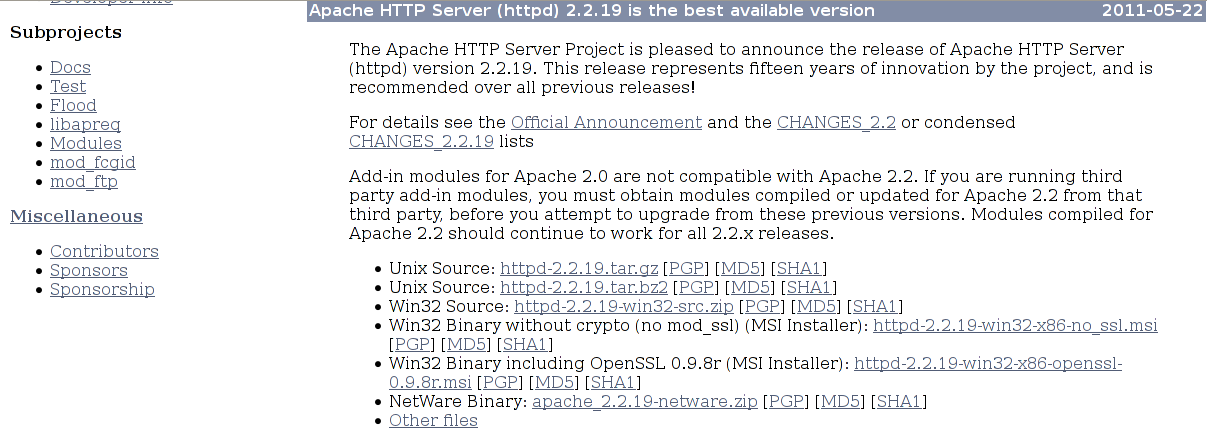
\includegraphics[width=400bp]{cap01/Screenshot.png}
  \caption{Pagina oficială Apache HTTPD}
  \label{fig:httpd homepage}
\end{figure}


Alege un \textsl{mirror}\footnote{
Un mirror este o oglindire a unor fişiere. Mai multe firme sau instituţii au ales
să pună la dispoziţie oglindiri ale fişierelor de instalare pentru apache. Oricine
poate face un mirror, însă e recomandat să înştiinţezi autorul oficial, pentru
ca acesta să pună un link către mirror-ul tău. Toate fişierele de pe un mirror sunt identice,
deci teoretic nu contează ce mirror alegi, însă este recomandat să alegi un mirror
apropiat ţie din punct de vedere geografic, pentru ca descărcarea să fie mai
rapidă.} şi apasă \texttt{change}. Mirror-ul selectat automat ar trebui să fie unul
dintre cele mai bune. Apoi selectează versiunea {\glqq}Win32 Binary without crypto{\grqq}.

%\begin{figure}[ht!]
%  \centering
%    \includegraphics[width=400bp]{cap01/Screenshot-1.png}
%  \caption{Setarea iniţială apache httpd}
%  \label{fig:httpd setup}
%\end{figure}

Introdu datele ca în figura \ref{fig:httpd setup} şi treci la pasul următor.

\begin{figure}[ht!]
  \centering
    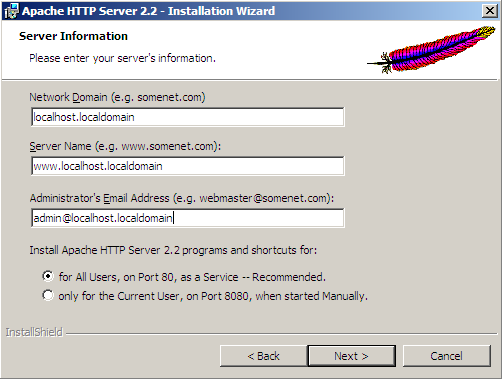
\includegraphics[width=300bp]{cap01/Screenshot-2.png}
  \caption{Setarea iniţială apache httpd}
  \label{fig:httpd setup}
\end{figure}

Alege modul de instalare \texttt{custom}, deoarece vrem să decidem exact unde şi ce
se instalează, ca în \ref{fig:httpd check custom setup}.

\begin{figure}[ht!]
  \centering
    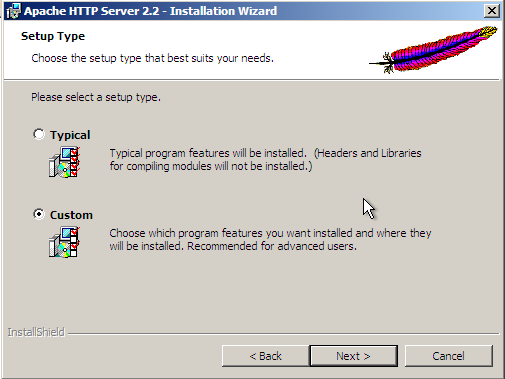
\includegraphics[width=250bp]{cap01/Screenshot-3.png}
  \caption{Setare personalizată}
  \label{fig:httpd check custom setup}
\end{figure}

În figura \ref{fig:httpd components tree} avem un arbore cu toate componentele instalate. \texttt{Apache HTTP Server 2.2.14}
este părintele tuturor componentelor. Selectează-l şi apasă pe butonul
\texttt{Change...} pentru a schimba locul de instalare.

\begin{figure}[ht!]
  \centering
    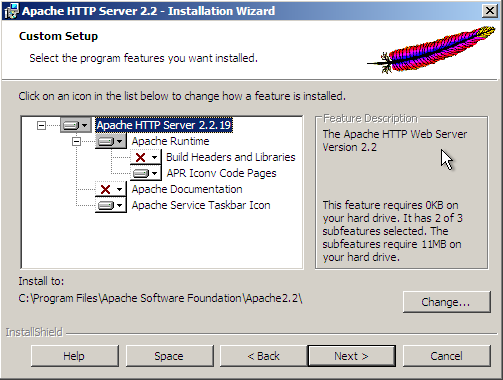
\includegraphics[width=248bp]{cap01/Screenshot-4.png}
  \caption{Setare httpd - Componentele instalate}
  \label{fig:httpd components tree}
\end{figure}

Crează un nou director \texttt{C:{\textbackslash}webdev\textbackslash}
unde vor fi instalate toate sculele
de programare web, introducând manual calea \texttt{C:{\textbackslash}webdev{\textbackslash}apache}
exact ca în \ref{fig:httpd custom path}.

\begin{figure}[ht!]
  \centering
    \includegraphics[width=253bp]{cap01/Screenshot-5.png}
  \caption{Setare httpd - Calea instalării}
  \label{fig:httpd custom path}
\end{figure}

Confirmarea te va aduce la dialogul anterior, iar în partea de jos ar trebui să scrie
că programul va fi instalat la acea locaţie.

Finalizează instalarea. La vizitarea adresei \url{http://localhost/} ar trebui să
vezi mesajul \texttt{It works!}. Asta înseamnă că daemonul apache este setat corect şi poate deservi
pagini statice în formatul html, iar calculatorul tău este acum un server.

Noi însă vrem să generăm în mod dinamic cod HTML cu PHP. Deci intră pe pagina oficială
PHP\footnote{\url{http://php.net}} şi urmează linkul de download,
sub \texttt{Windows binaries}\footnote{În părţile ce urmează se foloseşte
versiunea 5.3.6, dar tu trebuie să alegi ultima versiune stabilă. Important este 
doar să selectezi versiunea compilată cu VC9, care este thread-safe.}.
Selectează tipul de executabil \texttt{VC9 x86 Thread Safe} pentru
versiunea PHP 5.3, ca în \ref{fig:php build type}, apoi
descarcă arhiva .zip care conţine PHP, salvând-o în \texttt{C:{\textbackslash}webdev\textbackslash}.
\begin{figure}[ht!]
  \centering
    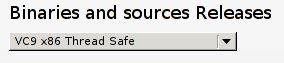
\includegraphics[width=150bp]{cap01/Screenshot-7.png}
  \caption{PHP - Tipul \textsl{build}-ului PHP}
  \label{fig:php build type}
\end{figure}


%\begin{center}
%\includegraphics[width=200bp]{cap01/Screenshot-8.png}
%\end{center}

După dezarhivare, conţinutul său va arăta ca în Figura \ref{fig:php what you get}.

\begin{figure}[ht!]
  \centering
    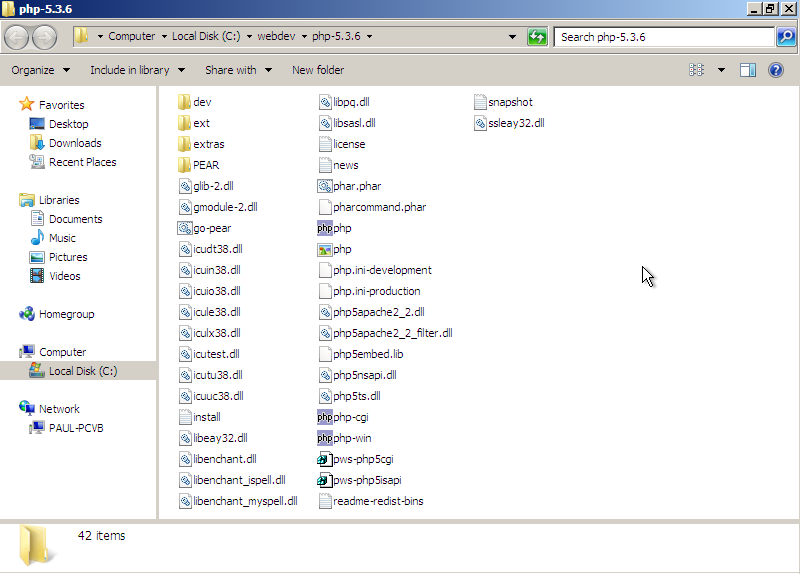
\includegraphics[width=200bp]{cap01/Screenshot-9.png}
  \caption{PHP - What you get}
  \label{fig:php what you get}
\end{figure}

Înainte de a trece la integrarea lui PHP în apache, îţi recomand să
instalezi un editor text ideal pentru începătorii în programare:
\href{http://notepad-plus.sourceforge.net/}{Notepad++}
\footnote{\url{http://notepad-plus.sourceforge.net/}}, de pe pagina oficială.
%\begin{center}
%\includegraphics[width=320bp]{cap01/Screenshot-10.png}
%\end{center}
%
%Descarcă programul de instalare şi instalează notepad++:
%\begin{center}
%\includegraphics[width=350bp]{cap01/Screenshot-11.png}
%\end{center}

\attention{Notepad++ este foarte bun ca editor deoarece, fiind un editor text,
vezi exact ce faci, preluând controlul, aşa cum ar trebui să o facă
orice programator. Pe lângă asta, Notepad++ îţi şi colorează textul
dacă recunoaşte limbajul în care scrii acel text, precum PHP sau HTML.}

\bad{Dacă eşti cumva tentat să foloseşti editoare WYSIWYG\footnote{what
you see is what you get} precum Dreamweaver, atunci ar trebui să
te opreşti acum - programarea nu e pentru tine. De ce? În afară
de faptul că un astfel de editor nu te-ar stimula să înveţi, ţi-ar
şi crea mai multe probleme. Cu PHP, tu ca programator vei prelua
controlul şi vei genera HTML. Pe lânga asta, astfel de programe
nu sunt destul de puternice ca o minte umană, şi mai şi generează
cod greşit.}
\footnotetext{\href{http://en.wikipedia.org/wiki/WYSIWYG}{what you see is what you get}}

PHP poate fi folosit şi ca limbaj de scripting general, nu doar pentru
generarea dinamică de HTML. Însă pentru asta trebuie setată calea
către directorul php care conţine fişierul de configurare \texttt{php.ini},
asupra căruia voi reveni puţin mai târziu.

Sub Windows XP, click dreapta pe \texttt{My Computer} şi apoi \texttt{Properties}.
Sub Windows 7, în \texttt{start} -> \texttt{run} introdu comanda:

\texttt{C:{\textbackslash}Windows{\textbackslash}System32{\textbackslash}SystemPropertiesAdvanced.exe}

Alege tabul \texttt{Advanced}, apoi click pe \texttt{Environment Variables} în partea de jos
a dialogului, aşa cum vezi în Figura \ref{fig:win adv props}.
\begin{figure}[ht!]
  \centering
    \includegraphics[width=200bp]{cap01/Screenshot-12.png}
  \caption{Proprietăţile avansate ale sistemului Windows XP}
  \label{fig:win adv props}
\end{figure}

Se va deschide un dialog similar cu cel din Figura \ref{img:win env vars}.
\begin{figure}[ht!]
  \centering
    \includegraphics[width=180bp]{cap01/Screenshot-13.png}
  \caption{Variabilele de mediu ale unui sistem Windows}
  \label{img:win env vars}
\end{figure}

Click pe \texttt{New} sub \texttt{System variables}, şi introdu datele ca în
Figura \ref{img:win new env var}. Această nouă variabilă de mediu
îl va ajuta pe PHP să-şi găsească fişierul de configurare \texttt{php.ini}.
\begin{figure}[ht!]
  \centering
    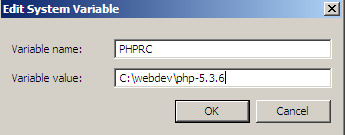
\includegraphics[width=180bp]{cap01/Screenshot-14.png}
  \caption{Variabilele de mediu ale unui sistem Windows}
  \label{img:win new env var}
\end{figure}

În acest moment, PHP este setat şi l-am putea lansa în execuţie folosind
calea absolută
\texttt{C:{\textbackslash}webdev{\textbackslash}php-5.3.6{\textbackslash}php.exe}, ceea ce
poate deveni obositor cu timpul. Însă putem integra \texttt{php.exe}
în sistem astfel încât să fie recunoscut ca comandă.

Pentru ca asta să
se întâmple, identifică
variabila systemului numită \texttt{Path}
%\begin{figure}[ht!]
%  \centering
%    \includegraphics[width=180bp]{cap01/Screenshot-20.png}
%  \caption{Variabila de mediu PATH}
%  \label{img:win env path}
%\end{figure}
şi adaugă-i la sfârşit:
\texttt{;C:{\textbackslash}webdev{\textbackslash}php-5.3.6{\textbackslash}}, ca în
Figura \ref{img:win env path}.
\begin{figure}[ht!]
  \centering
    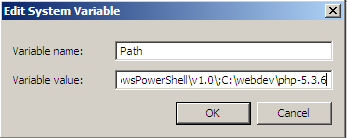
\includegraphics[width=180bp]{cap01/Screenshot-21.png}
  \caption{Variabila de mediu PATH}
  \label{img:win env path}
\end{figure}

\attention{Acel ';' de la început este foarte important. \texttt{PATH}
conţine o listă de directoare în care windows se va uita pe rând atunci
când lansezi în execuţie un program ca pe o comandă. ';' are rolul
de a separa aceste directoare.}

Un singur lucru mai lipseşte: \texttt{php.ini}. Arhiva pe care tocmai
ai descărcat-o vine cu două astfel de fişiere, \texttt{php.ini-development} şi
\texttt{php.ini-production}. Fă o \textit{copie} a fişierului
\texttt{php.ini-development} şi redenumeşte-o \texttt{php.ini}.

Testează dacă ai setat totul cum trebuie deschizând o nouă instanţă
a promptului ms-dos.
Acolo introdu comanda \texttt{php -{}-ini}.
Totul este corect dacă php este găsit de sistem, iar comanda de mai sus îţi
arată \texttt{C:{\textbackslash}webdev{\textbackslash}php-5.3.6{\textbackslash}php.ini}
ca \textit{Loaded Configuration File}.

%Mai multe informaţii despre PHP ca limbaj de scripting CLI găseşti pe
%\url{http://www.php-cli.com/}.

\vspace{1em}

Acum vom trece la integrarea lui PHP ca modul apache. Vom spune că folosim
\engl{SAPI-ul\footnote{\url{http://en.wikipedia.org/wiki/Server_Application_Programming_Interface}}}{server application programming interface}
apache2. În directorul în care ai instalat apache este un subdirector de configurare
numit sugestiv \texttt{conf/}, unde rezidă toate fişierele de configurare
pentru apache.

Fişierul principal de configurare  al apache se numeşte \texttt{httpd.conf}. Este singurul
fişier încărcat automat de apache pentru a citi configuraţia, celelalte fişiere
trebuie incluse folosind directiva \texttt{Include} din acest fişier
principal (en. \textsl{the master configuration file}). Liniile care încep
cu caracterul diez (\#) sunt comentarii, iar conţinutul lor nu este luat
în considerare, chiar dacă conţine directive de configurare valide.

Deschide \texttt{httpd.conf} cu notepad++ şi adaugă-i la sfârşit
(combinaţia \keystroke{CTRL+END}) directiva
\texttt{Include conf/extra/httpd-php.conf}
apoi crează un nou fişier cu \keystroke{CTRL+N} cu acest conţinut:
\begin{verbatim}
LoadModule php5_module "C:/webdev/php-5.3.6/php5apache2_2.dll"
AddType application/x-httpd-php .php
PHPIniDir "C:/webdev/php-5.3.6"

<IfModule dir_module>
    DirectoryIndex index.php index.html
</IfModule>
\end{verbatim}

Acum apasă \keystroke{CTRL+S} şi salvează-l ca \texttt{httpd-php.conf}
în directorul
C:\texttt{{\textbackslash}webdev{\textbackslash}apache{\textbackslash}conf{\textbackslash}extra{\textbackslash}}

Directiva \texttt{LoadModule} îi spune să încarce un fişier ca modul apache. \texttt{AddType}
îl instruieşte să interpreteze fişiere ce se termină în .php ca 
\texttt{application/x-httpd-php}, care este un tip 
\engl{MIME\footnote{\url{http://en.wikipedia.org/wiki/Multipurpose_Internet_Mail_Extensions}}}{multipurpose internet mail extension}.
\texttt{PHPIniDir} îi spune lui PHP (de data asta modulului PHP) unde îşi găseşte fişierul
de configurare \texttt{php.ini}, aşa cum variabila de mediu \texttt{PHPRC} pe care
am setat-o anterior îi spune acelaşi lucru SAPI-ului CLI (adică lui \texttt{php.exe}).

Acel bloc condiţional\footnote{Se numeşte condiţional deoarece ceea ce se află
în interiorul său este inclus doar dacă condiţia este adevărată, numele însuşi
conţinând \texttt{If}.}
 \texttt{IfModule} verifică dacă apache are modulul {\glqq}dir{\grqq}, şi dacă
da, setează resursa de start corespunzătoare root-ului (atunci când este accesat {\glqq}/{\grqq}
al unui director, aşa cum ai văzut în capitolul anterior) fiecărui director. Fişierele
sunt listate după ordinea priorităţii, dacă primul nu este găsit, apache va încerca să-l
deservească pe al doilea.

\attention{O altă directivă importantă din \texttt{httpd.conf} este
\texttt{DocumentRoot}. Acesta îi spune lui apache de unde
să deservească fişiere. În mod standard, acest director se numeşte
\texttt{htdocs} -- \textsl{hypertext documents}.}

Acum că avem totul setat, restartează daemonul httpd, în caz că e pornit, pentru a prelua
toate schimbările din \texttt{httpd.conf} şi fişierele incluse de acesta. Ar fi trebuit să-i
dăm restart şi dacă am fi modificat configuraţia php din \texttt{php.ini}.

Pentru a verifica instalarea şi configurarea lui PHP ca modul apache, crează un nou fişier
şi salvează-l ca 
\texttt{C:{\textbackslash}webdev{\textbackslash}apache{\textbackslash}htdocs{\textbackslash}info.php}
. Apoi introdu următorul text, numit şi cod sursă (în limbajul PHP):
\lstinputlisting[caption={phpinfo() furnizează toate informaţiile despre instalarea PHP curentă}]{cap01/info.php}
şi salvează-l. 

Acum intră pe adresa \url{http://localhost/info.php}. Ar trebui să vezi ceva similar cu Figura \ref{img:php phpinfo}.

\begin{figure}[ht!]
  \centering
    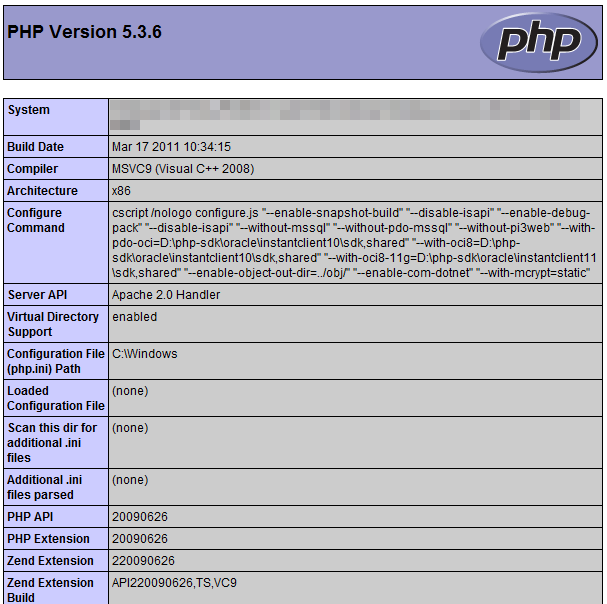
\includegraphics[width=300bp]{cap01/Screenshot-15.png}
  \caption{Informaţii afişate de un apel la phpinfo()}
  \label{img:php phpinfo}
\end{figure}

Felicitări, acum ai PHP instalat şi poţi învăţa programare, fie folosindu-l pentru programare web
ca modul apache, fie folosindu-l ca limbaj de scripting universal folosind SAPI-ul CLI (programul \texttt{php.exe}).

SAPI-urile există tocmai pentru a uşura integrarea lui PHP în toate aceste medii: pentru web putem folosi
un SAPI specific daemonului folosit, de exemplu pentru apache avem SAPI-ul php5apache2\_2.dll.
Acest fişier DLL reprezintă însă doar interfaţa (SAPI-ul, aşa cum îi spune şi numele de \textsl{interface})
de comunicare dintre apache şi "adevăratul PHP".

Pe acelaşi calapod, \texttt{php.exe} reprezintă interfaţa de comunicare dintre promptul ms-dos
(sau shell, într-un sistem *NIX) şi acelaşi "adevărat PHP" ca şi în cazul apache. Altfel spus,
ambele, atât \texttt{php.exe}, cât şi \texttt{php5apache2\_2.dll} sunt două SAPI-uri,
fiecare destinate integrării lui PHP în mediile lor specifice de execuţie a scripturilor PHP.

În capitolul următor ne vom uita mai îndeaproape la limbajul PHP.


%variabile, controlul fluxului de executie, input formulare GET
\chapter[Controlul fluxului de execuție și de date]{Controlul
fluxului de execuție\footnote{en.
\textsl{execution flow}} și de date\footnote{en.
\textsl{data flow}}}
\vskip -25pt
\textit{Înțelegerea fluxului de execuție este primordială
în crearea de aplicații care fac mai mult decât simple
afișări -- care iau decizii și îți fac \textsl{site}-ul dinamic.
Indiferent de cât de simplă sau cât de complexă va fi aplicația ta,
indiferent dacă vei folosi baze de date sau simple fișiere,
cu siguranță vei folosi fluxul de execuție pentru a controla
fluxul de date. Acest capitol te introduce în lumea datelor,
iar apoi îți arată cum să le manipulezi.
}

\vskip 5em



\chapter[Controlul fluxului de execuție și de date]{Controlul
fluxului de execuție\footnote{en.
\textsl{execution flow}} și de date\footnote{en.
\textsl{data flow}}}

\begin{chapsummary}
Înțelegerea fluxului de execuție este primordială
în crearea de aplicații care fac mai mult decât simple
afișări -- care iau decizii și îți fac \textsl{site}-ul dinamic.
Indiferent de cât de simplă sau cât de complexă va fi aplicația ta,
indiferent dacă vei folosi baze de date sau simple fișiere,
cu siguranță vei folosi fluxul de execuție pentru a controla
fluxul de date. Acest capitol te introduce în lumea datelor,
iar apoi îți arată cum să le manipulezi.
\end{chapsummary}

\section{O altfel de reîmprospătare}
%\linenumbers

Vreau să stabilesc niște lucruri care probabil nu sunt evidente
pentru tine, sau asupra cărora nu ai insistat prea mult
când ai început să înveți să creezi \textit{site}-uri statice
cu HTML, eventual cu CSS sau poate chiar cu interacțiune
în interiorul browserului cu JavaScript.

HTML este un \engl{limbaj de formatare}{markup language}.
Cu el nu controlezi ceva, nu iei decizii, deci nu este
un limbaj de programare. În HTML doar
structurezi un document. În mod ideal îl structurezi
semantic (\href{http://en.wikipedia.org/wiki/Semantic_HTML}{semantic HTML}),
pentru a putea fi interpretat mai bine de motoarele de căutare web
(en. \textsl{search engine}).

Există multe formate de fișiere, și chiar în capitolul anterior ai
lucrat cu două astfel de formate -- formatul de configurare specific apache, și protocolul
HTTP. Dacă îți amintești,
ți-am explicat pe rând ce înseamnă directive precum \texttt{Include}.
Semnificația acestor directive, sau general spus, semnificația oricărei
entități specifice unui limbaj (fie el de markup -- HTML, de configurare
-- \texttt{httpd.conf}, de programare -- PHP, sau un protocol de
comunicare -- HTTP) constituie \textsl{semantica}
acelui limbaj.

Semantica unui anumit construct al unui limbaj (de orice natură
ar fi el) este strâns legată de \textit{contextul} în care se află acel
construct.
De exemplu, pentru a cere o resursă cu HTTP, am văzut că
poți începe cererea cu GET, urmat
de o cale absolută (care începe cu ``/'') din cadrul \texttt{Host}-ului
în cauză. Calea respectivă are semnificația pe care o vrem
doar în contextul lui ``GET'', ca dovadă că atunci când vedem
căi de genul \texttt{/script.php} pe site-uri web,
acestea nu sunt interpretate automat ca parametri GET, și
deci browserul nostru nu este redirecționat către acele pagini.

\textsl{Contextul} a ceva înseamnă în ce punem acel ceva pentru a
avea o anumită semantică. De exemplu, sarea pusă în contextul
gătitului are semantica de \textit{condiment}, dar dacă
o pui pe o rană, are semantica de \textit{ceva care provoacă durere}.
Cu alte cuvinte, \textsl{context} înseamnă
\textsl{circumstanțe} sau \textsl{mediul înconjurător}. 

Analog, ``HTTP/1.1'' are semantica de ``protocolul și versiunea folosită''
în contextul \textit{request line}-ului HTTP al unui \textit{request HTTP}.

\begin{Exercise}[title={Întrebări de sinteză},difficulty=2]
Însă și GET însuși are semnificația pe care ai întâlnit-o în capitolul
trecut doar într-un anumit context semantic.

\Question Care este acest context semantic?
\Question În ce context semantic are semantica întâlnită constructul \texttt{Include}?
\Question În ce context semantic are sens comunicarea în limbajul (în protocolul) HTTP?
\ExeText Determină contextul semantic în care următoarele constructe au semantica pe
care o intuiești ca cunoscător al limbajului HTML:
\Question <td>
\Question <tr>
\Question <body>
\Question <html>
\Question href
\end{Exercise}


\attention{Dacă ai avut dificultăți majore la
răspunderea întrebărilor de sinteză, te rog ia atitudine. În primul
rând, plec de la premiza că citești cu atenție, și că reții tot
ce-ți povestesc. Toate noțiunile pe care le introduc, le introduc
pentru că astfel voi putea explica lucruri destul de complicate
mai târziu, pe baza celor spuse aici. \textit{Asta îți va permite să
știi multe învățând cât mai puțin}. ``Dezavantajul'' este că
va trebui să fii concentrat la ce citești, și să sintetizezi
singur mult. Sinteza aceasta este un exercițiu perfect pentru
tine ca viitor programator, deoarece atunci când vei programa
vei fi confruntat cu această nevoie de a sintetiza lucruri.
Metoda mea de predare, deși dură, te pregătește foarte bine pentru
cariera ta de programator. Deci dacă simți că nu ești stăpân
pe ce ai învățat până acum despre rețelistică
și despre semantică, recitește acum, până nu te pierzi definitiv.
Când recitești, urmează link-urile menționate -- după cum am spus
în capitolul Introducere, acestea nu sunt lectură opțională.}

Pe lângă semantică, un limbaj mai are și o \textsl{sintaxă}. Regulile sintactice
ale limbajelor sunt necesare pentru a crea contextul semantic în
care vor exista constructele acelui limbaj.

Vreau să ilustrez asta cu un exemplu: în protocolul HTTP, GET trebuie
să fie separat de cale printr-un spațiu. Asta este o regulă sintactică
a limbajului, standardizată prin
RFC-uri,
însă practic separatorul ar putea fi orice altceva.
Însă un separator trebuie să fie acolo, altfel calculatorul (browser-ul
sau daemon-ul) nu ar putea decide unde începe cuvântul cheie ``GET'', unde
se termină, și unde începe calea către resursa pe care o dorim.
Aceste reguli sintactice
permit programelor precum daemon-uri și clienți HTTP
să parseze (să ``înțeleagă'') datele comunicate reciproc.

Există multe posibilități de a exprima sintaxa unui limbaj, însă acestea
sunt mult prea complexe pentru noi. Însă există un standard nescris
pentru a specifica sintaxa unor constructe simple, într-o singură linie.
Ea se leagă de necesitatea unui anumit parametru.

De exemplu, sintaxa constructului GET ar putea fi:\\
\begin{verbatim}'GET ' <RESOURCE> ' HTTP/1.1'\end{verbatim}
\texttt{RESOURCE} este pus între < și >, ceea ce denotă că
este un parametru necesar, care trebuie specificat.
'GET ' (inclusiv spațiul) și ' HTTP/1.1' sunt puse
între apostrofuri pentru a arăta că sunt lucruri
ce trebuie scrise exact așa cum sunt. \texttt{RESOURCE}
este numele simbolic al parametrului, pe care îl putem
refolosi în documentația limbajului (în cazul nostru,
documentarea limbajului HTTP, sau mai bine spus, a unei
cereri HTTP de bază).

Pentru a specifica că un parametru e opțional, îl punem între [ și ].
Astfel, sintaxa unei cereri HTTP ca cea pe care am făcut-o în capitolul
anterior, împreună cu descrierea ei, ar putea arăta astfel:
\begin{verbatim}
'GET ' <resource> ' HTTP/' <version> <enter>
['Host: ' <name enter> ]<enter>

	- resource	= the absolute path to the resource
	- version 	= the version of the HTTP protocol used;
             currently only 1.0 and 1.1 are supported
	- name	    = the hostname
	- enter    = press return once
\end{verbatim}

Pe lângă lucrurile evidente pe care ni le spune această specificație
sintactică, ne mai spune și un lucru care probabil ți-a scăpat:
câmpul \texttt{Host} este opțional, dar dacă îl specificăm, atunci
trebuie să specificăm și parametrul \texttt{name}, și să și apăsăm o dată enter.

Cu siguranță ai realizat că astfel de reguli pot fi incluse una în alta,
creând reguli destul de complexe.

Un limbaj precum cel de mai sus, care folosește <,>,[,] pentru a specifica
un alt limbaj se numește un \textsl{metalimbaj}. \textit{Meta} înseamnă
\textit{care descrie} - \textit{un limbaj care descrie limbajul}.



Cel mai probabil ai întâlnit deja \textsl{tag}-ul HTML \texttt{<meta>}, de aici
îi provine numele. Diferența este că \texttt{<meta>} nu se referă la limbaj (HTML
în cazul de față), ci la informații. Ceea ce \texttt{<meta>} ne spune despre
documentul HTML în care se află se numesc \textsl{metainformații} - \textit{informații
care descriu informațiile din documentul curent}.

Probabil ai folosit deja un forum pe web. Probabil că acel forum
îți spunea la un moment dat că autorul unei intrări (al unui \textsl{topic}
sau \textsl{thread}) se numește Xulescu. Ei bine, în timp ce
intrarea propriu-zisă constituie informația, numele autorului
este o \engl{metainformație}{metadata} - o informație despre
informație.
%Vom reveni mai târziu asupra conceptului de metainformație.

\attention{
La ce îți folosește această cunoaștere despre metadate, metalimbaje, sintaxă
și semantică? În primul rând, ai învățat primul cel mai important
lucru pragmatic din viitoarea ta carieră de programator: să citești manualul
(PHP sau orice altceva) -- chiar dacă încă
nu ești conștient de asta.

\smallskip

În al doilea rând, meta-ceva-urile te vor însoți
în toate aplicațiile pe care le vei programa. Uită-te
la toate aplicațiile pe care le folosești, vei vedea
că toate au niște metadate. Singurul lucru care
te-ar împiedica să vezi asta este că datele și
metadatele se întretaie atât de mult încât e
greu să le identifici pe fiecare.

\smallskip

Și în al treilea rând, pentru a te pregăti pentru
exercițiile următoare care au menirea de a te dezgheța la minte puțin,
deoarece, din păcate, nu știu nimic despre cititorul meu, însă trebuie
să mă asigur cumva că este pe aceeași lungime de undă ca mine, ceea ce-i
permite să asimileze cât mai eficient cunoașterea prezentată
în continuare, fără risipă de cuvinte.}

%TODO spune că e un pattern, că 'aba' este potrivit de X Y X, deoarece respectă 'modelul'


\begin{Exercise}[title={Reguli sintactice},difficulty=1]
Fie regula sintactică
%TODO corectează 'A' 'B' 'C'
\begin{verbatim}
                 [A] A [A A] [A [A <B>]] <C>
\end{verbatim}
\ExePart
Care dintre următoarele inputuri o respectă?
\Question AABC % nu
\Question AAAAC % da
\Question AC % da
\Question AAAC % da
\Question AAABC % da
\ExePart
Detașează-te de nivelul abstract al acestei reguli sintactice, și fă o afirmație
\textit{pragmatică} despre B. Afirmația începe așa:
\textit{Într-un input valid, B este mereu \ldots} % este mereu precedat de cel putin 3, de maxim 6 A-uri
\end{Exercise}

Metalimbajul prezentat nu este bătut în cuie. În primul rând,
caracterele speciale ale limbajului <,>,[,] și ' pot fi schimbate
în orice, atâta timp cât documentezi aceste schimbări aduse de tine.

Deasemenea, nu este decât un standard nescris, și îl poți
extinde în ce fel ai nevoie. Din nou, important este doar
să documentezi ``extensiile'' aduse metalimbajului astfel
încât ceilalți programatori să îți înțeleagă specificația
limbajului pe care îl descrii cu ajutorul acelei
extensii proprii a metalimbajului.

De exemplu, să zicem că vrem să introducem un nou
construct în acest metalimbaj care să însemne \textit{simbolul
din stânga mea poate apărea o dată sau de mai multe ori}, și
ne decidem să folosim simbolul '+' pentru asta.

Astfel o regulă de genul:
\begin{verbatim}
	<FOO+> [BAR+]
\end{verbatim}
S-ar putea citi ca: \textit{Unul sau mai mulți \texttt{FOO} urmat de zero sau mai
mulți \texttt{BAR}}. Un astfel de simbol precum '+' se numește \textsl{cuantificator}.
Ar fi la îndemână să stabilim, în documentația extensiei noastre adusă metalimbajului,
că '+' poate cuantifica orice entitate din stânga sa, inclusiv o grupare <> sau [].

Documentația ar suna așa:
\begin{verbatim}
+ = repeat the entity on its left once or multiple times (a quantifier)
    the entity can be any SYMBOL, <required parameter> or
	[optional parameter]
\end{verbatim}
Iar exemplul de mai sus, în care vrem ca \texttt{FOO} și \texttt{BAR}
să fie separați de un eventual spațiu, ar deveni:
\begin{verbatim}
	<FOO ' '>+ [BAR ' ']+
\end{verbatim}

Până acum definițiile noastre sintactice se limitau doar la
o singură regulă (o singură linie), însă am putea introduce
constructe în metalimbaj care ne-ar da voie să atribuim nume
acestor reguli, și să refolosim acele nume în definițiile altor
reguli sintactice, creând astfel interdependențe între reguli,
și deci crea specificațiile unor limbaje foarte complexe.

\attention{Majoritatea limbajelor de programare, inclusiv
PHP, sunt definite în astfel de limbaje.}

\begin{Exercise}[title={Sintaxa HTML},label={ex:sintaxa_html},difficulty=3]
Acum hai să aplicăm ce am învățat asupra limbajului HTML. În HTML avem
tag-uri (ex. \texttt{<html>}) care au atribute și valori.

\Question Crează o specificație sintactică a limbajului HTML folosind
doar cuvintele cheie TAG, ATTRIBUTE și VALUE, care combinate
cu [] și <> să reflecte cât mai corect sintaxa limbajului.

Specificația trebuie să valideze orice text HTML valid.
Un exemplu de input ar fi:
\begin{verbatim}
<form method="get">
   <checkbox name="hello" checked>
   <input type="submit">
</form>
\end{verbatim}
\ExeText
Note:
\begin{itemize}
\item Regula creată \textit{nu} trebuie să ia în calcul sintaxa
specifică XHTML (în care de exemplu '<img>' ar fi greșit, doar '<img />' este valid).
\item Se pleacă de la premiza că inputul este cel mai curat HTML posibil, că
sunt folosite " pentru a delimita valorile atributelor (dacă acestea există), că
nu e mai mult de un spațiu acolo unde e nevoie de spațiu, ș.a.m.d. Pe scurt:
folosește-ți intuiția pentru a decide ce înseamnă ``cel mai curat HTML posibil''.
\item Deoarece caracterele < și > au o semnificație specială în limbajul HTML, pe
care încerci să-l descrii sintactic folosind printre altele
și caracterele < și > înseși, va trebui să le pui între apostrofuri, pentru a face
diferența între <,> care ne spun în metalimbajul nostru
că acel parametru este necesar, și '<' sau '>' care
ne spun că ne referim la caracterul '<' respectiv '>' în limbajul pe care
vrem să-l descriem (adică HTML însuși).
\item Va trebui să extinzi metalimbajul (nu uita să și documentezi extensiile aduse)
pentru a ajunge la o rezolvare cât mai corectă și completă
\item Exercițiul este destul de dificil. Încearcă să te apropii cât mai mult de soluția
cea mai corectă și completă.
\end{itemize}
\end{Exercise}

\section{Output simplu}
\label{sec:output simplu}
La sfârșitul capitolului anterior, ai făcut cunoștință
cu primul tău cod PHP:
\lstinputlisting{cap01/info.php}

Prima linie marchează începutul procesării PHP. Ce se află
înaintea \texttt{<?php} este trimis așa cum este către client.
Hai să testăm. Scrie ceva în tagul <h1> înainte de începutul
procesării PHP și vezi ce iese:
\lstinputlisting{cap02/1-helloinfo.php}

PHP generează prea mult cod HTML pentru gusturile noastre simpliste, deci
fă cunoștință cu un cuvânt cheie în PHP: \texttt{echo}. Sintaxa
generală este:
\begin{verbatim}
echo <EXPR>;
\end{verbatim}
unde \texttt{EXPR}  trebuie să fie o expresie care evaluată, se reduce la o valoare.

\attention{Nu te speria dacă nu înțelegi totul, voi reveni asupra subiectului. Deocamdată urmează pur și simplu pașii prezentați de mine, respectând sintaxa.
Simte-te liber să faci modificări, să experimentezi. Dacă faci ceva ce generează
o avertizare sau o eroare nu te impacienta, citește-o cu atenție, încearcă
să o înțelegi, și cere lămuriri pe wiki-ul proiectului.
}

Hai să-l învățăm pe PHP să ne salute. În notepad++ crează un nou fișier
și salvează-l ca \texttt{salut.php} în htdocs, apoi introdu codul:
\begin{lstlisting}
<?php
echo 'Salut Flavius';
\end{lstlisting}
Acum fă cu telnet o cerere HTTP, să vezi exact ce se întâmplă atunci când
interpreterul PHP execută acel cod:
\begin{verbatim}
GET /salut.php HTTP/1.1
Host: localhost
\end{verbatim}

Ce observăm? Exact! Observăm că nu vedem nici urmă de cod PHP, vedem doar
outputul generat de el. Nu tu \texttt{<?php}, nu tu \texttt{echo}. Asta
ne demonstrează că PHP ne-a procesat scriptul, script care a generat
output. Dacă scriptul nu ar fi generat output, \textit{response body}-ul
HTTP ar fi fost gol.

În al doilea rând, \textsl{http response body} nu conține date în format HTML.
De ce? Simplu, deoarece nu i-ai spus niciunde să genereze nimic ce ar putea arăta a
HTML. Cum facem asta? O posibilitate ar fi următoarea:
\begin{lstlisting}
<?php
echo '<html><body>';
echo 'Salut Flavius';
echo '</body></html>';
\end{lstlisting}

Concluzia pe care o tragem este că PHP habar n-are ce este HTML. De ce?
După cum am spus atunci când ai instalat CLI-ul PHP (numit \texttt{php.exe}),
PHP este un limbaj de scripting general. De fapt nu este legat în niciun mod de
HTML sau de site-uri. Este doar felul în care îl folosim noi și majoritatea
restului lumii. De fapt, PHP poate genera orice, imagini, documente, animații
(flash). Chiar nu ești restrâns la HTML, dar nici nu te ajută în acest sens --
trebuie să scrii manual codul HTML, după cum ai văzut mai sus.

Vei vedea însă că îți pune la dispoziție constructe care înlesnesc generarea
de HTML -- de exemplu poți genera o galerie de imagini aflate într-un anumit
director pe server, fără să trebuiască să știi dinainte numele fișierelor.

Totuși exemplul nostru anterior nu prea are sens -- nu este nimic dinamic în el.
L-am putea rescrie la fel de bine doar în HTML static, însă deoarece
vreau să demonstrez altceva, voi genera totuși mesajul de salut cu PHP:
\begin{lstlisting}
<html>
	<body>
		<?php
		echo 'Salut Flavius';
		?>
	</body>
</html>
\end{lstlisting}

Observi că pentru a termina procesarea PHP și a afișa din nou totul
așa cum este (en. \textsl{unparsed}) se folosește \texttt{?>}.
În acest mod poți porni și opri procesarea PHP de oricâte ori dorești în același fișier.
La sfârșitul fișierului procesarea este terminată automat, de aceea în exemplele
anterioare nu a fost nevoie de {\glqq}?>{\grqq}.

\attention{Mai observă și cum mi-am făcut codul ușor de citit \textsl{indent}ându-l (en.
\textsl{to indent}), adică am aliniat deschiderea fiecărui tag HTML cu tag-ul
de închidere corespunzător, făcându-mi codul lizibil. Pentru codul nostru sursă
minuscul nu prea contează, însă diferența de mentenabilitate va fi
vizibilă când fișierele vor avea sute sau mii de linii de cod (LOCs en.
\textsl{lines of code}). Deci obișnuiește-te
să indentezi codul apăsând tasta \keystroke{TAB} pentru fiecare nou nivel de
indentare necesar.}

Din acest punct înainte scopul nostru este să învățăm PHP, nu să generăm
cod HTML valid, deci nu ne vom mai obosi să decorăm textul generat
cu \texttt{html} sau \texttt{body}. Însă nu uita că într-o pagină HTML
normală, validă, și asta trebuie făcut, eventual
punând și un
\textsl{doctype}\footnote{
\href{http://en.wikipedia.org/wiki/Document_Type_Declaration}{document type declaration}}, altfel
browserul intră în \href{http://en.wikipedia.org/wiki/Quirks_mode}{quirks mode}.

%----------------------------------------------------------
\section{Folosirea variabilelor}
Înainte de a trece la noțiuni noi, trebuie să revenim asupra exemplului nostru
cu câteva completări:
\begin{lstlisting}
<?php
echo 'Salut Flavius';
\end{lstlisting}
Știm deja că \texttt{echo} este un cuvânt cheie care generează output pe baza
primului său parametru. Sper că ai intuit deja că fiecare instrucțiune
trebuie separată de următoarea prin ';'.

Însă ce este 'Salut Flavius'? Este o valoare în primul rând, pentru că
i-o putem pasa lui \texttt{echo}. În al doilea rând, este o constantă,
deoarece nu se modifică. La fiecare interpretare a scriptului, \textit{output}-ul
va fi același. Sumarizat: este o \textsl{valoare constantă}.

Pe lângă faptul că este o valoare constantă, mai este și un \engl{șir de caractere}{string}.
Acesta este motivul pentru care
am pus mesajul între apostrofuri -- altfel PHP ar fi încercat să
interpreteze \textsl{Salut} și \textsl{Flavius} ca constructe ale limbajului,
care evident nu există.

\good{Corect terminologic spunem deci că 'Salut Flavius' este un \textit{string constant} sau
mai pe larg \textit{o valoare constantă de tip string}.}

Deci încearcă! Fă-l pe PHP să genereze erori:
\begin{lstlisting}
<?php
echo Salut Flavius;
\end{lstlisting}
Mesajul de eroare ne-ar putea părea confuz:\\
\texttt{Parse error: syntax error, unexpected T\_STRING, expecting ',' or ';'}\\
Ceea ce se întâmplă este următorul lucru: PHP citește \texttt{echo}, și deoarece a citit
și a recunoscut instrucțiunea \texttt{echo}, intră în contextul semantic în care se așteaptă ca următorul
lucru să fie o valoare, însă nu găsește una, ci întâlnește \texttt{Salut},
pe care nu-l recunoaște\footnote{De fapt, parserul se blochează la {\glqq}Flavius{\grqq}, însă
ca să explic asta cum trebuie, ar fi trebuit să fi introdus deja constantele}
ca și construct al limbajului.
De aceea ne spune că nu se așteaptă să vadă T\_STRING-ul \texttt{Salut}.

Dar stai puțin, de ce îl numește {\glqq}T\_\textbf{STRING}{\grqq}, dar nu îl acceptă ca string?
Pentru a înțelege asta, trebuie să privești puțin lucrurile din perspectiva parserului
PHP. Codul sursă pe care îl scriem în limbajul PHP este folosit ca input pentru
parser. Acest input scris de noi este citit de PHP ca string, ca un șir de caractere.
Din acest motiv PHP ne spune foarte corect că nu se așteaptă să vadă acel string acolo,
ci altceva.
\attention{Pentru PHP, codul scris de noi este un simplu text.}
Hai să vedem ce ar genera PHP dacă nu s-ar aștepta să vadă un string
din perspectiva noastră:
\begin{lstlisting}
<?php
echo 'Salut' 'Flavius';
\end{lstlisting}
ne zice \texttt{Parse error: syntax error, unexpected T\_CONSTANT\_ENCAPSED\_STRING}.

Ce înveți din asta? În primul rând, înveți că mesajele de eroare, deși nedorite,
oferă informații prețioase despre ce s-a întâmplat. Din proprie experiență
pot spune că vederea unui mesaj de eroare sau avertizare e ca o mână cerească,
reversul medaliei fiind mult mai frustrant: să nu vezi o eroare, dar codul
nici să nu funcționeze așa cum îți imaginezi că ar trebui să funcționeze -- sau
mai rău, să nu afișeze nimic, lăsându-te în întuneric complet. Deci fi fericit
când PHP îți spune ce ai greșit, caută să înțelegi ce-ți spune, și apoi
repară-ți greșeala.

Pe lângă stringuri, mai există și alte tipuri de valori constante. PHP înțelege
\engl{numere întregi}{integers}, de exemplu \texttt{42},\footnote{Sunt curios
când va veni cineva să-mi spună de ce am ales 42 :-)}
numere cu virgulă (en, \textsl{floating point numbers} sau scurt \textsl{floats}),
unde partea zecimală
e separată de partea întreagă prin punct, de ex \texttt{3.1415}, și alte lucruri
asupra cărora vom reveni. Hai să ne uităm la un exemplu:
\begin{lstlisting}
<?php
echo 'Salut 00';
echo 7;
echo '. PI este ~';
echo 3.1415;
\end{lstlisting}

\subsection{Variabile și tipuri de date elementare}
Toate bune și frumoase cu lucrurile cu care ai făcut cunoștință
până acum, însă ele nu te-au ajutat să creezi ceva dinamic.

Deci hai să facem un pas înapoi și să ne gândim ce înseamnă și
ce implică o eventuală dinamicitate. Pentru a fi dinamică, o
pagină trebuie să fie capabilă să primească date de intrare (\texttt{input}),
pentru a genera date de ieșire (\texttt{output}) pe baza acestora.

De exemplu, să zicem că vrem să facem o pagină care în loc să afișeze
mereu {\glqq}Salut Flavius{\grqq}, afișează {\glqq}Salut <nume>{\grqq}. Acest input (numele) trebuie
salvat undeva, altfel nu avem acces la el. Bine ai venit în lumea variabilelor.

O variabilă are trei caracteristici
\begin{enumerate}
\item un \textsl{nume} sau \textsl{identificator}
\item o \textsl{valoare} pe care o ține
\item \textsl{tipul de date} (en. \textsl{datatype}) al valorii\footnote{mai
spunem colocvial și \textit{tipul de date al variabilei} însă în PHP tipul
de date este inerent valorii -- vom reveni mai târziu asupra acestui aspect} precum
string, int sau float pe care le-ai cunoscut mai devreme
\end{enumerate}

Identificatorul variabilelor începe mereu cu \$, primul caracter după el
trebuie să fie o literă sau underscore (\_), iar următoarele
caractere pot fi litere, cifre, sau underscore.
Nu există o limită în lungimea identificatorului, și nici restricții privind
numirea lor. Există însă reguli nescrise pe care le vei întâlni mai târziu,
cât și variabile pe care PHP le crează automat pentru tine.

Valoarea unei variabile poate fi orice bucată de informație ce poate
fi salvată.

Tipul de date al valorii poate fi unul din cele trei prezentate mai sus,
sau altele pe care le vom cunoaște în acest capitol și în capitolele următoare.

După cum am spus, \texttt{echo} afișează valoarea unei expresii.
Această valoare poate fi una constantă, precum în exemplele anterioare,
însă poate fi și o variabilă. Exemplu:
\lstinputlisting{cap02/3-hello-var-error.php}
PHP ne va atenționa cu o notificare că am încercat să accesăm o variabilă
nedefinită. Pentru a defini o variabilă trebuie să-i atribuim o valoare
mai întâi, iar asta o facem cu \textsl{operatorul} de atribuire \textsl{=}.
Putem spune și că \textit{am salvat valoarea X în variabila Y}. Exemplu:
\lstinputlisting{cap02/4-hello-var.php}

\attention{\texttt{echo} nu adaugă automat spații niciunde. Este responsabilitatea
noastră să o facem. PHP chiar nu are noțiunea de {\glqq}cuvinte{\grqq}. Pentru el, un
șir de caractere este un șir de caractere și atât.} 

În cazul de față, variabila \texttt{\$nume} nu prea își are rostul, deoarece o
folosim o singură dată. Însă imaginează-ți că ai un script lung,
și vrei să refolosești acel nume în diferite locuri în cadrul generării de
output. Variabilele sunt ideale pentru acest lucru, deoarece nu trebuie
decât să schimbi valoarea într-un loc, iar schimbarea va fi preluată în
întregul script:
\lstinputlisting{cap02/5-hello-var-reuse.php}

Felicitări, ai creat primul tău script care reutilizează variabile.

\subsection{Operații cu string, int, float}
Cu aceste tipuri de date se pot face operații. În primul rând,
stringurile pot fi \textsl{concatenate}, indiferent dacă sunt salvate
în variabile sau provin din valori constante. A concatena
înseamnă a lipi un string de următorul, pentru a forma un nou string.
Exemple:
\lstinputlisting{cap02/6-concatenare-stringuri.php}

\textit{Linia 2} face următorul lucru: mai întâi concatenează cele două valori constante
'Salut ' și 'Flavius', operație în urma căreia rezultă \textsl{valoarea intermediară}
'Salut Flavius'. Îți poți imagina că această valoare stă acum de partea
dreaptă a operatorului de atribuire. Iar deoarece avem o atribuire, această
valoare intermediară este salvată în variabila \texttt{\$a}.

\textit{Linia 3} afișează valoarea salvată în variabila \texttt{\$a}.

Ne-am fi putut folosi de acea {\glqq}valoare intermediară{\grqq} de pe linia 2 afișand-o direct:
\begin{lstlisting}
<?php
echo 'Salut ' . 'Flavius';
\end{lstlisting}
Aici valoarea intermediară \textit{care rezultă în urma concatenării} celor două stringuri
constante este pasată direct (ca o nouă valoare) instrucțiunii \texttt{echo}.

După cum ai observat pe \textit{linia 2}, operația de atribuire este interpretată
de PHP de la dreapta la stânga. Mai întâi sunt făcute rând pe rând operațiile
din partea dreaptă a atribuirii, apoi valoarea rezultată este salvată în
variabila aflată în stânga atribuirii. Datorită acestei ordini spunem că
operația de \engl{atribuire}{assignment} este \textsl{right-associative}.

\textit{Linia 5}: Datorită asociativității de dreapta a operației de atribuire,
într-o atribuire putem folosi o variabilă precum \texttt{\$a} în partea dreaptă, genera
o valoare temporară pe care o atribuim tot variabilei \texttt{\$a}, suprascriind
valoarea sa inițială. Dacă am fi știut că mai avem nevoie de nume ca valoare
de sine stătătoare, pe linia 5 ar fi trebuit să introducem o nouă variabilă
căreia să-i atribuim noua valoare,
astfel încât să nu pierdem valoarea inițială a lui \texttt{\$a}.
Însă în cazul nostru, \textit{linia 5} este extrem de curată,
deoarece nu introduce o nouă variabilă în mod inutil.

Să revenim la sintaxă și la semantică. Sintaxa lui echo este:\\
\texttt{echo <EXPR>;}\\
Iar a operației de concatenare este:\\
\texttt{<expr1> . <expr2>}\\
<expr1> și <expr2> pot fi orice fel de expresii, fie ele valori constante,
sau variabile -- deoarece variabilele au și ele o valoare pe care
o cară cu ele. În urma operației de concatenare rezultă o valoare
intermediară. Chiar dacă aceasta e {\glqq}invizibilă{\grqq} (deoarece
PHP o crează în mod transparent pentru noi), ea este tot o valoare ca oricare
alta, deci poate fi pusă oriunde PHP ne lasă să punem o expresie.

Dar stai puțin, operația de concatenare însăși acceptă două expresii!
Consecința? Putem concatena acele valori intermediare, transparente,
într-un lanț\footnote{În matematică spunem că abordăm problema
\href{http://en.wikipedia.org/wiki/Structural_induction}{inductiv}.}:\\
\texttt{<valoare1> . <valoare2> . <valoare3> . <valoareN>}

În astfel de cazuri, <valoare1> este concatenată cu <valoare2> și rezultă
o valoare intermediară, transparentă, care este apoi concatenată cu <valoare3>,
și tot așa.
Exemplu:
\lstinputlisting{cap02/7-concatenare-stringuri.php}

Despre limbajul PHP se spune că este \textsl{dynamically typed}. Asta înseamnă
că poate (în limitele {\glqq}bunului simț{\grqq}), să convertească automat
o valoare de un tip, într-o altă valoare de alt tip, care e cât
mai apropiată de valorea inițială. Așa se face că deși operatorul
de concatenare acceptă doar doi parametri de tip string, putem totuși
concatena și numere. PHP va crea însă încă o valoare intermediară
cu reprezentarea valorii inițiale ca string. Un exemplu:
\lstinputlisting{cap02/8-concatenare-inference.php}

\attention{Încearcă să eviți a-l forța pe PHP să
trebuiască să convertească un număr într-un string,
deoarece operația asta consumă resurse inutil.
În schimb folosește sintaxa alternativă a lui \texttt{echo}
cu care vei face cunoștință în continuare.}

\begin{Exercise}[title={Primul cod propriu}]
Continuă codul următor astfel încât să afișeze\\
\texttt{Valoarea lui PI este 3.1415.}
\lstinputlisting{cap02/9-ex-pi.php}
\end{Exercise}

Există o sintaxă alternativă pentru \texttt{echo}, care ne permite
să afișăm valori constante amestecate cu valori variabile fără
a mai crea valori intermediare, deci PHP poate executa
scriptul mai rapid și cu consum mai mic de memorie.
Pentru asta punem virgulă între valori:
\lstinputlisting{cap02/10-echo-list.php}

Asta înseamnă practic că \texttt{echo} va fi apelat asupra fiecărui
parametru din listă. Atenție: diferențele se pot vedea
doar atunci când lucrezi cu cantități mari de informație.

\begin{Exercise}[difficulty=1,title={Sintaxa alternativă pentru echo}]
De câte ori va fi apelat \texttt{echo} în codul următor? % de 3 ori
\begin{lstlisting}
<?php
echo 'Salut ', 'Homer ' . 'Simpson.' , ' Ce ' . 'faci?';
\end{lstlisting}
\Question o dată
\Question de trei ori
\Question de cinci ori
\end{Exercise}

\begin{Exercise}[difficulty=2,title={Determinarea fluxului de execuție într-un exemplu simplu}]
Explică cum crezi că execută PHP următoarea linie, cât mai concret posibil, așa cum
ai văzut în explicațiile anterioare.
\lstinputlisting[label=lst:execflow echo,caption={echo'ing an assignment}]{cap02/12-ex-execflow.php}
\end{Exercise}

\subsection{Operații matematice}

PHP știe toate cele patru operații aritmetice: + pentru adunare,
- scădere, * înmulțire și / pentru împărțire. Știe și că
înmulțirea și împărțirea sunt de gradul doi, iar dacă ai nevoie
de altă ordine a operațiilor poți folosi paranteze rotunde pentru
grupare. Parantezele crează deasemenea valori intermediare, ca
și operatorul de concatenare.

Rezultatele pot fi atribuite variabilelor, deoarece sunt tot
valori, pot fi afișate, sau chiar concatenate. Nu trebuie decât
să pui cap la cap ce ai învățat până acum și să-ți lași imaginația
să zboare.
Un exemplu cu operații matematice de la simple la complexe:
\lstinputlisting[caption=Operații matematice,label=lst:math opers]{cap02/11-math-opers.php}

Majoritatea lucrurilor ar trebui să-ți fie cunoscute. Liniile
2-11, 19 și 24 conțin așa-numite comentarii. Există două
tipuri de comentarii, cele care se întind pe mai multe linii
și încep cu {\glqq}/*{\grqq} și se termină cu {\glqq}*/{\grqq}. Al doilea tip
începe cu {\glqq}//{\grqq} și se termină la sfârșitul liniei.

Menirea unui comentariu este să documenteze sau să marcheze
anumite lucruri în cod. Când scripturile tale vor deveni foarte complexe,
vei vrea să le documentezi comentându-le, astfel încât să-ți
poți aminti ușor ce face codul și de ce o face.

\attention{Comentariile sunt ignorate de PHP. Ele conțin
practic metadate despre codul însuși, utile doar programatorului.}
\good{Încearcă să nu pui comentarii stupide, precum:
\lstinputlisting{cap02/13-useless-comment.php}
Lasă codul să vorbească de la sine, pe cât posibil. Documentează
variabilele introduse și felul în care sunt folosite. Documentează
algoritmii complecși. Încearcă să-ți imaginezi ce nu ar înțelege
din prima cineva care ți-ar vedea codul pentru prima oară și
documentează acele lucruri.}
\attention{
Asteriscurile de pe
liniile 3-10 nu sunt necesare, însă este un standard
mai mult sau mai puțin nescris să îți formatezi în acest fel
comentariile care documentează codul. Standardul
vine din lumea java, unde acestea se numesc
\textsl{javadocs}\footnote{
Javadoc
}. Și în PHP, ca și în java, există scule care extrag informațiile
din \textsl{docblocks} și generează automat documentație.

%TODO CHAP exact care capitol? pune 6 cand e gata cartea
În capitolele următoare vei face cunoștință cu
astfel de scule. Deocamdată obișnuiește-te să
îți documentezi codul cum trebuie, chiar dacă
scripturile scrise de tine sunt mici și nu simți
nevoia de a le documenta. Scrierea documentației
te ajută să îți fixezi mai bine lucrurile învățate.
}
\footnotetext{\url{http://en.wikipedia.org/wiki/Javadoc}}

Comentariile mai pot fi folosite de programator
și ca un mijloc rapid de a testa diferite funcționalități.
Să zicem că ai două soluții posibile pentru rezolvarea
unei anumite probleme. O poți comenta pe prima, și
o lăsa doar pe a doua să fie executată. De exemplu:

\begin{lstlisting}
<?php
//echo 1+4*3;
echo (1+4)*3;//calculeaza corect, cu paranteze
\end{lstlisting}

Pentru a reprezenta numere negative, întregi (int)
sau cu virgulă (float), nu trebuie decât să pui un
minus în fața lor. De exemplu:

\begin{lstlisting}
<?php
echo -4 + -3;
\end{lstlisting}

Deseori vei fi în situația de a vrea
să faci o operație matematică
asupra valorii unei variabile,
și să salvezi rezultatul în aceeași variabilă.
Pentru astfel de cazuri, poți combina operatorii
matematici +,-,*,/ cu operatorul de atribuire. Câteva
exemple:
\begin{lstlisting}
<?php
$a = 7;
echo 'a este ',$a,'<br>';
$a += 2;//sau pe lung $a = $a + 2;
echo 'a += 2 face ',$a,'<br>';
$a /= -3;// $a = $a / 3;
echo 'a /= -3 este ',$a,'<br>';
\end{lstlisting}

De fapt, poți combina chiar și operatorul de concatenare
cu atribuirea:
\begin{lstlisting}
<?php
$a = 'Hello';
$a .= ' world';
\end{lstlisting}

\begin{Exercise}[title={Lipsă output}]
De ce codul următor nu afișează nimic?
\begin{lstlisting}
<?php
$a = 'Hello';
$a .= ' world';
\end{lstlisting}
\end{Exercise}

\label{term:modulo}
Mai există încă un operator matematic foarte interesant numit \textsl{modulo},
cu simbolul \texttt{\%}. Operația modulo are ca rezultat restul
împărțirii primului \textsl{operand} la al doilea. Exemplu:
\begin{lstlisting}
<?php
echo 11 % 3;
\end{lstlisting}
Este interesant deoarece cu el putem determina dacă un număr este multiplul
unui alt număr.


Liniile 20-22 din exemplul \ref{lst:math opers}
introduc variabile intermediare noi în care
salvăm valorile unor calcule. Asta nu este neapărat greșit,
însă noi variabile trebuie introduse doar atunci când
știi că vei avea de gând să refolosești (de cel puțin
două ori) o valoare, sau când o valoare trebuie să
se schimbe de-a lungul execuției scriptului, dinamic
(căci asta spune însuși termenul de \textit{variabilă}).
De exemplu, să zicem că vrei să saluți vizitatorul
cu {\glqq}Bună dimineața{\grqq}, {\glqq}Bună ziua{\grqq} sau {\glqq}Bună seara{\grqq}
în funcție de ora actuală a Bucureștiului.

Deoarece noi folosim acele variabile intermediare
\texttt{\$c\_area}, \texttt{\$r\_area} și \texttt{\$r\_perim} o singură dată, am
putea renunța la ele și am putea pasa rezultatele
calculelor direct lui \texttt{echo},
fără a le mai salva în variabile. Astfel, linia 25
ar deveni:
\lstinputlisting{cap02/14-math-in-echo.php}

\good{Inventează variabile noi doar atunci când ai
nevoie de ele. Variabilele ocupă memorie
de lucru și mănâncă timp la procesare. 
}
\attention{
În plus, în unele cazuri, prea multe variabile
îți pot face scriptul greu de înțeles. Însă acest
lucru este valabil și dacă introduci prea puține
variabile. Sfatul anterior rămâne valabil și
în acest caz: gândește-te bine când și \textit{dacă}
ai nevoie de o nouă variabilă, și introdu
una nouă în mod \textit{responsabil}.
}

\begin{Exercise}[difficulty=1,title={Primul pas spre creativitate}]
\ExePart
Uită-te încă o dată pe exemplul \ref{lst:math opers} cu atenție,
încearcă să-ți impregnezi sintaxa și outputul, apoi închide
cartea, scoate un \textit{creion} și o \textit{foaie de hârtie}
și scrie un cod similar care să facă același lucru.

Poate fi un cod \textit{complet diferit}, nu trebuie să fie același,
și nici variabilele nu trebuie numite la fel. Funcționalitatea
trebuie însă să fie \textit{asemănătoare}!

\textit{Apoi} transcrie codul de pe foaie într-un fișier
PHP și rulează-l. 99\% din începători vor face greșeli,
ceea ce e bine. Doar așa ți se vor impregna în minte anumite lucruri.

\attention{Programarea pe hârtie este cea mai sănătoasă, mai ales
pentru un începător. Te provoc să îmi urmezi sfatul, pentru
că îl dau din proprie experiență.}
\ExePart
Completează scriptul astfel încât să afișeze și volumul cubului
de latură \texttt{\$a}.
\end{Exercise}



\section{Algoritmi și scheme logice}
Un algoritm este un set de instrucțiuni bine definit
care descrie pas cu pas ce trebuie făcut pentru
a rezolva o problemă dată.

Atunci când scriem un cod PHP, textul pe care
îl scriem în întregimea sa este descrierea unui algoritm.

Cum calculatoarele actuale sunt simple mașini și nu
dispun de inteligență, algoritmii pe care îi concepem
trebuie să fie foarte exacți, lipsiți de ambiguități.

Îți poți imagina că până acum PHP executa instrucțiune
cu instrucțiune scripturile noastre, fiecare instrucțiune
fiind separată de următoarea prin ';'.
Deoarece PHP executa toate instrucțiunile exact în ordinea
în care le citea, spunem că până acum execuția a fost
\textit{liniară}.

Limbajul PHP ne pune la dispoziție constructe pentru a bifurca
execuția. Îți poți imagina că, atunci când PHP
execută un cod, se plimbă cu un fel de cursor
pe deasupra {\glqq}textului{\grqq}. Folosind o astfel de bifurcație
i-am putea spune "dacă o condiție C este adevărată, fă
X, dacă nu (altfel) fă Y" sau la fel de bine
i-am putea spune "atâta timp cât condiția C
este adevărată, fă X".

Descrierile în cuvinte de mai sus {\glqq}dacă ... atunci ...{\grqq}
sau {\glqq}atâta timp cât ...{\grqq} pot fi formalizate în ceea
ce numim \textsl{limbaj pseudocod}. 

Limbajul pseudocod ne permite să descriem algoritmi
folosind limba română, așa cum am folosit metalimbajul
din secțiunea trecută pentru a descrie sintaxa limbajului HTML.

Pseudocodul nu are o sintaxă strictă, însă e bine să
ne exprimăm cât mai clar și punctual, fără omisiuni.

De exemplu, un algoritm de autentificare ar putea
fi specificat astfel:
\begin{lstlisting}[language=pseudocod]
daca parola este corecta
	afiseaza 'autentificat'
altfel
	afiseaza 'acces restrictionat'
\end{lstlisting}
%\begin{Verbatim}[commandchars=\\\{\}]
%\nl{1}\textbf{dacă} parola este corectă
%\nl{2}	afișează 'autentificat';
%\nl{3}\textbf{altfel}
%\nl{4}	afișează 'parola greșită';
%\end{Verbatim}
Însă acesta este incomplet! De unde vine
acea {\glqq}parolă{\grqq} pe care am menționat-o pe linia 1?

Calculatoarele sunt stupide, și la fel este și PHP. Va
trebui să-i spunem mai întâi că citim acea parolă:
\begin{lstlisting}[language=pseudocod]
citeste parola
daca parola este corecta
	afiseaza 'autentificat'
altfel
	afiseaza 'acces restrictionat'
\end{lstlisting}

Sună stupid, probabil ar trebui să ne așteptăm
ca electronica din CPU să ghicească cumva
ce vrem de la ea. Deocamdată asta nu este posibil,
în mare parte deoarece dispozitivele electronice,
inclusiv un
CPU,\footnote{\href{http://en.wikipedia.org/wiki/Central_processing_unit}{Central Processing Unit}} nu sunt inteligente.
Până când nu va apărea inteligența artificială,
va trebui să ne resemnăm cu faptul că e responsabilitatea
noastră de ființe inteligente să gândim și să
concepem algoritmi pentru mașini, pe care
acestea să le urmeze pas cu pas.

Pe linia 2 a algoritmului anterior are loc o bifurcație.
La rulare, PHP ar decide dacă {\glqq}parola este corectă{\grqq}, și dacă
da, va trece cu cursorul său {\glqq}de execuție{\grqq} prin \textit{linia 3},
altfel va trece prin \textit{linia 5}. 

Te rog fi atent cum indent-area codului reflectă cărei {\glqq}cărări{\grqq}
din această bifurcație aparține fiecare din cele două instrucțiuni
{\glqq}afișează{\grqq}.

Să zicem că vrem să afișăm {\glqq}Salut <autentificat|necunoscut>. Ce faci?{\grqq},
unde algoritmul decide pe baza unui input {\glqq}parolă{\grqq} ce să afișeze, {\glqq}autentificat{\grqq}
sau {\glqq}necunoscut{\grqq}, însă în ambele cazuri să fie afișat {\glqq}Salut {\grqq} și {\glqq}. Ce faci?{\grqq}.

Un astfel de algoritm ar putea arăta astfel:
\begin{lstlisting}[language=pseudocod]
citeste parola
afiseaza 'Salut '
daca parola este corecta
	afiseaza 'autentificat'
altfel
	afiseaza 'necunoscut'
afiseaza '. Ce faci?'
\end{lstlisting}

Liniile 1 și 2 vor fi executate liniar, iar la linia 3 bifurcăm \textsl{fluxul de execuție}.
Dacă parola citită este corectă, fluxul de execuție va trece prin linia 4, altfel
el va trece prin linia 6. Linia 7 însă nu se află într-o bifurcație, ci continuă
execuția liniară din care fac parte și liniile 1 și 2 și de fapt și 3.

Exact, și linia 3 face parte din execuția liniară, deoarece acea verificare "este
parola corectă?" va fi executată de fiecare dată.

\begin{Exercise}[title={Execuția liniară conține și verificarea condiției},difficulty=1]
De ce face parte și verificarea unei condiții din execuția liniară de dinainte și de după
{\glqq}dacă{\grqq}?
\end{Exercise}


Fluxul de execuție este constituit din {\glqq}locurile{\grqq} prin care plimbăm
acel {\glqq}cursor{\grqq} folosit de PHP pentru a executa fiecare instrucțiune.
Acest flux este dinamic, se poate schimba la rularea scriptului,
folosind exact aceste constructe ale limbajului precum {\glqq}dacă{\grqq} sau {\glqq}atâta timp cât{\grqq},
constructe pe care le vom cunoaște în paginile viitoare.

Așa cum putem descrie un algoritm folosindu-ne doar de text, putem
descrie un algoritm și prin scheme grafice. Aceste scheme grafice se numesc
\textit{scheme logice} (en. \textsl{flowcharts}).

Figura \ref{fig:flowchart authenticated} este transpunerea
într-o schemă logică a algoritmului descris în pseudocodul anterior.

\begin{figure}[ht!]
  \centering
    \includegraphics[scale=.5]{cap02/flowchart1-crop.pdf}
  \caption{Flowchart autentificare}
  \label{fig:flowchart authenticated}
\end{figure}

%\needspace{4\baselineskip}
Regula de bază la interpretarea unei scheme logice
este să urmezi în mod stupid săgețile, la fel ca și
coiotul nostru din figura \ref{fig:coyote arrow}.

O schemă logică are doar un singur bloc {\glqq}BEGIN{\grqq}, și unul
sau mai multe blocuri {\glqq}END{\grqq}. O schemă logică curată
ar trebui să aibă totuși un singur bloc {\glqq}END{\grqq}
către care conduc toate {\glqq}cărările{\grqq} de execuție posibile.

Operațiile de input/output sunt puse în paralelograme,
iar operațiile decizionale sunt puse în romburi și au
una sau două ieșiri, pentru cazurile {\glqq}DA{\grqq} respectiv {\glqq}NU{\grqq}
în care condiția este adevărată sau falsă.

\begin{figure}[ht!]
  \centering
    \includegraphics[scale=.8]{cap02/coyote-arrow.png}
  \caption{Cum să urmezi săgețile}
  \label{fig:coyote arrow}
\end{figure}

Revenim asupra definiției fluxului de execuție, folosindu-ne de scheme logice de data asta:
\textit{fluxul de execuție} este constituit din săgețile concrete parcurse de PHP
la executarea scriptului.

\begin{Exercise}[difficulty=2,title={Găsește eroarea de logică}]
\ExePart
Care sunt greșelile algoritmice din pseudocodul următor?

\begin{lstlisting}[language=pseudocod]
daca parola este corecta
	afiseaza 'autentificat'
altfel
	afiseaza 'parola este gresita'
afiseaza 'aceasta este o informatie secreta '
afiseaza 'vizibila doar utilizatorilor autentificati'
\end{lstlisting}

Identifică-le, explică-le în cuvinte, și rescrie pseudocodul corect.

Folosește-ți intuiția pentru a determina ce ar trebui
să facă un astfel de algoritm și ce nu, pe baza outputului.

\ExePart
Desenează două scheme logice\footnote{Poți folosi programul
\href{http://projects.gnome.org/dia/}{Dia}.}, una pentru pseudocodul (greșit)
din partea I a exercițiului, și una pentru varianta corectă
a pseudocodului pe care ai găsit-o ca soluție în partea I.
\end{Exercise}


\section{Tipul de date boolean. Expresii logice}
\label{sec:tipul de date boolean. Expresii logice}

Secțiunea anterioară a tratat {\glqq}parola este corectă{\grqq} ca ceva
de la sine înțeles. Poate pentru noi este ușor de înțeles,
însă PHP, și algoritmii în general, nu au noțiunea de {\glqq}corect{\grqq}.

Ce înseamnă {\glqq}corect{\grqq} de fapt? Cum determinăm noi, oamenii,
dacă o adresă, un nume, sau în cazul de față o parolă, este corectă?
Ceea ce facem este de fapt compararea a ceva ce vine din exterior, a
unui input, cu ceea ce considerăm noi {\glqq}corect{\grqq}, pe baza cunoștințelor
sau experiențelor {\glqq}salvate{\grqq} în creierul nostru.\footnote{Procesele
cognitive sunt omise în mod conștient, pentru a simplifica imaginea.}

De exact acest lucru are nevoie și PHP. Bine ai venit în lumea
expresiilor logice. 

Există nenumărați operatori logici. Însă înainte de a trece
la ei, trebuie să introducem o funcție numită \texttt{var\_dump()}.
În capitolul următor vei învăța despre funcții pe larg,
însă deocamdată o mică definiție: \textit{O funcție este
ca o {\glqq}cutie neagră{\grqq}. O hrănești cu parametri, și ea face ceva cu
acele valori}. În cazul nostru, vom folosi funcția \texttt{var\_dump()}
în loc de cuvântul cheie \texttt{echo} pentru a afișa atât valoarea
pe care i-o pasăm ca parametru, cât și tipul său de date. \texttt{echo}
nu ar fi bun pentru asta deoarece ar face automat niște conversii
între tipuri de date, și exact acele tipuri de date sunt ceea ce
vrem să vedem neschimbat.


Toate expresiile logice, care conțin operatori
logici,\footnote{nu neapărat, dar voi vorbi mai târziu
despre asta} sunt evaluate și au în final
fie valoarea {\glqq}adevărat{\grqq}, fie valoarea {\glqq}fals{\grqq}. Deoarece
expresiile logice sunt atât de importante,\footnote{Există
chiar și o matematică care le susține.}
pentru ele există și un tip de date: \textsl{boolean}, sau pe scurt: bool.
Acesta este al patrulea tip de date cu care faci cunoștință, după
string (șir de caractere), int (integer -- număr întreg)
și float (număr cu virgulă).

În contrast cu celelalte tipuri de date, informații de tipul
boolean nu pot avea decât două valori: \texttt{TRUE} sau \texttt{FALSE}.

De exemplu, într-o aplicație complexă, în care unii utilizatori
au drepturi speciale, am putea întâlni:
\begin{lstlisting}
$este_administrator = TRUE;
\end{lstlisting}
Însă în loc de \texttt{echo}, vom folosi \texttt{var\_dump()}, în felul următor:
\begin{lstlisting}[firstnumber=2]
var_dump($este_administrator);
\end{lstlisting}
Încearcă, să vezi ce îți afișează. Bineînțeles că poți afișa și valorile
constante \texttt{TRUE} sau \texttt{FALSE} direct:
\begin{lstlisting}
<?php
var_dump(TRUE);
var_dump(FALSE);
\end{lstlisting}

Acum că știm cum se folosește o funcție precum \texttt{var\_dump()},
hai să revenim la ideea noastră inițială: PHP nu știe ce
înseamnă pentru noi {\glqq}parolă corectă{\grqq}, deci trebuie să confruntăm
cele două valori și să decidem dacă ele sunt una și aceeași.

Aici intră operatorul de comparație în joc, \texttt{==}. Acesta
este capabil să compare valorile a două expresii.

\attention{Din lucrul nostru cu \texttt{echo} din secțiunile anterioare,
știi că o expresie poate fi orice are o valoare, fie ea constantă,
variabilă, rezultatul unei concatenări sau de ce nu, rezultatul
unor operații matematice.}

Ne putem da seama cu ușurință cum funcționează următorul cod:
\begin{lstlisting}
<?php
$input = 'asdfgh';//conform unor studii, o parola foarte des folosita

echo '3==4? ';
var_dump(3 == 4);
echo 'foo=foo? ';
var_dump('foo' == 'foo');
echo 'inputul utilizatorului este corect? ';
var_dump($input == 'secret');
echo '3 + -2 = 0? ';
var_dump(3 + -2 == 0);
\end{lstlisting}

Deoarece nu știm încă cum să cerem input de la utilizator
în adevăratul sens al cuvântului, simulăm asta folosind variabila \texttt{\$input}.
Testează același cod, schimbându-i valoarea în parola corectă,
să vezi ce se întâmplă. În rest, totul ar trebui să fie evident: comparația
este evaluată și are fie valoarea \texttt{TRUE}, fie valoarea \texttt{FALSE},
care este afișată de \texttt{var\_dump()}.

Următorul exemplu ar trebui să ne pună pe gânduri:
\begin{lstlisting}
<?php
var_dump('42' == 42);
\end{lstlisting}
În interiorul lui PHP, cele două valori, stringul '42'
și int-ul 42, sunt valori complet diferite. Însă
după cum am spus, PHP face tot posibilul pentru a
converti o valoare de un tip de date într-o \textit{altă}
valoare de alt tip de date, care să reflecte cât mai bine
valoarea inițială, înainte de conversie.
Din acest motiv, expresia \texttt{'42' == 42} este evaluată
ca \texttt{TRUE}, stringul '42' fiind convertit în int-ul 42 înainte
de evaluarea egalității celor două valori constante.

În PHP există însă și \textsl{operatorul de comparație strictă}, cu
verificarea adițională a tipului de date, folosind operatorul
\texttt{===}.

\begin{Exercise}[title={Verifică-ți puterea de a face analogii},difficulty=1]
Scrie un cod PHP care să afișeze valorile a patru comparații stricte:
\begin{enumerate}
	\item dintre un int și un string
	\item dintre un float și un int
	\item dintre un string și un float
	\item dintre un bool și un string
\end{enumerate}
\end{Exercise}

\begin{Exercise}[title={Am sintetizat corect noțiunea de \textit{expresie}?},difficulty=2]
\ExePart
Scrie un cod PHP care să afișeze valoarea booleană a unei comparații
stricte dintre o expresie matematică și un string.

Expresia matematică trebuie să conțină cel puțin o operație de gradul I, una
de gradul II, și să folosească cel puțin o dată parantezele rotunde pentru
grupare.
\ExePart

Explică în cuvinte ce face următorul cod:

\begin{lstlisting}
<?php
$foo = 4 == '5';
\end{lstlisting}
\attention{Dacă ai dificultăți la rezolvarea exercițiului, ar trebui să recitești încă o dată
totul cu atenție, începând de la pagina \pageref{sec:output simplu}.
}
\end{Exercise}

Operatorii logici de comparație și de comparație strictă se mai numesc
și \textsl{operatori relaționali}, deoarece valoarea de adevăr rezultată
în urma comparației stabilește relația dintre cei doi operanzi.

Operațiile logice de verificare a egalității și de verificare strictă
a egalității pot fi negate. Acest lucru se face înlocuind primul '='
al fiecărui operator cu simbolul '!'. Astfel '!=' se citește \textit{este diferit de},
iar '!==' se citește \textit{este strict diferit de}.

Pe lângă relația de egalitate, mai există și operatori logici relaționali
care stabilesc inegalitatea. Aceștia sunt ilustrați în
tabelul \ref{tbl:operatori inegalitate}.

\begin{table}[ht!]
  \begin{center}
  	  \begin{tabular}{| c | l |}
	  \hline
	  Operator & Semnificație \\
	  \hline
	  \texttt{<}	& mai mic \\
	  \texttt{>}	& mai mare \\
	  \texttt{<=}	& mai mic sau egal \\
	  \texttt{>=}	& mai mare sau egal \\
	  \hline
	  \end{tabular}
  \end{center}
  \caption{Operatorii de inegalitate}
  \label{tbl:operatori inegalitate}
\end{table}


\subsection{Conjuncții, disjuncții și negații}
În paginile anterioare ai făcut cunoștință cu expresii logice
simple. Este însă posibil să unim mai multe expresii booleene,
iar ceea ce rezultă este la final tot o expresie logică booleană,
deci va avea una din valorile TRUE sau FALSE.

Aceste operații se numesc conjuncții și disjuncții.

O \textsl{disjuncție}
reprezintă o alternativă. Colocvial recunoaștem disjuncțiile
după cuvântul \textit{sau}. În practică, am putea spune
\textit{Dacă plouă sau ninge, atunci îmi iau ghetele}. Nu contează
care dintre evenimente va avea loc (sau în termeni booleeni: \textit{care dintre
evenimente {\glqq}vor fi adevărate{\grqq}}), unul sau chiar ambele, disjuncția
va fi în orice caz adevărată.

Având două expresii booleene A și B, fiecare cu una din valorile de
adevăr T (TRUE) sau F (FALSE), în formalism matematic am face calcule de genul:

\[ 
  \left.
  \begin{array}{c}
    A = T\\
    B = F
  \end{array}
  \right\}
  \Rightarrow A \lor B = T \lor F = T
\]

O \textsl{conjuncție} în schimb este adevărată doar dacă ambele expresii logice A și B
sunt adevărate. În limbajul de zi cu zi recunoaștem conjuncțiile după cuvântul \textit{și}.

Formalismul matematic pentru aceeași situație ca mai sus ar arăta astfel:

\[ 
  \left.
  \begin{array}{c}
    A = T\\
    B = F
  \end{array}
  \right\}
  \Rightarrow A \land B = T \land F = F
\]

Simbolurile matematice pentru disjuncții și conjuncții sunt $\lor$ respectiv $\land$, și se citesc
{\glqq}sau{\grqq} respectiv {\glqq}și{\grqq}. În PHP, aceste operații sunt făcute de operatorii {\glqq}||{\grqq}, respectiv {\glqq}\&\&{\grqq}.

Toate combinațiile de TRUE și FALSE sunt reprezentate într-un tabel de adevăr \label{tbl:truth table and or}\url{http://en.wikipedia.org/wiki/Truth_table} (en. truth table)

După cum observi, conjuncțiile și disjuncțiile sunt comutative -- ceea ce înseamnă
că ordinea lor nu contează, rezultatul va fi același. Acest lucru este adevărat,
matematic vorbind, însă există unele cazuri în care, în programare, există totuși
diferențe. Ne vom uita la aceste diferențe peste câteva secțiuni.

Pe lângă conjuncții și disjuncții, mai putem și nega o expresie logică. Pentru
asta folosim operatorul '!' (în PHP), citit \textit{not}. Simbolul matematic
este $\lnot$. $\lnot$TRUE este deci FALSE, iar $\lnot$FALSE este TRUE, sau în cuvinte:
\textit{negarea unei afirmații este o negație}, respectiv \textit{negarea unei negații este o afirmație}.

Deoarece în urma unei operații logice ne alegem tot cu o valoare booleană,
putem înlănțui două sau mai multe operații logice, unindu-le printr-o operație logică.
Bineînțeles că putem și grupa operații logice cu paranteze rotunde, la fel
ca operațiile matematice.

De exemplu, 
$\lnot(T \land F) \lor T$ va fi mereu TRUE, deoarece, oricare ar fi rezultatul negației
expresiei din paranteză,
avem apoi o disjuncție, iar \textit{<orice> SAU TRUE} este mereu TRUE.


\begin{Exercise}[title={Legile lui De Morgan},difficulty=2]
Cei inteligenți dintre noi au realizat deja că \textit{negarea unei conjuncții este echivalentă
cu disjuncția negației fiecăruia dintre cei doi operanzi}, și vice-versa: \textit{negarea unei disjuncții
este echivalentă cu conjuncția negației fiecăruia dintre cei doi operanzi}.

Fă un tabel de adevăr similar cu tabelul \ref{tbl:truth table and or}, în care calculezi
valorile echivalentelor expresiilor $\lnot(A \lor B)$ respectiv $\lnot(A \land B)$,
echivalente pe care le găsești aplicând legile lui De Morgan enunțate mai sus.
\end{Exercise}

\begin{Exercise}[title={Operații logice},difficulty=1]
Calculează valorile de adevăr a următoarelor expresii:
\begin{enumerate}
  \item $T \land {\lnot}F $
  \item $\lnot(T \lor F) \land T $
  \item $T \land A \lor \lnot(T \land B)$ pentru toate valorile posibile ale lui A și B. Crează tabelul adevărului cu 5 coloane: A, B, $T \land A$, $\lnot(T \land B)$, și $T \land A \lor \lnot(T \land B)$
\end{enumerate}
\end{Exercise}

Până acum ne-am pus la punct cunoștințele teoretice despre algoritmică și logică. În secțiunile următoare
ne vom uita la utilizarea lor practică în PHP.

\attention{Asigură-te că ai înțeles și că stâpânești toată teoria și terminologia
prezentate până acum. Lecțiile
următoare \textit{nu} vor mai relua nici una dintre noțiuni, ci vor
trece foarte rapid în revistă sintaxa și semantica lucrurilor deja învățate.}


\label{endsec:tipul de date boolean. Expresii logice}

\section{Condiții -- if și switch}
În PHP, poți instrucționa parserul să execute niște instrucțiuni doar dacă
o condiție este adevărată folosind constructul \texttt{if}. După \texttt{if}
urmează, în paranteze rotunde, o expresie logică. Aceasta poate fi orice fel
de expresie booleană, de la simplă la complexă, cu disjuncții, cojuncții, negații sau
paranteze, exact așa cum ai văzut în lecția trecută. După expresia logică urmează un bloc
de instrucțiuni constituit din una sau mai multe instrucțiuni între acolade.

Câteva exemple:
\begin{lstlisting}
<?php
$este_administrator = TRUE;
echo 'Salut';
if(TRUE === $este_administrator) {
  echo ' Administratorule';
}
echo '. Eu voi fi vazut de toata lumea';
\end{lstlisting}
Încearcă acest cod. Apoi schimbă valoarea cu care este inițializată
variabila \$este\_administrator în FALSE. Ce observi?

\begin{lstlisting}[caption={Utilitatea verificărilor}, label=lst:check_utilisation]
<?php
$este_administrator = TRUE;
echo 'Salut ';
if(TRUE === $este_administrator) {
  echo 'Administratorule';
}
else {
  echo 'Utilizatorule';
}
echo '. Eu voi fi vazut de toata lumea';
\end{lstlisting}
\attention{
În funcție de valoarea de adevăr a condiției (care este o expresie logică),
se execută fie ramura if, fie ramura else. După aceea este continuată execuția
liniară. Iar ramura \texttt{else} este complet opțională.
}

Felul în care poate fi folosit constructul \texttt{if} este același cu felul în
care ai folosit {\glqq}constructul{\grqq} \texttt{dacă} în pseudocod și romburile pentru
decizii în scheme logice. Liniile 2, 3 și 10 fac parte din execuția liniară,
linia 4 din ambele exemple crează bifurcația 'DA' în fluxul de execuție,
iar linia 7 crează bifurcația 'NU' în al doilea exemplu.

\good{Fi atent la cum am aliniat instrucțiunile, constructele și acoladele.
Se numește formatarea codului, și este bine să îți scrii codul formatat
astfel încât doar din alinierea constructelor, ochiul să poată
{\glqq}scana{\grqq} și decide cât mai ușor cărei ramuri sau bloc aparține
fiecare instrucțiune, fără a fi nevoit să citești cu atenție
fiecare LOC.}

Aceste constructe decizionale pot fi puse unele în altele (en. \textsl{nested}),
formând algoritmi și mai complecși. De exemplu, să ne imaginăm cum
ar arăta codul unei aplicații în care vizitatorii pot fi autentificați
sau nu, iar unii din utilizatorii autentificați au drepturi speciale:
\begin{lstlisting}[caption={Autentificare}, label=lst:authentication]
<?php
$este_autentificat = TRUE;
$este_administrator = TRUE;
if($este_autentificat) {
  echo 'Esti autentificat.';
  if($este_administrator) {
	  echo 'Esti administrator.';
  }
  else {
	  echo 'Nu esti administrator.';
  }
}
else {
  echo 'Nu esti autentificat';
}
\end{lstlisting}

\begin{Exercise}[title={Întrebare de inteligență},difficulty=1]
De ce codul anterior nu are în ramura else de pe linia 13 încă
un if/else în interior pentru cazul în care vizitatorul este
și administrator?
\end{Exercise}


\begin{Exercise}[title={Schemă logică pornind de la cod PHP},difficulty=1]
Desenează schemele logice ale listingurilor 
\ref{lst:check_utilisation} și \ref{lst:authentication}.
\end{Exercise}

În exemplele anterioare, o variabilă putea satisface o condiție, sau nu.
Pentru aceste două cazuri am pus instrucțiunile necesare fie în blocul
{\glqq}if{\grqq}, fie în blocul {\glqq}else{\grqq}.
Există însă cazuri în care o variabilă poate lua o valoare dintr-o colecție de
două sau mai multe valori, și vrem ca în fiecare caz să fie
executate anumite instrucțiuni. Să zicem că aplicația noastră
va avea utilizatori autentificați, moderatori și administratori.
Vom vrea ca toate verificările să nu fie nested, ci liniare:
\begin{lstlisting}
<?php
$rol = 'administrator';
if('autentificat' === $rol) {
  echo 'esti autentificat';
}
else if('moderator' === $rol) {
  echo 'esti moderator';
}
else if('administrator' === $rol) {
  echo 'esti administrator';
}
\end{lstlisting}
Încearcă acest cod de mai multe ori, modificând de fiecare dată valorile
variabilelor, să vezi pe unde trece fluxul de execuție.

PHP pune la dispoziție încă un construct pentru astfel de cazuri: \texttt{elseif}.
El este contracția unei combinații \texttt{else if}, ca în exemplul de mai sus.

\begin{Exercise}[title={elseif}]
Rescrie exemplul anterior folosind \texttt{elseif} în loc de \texttt{else if}.
\end{Exercise}

Totuși, atunci când numărul de posibile valori crește (să zicem, \$rol poate avea
una din 20 de valori), iar aplicația trebuie să le trateze pe fiecare individual,
chiar și codul cu \texttt{elseif} devine greu de citit.

Pentru astfel de cazuri PHP ne pune la dispoziție constructul \texttt{switch}.
Sintaxa generală arată astfel:
\begin{lstlisting}
switch($variabila) {
  //aici tratam diferite cazuri
}
\end{lstlisting}
Pentru fiecare valoare posibilă, în interiorul lui \texttt{switch}
punem constructul \texttt{case} urmat de valoarea cu care confruntăm
variabila, si apoi ':'. Vom rescrie exemplul anterior:

\begin{lstlisting}
<?php
$rol = 'administrator';
switch($rol) {
  case 'autentificat':
	  echo 'esti autentificat.';
  case 'moderator':
	  echo 'esti moderator.';
  case 'administrator':
	  echo 'esti administrator.';
}
\end{lstlisting}
Schimbă pe rând valoarea variabilei \texttt{\$rol}. Vei observa că
fluxul de execuție va potrivi o valoare (liniile 4, 6 sau 8), însă
fluxul de execuție nu se va opri la blocul {\glqq}case{\grqq} la care a început,
ci se va {\glqq}prelinge{\grqq} mai departe. Pentru a opri, împiedica fluxul de
execuție să se extindă către celelalte blocuri {\glqq}case{\grqq}, trebuie să
adaugi instrucțiunea \texttt{break}. De exemplu:
\begin{lstlisting}
<?php
$rol = 'administrator';
switch($rol) {
  case 'autentificat':
	  echo 'esti autentificat.';
	  break;
  case 'moderator':
	  echo 'esti moderator.';
  case 'administrator':
	  echo 'esti administrator.';
}
echo 'sunt in afara switch-ului';
\end{lstlisting}
În acest caz, fluxul de execuție va trece prin linia 10, doar dacă
condițiile de pe liniile 7 sau 9 sunt îndeplinite. Constructul
\texttt{break} de pe linia 6 va rupe fluxul normal de execuție,
forțându-l să revină la stadiul liniar de dinainte de switch,
deci continuând execuția (liniară) cu linia 12.

În cazul în care vrem să tratăm orice altă
valoare netratată de niciun bloc \texttt{case}, putem
folosi ramificația \texttt{default}, astfel:

\begin{lstlisting}
<?php
$rol = 'administrator';
switch($rol) {
  case 'autentificat':
	  echo 'esti autentificat.';
	  break;
  case 'moderator':
	  echo 'esti moderator.';
	  break;
  case 'administrator':
	  echo 'esti administrator.';
	  break;
  default:
	  echo 'rolul tau este invalid';
}
echo 'sunt in afara switch-ului';
\end{lstlisting}
Ramura \texttt{default} nu mai are nevoie de \texttt{break} deoarece
este ultima ramură din blocul switch.

\attention{Ultima ramură din \texttt{switch}, fie ea \texttt{case} sau \texttt{default},
nu are nevoie de \texttt{break}, deoarece nu mai există nicio altă
ramură după, deci fluxul de execuție nu riscă să
intre pe o ramură nedorită.}

În unele cazuri, vom vrea să-i atribuim unei variabile o valoare
pe baza unei condiții. Pentru astfel de cazuri există încă un
operator, numit \textsl{operatorul ternar}. Se numește astfel deoarece
este singurul operator cu trei operanzi.

Sintaxa generală este:
\begin{verbatim}
<condiție> ? <dacă-TRUE> : <dacă-FALSE>;
\end{verbatim}
Acest întreg {\glqq}conglomerat{\grqq} va fi înlocuit de
una din expresiile <dacă-TRUE> sau <dacă-FALSE>,
în funcție de valoarea de adevăr a condiției.

\attention{Asta înseamnă că întregul construct
poate fi {\glqq}pus{\grqq} oriunde PHP acceptă o expresie.
Deoarece <dacă-TRUE> și <dacă-FALSE> sunt ele înseși
expresii, putem avea deci operații ternare una în alta
(en. \textit{nested}).}

Ceea ce am fi scris anterior astfel:
\begin{lstlisting}
<?php
$rol = 'administrator';
if('administrator === $rol) {
  $este_administrator = TRUE;
}
else {
  $este_administrator = FALSE;
}
var_dump($este_administrator);
\end{lstlisting}
putem scrie mult mai compact astfel:
\begin{lstlisting}
<?php
$rol = 'administrator';
$este_administrator = 'administrator' === $rol ? TRUE : FALSE;
var_dump($este_administrator);
\end{lstlisting}
\begin{Exercise}[title={Înțelegerea operatorului ternar},difficulty=2]
\ExePart
Explică în cuvinte ce face linia 3 din exemplul anterior.

\ExePart
Explică în cuvinte ce se întâmplă concret în acest cod:
\begin{lstlisting}
<?php
$rol = 'administrator';
if('test' === ($rol === 'administrator' ? 'test' : 'test2')) {
        echo 'administrator';
}
\end{lstlisting}
Pentru două cazuri, când \$rol are valoarea 'administrator', și când
are o altă valoare.
\end{Exercise}

\section{Buclele while și do while}
Buclele constituie modalitatea de a executa un bloc de instrucțiuni
în mod repetitiv, atâta timp cât o condiție este adevărată.

Sintactic, cele două bucle, \texttt{while} și \texttt{do while} arată astfel:
\begin{lstlisting}
while(<conditie>) {
  <bloc-de-instructiuni>
}
do {
  <bloc-de-instructiuni>
} while(<conditie>);
\end{lstlisting}

Schema logică a buclei while arată ca în figura \ref{fig:flowchart while loop}.

\begin{figure}[ht!]
  \centering
    \includegraphics[scale=.5]{cap02/while-crop.pdf}
  \caption{Flowchart buclă while}
  \label{fig:flowchart while loop}
\end{figure}

Dacă condiția este din start falsă, atunci se continuă execuția liniară ({\glqq}în jos{\grqq}),
altfel se trece prin blocul de instrucțiuni (care bineînțeles că poate
conține mai multe instrucțiuni, sau chiar alte bucle, constructe if/else, switch, ș.a.m.d.).
După ce instrucțiunile au fost executate, se ajunge iar la verificarea condiției,
și povestea o poate lua de la capăt.

\attention{Blocul de instrucțiuni trebuie să modifice cumva valoarea de adevăr
a condiției care urmează a fi verificate. Altfel riscăm să creăm o buclă
infinită, din care fluxul de execuție nu va ieși niciodată.

La acest lucru se ajunge de obicei folosind cel puțin o variabilă în condiție,
a cărei valoare se schimbă în blocul de instrucțiuni.}

De exemplu, putem număra de la unu la zece, din unu în unu. Pentru asta,
valoarea de start este evident 1. Această valoare o vom salva într-o variabilă.
La fiecare rulare a buclei, adunăm 1 la valoarea variabilei, și salvăm
rezultatul în aceeași variabilă. Astfel avansăm de la 1 la 2, de la 2 la 3,
ș.a.m.d., până la 10. Condiția de oprire va fi ca valoarea variabilei să
fie mai mică sau egală cu 10. Dacă condiția nu este adevărată, atunci fluxul de execuție
{\glqq}trece peste{\grqq} blocul while, și se continuă execuția liniară.

Schema logică ar arăta ca în figura \ref{fig:while counting}.

\begin{figure}[ht!]
  \centering
    \includegraphics[scale=.5]{cap02/count-while-crop.pdf}
  \caption{Numărând de la 1 la 10}
  \label{fig:while counting}
\end{figure}

\begin{Exercise}[title={Numărătoarea din 1 în 1 cu while},difficulty=1]
\ExePart
Implementează algoritmul din figura \ref{fig:while counting} în limbajul PHP.

\ExePart
Întrebare capcană: Ce valori va lua pe rând variabila \$var?
\end{Exercise}

\texttt{Do while} este foarte asemănătoare cu bucla \texttt{while},
diferența fiind că blocul de instrucțiuni va fi executat cel
puțin o dată. Ceea ce este logic, din moment ce mai întâi se
trece prin blocul de instrucțiuni, apoi este verificată condiția, și
dacă aceasta este TRUE, atunci se sare înapoi, la începutul blocului de
instrucțiuni.

În altă ordine de idei, inițial blocul de instrucțiuni
face parte din execuția liniară. Abia apoi se va decide, în funcție de valoarea
de adevăr a condiției, dacă se va crea o buclă sau nu. Din asta deducem
că fluxul de execuție poate trece prin {\glqq}bucla{\grqq} \texttt{do while} fără
a face nicio buclă de fapt, fără a sări înapoi nici măcar o dată. Asta s-ar putea
întâmpla dacă condiția ar fi din start falsă. Însă în contrast cu bucla
\texttt{while}, blocul de instrucțiuni al buclei \texttt{do while} va fi executat cel
puțin o dată.

\begin{Exercise}[title={Schema logică a buclei do while},difficulty=1]
Modifică schema logică generală a buclei \texttt{while} din
figura \ref{fig:flowchart while loop}, transformând-o în
schema logică a buclei \texttt{do while}.
\end{Exercise}


\begin{Exercise}[title={Numărătoarea din doi în doi cu do while},difficulty=1]
\ExePart
Scrie un program care să numere descrescător din 2 în 2, începând de la 23
și terminând cu un număr negativ la alegere, folosind bucla do while.

\ExePart
Ce face programul tău și nu este în cerință?
\end{Exercise}

\begin{Exercise}[title={Par sau impar?},difficulty=2]
Alege un număr pozitiv nenul N și scrie un program care
pentru toate numerele din intervalul [-N;N] afișează dacă acestea sunt pare
sau impare. Pentru N=42, outputul va arăta astfel:
\begin{verbatim}
-42 este par
-41 este impar
-40 este par
...
0 este par
...
41 este impar
42 este par
\end{verbatim}
Valorile constante 'este', 'par' și 'impar' trebuie să apară o singură dată în
cod, iar codul trebuie să facă uz de operatorul ternar și de operatorul modulo.
\end{Exercise}

\subsection{break și continue}
Constructul \texttt{break} l-am întâlnit deja în folosirea constructului
\texttt{switch}. Însă \texttt{break}, după cum îi sugerează și numele, poate
mai mult: poate întrerupe orice buclă.\footnote{A nu se înțelege că \texttt{switch} ar fi o buclă -- nu este}
Fluxul de execuție din buclă pur și simplu
va sări din interiorul buclei în afara ei, continuând fluxul liniar
de după buclă.

Unul din scenariile în care avem nevoie de el ar putea fi căutarea:
căutăm un element într-o buclă, și atunci când l-am găsit, întrerupem
căutarea -- nu ar mai avea rost să terminăm de iterat tot setul de date.

De exemplu, dându-se un număr întreg N ca input, vrem să aflăm următorul
multiplu de 10. Am putea face asta în felul următor:

\begin{lstlisting}
<?php
$n = 231;

while(TRUE === TRUE) {
  if(0 === $n%10) {
	  break;
  }
  $n += 1;
}

echo 'N rotunjit prin adaugire este ',$n;
\end{lstlisting}

Linia 4 ne-ar putea părea ciudată, și într-adevăr este.
Ea transformă automat bucla while într-una infinită,
deoarece, în mod evident, valoarea de adevăr a comparației nu se va schimba
niciodată. Însă acest lucru este voit, deoarece practic întrerupem
bucla fluxului de execuție folosind break.

\attention{Dacă nu înțelegi
linia 5, atunci cel mai probabil nu ai sintetizat destul
la ce este util restul operației de împărțire, și deci
operatorul modulo, prezentat la pagina \pageref{term:modulo}.}

\good{Revizuiește lecția \textit{Teorema împărțirii cu rest},
învățată la matematică în clasa a V-a.}

\begin{Exercise}[title={Majoritatea buclelor infinite pot fi corectate}]
Rescrie codul anterior mutând (și eventual modificând) condiția
de întrerupere a buclei (deci condiția din \texttt{if}),
și renunțând complet la folosirea \texttt{break}.

Ce crezi, codul este acum mai curat sau nu?
\end{Exercise}

Constructul \texttt{continue} ne permite să
sărim peste restul instrucțiunilor următoare
din ciclul curent al buclei, trecând la ciclul următor.

De exemplu, putem afișa doar numerele care sunt multiple
de trei, și calcula suma celorlalte numere din intervalul
de numere [0,50] astfel:
\begin{lstlisting}
<?php
$n = 0;
$sum = 0;
while($n <= 50) {
  if(0 === $n%3) {
	  echo $n,' ';
	  $n += 1;
	  continue;
  }
  $sum += $n;
  $n += 1;
}
echo 'Suma este ',$sum;
\end{lstlisting}
Datorită liniei 8, fluxul de execuție va sări înapoi pe linia 4.
Deoarece la următoarea iterație a buclei nu vrem să intrăm cu aceeași valoare pentru \$n,
căci ne-am alege cu o buclă infinită, adăugăm 1 la valoarea lui \$n, și
salvăm rezultatul tot în \$n pe linia 7, înainte de a face saltul înapoi la verificarea
condiției.
 

\section{Tipul de date array. Bucla foreach}
Până acum am lucrat doar cu \textsl{tipuri de date scalare}: string, int, float, bool.
Un array este un tip de date \textsl{compozit} și poate fi folosit în cele mai
diverse situații, motiv pentru care este foarte versatil.

Pentru a inițializa un array, atribuim valoarea \texttt{array()} unei variabile.
Aceasta va conține un array gol. Exemplu:
\begin{lstlisting}
<?php
$a = array();
var_dump($a);
var_dump(array());
\end{lstlisting}
Din asta deducem că \texttt{array()} poate fi la fel de bine o expresie,
deci poate fi folosit așa cum am folosit orice altă valoare de până acum,
precum TRUE, 42, sau 'foo':
\begin{lstlisting}
<?php
$a = array();
var_dump($a === array());
if($a === array()) {
  echo '$a este un array gol';
}
\end{lstlisting}

În loc de a compara o variabilă cu \texttt{array()}, PHP
ne pune la dispoziție un construct special: \texttt{empty()}.
Acesta, împreună cu variabila din interiorul parantezelor
rotunde, este înlocuit de o valoare booleană. Testează
următorul exemplu:
\begin{lstlisting}
<?php
$a = array();
var_dump(empty($a));
\end{lstlisting}
Concluzionăm că \texttt{empty()} poate fi folosit oriunde
am folosit până acum expresii logice, de exemplu în if:

\begin{lstlisting}
<?php
$a = array();
if(TRUE === empty($a)) {
  echo '$a este gol';
}
else {
  echo '$a este plin';
}
\end{lstlisting}

Pentru a inițializa un array cu elemente în el, le putem
pune între parantezele rotunde ale lui \texttt{array()},
separându-le unul de altul prin virgulă:
\begin{lstlisting}
<?php
$a = array(42,'foo',TRUE,FALSE);
if(TRUE === empty($a)) {
  echo '$a este gol';
}
else {
  echo '$a este plin';
}
\end{lstlisting}
Sper că acum este evident de ce un array este un tip de
date compozit: în el poți salva alte valori de diferite tipuri
de date.

Exact, un array salvează în el valori precum cele constante
de mai sus. Putem chiar și copia valorile altor variabile
în array:
\begin{lstlisting}
<?php
$foo = 'bar';
$a = array(42,$foo);
\end{lstlisting}
\attention{Este incorect să spui că variabila \texttt{\$foo} este în array-ul \texttt{\$a}. Nu
variabila este într-un array, ci valoarea acesteia. A doua linie se citește deci
astfel: \textit{Copiază valoarea constantă 42 și valoarea variabilei \texttt{\$foo} într-un array,
și atribuie array-ul rezultat variabilei \$a}.}

După ce avem un array, vom vrea să prelucrăm valorile
salvate în el într-o buclă, fiecare element pe rând.

Deoarece array-urile sunt foarte importante, PHP
ne pune la dispoziție încă o buclă, special gândită
pentru ceea ce numim \textsl{iterarea array-urilor}.
Bucla se numește \texttt{foreach}.

Sintaxa generală arată astfel:
\begin{verbatim}
foreach(<array>  'as' <value>) {
  <bloc-de-instructiuni>
}
\end{verbatim}
<array> este array-ul pe care vrem să-l iterăm, <value>
este o variabilă inventată de noi care există
doar în interiorul buclei și care va lua pe rând
valorile păstrate în array, la fiecare iterație a buclei.

Să zicem că avem o listă de nume, și vrem să le afișăm pe toate
unul sub altul, în HTML:
\begin{lstlisting}
<?php
$names = array('Mircea','Claudiu','Ioana','Flavius');

foreach($names as $name) {
  echo 'Salut ', $name,'!<br>';
}
echo 'Hooray!';
\end{lstlisting}

\begin{Exercise}[title={Meniu de navigare},difficulty=1]

\ExePart

Scrie un cod care pornind de la un array precum
\begin{lstlisting}
$menu = array('Home','Contact','Despre');
\end{lstlisting}
generează un meniu de navigare (tag-urile \texttt{<ul>} și \texttt{<li>}).
Structura codului HTML va trebui să arate astfel:
\begin{verbatim}
<ul>
        <li><a href="#Home">Home</a></li>
        <li><a href="#Contact">Contact</a></li>
        <li><a href="#Despre">Despre</a></li>
</ul>
\end{verbatim}

\ExePart
Îmbunătățește codul astfel încât dacă \texttt{\$menu} este inițializat gol, astfel:
\begin{lstlisting}
$menu = array();
\end{lstlisting}
să nu mai genereze un meniu, ci output-ul:
\begin{verbatim}
Meniu inexistent.
\end{verbatim}
Pentru asta va trebui să verifici dacă array-ul este gol cu \texttt{empty(\$menu)}, dacă
nu, să faci ceea ce ai făcut în partea I a exercițiului, altfel să generezi
outputul 'Meniu inexistent'.
\end{Exercise}
Exercițiul \textit{Meniu de navigare} ți-a introdus subtil avantajele
array-urilor. Este adevărat că la început codul va fi mult mai
complex decât un meniu static în HTML, însă după ce ai codul, și
acesta funcționează, nu trebuie decât să modifici valorile salvate
în array, într-un loc {\glqq}central{\grqq}, și PHP va genera mereu meniul HTML corespunzător.
Nu vei mai avea de-a face cu HTML direct, nu mai mult decât ai descrie un singur element
\texttt{<li>}, un singur element \texttt{<ul>} sau un singur element \texttt{<a>}.
Asta este posibil mulțumită proprietății unei bucle de a repeta un bloc de instrucțiuni.

Ceea ce am făcut în exercițiul anterior
se numește \textit{inventarea unei structuri de date abstracte} (în cazul
nostru este un array, pe care
l-am salvat în \texttt{\$menu}) care emulează ceea ce cunoaștem ca fiind un {\glqq}meniu{\grqq} în {\glqq}viața reală{\grqq}.
Deși nu este el însuși un meniu, conține toate datele de care avem nevoie
pentru a genera dinamic un meniu, cu PHP. Aceste date se numesc \textsl{metadate},
concept pe care l-ai cunoscut la începutul acestui capitol.

\attention{După cum ți-am spus încă de la începutul capitolului, și după
cum tocmai ai văzut, toate aplicațiile conțin metadate. Ele vin
deseori {\glqq}împachetate{\grqq} în structuri de date abstracte precum array-ul
salvat în \texttt{\$menu}.}
\good{Obișnuiește-te cu ideea de a trebui să inventezi date abstracte
care conțin metadate.
%Prin introducerea acestor date abstracte codul tău va fi mai flexibil și mai mentenabil.
Este adevărat,
la început va trebui să investești mai mult timp în
conceperea acestor date abstracte, dar pe termen lung avantajele
în termeni de \textit{mentenabilitate}, \textit{flexibilitate} și \textit{reutilizare}
a codului se vor face simțite.}

După ce un array a fost inițializat, putem adăuga elemente adiționale
la sfârșitul său, folosind operatorul \texttt{[]}. Sintaxa generală este:
\begin{verbatim}
$<array>'[]' = <valoare>
\end{verbatim}
Exemplu:
\begin{lstlisting}[label=lst:push_operator,caption={Adăugarea elementelor la sfârșitul unui array}]
<?php
$names = array('Mircea','Claudiu','Ioana','Flavius');
$names[] = 'Ramona';
\end{lstlisting}
Convinge-te, scrie un cod care iterează array-ul rezultat după adăugarea
elementului 'Ramona'.

Până acum, la fiecare iterație a array-ului, valoarea curentă era
pusă în variabila de după \texttt{as}. Însă elementele dintr-un array
au și un index, o ordine. Pentru a ajunge la acest index, \texttt{foreach}
are o sintaxă extinsă:
\begin{verbatim}
foreach(<array> 'as' <index> '=>' <valoare>) {
  <bloc-de-instructiuni>
}
\end{verbatim}

\begin{Exercise}[title={Sintaxa foreach},difficulty=2]
Scrie un program care iterează toate elementele dintr-un array
și afișează pentru fiecare 'Elementul <I> are valoarea <V>', unde <I>
este indexul, <V> este valoarea.

\attention{Acest exercițiu îți testează capacitatea de a înțelege
o specificație sintactică și de a o aplica în practică,
scriind un cod PHP care o respectă.}
\end{Exercise}

După cum ai observat, elementele dintr-un array sunt numerotate
de la zero la N-1, unde N este numărul total de elemente. Din acest motiv,
spunem că un array este \textsl{0-indexed}. Astfel de array-uri se
mai numesc și \textsl{vectori} sau \textsl{liste}.

Pot exista situații în care vrem un anumit element din array, știindu-i
indexul. În astfel de cazuri folosim sintaxa următoare pentru a accesa
acel element:
\begin{verbatim}
$<array>'['<index>']'
\end{verbatim}
<index> poate fi orice expresie care are o valore, așa cum am văzut până acum,
deci asta include și operații matematice:
\begin{lstlisting}
<?php
$names = array('Mircea','Claudiu','Ioana','Flavius');

$index_fata = 2;

echo 'Eu sunt ',$names[3],'<br>';
echo 'Pe fata o cheama ',$names[$index_fata],', inaintea ei este ',
		  $names[$index_fata-1],' iar dupa ea urmeaza ',$names[$index_fata+1];
\end{lstlisting}

Să zicem că avem următoarea situație: avem un array de nume,
și numele nostru și vrem să afișăm numele imediat după numele nostru.

Am putea proceda în felul următor:
\begin{lstlisting}[caption={Indexurile sunt consecutive},label=lst:increment]
<?php
$names = array('Mircea','Claudiu','Ioana','Flavius');
$me = 'Claudiu';
$after_me = '<nimeni>';

foreach($names as $index => $name) {
  if($name === $me) {
	$after_me = $names[$index+1];
	break;
  }
}

echo 'Dupa mine este ',$after_me;
\end{lstlisting}
Încearcă acest cod. Apoi încearcă să vezi ce se întâmplă dacă variabila
\$me este inițializată cu ultima valoare din array. Exact, va
spune că indexul \$index+1 nu există, ceea ce e normal.

Pentru a verifica dacă ceva e setat, PHP ne pune la dispoziție
încă un construct, similar cu \texttt{empty()}: \texttt{isset()}.
Acesta este înlocuit cu o valoare booleană care reflectă
existența parametrului pe care i-l pasăm. În cazul nostru,
am folosi \texttt{isset(\$names[\$index+1])}.

\begin{Exercise}[title={O conjuncție în practică}]
Adaugă conjunctiv condiția \texttt{isset(\$names[\$index+1])} la condiția
deja existentă de pe linia 7 din codul anterior.
\end{Exercise}

Însă putem asocia fiecărui element dintr-un array și
un index explicit. Pentru asta folosim aceeași sintaxă ca
în partea de după 'as' din bucla foreach: \texttt{<index> '=>' <value>}.

Inițializarea unui astfel de array ar arăta astfel:
\begin{lstlisting}
$fructe = array(
		  231	=> 'mere',
		  1		=> 'pere',
		  1001	=> 'alune'
);
\end{lstlisting}
Un array cu \textsl{date asociative} se mai numește și \textsl{dicționar}. El asociază
indecșii (sau \textsl{cheile}) din stânga, cu valorile din dreapta.

\good{Nu este obligatoriu să formatezi astfel codul, ai fi putut
scrie totul pe o singură linie. Însă e o practică bună să îl
scrii așa, pentru a fi cât mai lizibil.}

Dacă indexul lipsește, atunci se ia indexul cel mai mare
existent în array până în acel moment, și se incrementează cu o unitate.
De exemplu, în codul:
\begin{lstlisting}
$fructe = array(
		  231	=> 'mere',
		  1		=> 'pere',
		  1001	=> 'alune',
				   'piersici',
				   'caise'
);
\end{lstlisting}
elementul cu valoarea 'piersici' va fi asociat automat cu indexul 1002, iar 'caise'
va fi salvat la indexul 1003, deoarece 1002 există deja.

De fapt, un astfel de dicționar nu este limitat doar la indecși numerici.
Poți folosi și stringuri pentru asocieri. De exemplu, familia mea
ar putea fi abstractizată într-un array astfel:

\begin{lstlisting}
$my_family = array(
  'me' => 'Flavius',
  'father' => 'Adrian',
  'mother' => 'Simona',
  'brother' => 'Daniel'
);
\end{lstlisting}

%TODO spune că se numește dicționar
Folosind însă un array asociativ în loc de un array indexat\footnote{Se subînțelege
că elementele sunt numerotate consecutiv de la 0 la N-1.}, pierdem automat
din consistența ordonării datelor. O problemă de genul celei ilustrate în
codul \ref{lst:increment} nu ar mai fi așa ușor rezolvabilă, deoarece {\glqq}\$index+1{\grqq}
nu ar mai exista.

Așadar, când trebuie să concepem o structură de date, trebuie să ne gândim
bine dacă este o asociere, sau o înșiruire. Dacă este o asociere, atunci
vom vrea să folosim chei expresive cărora să le asociem informații. Dacă
în schimb constatăm că vrem o înșiruire, atunci nu ar trebui să
ne băgăm nasul peste numerotarea indecșilor, și să îl lăsăm pe PHP
să facă asta pentru noi, în mod consistent, automat.

Deși cele două moduri în care pot fi folosite array-urile pot fi amestecate,
în această carte vom folosi termenul de \textsl{index} atunci când ne referim la
array-uri ca la liste de elemente numerotate automat, iar termenul de \textsl{cheie} (en. \textsl{key})
atunci când intenționăm să folosim informațiile în mod asociativ.

Indiferent de cum folosim array-ul, indexat sau asociativ, putem citi din el și
scrie în el date folosind operatorul \texttt{[]}, așa cum am mai văzut:
\begin{lstlisting}
<?php
$posesor = 'Flavius';
$fructe = array('mere');
$fructe[] = 'pere';
$fructe[23] = 'alune';
$fructe['favorit'] = 'capsuni';
$fructe['favoritul lui '.$posesor] = 'piersici';
$fructe[23*4-1] = 'caise';

echo '<pre>';
var_dump($fructe);
echo '</pre>';

echo 'Cele mai tari sunt ',$fructe['favoritul lui Flavius'],'le';
\end{lstlisting}
Exact, chiar și în interiorul lui \texttt{[]} putem folosi orice expresie,
expresie a cărei valoare este evaluată mai întâi, pentru care PHP
crează o valoare temporară, și care e folosită ca cheie apoi.

\section{Bucla for}
În unele din exemplele anterioare am inițializat mai întâi variabile
precum \$sum cu valoarea 0 înainte de intrarea într-o buclă,
iar la fiecare iterație am verificat apoi valoarea 
de adevăr a unei expresii booleene (condiția buclei) și eventual
am adăugat unu la un număr.

Bucla for ne permite să facem astfel de lucruri mult mai elegant.
Sintaxa generală este
\begin{verbatim}
for(<initialization> ; <condition> ; <expr>) {
  <block-of-instructions>
}
\end{verbatim}
<initialization> este executată o singură dată, înainte ca
fluxul de execuție să intre în bucla efectivă,
<condition> și <expr> sunt executate la fiecare iterație
a buclei.

Pentru a număra de la 0 la 100 am putea scrie:
\begin{lstlisting}
<?php
for($i=0;$i<=100;$i += 1) {
  echo $i,' ';
}
\end{lstlisting}

Inițializarea și expresia pot conține inițializări 
respectiv expresii multiple, separate prin virgulă.

\begin{Exercise}[title={Două câte două},difficulty=2]

\ExePart

Scrie un program folosind bucla for cu inițializări și expresii
multiple care calculează suma fiecărui număr par de la 0 la 50
cu numărul impar care îl succedă. Altfel spus, 0+1, 2+3,
4+5, \ldots. Output-ul trebuie să arate așa:
\begin{verbatim}
0 + 1 = 1<br>
2 + 3 = 5<br>
...
50 + 51 = 101<br>
\end{verbatim}
\ExePart
Rescrie programul folosind o singură variabilă.
\end{Exercise}



\section{Completări}
Ultimele lecții ți-au prezentat foarte multe
lucruri noi, însă am sărit intenționat peste multe
noțiuni tocmai pentru că voiam să ai cât de cât
o imagine de ansamblu mai întâi. Această secțiune îți
va slefui câteva noțiuni deja cunoscute, aducând
și completări, și mai ales sfaturi despre
cum să-ți scrii codul curat, elegant.


\subsection{Stringuri}
Până acum stringurile au fost scrise mereu
între apostrofuri. Acestea se numesc stringuri simple.

În PHP există însă și stringuri interpretate,
sau mai bine zis \textsl{stringuri interpolate}. Se numesc
așa deoarece numele variabilelor din interiorul lor
sunt interpretate și înlocuite de valorile lor.

Astfel, în loc de:
\begin{lstlisting}
<?php
$nume = 'Flavius';
echo 'Salut ',$nume;
\end{lstlisting}
Poți scrie:
\begin{lstlisting}
<?php
$nume = 'Flavius';
echo "Salut $nume";
\end{lstlisting}

Pe lângă variabile, în stringurile interpolate
mai sunt interpretate și
așa-zisele caractere de control. Aceste caractere
sunt mai mult sau mai puțin {\glqq}invizibile{\grqq}. Aceste
caractere încep cu \textbackslash (en. \textsl{backslash}),
și sunt urmate de ceva, de obicei de un caracter.

De exemplu, până acum ai generat cod HTML,
cel mai probabil apelând de mai multe ori
\texttt{echo}. Însă dacă te-ai uitat la codul
sursă HTML generat, tot acest cod era într-o linie.
Pentru asta am putea pune o linie nouă folosind un astfel
de caracter numit line feed. Încearcă:
\begin{lstlisting}
<?php
echo "Salut\n";
echo "Flavius";
\end{lstlisting}
După cum știi, HTML nu interpretează liniile noi într-un mod
special.  Însă dacă te uiți la sursa generată, sau faci
o cerere cu telnet, vei vedea că cele două stringuri 
se află pe linii diferite, unul sub altul. De fapt, nici
nu e nevoie să folosești două stringuri constante, poți
scrie totul într-un cârnat lung:
\begin{lstlisting}
<?php
echo "Salut\nFlavius";
\end{lstlisting}
Deși nu este un spațiu între cuvinte, browserul interpretează
corect linia nouă și afișează un spațiu între ele, deoarece
așa dictează formatul HTML.

Un alt caracter special este \texttt{{\textbackslash}t}.
Acesta are același efect cu apăsarea tastei \keystroke{TAB}.

Deoarece caracterul {\textbackslash} este folosit pentru ceea
ce numim \textsl{escaping}, pentru a afișa caracterul backslash
însuși trebuie să îl escape-uim și pe el, deci ne alegem cu
două caractere backslash pentru a reprezenta un singur caracter.
Exemplu:
\begin{lstlisting}
<?php
echo '\ se numeste backslash';
echo "\\ se numeste backslash";
\end{lstlisting}

Caracterul {\textbackslash} este folosit din motive istorice,
ar fi putut fi orice alt caracter.

În exercițiul \textit{Sintaxa HTML} de la începutul
capitolului, ai pus de exemplu caractere precum '<' între
apostrofuri, tocmai pentru a diferența caracterul < care are
o semnificație specială în metalimbajul inventat de noi de
caracterul '<' care voiai să fie interpretat exact așa cum e.
Altfel spus, punând caractere între apostrofuri, am spus
că \textit{acest caracter trebuie {\glqq}scăpat printre degete{\grqq}}, deci
nu trebuie interpretat de metalimbaj, si face parte din input/output.

Pentru a înțelege ce înseamnă acest \textit{scăpat printre degete},
trebuie să înțelegem cum funcționează parsarea în PHP.\footnote{De fapt,
lexicalizarea, un pas din {\glqq}parsare{\grqq}. Detaliile mai mult l-ar
induce în eroare pe cititor.}

Atunci când PHP {\glqq}execută{\grqq} un script, primul lucru pe care îl
face este să citească fișierul PHP scris de noi, caracter
cu caracter. PHP citește rând pe rând caracterele 'e','c','h','o',
și deoarece recunoaște acest șir de patru caractere ca fiind
constructul \texttt{echo}, știe că ce urmează trebuie să
fie o expresie cu o valoare. Altfel spus, {\glqq}echo{\grqq} pune
parserul în \textsl{contextul semantic} de a se aștepta la o
expresie.

Apoi PHP ajunge la caracterul ', și știe că urmează
un șir de caractere care trebuie luat ca atare, ca o valoare
constantă. PHP știe și că trebuie să citească caractere și
să le pună în acest string până întâlnește iar caracterul '.

Hai să vedem ce se întâmplă în cazul următor:
\begin{lstlisting}
echo 'You're online';
\end{lstlisting}
PHP citește {\glqq}echo{\grqq}, vede spațiul și îl acceptă pe {\glqq}echo{\grqq}
ca construct al limbajului, apoi vede ' și începe să
pună, caracter cu caracter, literele Y,o,u într-un nou string.
Apoi, deoarece a întâlnit încă o dată ', și deoarece tocmai se află
deja in contextul semantic al unui string, PHP își dă seama că
acesta e sfârșitul stringului. Altfel spus, PHP ar executa asta:
\begin{lstlisting}
echo 'You'
\end{lstlisting}
Problema este că la sfârșitul instrucțiunii PHP se așteaptă să
vadă ori ',', ori ';', deci se blochează la
\begin{lstlisting}
re online';
\end{lstlisting}
care nu e o instrucțiune validă nici măcar din punct
de vedere sintactic.

În interiorul stringurilor
simple, delimitate de apostrofuri, caracterul ' are semnificația
specială de a termina însuși stringul.
Escaping înseamnă să-l forțăm pe PHP să {\glqq}scape printre degete{\grqq}
aceste caractere speciale. Pentru a face escaping, vom precede caracterul
special cu \textbackslash:
\begin{lstlisting}
<?php
echo 'You\'re online';
\end{lstlisting}
Astfel PHP, atunci când întâlnește \textbackslash, știe că
următorul caracter nu trebuie interpretat într-un {\glqq}mod special{\grqq},
ci doar adăugat la stringul pe care tocmai îl citește.

În astfel de cazuri poți însă să folosești stringuri interpretate,
deoarece în interiorul lor caracterul ' nu mai are semnificația de
delimitator:
\begin{lstlisting}
<?php
echo "You're online";
\end{lstlisting}

Similar, atunci când vrei să construiești un string care conține
cod HTML, mult mai curat este:
\begin{lstlisting}
echo '<form method="post">';
\end{lstlisting}
decât:
\begin{lstlisting}
echo "<form method=\"post\">";
\end{lstlisting}



Vor exista cazuri în care vei fi nevoit să salvezi stringuri constante
foarte largi într-o variabilă, sau să afișezi o astfel de valoare.

Pentru astfel de cazuri există două tipuri de stringuri: \textsl{nowdoc} și \textsl{heredoc}.
Cele dintâi se manifestă exact ca stringurile simple, cele din urmă
sunt stringuri interpolate.

Stringurile nowdoc sunt introduse de operatorul  \verb '<<<' urmat de un string neinterpretat.
Acest string va fi folosit de PHP ca marcaj pentru a determina sfârșitul stringului. Marcajul de sfârșit trebuie
să apară pe o singură linie și să fie primul și singurul lucru pe acea linie, fără a fi precedat nici măcar
de spații, și urmat doar de ';'. Exemplu concret:

\begin{lstlisting}
echo <<<'EOD'
  $foo este o variabila 
EOD;
\end{lstlisting}

Bineînțeles că poți atribui valoarea unei variabile, sau face orice
alte operații cu un astfel de string:
\begin{lstlisting}
<?php
$bar = <<<'EOD'
  $foo este o variabila
EOD;
\end{lstlisting}

Sintaxa heredoc pentru stringurile interpolate este foarte asemănătoare:
\begin{lstlisting}
<?php
$foo = 'bar';
echo <<<EOD
  $foo este o variabila 
EOD;
\end{lstlisting}

Avantajele heredoc și nowdoc față de stringurile interpolate sau simple este că
caracterele " respectiv ' pot fi folosite fără niciun fel de restricție.

\subsection{Constante și alte tipuri de date}
În PHP există câteva constante predefinite pe care PHP le
crează automat pentru noi. Constantele urmează aceleași
standarde de denumire ca și variabilele, cu două excepții:
\begin{itemize}
	\item identificatorul constantei nu este precedat de simbolul \$
	\item constantele definite de programator nu trebuie să înceapă cu două caractere
underscore, deoarece acestea sunt rezervate pentru adăugiri viitoare în limbaj
\end{itemize}
Sintaxa definirii unei constante este
\begin{verbatim}
const <identificator> = <valoare>;
\end{verbatim}
\texttt{<valoare>} poate fi orice expresie care evaluată, rezultă într-o valoare,
de orice tip ar fi aceasta: int, float, string, sau bool. Array-urile, fiind un tip
de date compozit, nu pot fi salvate în constante.

O constantă, așa cum îi spune și numele, nu își poate schimba valoarea o dată
ce a fost definită. Constantele sunt evaluate ca expresii, deoarece au valori,
ca și variabilele. Exemple:
\begin{lstlisting}
<?php
const NUME = 'Flavius';

echo 'Salut ',NUME;
echo ' Ce faci '.NUME.'?';
\end{lstlisting}

PHP îți pune la dispoziție multe constante predefinite, însă doar
câteva sunt de interes general
pentru noi deocamdată.

Fiecare sistem de operare  are o reprezentare proprie
a caracterului {\glqq}linie nouă{\grqq}. Windows folosește {\glqq}{\textbackslash}r{\textbackslash}n{\grqq} (o
serie de două caractere{\glqq}), Linux are {\grqq}{\textbackslash}n" iar Macintosh folosește
{\glqq}{\textbackslash}r{\grqq}. Constanta PHP\_EOL va avea mereu valoarea corectă pentru
fiecare sistem de operare.

Alte constante predefinite de interes general sunt PHP\_VERSION, PHP\_OS,
PHP\_SAPI, PHP\_INT\_MAX -- valoarea maximă a unui număr întreg, INF pentru
reprezentarea infinitului, NAN (en. \textsl{not a number}) pentru valori
care nu sunt numere.

Există câteva constante magice în PHP. Acestea își schimbă valoarea
în funcție de context. Pentru noi interesante sunt deocamdată
\_\_LINE\_\_ pentru linia curentă, \_\_FILE\_\_ pentru fișierul
curent, și \_\_DIR\_\_ pentru directorul în care se află fișierul curent.
\_\_LINE\_\_ este foarte util pentru a determina prin ce linii 
a trecut fluxul de execuție, și deci pentru a depana (en. \textsl{debugging})
logica scriptului. Exemplu:
\begin{lstlisting}
<?php
echo 'PHP incepe executia scriptului "',__FILE__,'"<br />';
$test = TRUE;
echo 'Fluxul de executie trece prin linia ',__LINE__,'<br />';
if(TRUE === $test) {
  echo 'Fluxul de executie trece prin linia ',__LINE__,'<br />';
}
else {
  echo 'Fluxul de executie trece prin linia ',__LINE__,'<br />';
}
echo 'Fluxul de executie trece prin linia ',__LINE__,'<br />';
\end{lstlisting}

Există încă un tip fundamental de date în PHP: NULL. Tipul NULL
este pentru inițializarea variabilelor care pot lua valori diferite, de tipuri
diferite, și pentru care nu știm a priori ce tip de date vor avea.

NULL mai este bun și pentru inițializarea variabilelor care urmează să fie
stringuri, și vrem să ne asigurăm că acea variabilă va exista.

NULL este util și pentru a semnaliza că o variabilă are o valoare invalidă.
De exemplu, lucrăm la un magazin online și îi cerem utilizatorului să
introducă numărul de bucăți dorite. Inițializăm variabila cu NULL,
pentru a ne asigura că aceasta va exista, indiferent de ce va introduce
utilizatorul, apoi
citim inputul. Dacă utilizatorul nu introduce o cantitate, noi vedem că
variabila încă are valoarea NULL, lucru din care deducem că utilizatorul
nu a introdus o cantitate, deci afișăm o eroare. La un minim, un astfel
de algoritm ar arăta astfel:
\begin{lstlisting}
$cantitate = NULL;
//nu stim inca cum sa citim input, dar hai sa presupunem
//ca urmatoarea linie pune in mod magic valoarea introdusa in variabila
//$cantitate = $input;
if(NULL !== $cantitate) {
  echo "Ati comandat $cantitate bucati";
}
else {
  echo 'Eroare: trebuie sa introduceti o cantitate';
}
\end{lstlisting}

De fapt, NULL, TRUE și FALSE sunt constante în PHP, numai că sunt
{\glqq}întâmplător{\grqq} susținute în mod {\glqq}oficial{\grqq} de PHP.

\subsubsection{Type casting și convertirea implicită}
Type casting înseamnă a converti o variabilă care are o valoare
de un tip de date într-o valoare de un alt tip de date. Pentru asta
punem noul tip de date în paranteze, urmat de valoarea pe care vrem
să o convertim. Spunem că am convertit explicit valoarea dintr-un tip
de date în altul. Exemplu:
\begin{lstlisting}[label=lst:typecasting,caption=Type casting explicit]
<?php
var_dump(5);
var_dump( (string)5 );
var_dump('TRUE');
var_dump( (bool)'TRUE' );
var_dump( (bool)'' );
var_dump( (string)array() );
var_dump( (bool)array() );
var_dump( (bool)array('') );
$test = (float)'FALSE';
var_dump($test);
var_dump( (bool)5);
var_dump( (bool)0);
var_dump( (bool)-42);
\end{lstlisting}

\begin{Exercise}[title={Observații type casting},difficulty=1]
Explică în limba română, cu cuvinte proprii, tot ce observi în codul de mai sus.

Ce valori și de ce tipuri de date rezultă în ce valori convertite în ce
tipuri de date?

Ce valori sunt evaluate ca TRUE, și ce valori ca FALSE?
\end{Exercise}

Unele valori sunt evaluate ca FALSE atunci când sunt sunt folosite în
contextul unei expresii booleene. Spunem că o valoare este convertită
implicit. Dacă până acum am scris:
\begin{lstlisting}
<?php
$test = TRUE;
if(TRUE === $test) {
  echo 'este adevarat';
}
\end{lstlisting}
mult mai scurt ar fi fost:
\begin{lstlisting}
<?php
$test = TRUE;
if($test) {
  echo 'este adevarat';
}
\end{lstlisting}
Deoarece valoarea variabilei \$test este convertită automat în tipul bool, așa cum ai văzut
în listingul \ref{lst:typecasting}.

Automat sunt convertite și valorile numerice (int și float) care sunt de fapt stringuri, atunci
când aceste stringuri sunt folosite în contextul unor operații matematice:
\begin{lstlisting}
<?php
$foo = '3.14';
$bar = '2';
echo $foo * ($bar + 3);
\end{lstlisting}
\bad{Este greșit să salvezi valori numerice ca stringuri, să faci operații
matematice cu aceste stringuri și să te bazezi pe PHP că va face conversiile automat.
Valorile pe care le salvezi în variabile sau în constante trebuie să reflecte
tipul lor de date.}


\subsection{Alți operatori}
Deseori am fost nevoiți să adăugăm sau să scădem 1 la o variabilă. Aceste operații
se numesc a \textsl{incrementa} respectiv a \textsl{decrementa} o variabilă.

Inițial am făcut asta explicit, așa:
\begin{lstlisting}
$foo = $foo + 1;
\end{lstlisting}
Apoi am văzut că putem uni o operație matematică cu operația de atribuire, și am folosit:
\begin{lstlisting}
$foo -= 1;
\end{lstlisting}
Aceste operații sunt foarte des întâlnite, în special în bucle (predominant în for, dar și
în alte bucle), deci avem doi operatori speciali pentru asta: ++ pentru incrementare și
\verb --  pentru decrementare.
\begin{lstlisting}
<?php
$foo = 42;
$foo++;
$foo--;
echo $foo,PHP_EOL;
\end{lstlisting}

Acești doi operatori pot fi puși atât în fața variabilei, cât și în urma sa, așa
cum am făcut în exemplul de mai sus. Când sunt puși în fața variabilei, se numesc
operatori de \textsl{preincrement} respectiv \textsl{predecrement}. Când sunt puși
după variabilă, ei poartă numele de \textsl{postincrement} respectiv \textsl{postdecrement}.

Diferența dintre post- și pre- poate fi evidențiată cu echo:
\begin{lstlisting}
<?php
$the_answer = 42;
echo $the_answer++,' ';
echo $the_answer;
\end{lstlisting}
Linia 3 mai întâi evaluează variabila, o afișează cu echo, și apoi
o incrementează. Faptul că într-adevăr variabila a fost incrementată
se vede pe linia 4.

În schimb, în cazul operației {\glqq}pre-{\grqq}, mai întâi se face incrementarea sau decrementarea,
și apoi rezultatul este pasat lui echo:
\begin{lstlisting}
<?php
$the_answer = 42;
echo ++$the_answer,' ';
echo $the_answer;
\end{lstlisting}

\begin{Exercise}[title={Decrementarea într-o buclă},difficulty=1]
\ExePart
Explică ce face următorul algoritm pas cu pas și ce reprezintă rezultatul final.
\begin{lstlisting}
<?php
$the_answer = 42;
$foo = 0;
while($the_answer--) {
  $foo += $the_answer;
}
echo $foo;
\end{lstlisting}
\ExePart
Modifică codul din partea I astfel încât să folosească operatorul predecrement în loc de postdecrement,
însă rezultatul afișat să fie același.
\end{Exercise}

\subsection{Sfaturi de stil}
Ceea ce ai pus la bucle precum while, do while, for, foreach sau constructe
precum if/else/elseif/switch între acolate (\{ și \}) se numește un bloc de instrucțiuni.

Dacă un bloc de instrucțiuni consistă dintr-o singură instrucțiune, atunci folosirea
acoladelor pentru a delimita blocul de instrucțiuni nu este necesară. Astfel, secvențe
de cod precum
\begin{lstlisting}
if($is_admin) {
  echo 'administrator';
}
\end{lstlisting}
și
\begin{lstlisting}
<?php
if($is_admin)
  echo 'administrator';
\end{lstlisting}
sunt complet echivalente din punct de vedere funcțional.

\bad{Crearea de blocuri de instrucțiuni fără acolade, ca în exemplul
anterior, este o practică proastă. Deseori se întâmplă să adaugi
o nouă instrucțiune, dar să uiți să adaugi acoladele, ceea
ce poate duce la bug-uri greu de identificat.

Deci e mai bine să scrii codul din prima cu acolade chiar și
acolo unde nu sunt necesare, pentru a te feri de frustrările
cauzate de propriile tale greșeli. Și cu toții putem
face astfel de greșeli, mai ales când suntem sub presiunea
timpului sau suntem obosiți.

Totuși două apăsări de taste nu costă mult, iar avantajele primite
merită efortul.}

O altă tactică de a te feri de propriile greșeli este să compari o constată
cu o variabilă, nu o variabilă cu o constantă. Astfel, oricât de obosit
sau neatent ai fi, nu vei putea face greșeli de genul
\begin{lstlisting}
<?php
$rol = 'user';
if($rol = 'admin') {
  echo 'esti admin';
}
\end{lstlisting}
Linia 3 ar fi executată astfel: \textit{atribuie valoarea 'admin' variabilei
\$rol, și apoi verifică dacă variabila \$rol este evaluată ca TRUE}.

După cum ai văzut în listingul \ref{lst:typecasting}, orice string diferit
de '' este evaluat boolean ca TRUE, deci fluxul de execuție va trece mereu
prin blocul de instrucțiuni al if-ului. Mult mai bine ar fi să scriem:
\begin{lstlisting}
<?php
$rol = 'user';
if('admin' = $rol) {
  echo 'esti admin';
}
\end{lstlisting}
În astfel de cazuri, PHP ne va avertiza că nu putem atribui valoarea variabilei
\$rol unei valori constante precum 'admin'. Aceeași tehnică funcționează nu numai
pentru valori constante, ci și pentru \textsl{constante simbolice} declarate cu cuvântul
cheie \texttt{const}.

Un alt sfat este să nu introduci variabile sau constante noi decât atunci când
acestea chiar își au rostul. Scopul unei variabile este să salveze în ea
valori variabile, ce se pot schimba în timpul execuției. Dar asta nu e tot.
Nu ar trebui să copiezi valorile unor variabile în alte variabile doar
de dragul de a o face. De exemplu, astfel de atribuiri nu își au rostul:
\begin{lstlisting}
$nume = $input;
\end{lstlisting}
deoarece \$input conține deja inputul. Atribuirea ar avea rost doar dacă ai face
și o validare, de exemplu cu type casting:
\begin{lstlisting}
$cantitate = (int) $input;
\end{lstlisting}
În astfel de cazuri nu copiezi pur și simplu valoarea dintr-o parte în alta, ci
o și validezi, deci nu este o {\glqq}copie perfectă{\grqq}.

În afară de asta, copierea fără sens a unor valori dintr-o variabilă în alta mănâncă
memorie RAM degeaba, care de obicei e limitată.

\subsection{Breaking down the logic}
Fie conjuncția \texttt{A \&\& B} cu tabelul de adevăr \ref{tbl:truth table and}.

\begin{table}[htp]
  \begin{center}
  \begin{tabular}{cccc}
  Cazul nr & \textbf{A} & \textbf{B} & \textbf{A $\land$ B}\\
  1 & T & T & T\\
  2 & T & F & F\\
  3 & F & T & F\\
  4 & F & F & F
  \end{tabular}
  \end{center}
  \caption{Tabelul adevărului pentru conjuncții}
  \label{tbl:truth table and}
\end{table}

Însă această conjuncție folosită cu constructele \texttt{if} și
\texttt{else} nu poate face diferența între ultimele 3 cazuri dintre
cele 4 din tabelul anterior: toate vor fi acoperite de ramura \texttt{else}, după
cum se poate vedea în listarea \ref{lst:contracted conjunction}.

\begin{lstlisting}[float=htp,mathescape,label=lst:contracted conjunction,caption=O singură conjuncție]
if(A && B) {
  //cazul T $\land$ T = T
}
else {
  //cazurile 2, 3, 4
}
\end{lstlisting}

Ce facem însă dacă vrem să tratăm fiecare dintre cele 4 cazuri individual?
Simplu: ne folosim de faptul că \textit{dacă A și B} este același lucru ca
\textit{dacă A și dacă B}, rescriind exemplul nostru ca în listarea \ref{lst:expanded conjunction}.

\begin{lstlisting}[float=htp,mathescape,label=lst:expanded conjunction,caption=După extinderea conjuncției]
if(A) {
  if(B) {
    //cazul T $\land$ T = T (cazul 1)
  }
  else {
    //cazul T $\land$ F = F (cazul 2)
  }
}
else {
  //once we're on this branch, we know that A is FALSE, but what about B?
  if(B) {
    //cazul F $\land$ T = F (cazul 3)
  }
  else {
    //cazul F $\land$ F = F (cazul 4)
  }
}
\end{lstlisting}

\begin{Exercise}[title={Breaking down the logic of a disjunction},difficulty=1]
Crează tabelul de adevăr al disjuncției $A \lor B$ și rupe-i logica în părțile
componente după tabelul creat, ca în exemplul anterior.
\end{Exercise}

\subsection{Coding convention}
\textsl{Coding convention} este un set de reguli de formatare a codului sursă
și de numire a identificatorilor variabilelor, funcțiilor sau constantelor.

Având un astfel de set de reguli pe care toți programatorii îl respectă, codul
sursă devine mai ușor de înțeles și mentenat.

Există câteva standarde larg răspândite, majoritatea având diferite viziuni
despre ce înseamnă {\glqq}cod ușor de înțeles și mentenat{\grqq}.

Și \textit{Yet Another Project}\footnote{\url{https://github.com/flavius/yap-phpro-book}}
are un astfel de standard. Acesta a fost deja folosit în mod consistent în codurile
sursă prezentate până acum. În continuare ne vom uita mai îndeaproape la această
convenție.

\begin{enumerate}
\item identificatorii variabilelor sunt scriși cu litere mici, și ale constantelor cu litere mari
\item pentru contoare se folosesc identificatori scurți precum \texttt{i} sau \texttt{j}
\item acolada de deschidere a unui bloc de instrucțiuni este precedată de un spațiu și de o linie nouă;
ea se află mereu pe aceeași linie cu constructul (precum \texttt{if}, \texttt{else}, \texttt{do}) căruia îi aparține
\item codul din interiorul unui bloc este indentat cu un tab
\item mărimea unui tab este de 4 spații
\item acolada care închide un bloc de instrucțiuni este aliniată vertical cu constructul corespunzător
\item după virgula care separă diferite elemente (membrii unui array de exemplu) se află un spațiu
\end{enumerate}

Un \textit{coding standard} real ar avea o anvergură mult mai mare. Aceste mici reguli există pentru
a face codul mai lizibil. În special punctul 6 are un impact mare:

\begin{figure}[ht!]
  \centering
    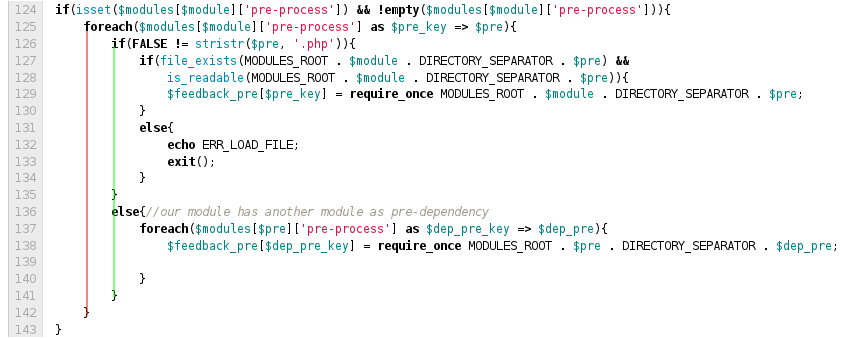
\includegraphics[scale=.5]{cap02/code_align.png}
  \caption{Alinierea codului}
  \label{fig:code_align}
\end{figure}

Observi cum liniile 125 și 142 sunt aliniate vertical. La fel și 126 și 141. Astfel ochiului uman (cu puțin de antrenament)
îi este foarte ușor să își dea seama care acoladă cui aparține.

În continuare, toate listările vor respecta în continuare aceeași convenție de formatare a codului
în mod consistent. Nu vor mai fi introduse explicit unele convenții, însă este bine să fii atent
la aceste detalii pe măsură ce avansezi.

Încă o mică convenție nescrisă: identificatorii \texttt{foo} și \texttt{bar} sunt folosiți ca înlocuitori
pentru ceva fără semnificație. În cazul lor, programatorul vrea să sublinieze că nu variabilele respective
în sinea lor sunt importante, ci alte concepte atașate lor.

\section{Input și formulare}
Atunci când utilizatorul introduce date, pe care le numim colectiv \textsl{input},
acele date trebuie salvate în ceva pentru a avea acces la acele date. Iar cel
mai la îndemână loc de a le salva sunt variabilele.

Una dintre variabilele în care PHP salvează automat un anumit tip de input este \get.
Pentru a o popula cu valori, un utilizator trebuie să introducă ceva în \textsl{request line}-ul
cererii HTTP.

Deci crează un script \texttt{get.php} cu următorul conținut, ca să vezi ce conține variabila \get:
\begin{lstlisting}
<?php
var_dump($_GET);
\end{lstlisting}
Apoi crează o cerere HTTP cu telnet:
\begin{verbatim}
GET /get.php HTTP/1.1
Host: localhost

\end{verbatim}
Întreaga comunicație va arăta cam așa:
\begin{verbatim}
GET /webdev/get.php HTTP/1.1
Host: localhost

HTTP/1.1 200 OK
Date: Sun, 06 Jun 2010 20:27:40 GMT
X-Powered-By: PHP/5.3.2
Content-Length: 13
Content-Type: text/html

array(0) {
}
\end{verbatim}
Observăm că {\get} este un array, și că are zero elemente. Altfel spus,
e un array gol. Ceea ce e logic, din moment ce nu pare să fi făcut niciun
pas special pentru a introduce date. Pentru a introduce date cu metoda GET,
trebuie să creăm parametri pe care să-i adăugăm la adresa resursei cerute.
Sintaxa generală este:
\begin{verbatim}
'/path/to/script.php' ['?' <name> '=' <value> ['&' <name> '=' <value>]+ ]
\end{verbatim}
În cuvinte: numele resursei este urmat de semnul întrebării, apoi o serie de
una sau mai multe perechi nume {\glqq}ia valoarea{\grqq} valoare, separate de caracterul
ampersand ('\&').

Deci fă cererea HTTP:
\begin{verbatim}
GET /get.php?foo=bar&answer=42
\end{verbatim}

Vei vedea că \get\ are valoarea:
\begin{verbatim}
array(2) {
  ["foo"]=>
  string(3) "bar"
  ["answer"]=>
  string(2) "42"
}
\end{verbatim}
După cum observi, nu e nimic special la \get, este un array asociativ
cu care putem lucra așa cum am lucrat cu toate array-urile de până acum.
Cheile din array sunt numele parametrilor, iar valorile \ldots Valorile sunt
mereu stringuri!

Asta nu este neapărat un lucru rău, PHP ne scapă de necesitatea de a converti
(cu type casting) explicit atunci când detectează că poate face o conversie
automată, însă mult mai bine este să convertim noi toate inputurile.

PHP decide cum trebuie să convertească anumite tipuri de date în alte tipuri
de date în funcție de \textit{contextul semantic} în care punem acele date. De exemplu
o valoare 'ABC' în contextul semantic al unei expresii booleene este evaluată
ca TRUE.

\attention{Pentru a valida cu adevărat inputul, va trebui să folosim funcții,
însă funcțiile vor fi prezentate abia în capitolul 3. Deci deocamdată ne
prefacem că un simplu type casting și câteva verificări sunt suficiente.
Facem asta pentru a ne educa din start cu ideea necesității validării inputului.

Tehnici de validare complete vor fi prezentate după introducerea funcțiilor.}

Deci vom putea face un calculator care adună două numere a și b
introduse de utilizator, și afișează rezultatul adunării:
\begin{lstlisting}
<?php
echo (int)$_GET['a'],' + ', (int)$_GET['b'], ' = ', $_GET['a'] + $_GET['b'];
\end{lstlisting}
Vizitează adresa \texttt{http://localhost/add.php?a=3\&b=4}.

Dar oare ce se întâmplă atunci când unul dintre parametri este inexistent?
Hai să vedem. Vizitează direct \texttt{http://localhost/add.php}. PHP îți
va spune ce ai greșit. Mesajul în browser este dificil de citit, deci
folosește opțiunea {\glqq}view source{\grqq} a browserului tău. În firefox, poți apăsa
\keystroke{CTRL+U}.

PHP ne spune ceva de genul
\begin{verbatim}
Undefined index: a in add.php on line 2
\end{verbatim}
pentru fiecare acces la indexul (cheia) 'a' respectiv 'b'
de pe linia 2. Astfel de mesaje ar putea fi utile unui
atacator care ar putea deduce din mesajele afișate cam cum
arată codul tău sursă. Ar putea folosi acele deducții pentru
a-ți sparge site-ul.

Din acest motiv vrem să verificăm mai întâi
dacă cheile 'a' respectiv 'b' există într-adevăr în \get\ \textit{înainte}
de a accesa acei membri ai array-ului. Dacă ambii membri 'a'
și 'b' nu sunt prezenți, atunci afișăm un mesaj de eroare,
altfel facem calculele, pentru că avem cu ce. În acest fel,
orice ar introduce un eventual atacator, acesta nu ar
vedea informații importante pentru el pe care noi nu vrem
să le dezvăluim despre codul nostru sursă:
\begin{lstlisting}[label=lst:addition,caption={Un calculator simplu}]
<?php
if(!isset($_GET['a']) || !isset($_GET['b'])) {
  echo 'Introdu a si b.';
}
else {
  echo (int)$_GET['a'],' + ', (int)$_GET['b'], ' = ', $_GET['a'] + $_GET['b'];
}
\end{lstlisting}
După cum știi, operatorul de negație în PHP este !. El inversează practic valoarea
de adevăr a expresiei logice care urmează. În cazul nostru inversează
valoarea de adevăr a constructului isset(),
care are în interior pe rând parametrii \verb|$_GET['a']| respectiv  \verb|$_GET['b']|.
\begin{Exercise}[title={Înțelege expresia logică},difficulty=1]
\ExePart
Cum se citește linia 2 din listingul \ref{lst:addition}? Începe răspunsul așa:\\
\textit{Dacă \ldots}.

\ExePart

Rescrie condiția într-o formă {\glqq}mai compactă{\grqq} folosind legile lui De Morgan.
Explică încă o dată cum se citește această nouă linie de cod, așa cum
ai făcut în partea I a exercițiului pentru condiția inițială.
\end{Exercise}

\good{Mereu caută să-ți rescrii expresiile logice cu ajutorul
legilor lui De Morgan astfel încât să conțină cât mai multe conjuncții logice.
Asta îți va face scriptul mai rapid, deoarece într-o conjuncție logică, de îndată
ce s-a întâlnit o valoare FALSE, expresiile următoare din acea conjuncție
nu mai sunt evaluate, pentru că nu mai are rost: întreaga conjuncție logică
va avea oricum valoarea de adevăr FALSE.

Deci dacă în exemplul nostru ar fi mai probabil să nu existe 'b', dar să existe 'a',
atunci ar fi mai bine să verificăm mai întâi dacă 'b' este setat. Asta ne-ar economisi
nevoia de a-l verifica și pe 'a'.

În exemplul nostru micuț nu este neapărat cazul, șansele statistice ca un
utilizator răuvoitor să nu seteze ori 'a' ori 'b' sunt practic egale. Însă reține
această modalitate de optimizare pentru situațiile mai complexe.

De exemplu, de preferat ar fi să verifici mai întâi unele variabile introduse de
utilizator, și abia apoi să verifici conjunctiv valori dintr-o bază de date, deoarece
operațiile precum căutările în baze de date sunt mult mai scumpe în termeni
de performață.
}

\begin{Exercise}[title={Un calculator complet},difficulty=2]
Crează un script care acceptă doi parametri obligatorii 'a' și 'b' și un parametru
opțional 'op' care ia ca valori 'add', 'sub', 'mul', 'div' sau 'mod' pentru fiecare
dintre operațiile adunare, scădere, înmulțire, împărțire și modulo.

Dacă parametrul 'op' nu este specificat, atunci trebuie să calculeze rezultatul
tuturor operațiilor $a+b,a-b,a*b,a/b$ și $a\%b$ și să le afișeze rezultatul. Dacă este
specificat, scriptul trebuie să calculeze doar operația corespunzătoare și
să-i afișeze rezultatul.

Folosește constructul \texttt{switch} pentru a decide ce operație trebuie să faci.
Provocarea constă în a nu scrie cod repetitiv.

\textit{Cod repetitiv} înseamnă că ai o secvență de una sau mai multe instrucțiuni identice
în mai multe locuri din algoritm.
\end{Exercise}

\subsection{Formulare, business logic și view logic}

Însă utilizatorul de rând nu ar trebui să aibă cunoștințe tehnice pentru a-ți
trimite date către procesare. Pentru asta există formulare HTML.

Numele câmpurilor de input (atributul \texttt{name}) vor fi folosite \textit{de browser}
pentru a genera URL-ul corect, dacă formularul este
trimis prin metoda GET. De exemplu, un script de întâmpinare a
vizitatorului ar putea arăta astfel:
\begin{lstlisting}
<?php
$mesaj = NULL;
if(isset($_GET['submit'])) {
  if(isset($_GET['nume']) && $_GET['nume']) {
	$mesaj = 'Salut '.$_GET['nume'];
  }
  else {
	$mesaj = 'Eroare: Nu ai introdus numele.';
  }
}
echo $mesaj;
?>
<form method="get">
<label for="nume">Nume:</label>
<input type="text" name="nume" id="nume" />
<input type="submit" name="submit" value="saluta-ma" />
</form>
\end{lstlisting}
Scriptul este constituit din două părți: liniile 2-10 se ocupă de procesarea
formularului. Liniile 11-17 se ocupă de generarea outputului pe baza datelor
procesate.

Transmiterea de informații din procesare către generarea de output se face
folosind \textsl{variabila intermediară} \$mesaj. Deoarece ea va avea ca valoare un
string, o inițializăm cu valoarea NULL, pe linia 2.

Dacă condiția de pe linia 3 este adevărată, înseamnă că utilizatorul a apăsat
butonul {\glqq}submit{\grqq}. În acest caz, vrem să procesăm formularul.

Indiferent
dacă formularul a fost trimis sau nu, 
afișăm direct mesajul, care e NULL dacă formularul nu a fost trimis, deci nu rezultă niciun output în
urma executării liniei 11, și afisăm și formularul.

Dacă formularul nu a fost trimis, atunci cel mai probabil vizitatorul tocmai a intrat
pe pagina noastră și urmează să-l completeze și să-l trimită.

Linia 4 verifică dacă \texttt{\$\_GET['nume']} este setat, și dacă da, verifică
și dacă valoarea salvată în el este evaluată boolean ca fiind TRUE. Altfel spus,
verifică și dacă stringul nu este gol (\texttt{''}) sau nu are valoarea '0'.

Dacă toate acestea sunt adevărate, se generează o valoare dinamică ca mesaj de salut pe linia 5.
Altfel valoarea dinamică va fi un mesaj de eroare, inițializat pe linia 8.

Procesarea formularului de pe liniile 2-10 se numește și \textsl{business logic}.
Acea secvență
din cod validează inputul și setează variabila intermediară \$mesaj în concordanță
cu acest input, sau cu absența inputului.

Variabila intermediară \$mesaj salvează în ea ceea ce numim {\glqq}informație atomară a aplicației{\grqq}.
Se numește așa deoarece, cel puțin în scriptul nostru, constituie o bucățică de informație
indivizibilă, de sine stătătoare.

Generarea outputului pe baza variabilelor intermediare (aici liniile 11-17) constituie
\textsl{view logic} -- logica de vizualizare.

Am fi putut genera output și direct pe liniile 5 respectiv 8, inclusiv formularul,
însă separând \textsl{business logic} de \textsl{view logic},
putem modifica și adapta mai ușor scriptul la noi nevoi.

Logica din spatele aplicației nu are nimic de-a face cu modul ei de prezentare, iar
asta ar trebui să fie reflectat și de codul însuși. Una este validarea inputului,
alta este afișarea.

Mai târziu vei vedea că vei putea genera tot felul de formate de output, nu numai HTML,
cu mai multă ușurință, deoarece business logic va rămâne același, și va trebui
doar să introduci un nou view logic pe baza variabilelor intermediare pe care business logic
ți le pune la dispoziție.

\good{Separă view logic de business logic și introdu variabile intermediare exact
acolo unde este nevoie, variabile care salvează doar informațiile atomare de la baza
aplicației.}

\begin{Exercise}[title={View Logic și Business Logic},difficulty=1]
Îmbunătățește scriptul scris ca soluție la exercițiul {\glqq}Un calculator complet{\grqq},
adăugând un formular care să fie trimis prin metoda POST în loc de GET.

Datele trimise prin POST sunt puse de PHP în array-ul \texttt{\$\_POST}.

Separă business logic de view logic, exact ca în exemplul anterior, folosind
variabile intermediare.
\end{Exercise}

\bad{Deși poți salva valori în array-uri precum \get sau \texttt{\$\_POST}, nu
este bine să o faci. Array-uri ca acestea sunt gândite pentru a prelua
input de la utilizator, sunt populate automat de PHP.

Altfel spus, ele au semantica de input, deci nu ar trebui să le încalci
semantica salvând datele tale proprii în ele.}

%FIXME explicatiile despre VL si BL din 12 ian. 2011 ora 18:25 de pe IRC

\section{Array-uri multidimensionale}
Array-urile sunt structuri de date compozite în care putem salva valori.
Însă un array însuși este o valoare. Din asta deducem inductiv că
putem avea array-uri în array-uri.

Un array bidimensional are două dimensiuni, și ar putea fi inițializat
astfel:
\begin{lstlisting}
$array_2d = array(
  array('foo'),
  array('bar')
);
echo '<pre>';
var_dump($array_2d);
echo '</pre>';
\end{lstlisting}
Bineînțeles că putem refolosi variabile în care am salvat anterior array-uri
pentru a crea noi array-uri. De exemplu, un array tridimensional ar putea arăta
astfel:
\begin{lstlisting}
$array_3d = array(
  'one' => $array_2d,
  'two' => $array_2d
);
var_dump($array_3d);
\end{lstlisting}
Putem crește oricât în dimensiuni, sau putem chiar avea un array cu dimensiuni variabile:
\begin{lstlisting}
<?php
$array_multidim = array(
  $array_2d,
  array('inner 2d' => $array_2d,$array_3d),
  $array_2d
);
var_dump($array_multidim);
\end{lstlisting}

După cum știi deja, array-urile sunt îndeosebi utile atunci când vrem să procesăm anumite date
cu același (sub)algoritm.

Un exemplu pragmatic ar fi să-i cerem utilizatorului să bifeze fructele sale preferate,
și pe baza lor să afișăm anumite informații despre ele.

În formularul HTML nu va trebui decât să numim câmpurile de input cu {\glqq}[]{\grqq}, exact așa cum
am accesa și array-urile în PHP. Pentru o serie de checkbox-uri am putea avea:
\begin{lstlisting}[language=HTML]
<form method="POST">
  <input type="checkbox" name="fructe[]" value="mere" />
  <input type="checkbox" name="fructe[]" value="pere" />
</form>
\end{lstlisting}
Am putea și denumi acele intrări dacă în PHP semantica datelor nu este
de o înșiruire, ci un set de date asociative:
\begin{lstlisting}[language=HTML]
<form method="POST">
  <input name="fructe[mere]" />
  <input name="fructe[pere]" />
</form>
\end{lstlisting}

Un exemplu complet pentru un astfel de script ar putea arăta astfel:
\begin{lstlisting}[label=lst:favourite-fruits,caption={Fructe favorite}]
<?php
$fructe = array(
  'mere' => 'Merele contin multi antioxidanti.',
  'pere' => 'Perele sunt bogate in vitamina C si in potasiu.',
  'alune' => 'Alunele sunt bogate in proteine, grasimi nesaturate si vitamina B6.'
);
if(isset($_GET['submit']) && isset($_GET['fructe'])) {
  foreach($_GET['fructe'] as $fruct) {
	echo '<p>',$fructe[$fruct],'</p>';
  }
}
?>
<form method="GET">
  <input type="checkbox" name="fructe[]" value="mere" id="mere-id" /> <label for="mere-id">Mere</label>
  <input type="checkbox" name="fructe[]" value="pere" id="pere-id" /> <label for="pere-id">Pere</label>
  <input type="checkbox" name="fructe[]" value="alune" id="alune-id" /> <label for="alune-id">Alune</label>
  <input type="submit" name="submit" value="Trimite" />
</form>
\end{lstlisting}

Liniile 14-16 sunt foarte repetitive, și deși putem proceda ca în exemplul de mai sus punând câte un
checkbox, un label, și o intrare în array-ul \$fructe care conține informațiile efective, acest lucru e foarte
ineficient și mănâncă timp dacă vrem să personalizăm acest script.

\good{Când ai linii de cod repetitive foarte asemănătoare din punct de verede structural,
cel mai probabil poți face acele lucruri într-o buclă. Folosește aceste bucle pentru a
reduce costurile de mentenanță (și modificare) a codului, deci implicit și pentru
economisirea timpului. Astfel devii mai productiv.}

Ce se întâmplă dacă vrem să adăugăm sau
să ștergem un fruct? Trebuie să o facem în trei locuri!

Practic însă avem toate informațiile de care avem nevoie (lista de fructe posibile) în array-ul \$fructe,
deci putem folosi acele informații pentru a genera formularul HTML.

\begin{Exercise}[title={Structuri de date abstracte},difficulty=1]
Modifică scriptul din listingul \ref{lst:favourite-fruits} astfel încât să genereze dinamic
formularul HTML pe baza structurii de date asociative \$fructe.

Îmbunătățește scriptul astfel încât să nu dea erori pentru inputuri precum\\
\texttt{/fructe.php?fructe[]=capsuni\&submit=Trimite}
\end{Exercise}

\good{După cum observi, deja ai învățat o grămadă de lucruri care îți pot
ușura munca și economisi timp și îți oferă și flexibilitate.

Tot ce trebuie acum să faci e să reflectezi asupra lucrurilor învățate și să îți
imaginezi cum le-ai putea combina.

Ai la dispoziție variabile și structuri de date, ramificări condiționale ale
fluxului de execuție, și bucle.
}

\subsection{Geometria și normalizarea array-urilor}
Geometria unui array descrie felul în care arată un array. O caracteristică
a geometriei este numărul de dimensiuni a array-ului și/sau a fiecărui câmp.

De exemplu putem stabili că un câmp \texttt{pasiuni} este o listă de pasiuni,
deci pe undeva în aplicație putem avea:
\begin{lstlisting}
$pasiuni = array('tenis', 'fotbal', 'balet');
\end{lstlisting}

Structurile\footnote{Array-urile} de date pot crește însă în complexitate, de
exemplu putem descrie o persoană cu următoarea listă de meta-date:
\begin{lstlisting}
$persoana = array(
  'nume' => 'Xulescu',
  'varsta' => 15,
  'liceu' => 'George Enescu',
  'pasiuni' => array('tenis', 'fotbal', 'balet')
);
\end{lstlisting}
Meta-datele precum \texttt{nume} sau \texttt{pasiuni} sunt fixe, dar valorile
pot varia de la om la om. Cert este că un câmp \texttt{varsta} va fi mereu
integer, iar \texttt{pasiuni} va fi mereu un array.

Dar ce se întâmplă dacă o persoană nu are pasiuni? Simplu: lista de pasiuni
poate fi goală:
\begin{lstlisting}
$persoana = array(
  'nume' => 'Xulescu',
  'varsta' => 15,
  'liceu' => 'George Enescu',
  'pasiuni' => array()
);
\end{lstlisting}
În acest fel, chiar dacă nu avem pasiuni, structura de date în întregimea sa
respectă în continuare geometria prestabilită a array-ului.

Ce se întâmplă dacă în cadrul aplicației noastre stabilim și că
o persoană poate avea și caracteristici precum \texttt{facultate}
sau \texttt{limbi\_cunoscute}? Va trebui să adăugăm și aceste caracteristici,
pentru a păstra array-ul normalizat, chiar dacă persoana respectivă nu are
o anumită \texttt{facultate} drept caracteristică.

Obținem:
\begin{lstlisting}
$persoana = array(
  'nume' => 'Xulescu',
  'varsta' => 15,
  'liceu' => 'George Enescu',
  'facultate' => NULL,
  'limbi_cunoscute' => array('romana'),
  'pasiuni' => array()
);
\end{lstlisting}

Atunci când aducem o structură de date la cea mai complexă formă a sa,
spunem că am \textsl{normalizat} acea structură, sau că am adus-o la o \textsl{formă
canonică}.

\section{Sisteme de numerație}
\subsection{Baze numerice}
Pentru a înțelege operațiile binare, trebuie să înțelegem mai întâi sistemele
de numerație.

Primul sistem de numerație pe care l-ai învățat și cu care te simți cel
mai confortabil este sistemul decimal. Se numește astfel deoarece
ai la dispoziție zece simboluri, fiecare din ele reprezentând o cantitate:
0, 1, 2, 3, 4, 5, 6, 7, 8, 9.

Trebuie să facem însă distincția clară între cantitate și reprezentarea
acesteia. În cazul nostru, cantitatea doisprezece are reprezentarea 12.

Dar ce se întâmplă când numărăm? Cum numărăm de fapt? Ai învățat
asta când erai copil și ți-a intrat atât de adânc în procesele cognitive,
încât nici nu mai poți conștientiza ce faci când numeri de fapt.

Când numeri, iei pe rând simbolurile pe care le ai la dispoziție 0, 1, 2, 3, 4, 5, 6, 7, 8.
O dată ajuns la 9, nu mai ai simboluri, deci adaugi unu la poziția imediat din
stânga, și încă unul la poziția la care ești, în cazul nostru la poziția unităților.

Asta e posibil deoarece reprezentarea
\begin{verbatim}
9
\end{verbatim}
este același lucru cu
\begin{verbatim}
09
\end{verbatim}
sau cu oricâți de 0 în față, nu contează:
\begin{verbatim}
00000009
\end{verbatim}
Deoarece după ultimul simbol, în cazul nostru 9, urmează primul simbol, deci 0, și invers,
deoarece înaintea lui 0 se află simbolul 9, spunem că acest șir de simboluri
0, 1, 2, 3, 4, 5, 6, 7, 8, 9, este un \textsl{șir circular}. Ca o analogie
la ce înseamnă \textit{circular}, gândește-te la un lacăt cu cifru.
Așa se face că după 009 urmează 010, adică zece.

Până acum am numărat în baza 10. Acum hai să generalizăm. Să zicem că avem
simbolurile s,t,u,v, și vrem să numărăm crescător în baza 4, deoarece avem
patru simboluri. Pentru asta nu trebuie decât să luăm simbolurile la rând:
\texttt{s}, \texttt{t}, \texttt{u}, \texttt{v}.
O dată ajunși la \texttt{v}, nu mai avem simboluri, deci trebuie să sărim
pe poziția următoare și să adăugăm cantitatea 1.

Cum pe poziția următoare
se află s (similar cu acel 0 {\glqq}invizibil{\grqq} din baza 10), și deoarece după v
urmează s, deducem că după \texttt{v} urmează \texttt{ts}, care reprezintă
deci cantitatea 4. În continuare ar urma
\texttt{tt}, \texttt{tu}, \texttt{tv}, 
\texttt{us}, \texttt{ut}, \texttt{uu}, \texttt{uv}, \ldots, vv, \ldots,
\texttt{tss}, \texttt{tst}, \texttt{tsu}, \texttt{tsv},
\texttt{tts}, \texttt{ttt}, \ldots, \texttt{vvs}, \texttt{vvt},
\texttt{vvz}, \texttt{vvv}, \texttt{tsss}, \ldots

\begin{Exercise}[title={Numără în baza șapte},difficulty=2]
Numără până la cantitatea două zeci în baza șapte folosind setul
de simboluri ordonate d, g, h, a, s, z, u.
\end{Exercise}

Orice bază de numerație, fie ea binară (2), octală (8) sau
hexadecimală (16) funcționează după exact aceleași principii.

Demn de menționat este că în PHP, valorile pot fi introduse
folosind reprezentarea lor octală punând zero în fața lor, iar
valorile hexadecimale pot fi introduse direct prefixându-le cu 0x.
Pentru reprezentarea hexadecimală se folosesc pe rând literele A, B, C,
D, E, F care urmează după simbolul 9.
Exemple:
\begin{lstlisting}
<?php
$foo = 052;
echo $foo,' ', 0x2A;
\end{lstlisting}

\subsection{Operații pe biți}
Există șase operații binare în PHP, iar înțelegerea lor este
foarte ușoară dacă ai înțeles deja expresiile booleene și
operațiile logice prezentate în paginile
\pageref{sec:tipul de date boolean. Expresii logice}--\pageref{endsec:tipul de date boolean. Expresii logice}.

Plecând de la reprezentarea binară a două cantități, de exemplu \texttt{00101010} și
\texttt{01100111}, putem uni conjunctiv fiecare bit cu bitul corespunzător din a doua valoare.
1 este același lucru cu TRUE iar 0 același lucru cu FALSE din tabelul \ref{tbl:truth table and or}.
Această operație se numește \textsl{binary and}, iar operatorul PHP este \texttt{\&}.
Calculăm:
\begin{verbatim}
00101010 &
01100111
--------
00100010
\end{verbatim}

Operația disjunctivă se numește \textsl{binary or}, și are operatorul |. Calculăm:
\begin{verbatim}
00101010 |
01100111
--------
01101111
\end{verbatim}

Mai putem muta și la dreapta șirul de biți cu un număr de poziții. Operatorul
pentru asta este \texttt{$>>$} și se numește \textsl{shift to right}. Exemplu:
\begin{verbatim}
00101010 >> 3 = 00000101
\end{verbatim}

Un octet (en. \textsl{byte}) este un șir de opt biți,
iar un bit este 0 sau 1. În exemplele de mai sus am făcut deci operațiile binare
\textit{and} și \textit{or} pe reprezentarea într-un byte a doi operanzi.

În PHP, numerele întregi ocupă un anumit număr de bytes. Acesta este dependent de
platformă, și este de obicei 4 sau 8. Află cât spațiu au la dispoziție numerele
întregi:
\begin{lstlisting}
<?php
echo PHP_INT_SIZE,PHP_EOL;
\end{lstlisting}

Acum știm tot ce trebuie pentru a afișa reprezentarea binară a oricărui număr:
\begin{lstlisting}[label=lst:bitbybit,caption={Afișarea bit cu bit a unui int}]
<?php
$a = 42;
for($i=8*PHP_INT_SIZE-1;$i>=0;$i--) {
  echo ($a>>$i) & 1 ? '1':'0';
}
\end{lstlisting}

\attention{În urma operației \textit{shift to right} cu X biți, se pierd cei mai din
dreapta X biți, iar în partea din stânga X biți (care apar {\glqq}noi{\grqq}) sunt inițializați
cu zero.}

\begin{Exercise}[difficulty=3,title={Cum funcționează afișarea bit cu bit a unui int?}]
Explică cum funcționează codul din listingul \ref{lst:bitbybit}.

Concentrează-te
în special pe expresia \texttt{(\$a$>>$\$i) \& 1}.

Experimentează și fă observații pe baza experimentelor. Ai putea citi și articolul
de pe wikipedia.\footnote{\url{http://en.wikipedia.org/wiki/Bitwise_operation}}
\end{Exercise}

Analog cu \textit{shift to right}, există și un \textsl{shift to left}. Operatorul este
\texttt{$<<$}, după cum poți vedea \^in listingul \ref{lst:shiftleft}.
\begin{lstlisting}[label=lst:shiftleft,caption={Operatorul shift to left}]
<?php
$a = 42;
for($i=8*PHP_INT_SIZE-1;$i>=0;$i--) {
  echo ($a>>$i) & 1 ? '1':'0';
}
$a <<= 5;
echo PHP_EOL;
for($i=8*PHP_INT_SIZE-1;$i>=0;$i--) {
  echo ($a>>$i) & 1 ? '1':'0';
}
\end{lstlisting}
După cum observi pe linia 6, putem contracta operațiile binare cu operația de atribuire
într-o singură operație.

Similar cu shift to right, biții din dreapta sunt inițializați automat cu 0, iar cei din
stânga se pierd. 

O altă operație este \textsl{inversarea} sau \textsl{negarea} biților. 0 devine 1, iar 1 devine 0.
În contrast cu operațiile de până acum, inversarea biților\footnote{La fel ca negarea
booleană, unde !<expr> are valoarea de adevăr inversă a expresiei.} are un singur operand.
Operatorul este $\sim$ și se pune în fața operandului: 
\begin{lstlisting}
<?php
$a = 42;
for($i=8*PHP_INT_SIZE-1;$i>=0;$i--) {
  echo ($a>>$i) & 1 ? '1':'0';
}

echo PHP_EOL;
$a = ~42;
for($i=8*PHP_INT_SIZE-1;$i>=0;$i--) {
  echo ($a>>$i) & 1 ? '1':'0';
}
\end{lstlisting}

Ultima operație binară este \textsl{exclusive or}, sau pe scurt
\textsl{xor}. Operatorul este \textasciicircum, și
acceptă doi operanzi. În algebră booleană, am descrie această operație așa:
\[(\lnot a \land b) \lor (a \land \lnot b)\]

\begin{Exercise}[title={Jonglează cu expresii boolene},difficulty=3]
Explică în limba română, pe baza definiției operației xor
$(\lnot a \land b) \lor (a \land \lnot b)$,
în ce situații este foarte utilă această operație.
\end{Exercise}


%TODO modifica acest exercitiu, adauga mai multe explicatii,
% probabil va trebui sa transform exercitiul in explicatii din text,
% iar exercitiul sa devina "rescrie a.i. sa fie shift-uit 1, nu inputul" (catch: nu se va spune
% ca trebuie shiftuit la stanga)
\begin{Exercise}[title={Operații pe biți}]
Crează un script care acceptă două numere a și b, cu b mai mic sau egal cu 8*PHP\_INT\_SIZE-1, și
care afișează rezultatele operațiilor \texttt{a\&b}, \texttt{a|b}, \texttt{a$<<$b},
\texttt{a$>>$b}, \texttt{a{\textasciicircum}b},
\texttt{{\texttildelow}a}, \texttt{{\texttildelow}b} și \texttt{(a$>>$b)\&0x1}.
\end{Exercise}

Operațiile pe biți sunt foarte utile atunci când vrem să setăm atribute booleene {\glqq}da sau nu{\grqq}
pentru anumite proprietăți, drepturi de acces, etc. Avantajul este că aceste câmpuri de biți
(en. \textsl{bitfields}) sunt foarte compacte, ocupă puțin spațiu.

Un scenariu de utilizare:
\begin{lstlisting}
<?php
const AUTH_NONE = 0x00;
const AUTH_READ = 0x01;
const AUTH_WRITE = 0x02;
const AUTH_DELETE = 0x04;

$drepturile_mele = AUTH_READ|AUTH_WRITE|AUTH_DELETE;

if($drepturile_mele & (AUTH_READ|AUTH_WRITE)) {
  echo 'poti citi si scrie<br>';
}
\end{lstlisting}
Liniile 2-5 inițializează constante cu drepturile respective.  Cantitățile 1, 2 și 4
au fiecare biții doar câte un bit setat, de la dreapta la stânga, 1 are primul bit setat,
2 are al doilea bit setat, 4 îl are doar pe al treilea setat. Astfel nu avem conflicte
între cele patru niveluri de acces. Folosim constante
deoarece acei biți nu se schimbă niciodată.

Linia 7 unește conjunctiv toate drepturile de acces, ceea ce rezultă practic în șirul
de biți \texttt{00000111}.

Linia 9 verifică conjunctiv dacă drepturile utilizatorului care vizitează
momentan pagina include și bitul AUTH\_READ. După evaluarea condiției
de pe linia 9 ne alegem fie cu valoarea 0, fie cu o altă valoare,
care conform observațiilor pe care le-ai făcut în listingul \ref{lst:typecasting}
va fi evaluată ca TRUE.

Teoretic am fi putut folosi și un array asociativ, de exemplu:
\begin{lstlisting}
<?php
$drepturile_mele = array(
  'read' => TRUE,
  'write' => TRUE,
  'delete' => TRUE
);
if($drepturile_mele['read'] && $drepturile_mele['write']) {
  echo 'poti citi si scrie<br>';
}
\end{lstlisting}
însă ocupă mult mai mult spațiu și nu este la fel de compact.
În plus, bitfield-urile pot fi salvate mult mai ușor în alte
sisteme precum baze de date, poți sorta după anumite valori, ș.a.m.d.

\section{Variabile variabile}
O variabilă variabilă se numește astfel deoarece îi construim numele (identificatorul) variabil,
pe baza altor valori. Pentru a crea o variabilă variabilă, folosim \$, urmat de identificatorul unei variabile,
care după cum știm, începe tot cu \$. Deci ne alegem cum două simboluri \$\$ unul după altul.

Exemplu:
\begin{lstlisting}
<?php
$a = 'b';
$$a = 'c';
var_dump($b);
\end{lstlisting}
După cum observi, nu declarăm nicăieri o variabilă \$b, însă o folosim pe linia 4.
Variabila \$b este creată pe linia 3, pe baza valorii variabilei \$a.

Putem chiar crea variabile din array-uri asociative, de exemplu:
\begin{lstlisting}[label=lst:varvarfromassoc,caption=Variabile variabile din array asociativ]
<?php
$variabile = array(
  'foo' => 'bar',
  'foobar' => 'barfoo'
);
foreach($variabile as $nume => $valoare) {
  $$nume = $valoare;
}
echo "$foo $foobar";
\end{lstlisting}

Atunci când creăm o variabilă (variabilă sau nu, nu contează), PHP îi pune identificatorul și valoarea
într-un tabel. Acest tabel se numește \textsl{scopul global} de variabile (en. \textsl{variable global scope}).

Folosind variabile variabile, poluăm acest \textit{scope}, iar asta este o practică rea.
Există unele situații în care variabilele variabile sunt utile, dar acestea implică
alte \textit{scope}-uri, nu cel global. Un astfel de exemplu\footnote{Și singurul în care
folosirea variabilelor variabile este legitimă, după părerea autorului.} îl vom întâlni
în capitolul următor.

\section{Referințe}
După cum știi, variabilele create sunt salvate de PHP într-un tabel cu identificatorul
și valoarea variabilei.

Referințele sunt ca niște nume alternative pentru aceeași valoare. Pentru a crea o referință,
punem '\&' în fața identificatorului variabilei pe care vrem să o referențiem. Exemplu:

\begin{lstlisting}
<?php
$a = 42;
$b = &$a;
echo $a,' ';
$b++;
echo $a;
\end{lstlisting}
Conform liniei 3, identificatorul \$b va {\glqq}arăta cu degetul{\grqq} (en. \textsl{point at})
către conținutul variabilei \$a. Pe linia 5 incrementăm acea valoare, însă prin prisma
identificatorului \$b.

Din moment ce și \$a, și \$b, arată către aceeași intrare din tabelul
\textit{\textit{scope}-ului global}, lucrul care
se reflectă și asupra valorii variabilei \$a pe linia 6.

\section{Exerciții}

\begin{Exercise}[title={Terminologie},difficulty=1]
În acest capitol ai învățat o grămadă de termeni noi.
Folosind cuprinsul de la pagina \pageref{cuprins},
ia fiecare secțiune a acestui capitol la rând, și la fiecare
scrie \textit{cel puțin} un cuvânt sau expresie,
fie el în română sau în engleză. La termenii în română,
scrie și corespondenții englezești.

Gândește-te cât știai înainte de a citi acest
capitol. Cum te simți? Eu m-aș simți mândru.
Felicitări!
\end{Exercise}

\begin{Exercise}[title={Rezumat},difficulty=2]
Explică în cel puțin 500 de cuvinte cum funcționează lucrurile pe care le-ai învățat și înțeles în acest
capitol. Folosește propriile formulări (fără copy/paste), și folosește cât mai mulți termeni
pe care i-ai găsit în exercițiul anterior.

Încearcă să sintetizezi cât mai multe lucruri care nu au fost spuse explicit, dar pe care
le poți deduce. Fă brainstorming\footnote{\url{http://en.wikipedia.org/wiki/Brainstorming}}
cu tine însuți, analizează conceptele
pe care le explici în rezumat.

Încearcă să te gândești cât mai serios și să reflectezi
asupra celor învățate.
De exemplu, gândește-te și explică ce legătură are conceptul de \textit{context semantic} cu
restul noțiunilor învățate în acest capitol (spre exemplu noțiunea de \textit{expresie} în PHP,
fie ea booleană, matematică, sau cu stringuri).

Nu te teme să faci afirmații îndrăznețe pentru a arăta că știi să gândești \textit{out
of the box}, deci că ai potențialul de a fi inovativ. Chiar dacă afirmațiile vor
fi greșite, este foarte probabil să înveți lucruri noi, pentru că-i faci 
pe tutorii {\phpro} să te corecteze și automat să vină cu explicații din care
să înveți lucruri noi, sau care îți clarifică unele lucruri. Sau cine știe,
poate ai o întrebare a cărei răspuns e atât de complex încât îi blochezi
pe tutori :-)
\end{Exercise}

\begin{Exercise}[title={Language Reference}]
Acest capitol a încercat să îți ofere o imagine cât mai clară a conceptelor
de bază, însă e foarte probabil ca unele noțiuni ori să nu fi fost
abordate cu destul de multă atenție la detalii, ori să nu fi fost abordate deloc.

PHP este documentat foarte bine în ceea ce numim \textit{manualul PHP}. Adresa
sa oficială este \url{http://php.net/manual}.

Intră pe manualul PHP și urmează cu atenție toate paginile din capitolul
\textit{Language Reference}.\footnote{\url{http://php.net/langref}}

\good{Citește exclusiv versiunea engleză a manualului. Este cea mai actuală
și cea mai corectă versiune. NU citi traducerea sa în română. Astfel
te vei și obișnui să lucrezi cu engleza, ca un viitor profesionist.}

Găsește cel puțin 5 lucruri care nu au fost spuse în carte și pe
care le-ai putut înțelege în urma citirii acelui capitol din manual.
% backtick - execution operator
% @$array[$index] suprima erori dacă $index nu există
% <> este același lucru ca !=
% << si >> inseamna inmultirea cu 2
% variabile predefinite _SERVER, etc
\end{Exercise}

\begin{Exercise}[title={Scrie scripturi}]

\ExePart

Scrie trei scripturi, fiecare de cel puțin 50 de
LOCs,\footnote{Liniile goale sau care consistă doar din comentarii nu se calculează}
care să aibă în total peste 250 de LOCs, și să rezolve probleme practice sau care
te-au preocupat mereu sau probleme pe care ți le-ai pus pe parcursul studiului acestor
capitole.

Scripturile trebuie să genereze cod XHTML 1.1 curat, și să fie
validate cu succes de \href{http://validator.w3.org/}{validatorul W3C}.\footnote{http://validator.w3.org/}

Fi atent și la accesibilitatea formularelor și generează cod XHTML semantic. Nu uita
să separi \textit{business logic} de
\textit{view logic} și să folosești variabile intermediare.

Posibile probleme de rezolvat:
\begin{itemize}
  \item generează un tabel HTML pe baza unui array bidimensional asociativ și afișează
rândurile din tabel colorate alternativ cu două culori de fundal, pentru o mai bună accesibilitate
  \item citește o sumă de bani (RON) și afișează numărul minim de bancnote din
fiecare sumă: 1, 5, 10, 50, 100, 200, 500, cu care poți acoperi suma introdusă
\end{itemize}

Cere ajutorul comunității de pe {\phpro} acolo unde te blochezi.

\ExePart

Explică pas cu pas unui neprogramator ce face fiecare cod și cum o face.
Nu ai voie să folosești termeni tehnici, ci doar formulări pragmatice.

\end{Exercise}



%php functii, modularizare, separare, securitate, practic: guestbook
\chapter{Reutilizarea și modularizarea codului}

\begin{chapsummary}
Acest capitol îți va prezenta tehnici de reutilizare a codului,
ceea ce-ți va permite să programezi mai eficient. Îți va
mai deschide porțile și către mai toate funcționalitățile
și capacitățile limbajului PHP.
\end{chapsummary}

\section{Funcții}
\subsection{Funcții proprii. Termeni generali}
%retval, args, optional args, references, static variables
O funcție este ca o cutie neagră. O hrănești cu date prin
intermediul a ceea ce numim \textsl{parametri}, și ea
face anumite operații pe acel input primit prin parametri.

Unele funcții generează output, alte funcții returnează
valori și nu afișează nimic, iar altele nici nu acceptă
parametri.

Până acum am întâlnit o singură funcție, \texttt{var\_dump()}.
Ea acceptă un singur parametru,\footnote{Greșeală deliberată.
Voi reveni la lecția despre funcții variadice.} care trebuie să fie o expresie,
și generează ca output valoarea acelei expresii, alături de tipul
de date al expresiei.

Deoarece tipul de date al parametrului acceptat de această funcție
nu trebuie să fie de un anumit fel specific, ci poate avea 
de la două tipuri de date în sus,
spunem că parametrul funcției este de tipul \textsl{mixed}.
Acesta nu este un tip de date existent în PHP, este doar
felul în care putem documenta astfel de valori care pot
avea tipuri de date multiple.

Documentarea funcției var\_dump() ar putea arăta deci astfel:

\begin{verbatim}
void var_dump(mixed $expression)
  - dumps information about an expression
\end{verbatim}

\texttt{var\_dump} se numește \textsl{identificatorul} sau numele funcției.
Acel \texttt{void} din fața lui ne spune ce fel de date returnează funcția. \textsl{void}
este un alt tip de date care de fapt nu există și este folosit doar în documentarea
funcțiilor. \textit{void} înseamnă nimic, deci în cazul nostru, înseamnă că
funcția nu returnează nimic.

Dar cum creăm propriile funcții? Hai să creăm o funcție care nu acceptă nici un
parametru, care nu returnează nimic, dar care doar face ceva. Hai să îi dăm acestei
funcții identificatorul \texttt{foo}. Documentarea ei va arăta deci astfel:
\begin{verbatim}
void foo(void)
\end{verbatim}
Această "documentare" se numește și \textsl{semnătura funcției}, deoarece
ne spune cum arată din exterior acea funcție, ce fel de parametri acceptă
și în ce ordine, și ce fel de date returnează.

Limbajul PHP nu este at\^at de strict \^in privința tipurilor de date
acceptate ca parametri sau tipurilor de date returnate de funcții. De aceea
documentarea semnăturilor funcțiilor noastre ne poate feri pe noi \^inșine
de greșeli de programare. De exemplu, dacă documentăm o funcție ca return\^and
``int'', și la un moment dat, \^in timp ce implementăm acea funcție,
returnăm un ``string'', atunci e clar că am făcut o greșeală, și cel
mai probabil greșeala este \^in implementație.

\good{Atunci c\^and decizi să creezi o funcție, mai \^int\^ai analizează logistica
care impune necesitatea acelei funcții, documentează de ce există acea funcție, ce face,
și semnătura sa. După aceea implementează funcția astfel \^inc\^at să respecte
documentația sa.}




Pe lângă o semnătură, o funcție mai are și o implementație. Toate funcțiile
trebuie implementate înainte de a fi folosite. Pentru a declara
implementația unei funcții în PHP,\footnote{Sau pe scurt: \textit{pentru
a implementa o funcție}}
scriem cuvântul cheie \texttt{function} urmat de identificatorul funcției,
paranteze rotunde, și între ele o listă a eventualilor parametri,
apoi implementația efectivă a funcției între acolade, ca un bloc
de instrucțiuni. Funcția
noastră \texttt{foo} ar putea avea următoarea implementație:
\begin{lstlisting}
<?php
function foo() {
  echo 'bar';
}
\end{lstlisting}
Dacă semnătura funcției se pune \^in documentația funcției, atunci analog cu ea
avem \^in codul PHP efectiv ceea ce numim \textsl{antetul funcției} (en. \textsl{function header}),
\^in exemplul anterior acesta fiind
\begin{verbatim}
foo()
\end{verbatim}


Acum că am implementat funcția, o putem apela. Un exemplu complet:
\begin{lstlisting}
<?php
function foo() {
  echo 'bar';
}
foo();
$i=10;
while($i--) {
  foo();
}
\end{lstlisting}
Pe liniile 5 și 8 spunem că am apelat funcția \texttt{foo}, care poartă numele
de \textsl{callee} sau apelat.

După cum observi, poți folosi constructele învățate în capitolul anterior în
jurul funcțiilor. La fel de bine poți folosi constructele respective
și în implementația funcțiilor. De exemplu, această funcție afișează numerele
de la 0 la 10:
\begin{lstlisting}
<?php
function count_to_10() {
  for($i=0;$i<=10;$i++) {
	echo $i,' ';
  }
}
count_to_10();
\end{lstlisting}

Funcțiile pot accepta și parametri. Putem spune că am parametrizat
funcția sau că am parametrizat algoritmul implementat de acea funcție. Parametrii
adaugă un plus de flexibilitate.


Ce se întâmplă dacă vrem să numărăm
de la 0 la un număr variabil? Algoritmul nu se schimbă, numai că
trebuie să începem de la 0 dar să ne oprim la acel număr specificat
în parametru. Exemplu:
\begin{lstlisting}
<?php
function count_to_n($n) {
  for($i=0; $i<=$n; $i++) {
	echo $i,' ';
  }
  echo '<br />';
}
count_to_n(42);
\end{lstlisting}
Iar documentația funcției ar arăta așa:
\begin{verbatim}
void count_to_n(int $n)
\end{verbatim}

Acel \texttt{int \$n} ne spune că funcția acceptă un parametru care va fi accesibil
din interiorul funcției sub identificatorul \$n, și că tipul de date al acestuia
este integer. În interiorul funcției putem face orice dorim cu acel parametru.

Sau am putea lăsa la o parte identificatorul parametrului în documentație:
\begin{verbatim}
void count_to_n(int)
\end{verbatim}
Asta este posibil deoarece la documentarea funcției nu contează numele parametrului.
Numele parametrului este util doar în implementația funcției, însă noi acum
doar documentăm semnătura funcției, iar în documentație nu trebuie să știm
decât ce tip de date are al X-ulea parametru (aici primul).

În practică însă, este mai bine să spunem și numele parametrului în documentație,
deoarece putem folosi acel identificator al parametrului în descrierea funcționalității
funcției.

\good{Documentează-ți mereu semnăturile funcțiilor tale, cu tot
cu tipurile de date ale parametrilor. Asta te va ajuta să-ți
amintești mai repede cum funcționează propriul tău cod chiar
și după ani de zile în care nu ai lucrat cu acele funcții proprii.}

Pentru a documenta o funcție, scrie-i semnătura deasupra implementăriii,
folosind comentarii. Tot în acele comentarii poți documenta și
ce face fiecare parametru. Exemplu de cod documentat bine:

\begin{lstlisting}
<?php
/**
 * display a space-separated list of numbers, up to $n
 *
 * void count_to_n(int $n)
 */
function count_to_n($n) {
  for($i=0; $i<=$n; $i++) {
	echo $i,' ';
  }
  echo '<br />';
}
\end{lstlisting}

Încearcă să apelezi funcția așa, și observă
ce se întâmplă:
\begin{lstlisting}
count_to_n('foo');
\end{lstlisting}

Cu ajutorul documentației, ți-ai putea da seama ușor care e greșeala,
chiar dacă acel cod este scris de altcineva și îl vezi pentru prima dată.
%TODO CHAP spune ce capitol (phpDocumentor)
Într-un capitol următor vei vedea că există și scule care generează semi-automat
documentație în format HTML, care îți fac navigarea prin cod mai ușoară, 
și care-ți permit să înțelegi cu ușurință cum funcționează aplicații
complexe, chiar dacă acestea îți sunt străine.

\begin{Exercise}[title={Funcție care afișează reprezentarea binară}]
În capitolul trecut a trebuit să scrii de fiecare
dată o buclă atunci când ai vrut să afișezi reprezentarea
binară a unui număr întreg. Cu funcții, nu trebuie
să implementezi acel algoritm decât o singură dată,
să îl ``îmbraci'' într-o funcție, și să apelezi acea
funcție de fiecare dată când ai nevoie de ea. Asta te scapă de
multă muncă inutilă și cod care nu numai că este repetitiv,
dar care mai este și greu de citit.

Scrie o funcție care afișează reprezentarea binară a unui integer.
\end{Exercise}

Afișările făcute în funcții sunt puternice și ne scapă deja de mult
efort. Însă înainte de a ne grăbi să punem o grămadă de \texttt{echo}
în funcțiile noastre, hai să ne întrebăm înainte:\\
\textit{Ce se întâmplă dacă nu vrem să afișăm rezultatul unei funcții, ci să-l
refolosim într-un alt mod?}

Ce se întâmplă dacă nu vrem de exemplu să afișăm reprezentarea binară
a unui număr, ci să o salvăm într-un fișier, o bază de date, sau să
o trimitem prin e-mail?

\textit{Retval comes to the rescue}. \textsl{Retval}, sau corect \textsl{return value},
este valoarea returnată de o funcție. Toate funcțiile pot returna o valoare.

În mod implicit, funcțiile care returnează void, deci care în fapt nu returnează
nimic, returnează de fapt valoarea NULL. Exemplu:
\begin{lstlisting}
<?php
function do_nothing() {
//the do-nothing function is a function
//which has a simple functionality: it does nothing
}
$val = do_nothing();
var_dump($val);
var_dump(do_nothing());
\end{lstlisting}

Pe linia 6, atribuim valoarea returnată de apelul la \texttt{do\_nothing()}
variabilei \texttt{\$val}, și pe linia următoare afișăm această valoare.

Pe linia 8 îi pasăm ca parametru lui \texttt{var\_dump()} direct retval-ul apelului
la \texttt{do\_nothing()}.

\attention{Valoarea returnată de o funcție este tot o valoare (după cum îi spune
însăși numele de return \textit{value}), deci poate fi folosită ca atare
peste tot unde parserul PHP acceptă o valoare.}

Deoarece o valoare este și o expresie, putem pune un apel la o funcție peste tot
unde PHP acceptă o expresie: în condițiile buclelor, între [] pentru a accesa un
anumit index al unui array, ș.a.m.d. Exemplu:

\begin{lstlisting}
if(do_nothing()) {
  echo 'do nothing returns something';
}
\end{lstlisting}
Fluxul de execuție va ajunge la \texttt{if}. O dată ajuns aici, PHP știe că
trebuie să citească o expresie și să o evalueze boolean, deci întâlnește apelul
la o funcție. Deoarece e un apel, funcția se numește și \textsl{apelat},
iar fluxul de execuție trebuie să intre în
acea funcție, să treacă prin implementația funcției,\footnote{Altfel spus, să
apeleze funcția.} și într-un final
să se ajungă la un retval, care în cazul nostru este implicit \texttt{NULL}.

Apoi acest retval este pasat înapoi
apelantului (en. \textsl{caller}),\footnote{Apelantul este entitatea care apelează funcția. În cazul nostru,
este scriptul .php însuși, dar ar putea fi și o altă funcție, deoarece
o funcție poate apela o altă funcție.}
în cazul nostru contextului
semantic de valoare booleană creat de constructul \texttt{if}. O dată ajuns
în acest context, \texttt{NULL}-ul returnat de funcție este evaluat ca \texttt{FALSE}.

Fiind într-o funcție, pentru a returna o anumită valoare în loc
de NULL-ul implicit, trebuie să folosim
constructul \texttt{return}. Sintaxa este simplă și intuitivă:
\begin{verbatim}
return <expr>;
\end{verbatim}

În capitolul trecut am auzit despre \textit{scope}-ul global al variabilelor.
Cu ajutorul funcțiilor, putem vedea în practică ce înseamnă acest \textit{scope}
și ce altfel de \textit{scope}-uri mai există.

Vom discuta pe marginea următorului listing:
\begin{lstlisting}
<?php
function increment($a) {
  $a = 'bar';
  echo "in interior \$a este $a\n";
}
$a = 42;
echo "$a\n";
increment($a);
echo "$a\n";
\end{lstlisting}

Totul ne este cunoscut până la linia 8. La apelarea funcției \texttt{increment()},
parametrul \$a al funcției primește inițial valoarea 42, așa cum ne așteptăm.
Însă fluxul de execuție ajunge pe linia 3, moment în care \$a primește valoarea
constantă 'bar', așa cum ne demonstrează și outputul generat pe linia 4.
Totuși fluxul de execuție revine pe linia 9, moment în care \$a are iar valoarea 42. De ce?

Răspunsul e simplu: parametrul (variabila) \$a al funcției și variabila \$a din scope-ul
global nu au nimic în comun. Sunt două variabile complet diferite.

Variabila \$a din scope-ul global există doar în scope-ul global, iar variabila \$a
folosită ca parametru în interiorul funcției există doar în interiorul funcției.

Voi ilustra asta cu un cod mai sugestiv, redenumind variabila \$a din \textsl{scope}-ul
global:
\begin{lstlisting}
<?php
function increment($a) {
  $a = 'bar';
  echo "in interior \$a este $a\n";
}
$foo = 42;
echo "$foo\n";
increment($foo);
echo "$foo\n";
\end{lstlisting}

Variabila \texttt{\$foo} se află în contextul global, în tabelul cu variabile globale. Atunci când apelăm
funcția \texttt{increment} pe linia 8, ceea ce pasăm funcției nu este variabila \texttt{\$foo}, ci doar
valoarea ei. Această metodă de a pasa parametri se numește \textsl{pass by value}.
Acesta este motivul pentru care cele două scripturi funcționează absolut identic, deși
variabilele sunt numite diferit. Aici nu este vorba despre numele variabilelor, ci de
valorile lor (fluxul de date) și pe unde trece execuția (fluxul de execuție).

În momentul în care fluxul de execuție intră în funcție,
PHP crează un nou tabel de variabile, care,
pentru că e nou, e gol. Ți-ai dat seama de asta, nu?
Orice variabilă declarată sau folosită în această funcție se pierde o dată cu ieșirea
fluxului de execuție din funcție.

PHP vede însă că funcția acceptă și un parametru numit \texttt{\$a}, și îl crează și pe acesta, însă
tot în tabelul de variabile al \textit{scope}-ului \textsl{local} funcției \texttt{increment()}.
Din acest motiv, logica și operațiile din interiorul funcției sunt complet decuplate
de "lumea exterioară".

Datorită faptului că PHP crează și distruge automat scope-uri, dacă în interiorul
unei funcții am face lucruri precum în listingul \ref{lst:varvarfromassoc},
atunci nu am polua scope-ul global. Acele variabile variabile create ar exista
doar în interiorul funcției, și ar fi distruse o dată ce fluxul de execuție
părăsește funcția.


O funcție poate accepta oricâți parametri. În astfel de cazuri, ei trebuie separați
prin virgulă unul de altul. Exemplu:
\begin{lstlisting}
<?php
function add($a, $b) {
  return $a + $b;
}
$foo = add(42,43);
echo $foo;
\end{lstlisting}

\attention{Nu uita că introducerea de noi variabile ar trebui făcută doar
atunci când avem de gând să refolosim acele variabile.}

\good{Atunci când creezi o funcție care returnează valori numerice
ca "statusuri de eroare", crează constante simbolice în afara funcției
pentru aceste statusuri și returnează acele constante simbolice în
loc de numerele efective. Astfel poți schimba valorile efective returnate,
însă cei care îți apelează funcția o vor folosi așa cum au folosit-o mereu,
deoarece numele constantelor simbolice nu se schimbă.}

În exemplul de mai sus, așa cum e el, introducerea variabilei \texttt{\$foo}
este o practică proastă, era suficient să îi pasăm retval-ul
funcției direct lui \texttt{echo}:
\begin{lstlisting}
echo add(42,43);
\end{lstlisting}

Țin să subliniez încă o dată: retval-ul unei funcții este o valoare
ca oricare alta. Este creată transparent pentru noi de PHP, la fel
cum într-un exemplu precum:
\begin{lstlisting}
<?php
'a' . 'b';
\end{lstlisting}
din 'a' și 'b' rezultă o valoare nouă 'ab' transparentă pentru noi, în urma concatenării.

\begin{Exercise}[title={Execuția liniară nu conține mereu toate verificările dintr-o condiție},difficulty=2]
Explică de ce funcția \texttt{pass\_is\_correct} este apelată
în cazul următor
\begin{lstlisting}
<?php
function pass_is_correct($password) {
  echo 'vom confrunta parola cu valoarea corecta ';
  return 'foo' === $password;
}
$input = 'bar';
if(!empty($input) && pass_is_correct($input)) {
  echo 'autentificat';
}
\end{lstlisting}
dar nu este apelată în cazul următor:
\begin{lstlisting}
<?php
function pass_is_correct($password) {
  echo 'vom confrunta parola cu valoarea corecta ';
  return 'foo' === $password;
}
$input = '';
if(!empty($input) && pass_is_correct($input)) {
  echo 'autentificat';
}
\end{lstlisting}
\end{Exercise}

\begin{Exercise}[title={Fluxul de execuție și apeluri nested la funcții},difficulty=1]
Fie codul:
\begin{lstlisting}
<?php
function foo($a) {
  return $a+1;
}
function bar($b) {
  return $b*42;
}
echo foo(bar(foo(foo(38))+2));
\end{lstlisting}
Explică pe rând pe unde trece fluxul de execuție și perechile de operații
de adunare și de înmulțire care sunt executate.
\end{Exercise}

Există o modalitate de a rupe izolarea inerentă creării de scopuri noi
în interiorul funcțiilor: \texttt{global}. Cu acest cuvânt cheie,
poți lega (en. \textsl{to bind}) un identificator din scope-ul local
de scope-ul global. Exemplu:
\begin{lstlisting}
<?php
function increment_foo() {
  global $foo;
  $foo++;
}
$foo = 41;
increment_foo();
echo $foo;
\end{lstlisting}

În cazul nostru concret, o astfel de funcție care accesează și/sau modifică
variabile din scope-ul global este inutilă. Să zicem că funcția
\texttt{increment\_foo()} ar implementa un algoritm complicat, sau nu. Nu
prea contează. Ideea este că o astfel de funcție este strâns legată
de variabila globală \$foo, ceea ce o face nereutilizabilă. Însă
tocmai acesta e scopul unei funcții: un algoritm închis,
ca o cutie neagră, care poate
fi parametrizat și care eventual returnează o valoare ce poate
fi considerată outputul acelui algoritm.

\bad{Din acest motiv, folosirea lui \texttt{global} este o practică proastă.}

Există unele variabile predefinite care sunt în mod automat
globale, fără a trebui să le definim noi ca atare. Din acest
motiv aceste variabile se numesc \textsl{superglobale}.
Printre acestea se numără și \texttt{\$\_GET} și
\texttt{\$\_POST}, pe care le-am folosit pentru
preluarea inputului.

Deși sunt superglobale, deci ne sunt puse la dispoziție
automat de PHP în orice \textit{scope}, fie el global,
fie local unei funcții, acestea nu ar trebui accesate direct
de funcții, ci primite ca parametru, ca orice alte valori.

De exemplu, avem nevoie de o funcție care să ne returneze
toate numerele mai mici sau egale cu 42 primite ca input.
Am fi tentați să procedăm astfel:
\begin{lstlisting}
<?php
function get_all_under_42() {
  $r = array();
  foreach($_GET as $k => $v) {
	if($v <= 42 ) {
	  $r[$k] = $v;
	}
  }
  return $r;
}
var_dump(get_all_under_42());
\end{lstlisting}
Dar ce se întâmplă dacă primim datele prin POST, nu prin GET?
Scriem o nouă funcție pentru POST? Inacceptabil, asta duce
la duplicarea codului în mod inutil. Și mai rău, dacă
vrem să procesăm un array oarecare în acest mod?

Mult mai bine este să creăm o funcție atât de generică încât
să poată fi folosită cu orice array, fie el global,
superglobal, sau local:
\begin{lstlisting}
<?php
function get_all_under_42($data) {
  $r = array();
  foreach($data as $k => $v) {
	if($v <= 42 ) {
	  $r[$k] = $v;
	}
  }
  return $r;
}
var_dump(get_all_under_42($_GET));
\end{lstlisting}
Mult mai elegant, dar mai ales, mult mai
reutilizabil.

Așa cum cuvântul cheie \texttt{global} rupe izolarea creată
automat de \textit{scope}-uri, tot la fel putem rupe ștergerea
automată a unor variabile o dată cu ieșirea din \textit{scope}-ul local
al funcției cu un alt cuvânt cheie: \texttt{static}.

Variabilele statice sunt inițializate prima oară când fluxul
de execuție le întâlnește, și apoi nu mai dispar.

O astfel de variabilă statică poate fi folosită de exemplu
pentru a salva numărul de apeluri la funcția în care se află. Exemplu:
\begin{lstlisting}
<?php
function foo() {
  static $calls=0;
  $calls++;
  return "foo has been called $calls time(s)";
}
echo foo(),PHP_EOL;
echo foo();
\end{lstlisting}

Variabila statică este tot o variabilă locală funcției. Exemplu:
\begin{lstlisting}
<?php
function foo() {
  static $calls=0;
  $calls++;
  return "foo was called $calls time(s)".PHP_EOL;
}
function bar() {
  static $calls=0;
  $calls++;
  return "bar was called $calls time(s)".PHP_EOL;
}
echo foo();
echo bar();
echo foo();
echo bar();
\end{lstlisting}

\begin{Exercise}[title={static vs. global}]
\begin{enumerate}
	\item De ce nu are sens declararea unei variabile statice în scope-ul global?
	\item Dincolo de faptul că PHP nu ne lasă din punct de vedere sintactic, de ce nu are sens
declararea unei variabile statice și globale în același timp, în interiorul unei
funcții?
\end{enumerate}
\end{Exercise}

\subsection{Când să introducem funcții noi}
În acest moment știm ce constructe ne pune PHP la dispoziție și ce
posibilități avem. Acum vom face un pas înapoi și ne vom gândi:
când este necesar să introducem funcții noi, și când nu?

Pentru a înțelege asta, trebuie să înțelegem ce înseamnă
\textit{a programa}.\footnote{Mă refer strict la actul de creație,
nu la documentare, testare, sau alți pași care vor fi introduși
în capitole viitoare}

Atunci când vrem să programăm, o facem pentru că suntem puși în
fața unei probleme. Șeful ți-a spus că trebuie să faci o aplicație
care să facă X, Y, Z, și tu trebuie să o faci. Este problema ta
cum rezolvi această problemă, însă totul pleacă de la ea.

O dată pus în fața unei probleme, este treaba programatorului
să o rezolve. Orice programator va rezolva problema la un
moment dat, însă un programator bun nu numai că va rezolva
problema, dar o va rezolva și în așa fel încât să poată
reutiliza funcționalitățile implementate și în proiectele
viitoare.

De exemplu, foarte multe aplicații web au funcționalitatea
de \textit{login}/\textit{logout}. Un programator naiv
va mâzgăli la grămadă ceva, și va rezolva problema, poate
implementația sa va fi foarte rapidă, iar șeful va fi
fericit că a rezolvat-o atât de repede.

Dar acea implementație nu va fi reutilizabilă în aplicațiile
viitoare, programatorul va pierde la fiecare aplicație
același timp constant, pentru că de obicei fiecare aplicație
are unele cerințe specifice, unice, în ciuda faptului că
funcționalitatea este în mare aceeași.

Pe termen lung, programatorul naiv va pierde cumulativ mai mult timp
decât un programator care investește inițial mai mult timp și
energie, \textit{dar} care recuperează din acest timp
cu fiecare nou proiect.

Programatorul bun va rupe problema mare în subprobleme mai mici.
Aceste subprobleme pot fi constituite la rândul lor din alte subprobleme.

Vom formaliza acest scenariu, pentru o ilustrare mai clară. Avem o problemă fictivă P.
Ea constă în rezolvarea problemelor $P_1$, $P_2$ și $P_3$. Aceste subprobleme
sunt mai puțin complexe decât problema P. $P_1$ la rândul ei poate fi decompusă în alte
două subprobleme, $P_{1_1}$ și $P_{1_2}$.

Trecând la analiza subproblemei $P_2$, programatorul realizează că datele pe care
aceasta operează sunt foarte similare cu datele pe care le-ar returna $P_{1_2}$, deci
practic, făcând abstracție de câteva detalii de implementație, $P_2 = P_{1_2}$.

Folosind deci algoritmii din $P_{1_2}$, programatorul rezolvă o altă subproblemă a lui $P$,
și anume $P_2$.

\attention{Această împărțire (en. \textsl{breaking down}) a problemei se numește \textsl{modularizare}.}

Sună simplu, dar în realitate nu este deloc așa. Programatorul trebuie să analizeze foarte
bine problemele, și să le descompună în subprobleme reutilizabile. Nici măcar la
nivel academic nu există strategii clare de modularizare a codului care să funcționeze mereu.

Ne vom uita la o problemă simplă, care este complexă destul pentru a conține subprobleme reutilizabile,
și pe care o putem rezolva în PHP.

Se dau trei numere, $a$, $b$, $c$, pe care trebuie să le sortăm crescător. Altfel spus, la final
afirmația $a \leq b \leq c$ trebuie să fie adevărată. Numerele pot avea orice valori inițiale.
Cum procedăm?

Dacă nu ai nici o idee, atunci hai să abordăm la modul naiv problema. Din problemă, știm
cu certitudine că
există în total șase posibile ordonări: abc\footnote{prescurtare pentru  $a \leq b \leq c$},
bca, cab, bac, cba, acb. Fiecare ordonare este de fapt o permutație, și deoarece conține trei
elemente se mai numește și triplet de numere.

Un alt lucru cert este că nu putem compara decât două numere în același timp, o expresie
de genul  $a \leq b \leq c$ nefiind posibilă în PHP, ar trebui să unim conjunctiv
 $a \leq b $ și $b \leq c$.

Dacă rescriem cei șase tripleți matematic, în perechi conjunctive, observăm că toate
comparațiile de genul $a \leq b$ apar de două ori. Deci de ce să verificăm de două
ori aceeași condiție, când putem verifica o singură dată? Este un principiu fundamental
în programare: încearcă să reutilizezi cât mai mult din algoritmii implementați.

Astfel, luând de exemplu perechea $a \leq b$, avem două categorii de tripleți:
\begin{itemize}
\item cei ce îndeplinesc această condiție: abc, cab, acb
\item cei ce nu îndeplinesc condiția: bca, bac, cba
\end{itemize}

Practic am simplificat astfel problema, pe ramura TRUE
a comparației tratăm trei cazuri, pe ramura FALSE celelalte
trei cazuri. Dar asta nu e tot. Suntem ambițioși, și vrem să
reflectăm și mai mult asupra problemei.

Care este esența faptului că am stabilit relația dintre cele două
numere $a$ și $b$, și ce legătură are asta cu $c$?

În esență, relația lui $c$ față de perechea $a,b$ poate fi de trei tipuri:
\begin{itemize}
\item ori se află înaintea perechii, deci avem de-a face cu tripletul $cab$ pe ramura TRUE,
sau cu tripletul $cba$ pe ramura FALSE
\item ori se află exact între $a$ și $b$, deci avem de-a face cu tripletul $acb$ pe ramura TRUE sau
cu tripletul $bca$ pe ramura FALSE
\item ori se află după această pereche, deci $c$ este mai mare atât decât $a$, cât și
decât $b$, deci avem de-a face cu tripletul $abc$ pe ramura TRUE sau cu tripletul
$bac$ pe ramura FALSE
\end{itemize}

Asigură-te că toate gândurile expuse de mine până aici ți s-au așezat bine în creier.

Detașându-ne puțin de problemă, realizăm că atât cazul TRUE, cât și cazul FALSE al comparației
$a \leq b$ reutilizează aceeași subproblemă, doar că $a,b$ sunt ordonate diferit, ori ca $ab$, ori ca
$ba$. Perechea $a,b$ este deja ordonată, deci nu ne rămâne decât să inserăm c-ul la poziția corectă.
Perechea $b,a$ nu trebuie decât inversată, astfel încât $b$ să primească valoarea lui $a$, iar $a$ să
primească valoarea lui $b$, deci $a$ și $b$ să fie ordonate unul relativ la altul.


Cum ar arăta asta algoritmic? Hai să o luăm treptat:
\begin{lstlisting}[language=pseudocode]
daca a <= b
  //ceva
altfel
  a,b = b,a
\end{lstlisting}
Exact! După execuția liniei 4, după ce am inversat cele două valori, problema de pe ramura
"altfel" devine problema de pe ramura "daca". Nu avem decât să inventăm o funcție
care acceptă o pereche de numere ordonate $a,b$ și încă un număr $c$, funcție care inserează
$c$ la poziția corectă, înainte, după, sau între $a,b$. Această funcție va putea
fi apelată atât pe ramura TRUE, cât și pe ramura FALSE a fluxului de execuție.

Un singur lucru specific PHP nu îl știm: cum să inversăm două valori. Pentru
asta putem folosi o variabilă intermediară, de exemplu \$t (care stă în mod intuitiv
pentru \textit{temporar}):
\begin{lstlisting}
<?php
$t = $a;
$a = $b;
$b = $t;
\end{lstlisting}

O altă metodă este să folosim un construct PHP: \texttt{list}().
Cu el putem despacheta un array în componentele sale, deoarece îl
putem folosi și de partea stângă a atribuirii:
\begin{lstlisting}
<?php
list($b,$a) = array($a,$b);
\end{lstlisting}
Exact, datorită asociativității de dreapta a atribuirii, mai întâi
creăm un array, apoi îl despachetăm cu list(). Însă îl despachetăm invers!
Astfel, în urmă atribuirii, valoarea lui \$a aterizează în \$b și vice-versa.

Deci codul nostru va arăta așa:
\begin{lstlisting}
<?php
$a = (int)$_GET['a'];
$b = (int)$_GET['b'];
$c = (int)$_GET['c'];
if($a <= $b) {
  list($a,$b,$c) = insert_at_right_pos($a,$b,$c);
}
else {
  list($a,$b) = array($b,$a);
  list($a,$b,$c) = insert_at_right_pos($a,$b,$c);
}
echo "$a <= $b <= $c";
\end{lstlisting}

\begin{Exercise}[title={Insert at the right position},difficulty=3]
\ExePart
Un singur lucru mai lipsește în listingul anterior: implemetarea funcției
\texttt{insert\_at\_right\_pos()}. Implementeaz-o.

\ExePart
Completează următorul cod cu o implementație corectă a funcției
\texttt{sort\_triplet\_desc}:
\begin{lstlisting}
<?php
$a = (int)$_GET['a'];
$b = (int)$_GET['b'];
$c = (int)$_GET['c'];

list($a,$b,$c) = sort_triplet_desc($a,$b,$c);

echo "$a >= $b >= $c";
\end{lstlisting}
\end{Exercise}

Într-adevăr am depus mult mai mult efort în analiza problemei noastre, dar
nu numai că am refolosit cod în mod destul de inteligent în
cadrul aceleiași probleme prin implementația
de funcții, dar aceste funcții vor putea fi refolosite fără prea multe
eforturi în toate proiectele viitoare.

Pentru a împărți o problemă în subprobleme, nu trebuie decât să analizezi
cu grijă problema, inputul, și ce se vrea ca output, și să identifici
funcționalități comune.

Cum trebuie să împarți o problemă nu poate fi învățat din cărți, ci doar
prin practică, având pe cineva lângă tine care să-ți atragă atenția
atunci când ai greșit, și care să-ți dea sfaturi de îmbunătățire
a modularizării codului tău. Pentru acest lucru, comunitatea
{\phpro}\footnote{\url{https://github.com/yet-another-project/phpro-book}}
îți stă la dispoziție, unde persoane cu experiență te vor tutela.

\good{O regulă de bază pe care oricine o poate urma, este să te desprinzi de
output. Una este procesarea cu un algoritm a datelor fundamentale
de la baza aplicației, alta este generarea de output.

Toate funcțiile, poate cu excepția a câtorva, ar trebui să opereze
pe date și atât. Gândește-te că depui efort în rezolvarea unei probleme sau subprobleme,
și vrei ca implementația să fie cât mai reutilizabilă. Ce se întâmplă dacă
nu vrei să afișezi un rezultat în browser, ci să trimiți rezultatul prin
e-mail, sau să generezi documente în alte formate precum PDF în loc
de HTML? În astfel de cazuri va trebui să modifici funcțiile. Sau
altfel spus: în astfel de cazuri spunem că nu ți-ai făcut funcțiile reutilizabile.

Nu uita că, atunci când creezi funcții, acestea trebuie să fie
utile și pentru cazuri pentru care nu au fost gândite de fapt.
Pentru asta, funcțiile tale trebuie să fie în primul rând izolate
de orice ține de mediul sau de circumstanțele în care acestea sunt apelate.
}

\subsubsection{\texttt{Static} is almost bad, \texttt{global} is evil}
În concordanță cu paragraful anterior, \texttt{static} poate fi periculos
dacă interferează cu fluxul de execuție, iar \texttt{global} este
periculos deoarece rupe izolarea pe care ar trebui s-o aibă implementația
fiecărei funcții.

Ca regulă generală, nu uita că o funcție trebuie să returneze aceeași valoare
pentru aceleași valori primite ca parametri, orice s-ar întâmpla între două
apeluri la acea funcție. Exemplu:
\begin{lstlisting}
<?php
function foo($nr) {
  return ++$nr;
}
$a = 41;
echo foo($a);
$b = ++$a;
echo foo($b);
\end{lstlisting}
Această funcție este bine izolată de lumea exterioară, deoarece se manifestă
consistent pentru toate inputurile, indiferent de cum arată fluxul de execuție
și de date în apelant.

\attention{Fluxul de execuție, și implicit și de date,
 dintr-o funcție bine scrisă poate fi anticipat mereu.}

\bad{O practică greșită este să modifici valorile
variabilelor globale sau superglobale în
interiorul funcțiilor.
Astfel de modificări, și în general orice fel de
bizuire pe variabilele globale, trebuie
evitate \textit{cu orice preț}.

Operând pe o variabilă globală sau superglobală,
nu poți ști ce alte părți ale aplicației vor
fi influențate.

Chiar dacă știi în acest moment că nu există riscuri,
nu uita că \textit{vei uita} cum ți-ai construit aplicația
și ce interdependențe de funcționalitate ai creat.
Dar chiar dacă ai uitat, vei fi pus în situația
de a personaliza anumite părți din aplicație.
Este foarte probabil să nu mai fii conștient de
aceste interdependențe în momentul în care vei
personaliza acele lucruri.}

\subsection{Funcții variabile}
Putem salva identificatori de funcții în variabile, ca stringuri, și apela 
acele funcții prin intermediul variabilelor. Exemplu:
\begin{lstlisting}
<?php
function foo($a) {
  return ++$a;
}
$do_it = 'foo';
$test = 41;

echo $do_it($test);
\end{lstlisting}
Nu este nimic deosebit sau dificil în ce se întâmplă.

\attention{Funcțiile variabile îți pot face codul
greu de înțeles și de mentenat. Evită folosirea
lor acolo unde nu rezolvă mai elegant o problemă
sau nu aduc nimic în plus.}

Funcțiile variabile sunt strâns legate de ceea ce numim \textsl{callbacks}.
Un \textit{callback} este o funcție pe care i-o pasăm ca parametru
unei alte funcții. Acea funcție va folosi callback-ul pasat după nevoi.

O astfel de funcție este \texttt{array\_walk}. Ea apelează callback-ul
pentru fiecare pereche key => value a array-ului pe care i-l pasăm ca parametru.

Semnătura funcției este
\begin{verbatim}
bool array_walk(array &$a, callback $cb [, mixed $userdata])
\end{verbatim}
Un exemplu:
\begin{lstlisting}
<?php
$foo = array(
  'foo' => 'bar',
  42 => 'the answer',
  'the question' => NULL
);
function display_array($value,$key) {
  echo "$key => $value<br />",PHP_EOL;
}
array_walk($foo,'display_array');
\end{lstlisting}
Exact, se numește \textit{walk} deoarece se "plimbă" prin array.
Corect spunem că \texttt{array\_walk()} iterează array-ul
cu un \textit{callback}.

\begin{Exercise}[title={Callbacks}]
Implementează o funcție cu următoarea semnătură:
\begin{verbatim}
array call_and_filter(array $array, callback $cb)
\end{verbatim}
unde callback-ul trebuie să aibă semnătura
\begin{verbatim}
bool my_cb(int $key)
\end{verbatim}
care apelează callback-ul pentru toate elementele array-ului și dacă
callback-ul returnează TRUE, atunci adaugă valoarea aflată la \$key
într-un array \$r.

Callback-ul însuși \texttt{my\_cb()} trebuie să returneze TRUE pentru
toate numerele pozitive mai mici sau egale cu 42.

După ce a terminat de iterat array-ul primit ca
parametru, \texttt{call\_and\_filter()} trebuie să returneze array-ul
rezultat \$r.
\end{Exercise}


\subsection{Closures}
Closures, sau funcții anonime, pot fi, la fel ca și funcțiile variabile,
folosite ca callbacks, însă pot avea multe alte întrebuințări.

Se numesc funcții anonime deoarece nu au un nume, doar o implementație.
Deoarece vrem să și folosim o astfel de funcție, trebuie să o salvăm
undeva, și ce altceva s-ar potrivi mai bine decât o variabilă?

De notat este că a salva înseamnă în termeni PHP a atribui, deci
trebuie să fie respectată sintaxa atribuirii:
\begin{verbatim}
$var = <expr>;
\end{verbatim}
Pentru a atribui o funcție anonimă unei variabile, pur și simplu
atribuim implementația funcției variabilei:
\begin{lstlisting}
<?php
$foo = function() {
  return 42;
};

echo $foo();
\end{lstlisting}
Apelul efectiv este la fel ca în cazul funcțiilor variabile,
cu excepția că în cazul lor variabila avea ca valoare un string, însă
acum are ca valoare:
\begin{lstlisting}
var_dump($foo);
\end{lstlisting}
Exact! Un obiect de tip "Closure". Vom reveni asupra
programării orientată pe obiecte
%TODO CHAP say which chapter OOP
într-un capitol viitor.

Numele de \textit{closure} ne spune că ele pot de fapt mult mai mult.
Un \textit{closure} poate "acapara" și variabile din scope-ul în care se află.

De exemplu, acest closure folosește variabila \$a din \textit{scope}-ul global,
deoarece \textit{closure}-ul însuși este declarat în acest \textit{scope}:
\begin{lstlisting}
<?php
$a = 4;
$multiply_by_a = function($b) use ($a) {
  return $a*$b;
};

echo $multiply_by_a(3);
\end{lstlisting}
Clauza \texttt{use} poate accepta,
la fel ca și funcția, o listă de parametri multipli
separați prin virgulă. Această listă conține lista variabilelor
a căror valoare trebuie preluată din \textit{scope}-ul părinte.

Cu adevărat utile devin \textit{closures} când sunt 
create în interiorul altor funcții care crează și
returnează aceste closures, în funcție de parametrii primiți.

Exemplu:
\begin{lstlisting}
<?php
function multiply_by($multiplier) {
  return function($a) use ($multiplier) {
	return $a * $multiplier;
  };
}

$double = multiply_by(2);
$triple = multiply_by(3);

echo $triple($double(1));
\end{lstlisting}
La fiecare apel, \texttt{multiply\_by()} ne va returna
un nou \textit{closure} de tipul necesar.
%TODO CHAP when at strategy pattern, point to this

\begin{Exercise}[title={Afișarea unui array bidimensional}]
La sfârșitul capitolului trecut probabil ai creat un script
care, pornind de la un array asociativ, genera un tabel XHTML.

Scrie o funcție
\begin{verbatim}
string array_table(array $data)
\end{verbatim}
care generează codul XHTML cu reprezentarea acelor date într-un tabel
și care returnează acest cod apelantului.
\end{Exercise}

\subsection{Default values}
Parametrii funcțiilor pot avea valori standard (en. \textsl{default}).
Aceste valori trebuie să fie valori constante precum TRUE, FALSE, NULL,
stringuri sau numere, iar parametrii respectivi iau acele valori doar
dacă apelantul nu specifică o valoare.

Pentru a atribui o valoare default unui parametru, folosim sintaxa deja
cunoscută:
\begin{verbatim}
$param = <value>
\end{verbatim}

De exemplu, o funcție care îl salută pe utilizator în funcție de limbă
poate arăta așa:

\begin{lstlisting}
<?php
function greet($username,$language='en') {
  $greetings = array(
	'en' => 'Hello ',
	'de' => 'Hallo ',
	'ro' => 'Salut ',
	'fr' => 'Salut ',
  );
  return $greetings[$language].$username;
}

echo greet('Flavius','de');
echo greet('Xulescu');
\end{lstlisting}
Deoarece parametrii cu valori default pot fi specificați de
apelant sau nu, acești parametri se mai numesc și opționali.

Parametrii cu valori \textit{default} nu pot sta decât
la sfârșit, iar după ei nu mai pot
apărea parametri obligatorii. O astfel de funcție nu este posibilă:
\begin{verbatim}
void foo($a=42,$bar)
\end{verbatim}
\$bar ar trebui să fie primul parametru, și după el să urmeze parametrii opționali.

\section{Debugging}
Deseori te vei lovi de probleme și va trebui să le izolezi cauza
pentru a le putea repara. Chiar dacă ceea ce vrei nu este să
rezolvi tu însuți problema, ci să apelezi la ajutorul altcuiva,
tot va trebui să o izolezi.

De ce? Motivul e simplu: nimeni nu te poate ajuta fără
a avea o idee concretă despre ce nu funcționează așa cum te
aștepți să funcționeze. De aceea

\good{Nu spune niciodată \textit{Nu merge}. Faptul că
nu merge e evident, din moment ce ai o problemă. În programare
trebuie să spui exact ce nu merge, și să depui efort pentru
a izola exact cauza.}

În primul rând, asigură-te că ai instalat și configurat PHP
pentru dezvoltare, așa cum ești instrucționat în capitolul 1.
Acesta nu este un pas opțional: este foarte probabil ca PHP
să îți spună unde este greșeala, dar tu să nu o vezi pentru
că nu ai configurat PHP corespunzător.

În al doilea rând, apache scrie mesajele de eroare întâlnite
în fișierul \texttt{error\_log} din subdirectorul \texttt{logs}.
Asigură-te că citești și înțelegi ce scrie acolo.

Pentru \engl{depanarea}{debugging} efectivă, folosește \texttt{var\_dump()}
pentru a inspecta valorile variabilelor în puncte
cheie din execuție - poate că unele variabile nu au
valorile pe care te aștepți să le aibă!? Asigură-te
înainte de toate.

Adițional, poți vedea pe unde trece fluxul de execuție
folosind constantele magice \texttt{\_\_FILE\_\_},
\texttt{\_\_LINE\_\_} sau \texttt{\_\_FUNCTION\_\_}:
\begin{lstlisting}
echo 'fluxul de executie trece prin ', __FUNCTION__, '(', __LINE__, ')', PHP_EOL;
\end{lstlisting}

După ce ai izolat problema, scrie un cod minimal de maxim
20-50 LOCs, care să o reproducă. Acest cod se numește
\engl{POC}{Proof of Concept}. Dacă nu reușești să rezolvi
problema, apelează la ajutorul unui tutore {\phpro},
folosind acest POC.

Crearea unui POC nu este un efort inutil. Nu de puține ori
izolarea problemei și reproducerea sa cu ajutorul
unui POC te va duce direct către rezolvarea sa,
și astfel nu vei mai avea nevoie de susținerea cuiva.

Folosirea \texttt{var\_dump()} și a constantelor magice
nu este cel mai profesionalist mod de a depana o aplicație -
în capitolul următor vom vedea și cum se face corect.
Tehnica prezentată aici este doar o metodă improvizată,
suficientă pentru a-ți putea analiza și rezolva
problemele de unul singur.

\section{Folosirea manualului}
Până acum am făcut cunoștință cu posibilitățile limbajului PHP.
Însă pentru a fi util, el trebuie și să pună la dispoziție
funcționalități deja scrise de alți programatori. Aceste
funcționalități sunt de obicei împachetate în funcții.
De exemplu, am folosit deja funcții ca \texttt{var\_dump()},
fără a ne întreba prea multe despre ea.

După cum știi, toate funcțiile au o implementație. Însă
noi nu am implementat nicăieri funcția \texttt{var\_dump()}. Unde
este ea implementată? Răspunsul: într-o extensie PHP.

PHP în sinea lui nu știe să "facă" mult mai multe lucruri decât
am văzut deja. Pentru a-l face cu adevărat util, creatorii
limbajului îl distribuie împreună cu extensii, numite și module.

Pentru a vedea lista modulelor încarcate în PHP, lansează
în CLI \texttt{php} cu parametrul \texttt{\-m}:
\begin{alltt}
php -m\Return
\end{alltt}
Unele module sunt atât de aproape de "inima" interpreterului
PHP, încât nici nu pot fi dezactivate.\footnote{De exemplu
extensia \textit{standard}} Din acest motiv, acestea
par a face parte din PHP. În realitate, limbajul PHP
este doar scheletul, restul funcționalităților
fiind puse la dispoziție de aceste extensii.

De notat este că PHP include nu numai extensii scrise
de inventatorii limbajului PHP, ci mai ales legături
(en. \textsl{bindings})
către bibliotecile altor programe. De exemplu,
GD este o bibliotecă folosită de programatorii C
pentru a desena programatic imagini. PHP doar
pune la dispoziție o interfață prin care aplicațiile
tale scrise în PHP pot apela funcțiile specifice \texttt{libgd}.\footnote{\textit{lib}
este prescurtarea de la \textit{library}.}
Asta permite programatorilor familiari deja cu GD
să scrie aplicații în PHP fără a depune eforturi
prea mari, deoarece conceptele, și chiar și numele funcțiilor,
sunt foarte similare cu cele puse la dispoziție de \texttt{libgd}
direct.

În același timp, programatorii PHP cu cunoștințe C
pot rescrie foarte ușor părți din aplicațiile lor
care inițial erau scrise în PHP, în C, deoarece
ei cunosc deja numele funcțiilor, parametrii,
dar mai ales conceptele din spate specifice \engl{bibliotecii}{library}
GD.

\good{Când înveți să lucrezi cu funcțiile
puse la dispoziție de un modul care pune la dispoziție
o funcționalitate pentru o anumită clasă de probleme,
învață și înțelege în primul rând conceptele din spate.

Astfel vei putea trece de la PHP la altă tehnologie
și totuși îți vei putea folosi cunoștințele,
indiferent de limbajul de programare folosit.}

\subsection{Site-ul oficial php.net}
Intră pe site-ul oficial al limbajului PHP: \url{http://php.net/}.
Urmează link-ul din dreapta sus \textit{my php.net}, și setează-ți
limba ca în figura \ref{fig:php.net lang}.

\begin{figure}[ht!]
  \centering
    \includegraphics{cap03/language.png}
  \caption{Limba php.net}
  \label{fig:php.net lang}
\end{figure}
Setează-ți și următoarele preferințe:
\begin{itemize}
\item \textbf{URL search fallback} -- Function list search
\item \textbf{Mirror site redirection} -- alege un mirror apropiat de locația ta geografică
\end{itemize}
Restul setărilor rămân la atitudinea ta.

Cu Firefox, mai poți adăuga php.net și ca motor de căutare, ca în
figura \ref{fig:php.net search}.

\begin{figure}[ht!]
  \centering
    \includegraphics[width=150bp]{cap03/search.png}
  \caption{Căutare în manualul PHP cu Firefox}
  \label{fig:php.net search}
\end{figure}

Introdu \textit{var\_dum}p în câmpul de căutare, și vei fi condus
către pagina din manual a funcției. Acolo poți vedea
în ordine
\begin{itemize}
\item versiunile PHP în care există funcția
\item o descriere scurtă a funcției
\item semnătura funcției și o descriere pe larg
\item eventuale avertizări
\item lista parametrilor și semnificația lor
\item valoarea returnată
\item exemple de utilizare
\item funcții înrudite
\item comentarii ale altor utilizatori
\end{itemize}
Sunt o grămadă de informații. Practic, manualul
PHP conține toate informațiile de care ai nevoie.
Din acest motiv cartea de față nu încearcă să 
duplice explicațiile pe care le poți găsi în manual,
ci doar să te călăuzească. În plus, comentariile
celorlalți sunt extrem de utile. Foarte rar te vei
afla într-o situație unică în care nu s-a mai aflat
nimeni altcineva și comentariile acelea nu îți vor fi de 
folos. E recomandat să le citești și pe ele.

\good{Cartea nu va explica toate funcțiile folosite
în listinguri. Când întâlnești o funcție nouă,
trebuie să te documentezi din manual.
}
\attention{Ceea ce ți se va explica în carte sunt conceptele
generale și termenii, astfel încât să te poți
descurca singur.}

\subsection{Studiu de caz: funcții variadice}
După cum observi în manual, funcția \texttt{var\_dump()}
are de fapt semnătura
\begin{verbatim}
void var_dump (mixed $expression [, mixed $expression [, $... ]])
\end{verbatim}
\ldots înseamnă că funcția acceptă un număr variabil
de parametri, însă trebuie să fie cel puțin unul.
Astfel de funcții se numesc funcții variadice (en. \textsl{variadic}).

\begin{Exercise}[title={Crează o funcție variadică}]
Caută în manual funcția \texttt{func\_num\_args()} și
toate funcțiile înrudite cu ea pentru a crea
o funcție variadică care returnează produsul parametrilor
pasați.

% \ExePart
% 
% Ce observi? Cum poți îmbunătăți prima funcție, cu respect
% față de a doua?
% TODO cum? nici eu nu mai știu
\end{Exercise}


\subsection{Categoriile de extensii disponibile}
Pe pagina oficială fiind, dacă navighezi către
\texttt{Documentation} $\rightarrow$ \texttt{View online}
$\rightarrow$ \texttt{English},
vei ajunge la indexul
manualului, la pagina sa de start.

Capitolele mari prezentate sunt lucruri precum
\textit{Getting Started} care conține și un tutorial,
\textit{Language Reference}, pe care l-ai
citit ca parte dintr-un exercițiu din capitolul trecut,
\textit{Security} care conține sfaturi de securitate,
și asupra cărora vom reveni și noi
în acest capitol, \textit{Features} îți prezintă
unele capacități ale lui PHP folosite
în mod tipic de aplicații, \textit{PHP at the Core: A Hacker's Guide to the Zend Engine}
îți prezintă inima interpreterului PHP, și alte câteva capitole.

Deocamdată vrem să ne facem o imagine de ansamblu a funcțiilor
puse la dispoziție, din capitolul \textit{Function Reference}.

\textit{Affecting PHP's Behaviour} sunt extensii care afectează
modul fundamental de funcționare al lui PHP. De astfel de funcții
nu vei avea nevoie decât când ajungi la nivelul avansat. Unele
dintre cele mai des folosite extensii din această categorie sunt
așa numitele \textit{opcode cachers},
%TODO CHAP which chapter opcode cacher?
asupra cărora vom reveni într-un capitol viitor.

Extensiile pentru \textit{Audio Formats Manipulation} pun
la dispoziție funcții pentru formate audio de fișiere și metadate
salvate în astfel de fișiere.

\textit{Authentication Services} sunt pentru servicii de autentificare,
utile în situații destul de complexe în care trebuie să integrezi
autentificarea utilizatorilor în alte servicii deja existente, sau să
faci autentificarea folosind servicii centralizate cu care și alte aplicații pot
comunica.

\textit{Date and Time Related Extensions} conțin funcții pentru
lucrul cu date și timp, diferența dintre două date, convertirea
de input care reprezintă date sau timp în formate numerice ușor
de înțeles de către calculatoare\footnote{timestamps} sau fuse orare.

\textit{Compression and Archive Extensions} se ocupă de formate
de fișiere precum \texttt{zip} sau \texttt{phar},\footnote{php archive}
un format de arhivare propriu PHP care-ți permite să incluzi aplicații
întregi dintr-un singur foc, chiar dacă acestea conțin câteva mii
de fișiere cu cod sursă.

\textit{Credit Card Processing} sunt pentru procesarea cărților de credit.

\textit{Cryptography Extensions} sunt utile atunci când vrei să
criptezi informații importante, precum numerele de conturi pe care le
procesezi cu funcțiile de procesare ale cărților de credit.

\textit{Database Extensions} pun la dispoziție extensii pentru
comunicarea cu baze de date. MySQL este unul dintre cele mai folosite
sisteme de management al bazelor de date în aplicațiile
PHP, însă există o grămadă de alte sisteme pentru organizarea
structurată a informațiilor.

\textit{File System Related Extensions} se ocupă cu lucrul cu
fișiere și directoare, citirea sau scrierea din/în fișiere,
listarea fișierelor dintr-un director, informații despre fișiere
precum drepturile de acces sau posesorii acestora.

\textit{Human Language and Character Encoding Support} sunt
printre altele pentru internaționalizarea aplicațiilor.
Dacă vrei să faci o aplicație cu interfața în mai multe
limbi, atunci trebuie să apelezi la funcționalitățile
puse la dispoziție de aceste extensii.

\textit{Image Processing and Generation} sunt pentru
prelucrarea și generarea programatică a imaginilor.

\textit{Mail Related Extensions} sunt pentru
lucrul cu diferite protocoluri sau formate de e-mail.

\textit{Mathematical Extensions} pun la dispoziție
funcții matematice.

HTML este un limbaj bazat pe text.
\textit{Non-Text MIME Output} se ocupă cu
generarea de documente sau resurse în alte formate pe
lângă text precum animații flash sau documente PDF.

Funcțiile din extensiile de \textit{Process Control Extensions}
îți permit să lansezi în execuție alte programe cu interfață
CLI și să
comunici cu acestea fie citind și scriind din/în outputul/inputul
acelor procese, fie prin alte mecanisme precum IPC
(en. \textsl{inter-process communication}).

\textit{Other Basic Extensions} sunt extensii care pun
la dispoziție diferite funcționalități de bază.
Cele mai des întâlnite și folosite sunt cele din
extensia \textit{URLs} și din extensia \textit{Miscellaneous Functions}.

\textit{Other Services} conține o mulțime de extensii. Una dintre
cele mai comune este \textit{sockets}. Cu ea poți deschide
conexiuni programatic, așa cum ai făcut cu telnet, și transfera
date (în orice protocol, nu numai HTTP). Altă extensie folosită des
este \textit{cURL}, cu care poți deschide conexiuni HTTP, fără
a fi nevoit să creezi manual cererile HTTP, așa cum ai face-o cu
\textit{sockets}.

\textit{Search Engine Extensions} sunt extensii care te lasă
să comunici cu alți daemoni care au menirea de a indexa
fișiere și de a te lăsa să cauți după cuvinte cheie de
exemplu. Majoritatea aplicațiilor comune scrise în PHP
nu folosesc aceste servicii deoarece pentru aplicații mici
necesită prea multe resurse. Ele salvează datele în baze de
date, de obicei MySQL, și caută manual. Aceste extensii
pentru \textit{search engine} sunt totuși foarte
utile când vrei să faci ceva extensibil, fără a pune
presiune pe o bază de date. Ele reprezintă de fapt moduri "corecte"
de a implementa funcționalitatea de căutare pe un site.

\textit{Server Specific Extensions} pun la dispoziție
funcții specifice SAPI-ului folosit. Dacă ai instalat
și configurat mediul de programare ca în capitolul 1,
atunci folosești SAPI-ul Apache.

\textit{Session Extensions} pun la dispoziție funcționalitatea
numită \textsl{sesiuni}. Sesiunile permit aplicațiilor web
să "țină minte" utilizatorii și date asociate cu aceștia.
Mulțumită sesiunilor este posibilă autentificarea utilizatorilor.

Categoria \textit{Text Processing} conține extensii pentru
lucrul cu text, cu stringuri. Cele mai folosite extensii
din această categorie sunt \textit{Strings} pentru operații
cu stringuri precum căutare, stabilirea lungimii, ș.a.m.d.
și \textit{PCRE} (en. \textsl{perl-compatible regular expressions}).
PCRE îți permite să verifici dacă un string potrivește o
regulă\footnote{Așa cum ai inventat o regulă pentru
sintaxa limbajului HTML în capitolul 2} și eventual
să și extragi anumite secvențe din acel string.\\
PCRE este puternic, dar consumă și multe resurse,
deci este recomandat să folosești funcțiile simple
din extensia \textit{Strings} atunci când e posibil.

\textit{Variable and Type Related Extensions} pun
la dispoziție funcții pentru lucrul cu tipurile
de date fundamentale din PHP (în afară de stringuri,
care sunt tratate de extensiile prezentate anterior), printre
care array-uri, funcții și variabile. Atunci când ai căutat
informații despre funcția \texttt{func\_num\_args()}
și funcțiile înrudite cu ea, te-ai mișcat prin extensia
\textit{Function Handling}.

Extensiile din categoria \textit{Web Services} sunt folosite
pentru a crea și folosi servicii web. Atunci când aplicația
ta pune la dispoziție un serviciu web, aceasta poate
fi contactată de alte aplicații și informațiile pot
fi procesate programatic mult mai ușor. Același lucru îl
poți face și tu cu alte aplicații care își oferă
funcționalitățile și ca servicii web. De exemplu,
rețelele sociale precum Facebook\footnote{\url{http://facebook.com/}}
sau Twitter\footnote{\url{http://twitter.com/}} pun la dispoziție
astfel de servicii. Asta le permite altor programatori să
creeze programe care postează tweet-uri pe twitter sau
jocuri pe care le poți juca împreună cu prietenii tăi
pe facebook, aplicații care nu au legătură directă
cu firmele originale precum twitter sau facebook în
cazul nostru.

\textit{Windows Only Extensions} pun la dispoziție funcționalități
specifice Microsoft Windows. Acestea nu vor funcționa decât dacă
daemonul cu PHP integrat în el rulează pe windows.
Este recomandat să nu folosești astfel de funcții
decât în cazul în care știi sigur că aplicația ta
va rula într-un mediu controlat, pe windows, deoarece
majoritatea serverelor rulează pe o formă sau alta
de *NIX\footnote{GNU/Linux, *BSD, SunOS, etc}, nu Windows.

\textit{XML Manipulation} pune la dispoziție funcționalitate
pentru lucrul cu fișiere în formatul XML. XML este un format
care-ți permite să structurezi informații arborescente. Din punct
de vedere sintactic este
similar cu HTML, iar combinația dintre HTML și XML a dat naștere
limbajului XHTML. În contrast cu (X)HTML însă, XML nu are
"taguri" predefinite. Programatorii își inventează
propriile formate de date și le dau o semnificație.

Acestea au fost categoriile de extensii disponibile în PHP.
Unele dintre ele vin la pachet cu PHP, altele se află
în ceea ce numim PECL (en. \textsl{PHP Extension Community Library})
și trebuie instalate separat.

Nu uita că deși fac parte din aceeași categorie, două extensii nu
pot comunica una cu alta. De exemplu, dacă ai stabilit o conexiune
cu o bază de date MySQL, atunci nu poți pasa această conexiune
unei funcții care lucrează cu baze de date PostgreSQL. Cele două
extensii sunt complet diferite și independente. Categorisirea
extensiilor este doar modul de organizare a informațiilor în
manualul PHP, pentru o navigare mai ușoară.


\subsection{Extensii de bază}
În categoria \textit{Variable and Type Related Extensions}
este o extensie cu funcții pentru lucrul cu array-uri.
Dacă urmezi link-ul \textit{Array Functions} vei vedea
indexul tuturor funcțiilor pentru array-uri alături de
o descriere scurtă a fiecăreia.

\begin{Exercise}[title={Înțelege manualul}]
Alege cinci funcții de lucru cu array-uri și
explică în cuvinte ce face fiecare, apoi crează
unul sau mai multe coduri sursă care să le demonstreze
utilitatea.
\end{Exercise}
\begin{Exercise}[difficulty=3,title={Explorează manualul}]
În acest moment ai o privire destul de robustă a
limbajului, dar nu știi funcțiile care-ți sunt
puse la dispoziție. Totuși, mulțumită explicațiilor
de până acum, ești capabil să înțelegi manualul.

Rezervă-ți 40-80 de ore (1-2 săptămâni de lucru)
pentru a explora următoarele extensii:
\begin{itemize}
\item \textit{Array},
\textit{Function Handling}, \textit{Variable Handling} din categoria \textit{Variable and Type Related Extensions}
\item \textit{Strings} din categoria \textit{Text Processing}
\item \textit{Miscellaneous Functions} din categoria \textit{Other Basic Extensions}
\end{itemize}
Scrie scripturi de la simple la complexe care se folosesc
de aceste funcții. Documentează-ți scripturile cu comentarii.
La fiecare script scrie și ce-ți trece prin minte, ce observații
ai făcut, ce legături sau analogii ai făcut.

Nu uita să separi \textit{business logic} de \textit{view logic} și să transmiți date ce
rezultă în urma procesării formularelor (\textit{business logic}) către \textit{view logic}
folosind \textit{variabile intermediare}.

Postează fiecare cod sursă pe {\phpro} pentru a te verifica pe parcursul
celor 1-2 săptămâni, încă din momentul în care ai scris ceva nou.\footnote{Nu toate
scripturile deodată} În total ar trebui să ai câteva zeci bune de scripturi, cu
până la 1000 de LOCs sau chiar mai mult.

La fiecare exercițiu explică modul de funcționare \^in ceva asemănător cu
limbaj pseudocod, dar fără a folosi identificatori de variabile
sau a reflecta exact structura codului. Explică \^in schimb motivațiile
de a proceda \^intr-un anumit fel.

Crează un jurnal al tuturor funcțiilor despre care te-ai documentat
singur din manual, cu semnătura funcției și o explicație scurtă
despre ce face\footnote{Explicații scurte se pot găsi pe indexul
funcțiilor din manualul PHP.}.

După aceste 1-2 săptămâni nu îți va mai sta nimic în calea creării
de site-uri destul de complexe {\ldots} cu câteva mici excepții pe care le vom
aborda \^in cele ce urmează.
\end{Exercise}



%TODO ce altfel de explicații aș mai putea adăuga pentru a clarifica ev. nelămuriri?
%TODO pune-i pe cursanți să învețe din manual lucruri ca lucrul cu fs sau printf() & co și observă dificultățile





\section{Structuri de date}
Array-urile sunt atât de versatile încât pot fi folosite
pentru a construi structuri de date mai complicate, fiecare
cu avantajele și dezavantajele sale.

\subsection{Stack și queue}
Un \textsl{stack} este un array în care elementele sunt adăugate la sfârșit,
și preluate tot de la sfârșit. Operația de adăugare a unui element
pe \textit{stack} se numește \textsl{push}, iar cea de scoatere se numește \textsl{pop}.

Un \textit{stack} poate fi reprezentat vizual ca în figura \ref{fig:stack}.

\begin{figure}[ht!]
  \centering
    \includegraphics[scale=.3]{cap03/stack-crop.pdf}
  \caption{Operațiile cu un stack}
  \label{fig:stack}
\end{figure}

Deoarece ultimul element adăugat este primul care este îndepărtat
din \textit{stack}, spunem că un \textit{stack} este o structură de date
de tip \textsl{LIFO} (en. \textsl{last in, first out}).

Operația \textit{push} îți este cunoscută deja prin intermediul
operatorului \texttt{[]} pe care l-ai întâlnit în
listingul \ref{lst:push_operator}. Există și o funcție
absolut echivalentă în funcționalitate cu acesta: \texttt{array\_push()}.

Similar cu LIFO, există și FIFO (en. \textsl{first in, first out}),
numit și \textsl{queue}. Operațiile se numesc \textsl{shift} și \textsl{unshift},
iar grafic ne putem imagina o astfel de structură de date ca în
figura \ref{fig:queue}.

\begin{figure}[ht!]
  \centering
    \includegraphics[scale=.3]{cap03/queue-crop.pdf}
  \caption{Operațiile cu un queue}
  \label{fig:queue}
\end{figure}

Primul element pus în \textit{queue} este primul
element care va fi îndepărtat din \textsl{queue}.

Pentru aceste două operații există două funcții numite
destul de intuitiv \texttt{array\_shift()} și
\texttt{array\_unshift()}.



\begin{Exercise}[title={Experimentează cu stack și queue}]
Scrie un script complet în care experimentezi cu
aceste structuri de date. Nu uita că poți trata
același array alternativ, când ca \textit{stack}, când ca \textit{queue}.
\end{Exercise}

\subsection{Structuri de date recursive}
În exercițiul \ref{ex:sintaxa_html} \textit{Sintaxa HTML} ai
făcut cunoștință cu recursivitatea. În PHP poți procesa
structuri de date recursive folosind funcții recursive.
De exemplu,
un document HTML este o structură de date recursivă
deoarece nodurile din
document\footnote{DOM - \href{http://en.wikipedia.org/wiki/Document_Object_Model}{document object model}}
pot avea în interiorul lor alte noduri. Din acest motiv
spunem că structurile de date recursive sunt și izomorfice.

În capitolul trecut ai văzut cum poți construi array-uri
n-dimensionale, unde n era bine determinat.

Un array recursiv este constituit, la fel ca și un array
n-dimensional, din alte array-uri. Diferența este că
n nu este determinat. Trebuie să parcurgem recursiv
array-ul pentru a procesa fiecare element.

%TODO file cap03/family-tree* no longer needed

Vom lua ca exemplu un array recursiv:
\begin{lstlisting}
<?php
$arbore = array(
  'hello',
  'foo',
  'world' => array(
        'how',
        'are',
        'you',
        'today?' => array(
          'march',
          27,
          2010
        )
  ),
  'out',
  'there!'
);

foreach($arbore as $k => $v) {
  if(is_string($v)) {
	echo "$k => $v";
  }
  elseif(is_array($v)) {
	echo " *** RECURSIVITY";
  }
  echo PHP_EOL;
}
\end{lstlisting}
Practic nu este nimic nou. Iterăm array-ul și afișăm
valorile. Însă pe linia 23 detectăm dacă valoarea însăși
este la rândul ei tot un array (precum \texttt{\$arbore},
pe care tocmai îl iterăm), și afișăm \texttt{" *** RECURSIVITY"}.

Țin să subliniez: valoarea \$v este un array, și chiar
dacă se află în interiorul unui array \$arbore, este tot un
array, deci \$v poate fi iterat cu exact aceeași buclă
\texttt{foreach}
cu care iterăm \$arbore.

Practic, nu trebuie decât să reutilizăm codul de pe liniile
19-27. Și ce modalitate cunoaștem pentru a reutiliza codul?
Exact, funcțiile!

Deci implementăm o funcție
\begin{verbatim}
void itereaza_recursiv(array $arbore)
\end{verbatim}
și o apelăm, astfel:
\begin{lstlisting}
<?php
$arbore = array(
  'hello',
  'foo',
  'world' => array(
        'how',
        'are',
        'you',
        'today?' => array(
          'march',
          27,
          2010
        )
  ),
  'out',
  'there!'
);

function itereaza_recursiv($arbore) {
  foreach($arbore as $k => $v) {
        if(is_string($v) || is_numeric($v)) {
          echo "$k => $v";
          echo PHP_EOL;
        }
        elseif(is_array($v)) {
          echo "going into '$k'\r\n";
          itereaza_recursiv($v);
        }
  }
}

itereaza_recursiv($arbore);
\end{lstlisting}
După cum observi, funcția \texttt{itereaza\_recursiv()} se apelează
pe ea însăși pe linia 27, însă cu o altă valoare -- cu
valoarea elementului curent \$v, care este tot un array.
Pe linia 27 spunem că intrăm în recursivitate. La primul apel,
la elementul \texttt{'world'}, intrăm în adâncimea 1
a arborelui. În cadrul elementului \texttt{'world'}
se află încă un element la cheia \texttt{'today?'}
care are ca valoare un array. Atunci când se ajunge la el,
spunem că intrăm în adâncimea 2 "a recursivității".

După ce am afișat valoarea \texttt{2010}, ieșim din recursivitatea
de adâncime 2, revenind la 1, și ne aflăm iar în array-ul cu
cheia \texttt{'world'}. Însă ajunși aici, ne aflăm iar
la sfârșitul iterației, deoarece bucla \texttt{foreach}
ajunge la sfârșitul array-ului salvat în elementul \texttt{'world'},
deci ieșim din recursivitate (și deci din funcția \texttt{itereaza\_recursiv()}),
revenind \ldots tot în funcția \texttt{itereaza\_recursiv()}!

Însă acum ne aflăm pe linia 28, și nu ne aflăm la sfârșitul recursivității
de "adâncime" 0, deci bucla foreach trece la următorul element: \texttt{'out'}.



\begin{Exercise}[title={Adâncimea recursivității},difficulty=2]
Modifică funcția \texttt{itereaza\_recursiv()} dându-i semnătura:
\begin{verbatim}
string itereaza_recursiv(array $arbore, $depth=0)
\end{verbatim}
și modifică implementația astfel încât fiecare afișare
de forma \texttt{"cheie => valoare"} să aibă în fața sa
un număr de spații egal cu adâncimea din recursivitate la care
se află acel element, structura arborescentă fiind
astfel evidențiată și grafic:
\begin{verbatim}
0 => hello
1 => foo
going into 'world'
  0 => how
  1 => are
  2 => you
  going into 'today?'
    0 => march
    1 => 27
    2 => 2010
2 => out
3 => there!
\end{verbatim}
Funcția nu trebuie să afișeze direct cu \texttt{echo},
ci să returneze outputul ca string, din motive
de modularizare.

Scriptul trebuie să funcționeze ca script CLI,
nu printr-un daemon http, deci pentru a genera
o linie nouă în output folosește constanta
\texttt{PHP\_EOL}, pe care o cunoști deja.
\end{Exercise}

Până acum am lucrat cu propriile structuri de date
recursive. Vei fi confruntat deseori cu necesitatea
de a inventa astfel de structuri de date, însă
și mai des va trebui să procesezi date recursive
asupra cărora nu ai control. Un astfel
de exemplu este un director, căci un director poate avea
fișiere și alte directoare în el. Observi recursivitatea?

Lucrul cu fișiere și directoare se poate face
cu ajutorul extensiilor din categoria
\textit{File System Related Extensions}, mai exact
ne interesează în special extensia \textit{Directory Functions}.
Din extensia \textit{Filesystem Functions} avem nevoie
doar de funcțiile \texttt{is\_dir()} și \texttt{is\_file()}
pentru a verifica dacă un element este director sau
fișier.

Începem prin doar a itera un director, fără
a intra recursiv în alte subdirectoare:

\begin{lstlisting}
<?php
function display_directory($dirpath) {
  $dh = opendir($dirpath);
  while($entry = readdir($dh)) {
	echo $entry;
	if(is_dir($dirpath.DIRECTORY_SEPARATOR.$entry)) {
	  echo DIRECTORY_SEPARATOR;
	}
	echo PHP_EOL;
  }
  closedir($dh);
}

display_directory(__DIR__);
\end{lstlisting}
\texttt{opendir()} ne returnează o resursă. Acesta este
un alt tip de date fundamental în PHP, însă
el nu poate fi creat direct de scripturile noastre,
ci doar prin intermediul funcțiilor native PHP,
implementate în extensii.

Deschizând un director cu \texttt{opendir()} avem
acces la această resursă și îl putem itera.

Cu \texttt{readdir()} citim fiecare intrare din acest
director, salvând rezultatul în \texttt{\$entry}.
Această variabilă este fie un string, fie FALSE,
dacă am iterat totul, caz în care condiția buclei
\texttt{while} va fi FALSE, deci se va ieși din
bucla din fluxul de execuție.

Pe linia 6 verificăm dacă noua intrare este un
director, și dacă da, afișăm și valoarea
constantă \texttt{DIRECTORY\_SEPARATOR}.
Diferite sisteme de operare folosesc diferite
separatoare în căile către fișiere și directoare.
MS Windows folosește \texttt{\textbackslash}, în timp ce GNU/Linux
folosește \texttt{/}. Constanta \texttt{DIRECTORY\_SEPARATOR}
va avea mereu valoarea corespunzătoare platformei
pe care rulează scriptul.

Afișarea acestei
constante este doar un indiciu vizual pentru noi,
să știm dacă avem de-a face cu un fișier, sau cu un
director. În practică, aici ar trebui să
intrăm recursiv în noul subdirector.

Toate\footnote{Aproape toate} directoarele
au două pseudo-directoare în ele: \texttt{'.'}
și \texttt{'..'}. Acestea nu sunt directoare
în adevăratul sens al cuvântului, ci sunt referințe,
primul către directorul însuși, al doilea către
directorul părinte. Cu siguranță ai folosit
deja în HTML căi relative precum
\begin{lstlisting}[language=HTML]
<img src="../img/me.jpg">
\end{lstlisting}
De aici vine acel \texttt{'..'}.

\begin{Exercise}[title={Determinarea recursivă a conținutului unui director},difficulty=2]
În funcția anterioară, în loc de simpla afișare
a valorii \texttt{DIRECTORY\_SEPARATOR}, vrem să intrăm în
directorul respectiv. Extinde și modifică funcția
astfel încât să aibă semnătura
\begin{verbatim}
array get_directory_structure(string $dir_path)
\end{verbatim}
și să returneze fișierele și toate subdirectoarele din
directorul \$dir\_path într-un array recursiv.
\end{Exercise}

\begin{Exercise}[title={Afișarea unei structuri de date recursive},difficulty=1]
\ExePart

Implementează o funcție
\begin{verbatim}
string render_recursive_array_to_ul(array $array)
\end{verbatim}
care acceptă ca parametru un array (eventual recursiv) și returnează
reprezentarea HTML a acestuia într-o listă neordonată (\texttt{<ul>}).

Acestei funcții îi vei putea pasa valoarea returnată
de un apel la \texttt{get\_directory\_structure()} implementată
în exercițiul anterior.

Observi cum implementația de funcții care operează
doar pe date abstracte (aici: array-uri) duc
automat la reutilizarea și o mai bună
modularizare a codului?

\ExePart

Extinde funcția astfel încât să accepte și o funcție anonimă
ca \textit{callback}:
\begin{verbatim}
string render_recursive_array_to_ul(array $array,callback $cb=NULL)
\end{verbatim}
care dacă este prezent, este folosit pentru a genera outputul
ce trebuie pus între \texttt{<li>} și \texttt{</li>}.
Semnătura callback-ului trebuie să fie
\begin{verbatim}
string cb(string $path)
\end{verbatim}
\end{Exercise}

\section{Call Stack}
Atunci când apelăm o funcție, PHP pune contextul actual de execuție
pe un stack (operația \textit{push}), și apoi se apelează funcția.
La ieșirea din funcție (cu un \texttt{return}), PHP face un
\textit{pop} pentru acel stack, și execuția se continuă de unde
fusese întreruptă anterior.

Acest stack se numește \textsl{call stack}, fiecare element
de pe acest stack fiind numit \textsl{call frame}.
\section{Fișiere multiple}
Până acum ne-am structurat scripturile în funcții reutilizabile pe de o parte,
și pe de alta separând \textit{business logic} de \textit{view logic}, însă
totul se afla într-un singur fișier. Nu puteam refolosi nici logica, nici
prezentarea, separate una de alta.

PHP ne pune la dispoziție patru directive pentru includerea unui fișier în
alt fișier .php. Primele două se numesc \texttt{include} și \texttt{require}.
Sintaxa este destul de intuitivă:
\begin{verbatim}
include <string>;
require <string>;
\end{verbatim}

Exemplu:
\begin{lstlisting}[title=index.php]
<?php
if(isset($_GET['nume']) && is_string($_GET['nume'])) {
  $nume = $_GET['nume'];
}

if(isset($nume)) {
  include 'greet_nume.php';
}
include 'greeting_form.php';
\end{lstlisting}
\begin{lstlisting}[title=greet\_nume.php]
Salut <?php echo $nume; ?>.
\end{lstlisting}
\begin{lstlisting}[title=greeting\_form.php,language=html]
<form method="GET" action="index.php">
  <input type="text" name="nume" />
  <input type="submit" value="greet" />
</form>
\end{lstlisting}

Bineînțeles exemplul nostru nu este atât de complex încât 
avantajele să devină evidente. Un avantaj posibil ar fi că putem schimba modul
de funcționare extrem de ușor, fără a modifica nici un alt
fișier în afara lui \texttt{index.php}.

Așa cum este acum, scriptul afișează formularul indiferent
dacă avem numele ca input sau nu. Am putea schimba rapid în afișarea
formularului doar dacă numele nu a fost trimis de utilizator, modificând
\texttt{index.php} astfel:
\begin{lstlisting}[title=index.php,firstnumber=6]
if(isset($nume)) {
  include 'greet_nume.php';
}
else {
  include 'greeting_form.php';
}
\end{lstlisting}
fără a ne atinge de nici un alt fișier.

Alt avantaj e că am putea refolosi \texttt{greet\_nume.php} oricând
vrem să salutăm pe cineva. Nu ar trebui decât să ne asigurăm că există variabila
\texttt{\$nume}, deoarece aceasta este folosită de acel script.

Diferența dintre \texttt{include} și \texttt{require} constă în cum
tratează PHP absența fișierului inclus. Cu \texttt{include}, PHP generează
o avertizare dar continuă execuția. Cu \texttt{require}, execuția se oprește
complet dacă fișierul nu există sau PHP nu îl poate citi. De aceea,
este recomandat să folosim \texttt{require} atunci când știm că aplicația
nu ar avea oricum să-și îndeplinească (măcar parțial) execuția fără
fișierul php pe care vrem să-l injectăm în runtime-ul php.

\attention{Sub MS Windows, \textbackslash trebuie precedat de un alt \textbackslash
în stringurile interpolate atunci când sunt declarate căi pentru filesystem.}

Celelalte două directive pentru includerea codului de fișiere este familia
\texttt{*\_once}. Sintaxa:
\begin{verbatim}
include_once <string>;
require_once <string>;
\end{verbatim}
Așa cum le spune și numele, aceste constructe vor include fișierul doar o singură
dată. Asta este foarte util dacă fișierul inclus conține implementările unor funcții,
deoarece, dacă am implementa o funcție cu același nume de mai multe ori, PHP
ne-ar spune că nu putem redeclara acea funcție. Exemplu:
\begin{lstlisting}
<?php
include_once 'functions.php';
include_once 'functions.php';//nu va mai fi inclus inca o data
echo foo();
\end{lstlisting}
Unde funcția \texttt{foo()} este implementată în fișierul \texttt{functions.php}.
Totuși în acest caz ar fi mai bine să folosim \texttt{require\_once}, astfel încât dacă
fișierul \texttt{functions.php} nu există, execuția să fie întreruptă din start.
Nu are rost să încercăm să executăm un cod care apelează o funcție care nu există,
deoarece fișierul în care ar trebui să fie implementată nu există.

\subsection{Șabloane}
În exemplul anterior, \texttt{greet\_nume.php} se numește \engl{șablon}{template}.
Folosirea lui este însă dependentă de existența unei variabile numită \texttt{\$nume},
ceea ce face \textit{template}-ul nostru să fie cuplat de această variabilă, la fel
cum și cuvântul cheie \texttt{global} cuplează numele unei variabile de o funcție.

Putem decupla foarte elegant orice template de variabilele folosite
în el creând o funcție precum:
\begin{verbatim}
void render(string $template, array $vars=NULL)
\end{verbatim}
unde \texttt{\$template} este calea către un fișier .php folosit
ca template, iar \texttt{\$vars} este un array asociativ. Acest array
va fi iterat ca în listingul \ref{lst:varvarfromassoc}, creând astfel
variabilele cerute de template-ul \texttt{\$template}. Aceste variabile
vor fi locale funcției \texttt{render()},\footnote{Se vor afla doar în scope-ul local
al funcției} deci nu vor polua nici un scope, fiind șterse automat de PHP
atunci când fluxul de execuție iese din funcție. În același timp, variabilele
specifice template-ului nu vor fi cuplate de \textit{scope}-ul global, așa cum \texttt{\$nume}
folosit de \texttt{greet\_nume.php} era cuplat de \texttt{\$nume} din \textit{scope}-ul
global (\texttt{index.php}).

După ce variabilele variabile
au fost create, o simplă instrucțiune de includere a fișierului va genera outputul.

Dacă funcția nu primește un al doilea parametru de la apelant, atunci \texttt{\$vars}
va avea valoarea \texttt{NULL}, și nu ar trebui să mai creăm variabilele variabile,
ci doar să includem \textit{template}-ul.

\begin{Exercise}[title={O funcție render()}]
\ExePart
Scrie o funcție
\begin{verbatim}
void render(string $template, array $vars=NULL)
\end{verbatim}
care crează variabile variabile pe baza array-ului asociativ \$vars
și apoi include \$template.

Exemplu de apelare a acestei funcții:
\begin{lstlisting}
render('greet_nume.php',array('nume' => $nume));
\end{lstlisting}

\ExePart

Rescrie funcția \texttt{render()} folosind funcția internă
\texttt{extract()}.
%TODO WIKI: explică ce e o funcție internă și că trebuie înlocuit cu foreach
\end{Exercise}
În exemplul din exercițiul anterior am apelat funcția cu parametrul
\texttt{array('nume' => \$nume)}. În PHP există funcția \texttt{compact()}
care poate crea un array asociativ cu numele variabilelor ca chei, și
valorile acestora ca valori în array. Este o funcție foarte utilă
atunci când numele variabilelor din \textit{scope}-ul actual (în cazul de
față cel global) sunt numite la fel ca variabilele folosite în
\textit{template}-ul în cauză.


\subsection{Primul site complet}
Hai să vedem cum putem folosi toate lucrurile învățate sau nu până acum. Includ
și lucrurile neînvățate, deoarece mă aștept să te documentezi din manual
atunci când întâlnești o funcție necunoscută.

O vom lua gradual, adăugând treptat funcționalitate, și deci și complexitate.

Vrem să facem un site personal cu câteva pagini. Întregul site va prezenta
pe toate paginile un meniu comun cu lista paginilor existente. 

\begin{figure}[H]
  \centering
    \includegraphics[scale=.5]{cap03/homepage-layout-crop.pdf}
  \caption{Layout site personal}
  \label{fig:layout site personal}
\end{figure}

Toate paginile vor
arăta similar, doar conținutul efectiv al fiecărei pagini fiind diferit. Spunem că site-ul
folosește un \textit{template}. Acesta va arăta ca în figura \ref{fig:layout site personal}.


\begin{Exercise}[title={Crează template}]
Crează un fișier XHTML 1.1 structurat ca
în figura \ref{fig:layout site personal}. Alegerea culorilor și așezarea
în pagină sunt lăsate la atitudinea ta, dar meniul trebuie să fie
definit așa:
\begin{lstlisting}[language=html]
<div id="menu">

</div>
\end{lstlisting}
iar continutul așa:
\begin{lstlisting}[language=html]
<div id="content">

</div>
\end{lstlisting}
\end{Exercise}

Pentru site-ul nostru,
am fi tentați să punem acest \textit{template} în \texttt{index.php}.
Asta nu ar fi o decizie bună, deoarece nu am putea reutiliza \textit{template}-ul
în alte locuri. \texttt{index.php} ar trebui doar să coordoneze
conlucrarea dintre \textit{business logic} și \textit{view logic}.
Deci pune template-ul creat într-un fișier nou numit \texttt{layout.php}.
Acum creăm și index.php, care va afișa template-ul. Ulterior urmează să adăugăm
și procesările (\textit{business logic}) corespunzătoare:
\begin{lstlisting}[title=index.php]
<?php
require_once 'functions.php';
//here be processing

render('layout.php');
\end{lstlisting}
Crează și fișierul \texttt{functions.php} și pune
în el implementația funcției \texttt{render()} creată
în unul din exercițiile anterioare.

Acum hai să facem layout-ul să folosească câteva variabile:
\texttt{\$title}, \texttt{\$menu}, și \texttt{\$content}.
Înlocuiește astfel încât să ajungi la:
\begin{lstlisting}[numbers=none]
<title><?php echo $title;?></title>
\end{lstlisting}
\begin{lstlisting}[numbers=none]
<div id="menu"><?php echo $menu;?></div>
\end{lstlisting}
și
\begin{lstlisting}[numbers=none]
<div id="content"><?php echo $content;?></div>
\end{lstlisting}

Deoarece \textit{template}-ul folosește acum aceste
variabile, trebuie să i le exportăm. Deci adaugă
un array asociativ corespunzător:
\begin{lstlisting}[title=index.php]
<?php
require_once 'functions.php';
$tpl_vars = array(
  'title' => 'My Homepage',
  'menu' => 'no menu yet',
  'content' => 'no content yet'
);

render('layout.php',$tpl_vars);
\end{lstlisting}

Însă am spus că vrem să afișăm diferite pagini, fiecare pagină cu conținutul ei, și
în plus fiecare pagină să aibă un link în meniu.

Cu siguranță ne-am putea apuca să mâzgălim niște cod la grămadă, și cu siguranță
ne va ieși ceva aspectuos. Dar cel mai probabil nu ne va ieși ceva reutilizabil
dacă nu stăm să ne gândim puțin mai profund și mai sistematic de ce avem nevoie.

Încă o dată, rezumăm: o pagină are
\begin{itemize}
\item un titlu, pus în <title></title> în template
\item un conținut
\item un meniu
\end{itemize}
În exemplul de mai sus, conținutul este la noi un string. Însă acest conținut
va diferi de la pagină la pagină, și cel mai probabil va fi foarte lung.

Am putea teoretic să punem conținutul fiecărei pagini într-un string, însă
asta ar face codul foarte greu de citit și mentenat. Mult mai curat ar fi
dacă am considera un nume de fișier ca fiind caracteristica "conținut"
a acelei pagini. Altfel spus, o pagină ar consista din:
\begin{itemize}
\item un titlu, pus în <title></title> în template
\item un fișier cu conținutul efectiv
\item un meniu
\end{itemize}
Deci am putea crea o structură de date abstractă care să conțină o pagină.
Deoarece avem o serie de trei caracteristici pentru o pagină, putem
salva aceste informații despre fiecare pagină într-un array asociativ:
\begin{lstlisting}
$home = array(
  'title' => 'Bine ai venit',
  'content' => 'home.php',
  'menu' => 'no menu yet'
);
$about = array(
  'title' => 'Despre mine',
  'content' => 'about.php',
  'menu' => 'no menu yet'
);
\end{lstlisting}
Nu m-am grăbit să creez și meniul pentru fiecare pagină, deoarece
am realizat că acest meniu ar putea fi determinat programatic, pe baza
variabilelor precum \texttt{\$home} sau \texttt{\$about}. Ce ar implica
generarea automată a meniului pentru fiecare pagină? Exact! Ar
implica iterarea acestor variabile. Însă noi nu putem itera variabile.
Putem itera array-uri. De aici ne vine ideea genială de a salva toate
paginile într-un array asociativ. 
Hai să vedem cum va arăta \texttt{index.php}

\begin{lstlisting}
<?php
require_once 'functions.php';

$pages = array(
  'home' => array(
	'title' => 'Bine ai venit',
	'content' => 'home.php',
	'menu' => 'no menu yet'
  ),
  'about' => array(
	'title' => 'Despre mine',
	'content' => 'about.php',
	'menu' => 'no menu yet'
  )
);

$tpl_vars = array(
  'title' => 'My Homepage',
  'menu' => 'no menu yet',
  'content' => 'no content yet'
);

render('layout.php',$tpl_vars);
\end{lstlisting}
Realizăm două lucruri:
\begin{itemize}
\item variabila \texttt{\$tpl\_vars} devine inutilă -- toate informațiile se află acum în \texttt{\$pages},
chiar dacă nu în exact aceeași formă. De exemplu, va trebui să găsim o metodă de a "citi" fișierul .php
cu conținutul, deoarece nu vom mai avea la dispoziție conținutul efectiv ca string
\item variabila \texttt{\$pages} este ca un fel de \textit{variabilă de configurare}.
Atunci când am separat \textit{business logic} de \textit{view logic},\footnote{folosind
funcția proprie \texttt{render()}} am spus că misiunea lui \texttt{index.php} este să
coordoneze conlucrarea dintre diferite componente, deci deși este posibil să
punem configurațiile într-un astfel de script "de coordonare", mult mai curat ar fi
să separăm și configurarea de celelalte două procese izolate, și anume \textit{business logic}
și \textit{view logic}
\end{itemize}
Pentru primul punct avem puțin mai mult de muncă, dar pentru al doilea există o soluție
foarte elegantă. Familia de directive \textit{include} nu numai că include
un fișier, dar și este evaluat ca valoarea returnată de fișierul inclus.\footnote{Astfel
de detalii, dar multe altele, pot fi citite în manualul PHP, capitolul
\textit{Language Reference}} Astfel
am putea avea un fișier de configurare \texttt{pages.php}:
\begin{lstlisting}[title=pages.php]
<?php
return array(
  'home' => array(
	'title' => 'Bine ai venit',
	'content' => 'home.php'
  ),
  'about' => array(
	'title' => 'Despre mine',
	'content' => 'about.php'
  )
);
\end{lstlisting}
Iar index-ul nostru va deveni mult mai curat:
\begin{lstlisting}
<?php
require_once 'functions.php';
$pages = require_once 'pages.php';

render('layout.php');
\end{lstlisting}

Pentru a afișa diferite pagini, nu trebuie decât să acceptăm un
parametru prin \texttt{\$\_GET} în funcție de care să
decidem care dintre pagini trebuie afișată.

\attention{Fișierul de configurare \texttt{pages.php} constituie
ceea ce putem numi \textsl{configuration logic}. În interiorul lui
putem genera chiar și programatic configurația, folosind condiții,
bucle, și orice altceva ce ține de controlul fluxului de execuție.
Trebuie însă să fim atenți să nu denaturăm natura acelor informații
care urmează a fi returnate. Iar de îndată ce am returnat o configurație,
este bine să nu ne mai atingem de ea. Altfel riscăm să alergăm după
greșeli de programare greu de identificat.}

Vom modifica corespunzător \texttt{index.php}:

\begin{lstlisting}[title=index.php]
<?php
require_once 'functions.php';
$pages = require_once 'pages.php';

if(isset($_GET['show']) && array_key_exists($_GET['show'], $pages)) {
  $page = $_GET['show'];
}
else {
  $page = 'home';
}

render('layout.php',$pages[$page]);
\end{lstlisting}
Însă asta ne va afișa ca conținut numele fișierelor, nu conținutul acelor
fișiere, care nici măcar nu există încă.

Deci crează mai întâi un subdirector \texttt{pages} și în el două fișiere
\texttt{home.php} și \texttt{about.php} cu un conținut HTML
la alegere. Apoi modifică layout-ul astfel încât să includă fișierul
pe care-l primește în variabila \texttt{\$content}, în loc să îl afișeze
direct:
\begin{lstlisting}[numbers=none,language=html]
<div id="content">
<?php include __DIR__ . '/pages/' . $content; ?>
</div>
\end{lstlisting}

Un ultim lucru mai avem de făcut: să construim meniul dinamic,
pe baza informațiilor din \texttt{\$pages}. Membrul \texttt{'menu'}
al fiecărei pagini din \texttt{\$pages} nu își are rostul, constituie
doar informații redundante ce pot fi deduse din \texttt{\$pages}.

Deci vom crea o funcție care ia ca parametru un array precum \texttt{\$pages}
și generează un meniu HTML. Deoarece o astfel de funcție
are rol ajutător, și în fapt marginal funcționării aplicației
dincolo de formatul HTML, numim o astfel de funcție un \textsl{helper}.
Funcția va avea semnătura:
\begin{verbatim}
string build_menu_from_pages(array $pages)
\end{verbatim}
Implementația o adăugăm în fișierul \texttt{functions.php}
\begin{lstlisting}[numbers=none,title=functions.php]
function build_menu_from_pages($pages) {
  $r = '<ul>';
  foreach($pages as $pagename => $metadata) {
	$r .= '<li><a href="?show='.$pagename.'">'.$metadata['title'].'</a></li>';
  }
  return $r.'</ul>';
}
\end{lstlisting}

Felicitări. Acum nu numai că ai un site, dar ai o structură
flexibilă pe a cărei fundație poți adăuga ușor pagini noi.
Pentru a adăuga o pagină nouă de exemplu, tot ce trebuie
să faci este să o creezi în subdirectorul \texttt{pages}
și să o înregistrezi ca pagină validă în \texttt{pages.php},
alături de metadate despre pagină precum titlul paginii.
În rest, nu trebuie să te atingi de nici un alt cod,
nu trebuie să muți sau să editezi cod, iar meniul va fi
construit automat.

Pentru recapitulare, figura \ref{fig:filestruct-homepage}
prezintă încă o dată structura de fișiere creată
și scopurile lor.

\begin{figure}[H]
  \centering
    \includegraphics[scale=.5]{cap03/structure-homepage-crop.pdf}
  \caption{Structura fișierelor unui site simplu}
  \label{fig:filestruct-homepage}
\end{figure}

\begin{Exercise}[title={Îmbunătățește-ți pagina personală},difficulty=1]
\ExePart
Momentan meniul conține link  si pentru pagina activă,
ceea ce nu prea are sens. Extinde funcția
\texttt{build\_menu\_from\_pages} astfel încât să
nu genereze link pentru pagina activă momentan, ci
doar să o afișeze în lista neordonată ca text.

\ExePart
\texttt{index.php} conține \textit{business logic}-ul site-ului tău.
Extinde acest \textit{business logic} astfel încât pentru
paginile inexistente să arate o pagină \texttt{notfound.php}.
\texttt{home.php} trebuie să rămână în continuare pagina de
start standard a site-ului.

\ExePart
Adaugă încă o pagină \textit{Despre tine}
care afișează informații despre vizitator din array-ul superglobal
\texttt{\$\_SERVER}.

Dacă știi CSS, stilizează site-ul așa încât să fie mai aspectuos.
Nu va trebui să modifici în nici un fel layout-ul sau
paginile individuale. Vei lucra doar cu CSS.
%TODO wiki: posibilă greșeală: folosirea $_SERVER direct în view
\end{Exercise}

Din partea I a exercițiului se observă în practică un alt avantaj
al funcțiilor: nu trebuie să editezi multe fișiere în lungul
și-n latul proiectului, nu te atingi de \textit{business logic}
sau de \textit{view logic} deoarece nu modifici modul fundamental de funcționare
al acestora. Doar îmbunătățești funcția, iar
modificările sunt preluate automat în toate locurile de unde
aceasta este apelată.

\section{Directorul curent de lucru}
Căile relative către fișiere și directoare,
sunt relative la ceea ce numim \textsl{current working
directory}. La \textsl{runtime} (în timpul execuției
scriptului), putem afla CWD-ul cu
funcția \texttt{getcwd()}, și schimba CWD-ul cu \texttt{chdir()}.

În exemplele anterioare, instrucțiuni precum
\begin{lstlisting}
<?php
require_once 'functions.php';
\end{lstlisting}
au funcționat deoarece directorul curent de lucru \texttt{'.'}
este specificat în mod standard în directiva \texttt{php.ini}
\texttt{include\_path}. Modul corect de a include un fișier, fără
a ne baza pe faptul că acesta se află în \texttt{include\_path}, ar fi
\begin{lstlisting}
<?php
require_once './functions.php';
\end{lstlisting}
unde \texttt{'.'} se referă la CWD.

Dacă avem însă un scenariu mai complex, cu următoarele fișiere:
\begin{figure}[ht!]
  \centering
    \includegraphics[scale=.7]{cap03/cwdtree.png}
  \caption{Scenariu includere}
  \label{fig:cwdtree}
\end{figure}

\begin{lstlisting}[title=index.php]
<?php
require_once './functions/foo.php';

echo 'index.php este in directorul ',__DIR__,PHP_EOL;

echo 'apelul la foo() genereaza:';
foo();
echo PHP_EOL;
\end{lstlisting}

\begin{lstlisting}[title=functions/foo.php]
<?php
require_once './foo/foobar.php';
function foo() {
        echo __DIR__;
}
\end{lstlisting}

\begin{lstlisting}[title=functions/foo/foobar.php]
<?php
function foobar() {
}
\end{lstlisting}

atunci toate fișierele sunt incluse prin prisma fișierului
\texttt{index.php}, deci CWD-ul este directorul
în care se află acest fișier. Asta nu este
o problemă pentru linia 2 din \texttt{index.php},
deoarece directorul \texttt{'.'} coincide
cu directorul în care se află \texttt{index.php}.

Însă devine o problemă atunci când din fișierul
inclus \texttt{foo.php} vrem să includem
un alt fișier dintr-un alt subdirector
\texttt{functions/foo/}, deoarece CWD-ul nu se
schimbă, și deci, relativ la directorul
în care se află \texttt{index.php}, nu există
un subdirector \texttt{./foo/foobar.php}.

O metodă foarte elegantă la problema asta este să definim
o constantă în \texttt{index.php}, constantă care
va fi folosită la includerea fișierelor. Astfel am
avea:

\begin{lstlisting}[title=index.php]
<?php
const APP_ROOT = __DIR__;
require_once APP_ROOT . '/functions/foo.php';

echo 'index.php este in directorul ',__DIR__,PHP_EOL;

echo 'apelul la foo() genereaza:';
foo();
echo PHP_EOL;
\end{lstlisting}

\begin{lstlisting}[title=functions/foo.php]
<?php
require_once APP_ROOT . '/functions/foo/foobar.php';
function foo() {
        echo __DIR__;
}
\end{lstlisting}
Cu această tehnică vom avea în lungul și-n latul
aplicației constanta \texttt{APP\_ROOT} care
conține mereu calea către directorul în
care se află în \texttt{index.php}, indiferent
de fișierul prin care trece momentan fluxul
de execuție.

Cu adevărat flexibilă devine această metodă
atunci când avem aplicații multiple care
folosesc un set comun de funcții. Nu va trebui
să copiem fișierele de colo colo, ci vom
dezvolta doar o singură "versiune" a acestor
funcții comune, definind o constantă 
de genul \texttt{APP\_LIB} cu calea către
directorul ce conține fișiere PHP
cu implementările funcțiilor noastre. Din a doua aplicație
care dorește să folosească funcțiile primei
aplicații, nu trebuie decât să definim
\texttt{APP\_LIB} ca calea către
directorul cu funcții din prima aplicație,
cea "originală".

Și mai curat din punct de vedere organizatoric
este să punem toate aceste funcții într-o
locație neutră, astfel încât să nu aparțină
nici unui proiect, și din toate
proiectele să definim calea către acea
locație.

O altă tehnică implică folosirea tocmai
a acestei constante magice  \texttt{\_\_DIR\_\_}.

Cu această tehnică nu mai e nevoie
să definim constante "globale" precum \texttt{APP\_ROOT},
însă nici nu mai putem reutiliza porțiuni
de funcționalitate în lungul și-n latul
diferitelor proiecte independente unul de celălalt.

Un astfel de cod ar arăta astfel:
\begin{lstlisting}[title=index.php]
<?php
require_once './functions/foo.php';
foo();
\end{lstlisting}

\begin{lstlisting}[title=functions/foo.php]
<?php
require_once __DIR__ . '/foo/foobar.php';
function foo() {
}
\end{lstlisting}

\begin{lstlisting}[title=functions/foo/foobar.php]
<?php
function foobar() {
}
\end{lstlisting}

\good{Includerea fișierelor ar trebui să o faci mereu folosind
căi absolute, precum o constantă globală aplicației sau cu
constanta magică \texttt{\_\_DIR\_\_}.

Atunci când folosești căi absolute, PHP nu trebuie să ia
la rând căile din \texttt{include\_path}, ceea ce îl absolvă
pe PHP de multe accese ale hard-disk-ului - aceste accese
fiind destul de costisitoare.}

\section{Formulare II. File uploads}
Cu PHP, poți oferi utilizatorului posibilitatea de a salva fișierele
proprii pe hard disk-ul serverului. Este ceea ce numim \textsl{file upload}.

Formularele care conțin câmpuri pentru upload trebuie să fie trimise
cu metoda HTTP POST, și să fie codate ca \texttt{multipart/form-data}.

Un exemplu:
\begin{lstlisting}[title=index.php]
<?php
require_once __DIR__ . '/functions.php';

echo '<pre>';
var_dump($_FILES);
echo '</pre>';
?>
<form enctype="multipart/form-data" method="POST">
<input type="hidden" name="MAX_FILE_SIZE"
	value="<?php echo return_bytes(ini_get('upload_max_filesize'));?>" />
<input name="myfile" type="file" />
<input type="submit" value="Send" />
</form>
\end{lstlisting}

\begin{lstlisting}[title=functions.php]
<?php
function return_bytes($val) {
  $val = trim($val);
  $last = $val[strlen($val)-1];
  switch($last) {
	case 'g':
	case 'G':
	  $val *= 1024;
	case 'm':
	case 'M':
	  $val *= 1024;
	case 'k':
	case 'K':
	  $val *= 1024;
  }
  return $val;
}
\end{lstlisting}
Codul este destul de sugestiv. La primirea fișierelor (cu succes sau cu erori, nu
contează), informațiile\footnote{metadatele} despre ele vor fi disponibile
în array-ul superglobal \texttt{\$\_FILES}.

Elementul \texttt{'error'} din fiecare set de metadate va conține
codurile de eroare pe care le poți compara
cu constantele specifice\footnote{\url{http://www.php.net/manual/en/features.file-upload.errors.php}}
pentru a determina cauza erorii.

\good{Este recomandat să folosești aceste constante predefinite, precum
\texttt{UPLOAD\_ERR\_OK}, în loc de valorile numerice concrete, pentru
o mai bună portabilitate.}

Elementul \texttt{tmp\_name} este calea absolută către fișierul efectiv.
Atunci când utilizatorul uploadează un fișier, acesta primește un nume
temporar aleatoriu, și este salvat acolo unde specifică
directiva de configurare \texttt{php.ini} \texttt{upload\_tmp\_dir}.

Numele real al fișierului, așa cum a fost uploadat de utilizator,
se află în \texttt{'name'}.

\texttt{'type'} este tipul MIME al documentului.

Alte directive care influențează upload-ul de fișiere sunt
\begin{itemize}
\item \texttt{post\_max\_size} pentru mărimea totală a datelor trimise prin POST, mărime care include
	  cumulativ mărimea tuturor datelor trimise, nu numai a fișierelor
\item \texttt{max\_input\_time} limitează timpul pe care PHP are voie să îl petreacă
  procesând datele trimise. Acest timp depinde în mare măsură de rata de upload
  a clientului și de rata de download a serverului
\item \texttt{file\_uploads} poate activa sau dezactiva uploadul de fișiere dintr-un foc
\item \texttt{max\_file\_uploads} limitează numărul de fișiere ce pot fi uploadate de
  client într-o singură cerere HTTP
\end{itemize}

Din moment ce fișierul uploadat se află într-un director ce nu aparține
aplicației noastre, cu un nume aleatoriu, va trebui să
îl mutăm în interiorul aplicației noastre. Pentru
a verifica dacă un fișier este un fișier uploadat folosim
\texttt{is\_uploaded\_file()}, iar pentru a muta
acel fișier, folosim \texttt{move\_uploaded\_file()}.


\good{Deschide manualul PHP și documentează-te despre aceste funcții.
Manualul conține exemple de utilizare și o mulțime de comentarii
din partea altor utilizatori din care cu siguranță poți
învăța câte ceva.}

\begin{Exercise}[title={Remote file storage},difficulty=2]
\ExePart

Crează o aplicație care permite utilizatorilor să
uploadeze fișiere pe serverul tău.

Utilizatorii vor trebui să introducă și un nume secret
care va fi folosit de aplicație pentru crearea unui subdirector
corespunzător, director în care va fi pus fișierul uploadat.

Fișierele uploadate se vor afla deci în directorul
\texttt{uploads/<nume secret>/}. Astfel, utilizatori
care se cunosc între ei vor putea uploada colaborativ
fișiere, lucrând cu un \texttt{<nume secret>} comun.

Folosește funcții ca \texttt{is\_dir()} și
\texttt{mkdir()}. Explorează manualul dacă te
lovești de necesitatea folosirii altor funcții.

Nu uita să verifici toate erorile posibile și
imposibile, și că aplicația trebuie să
se comporte normal și să genereze cod \textit{XHTML 1.1} valid, chiar și atunci
când aplicația ta generează erori.

Nu uita nici de separarea \textit{business logic}-ului
de \textit{view logic}. Construiește-ți aplicația
cât mai modularizat posibil.

\ExePart
Ce găuri de securitate identifici?
% dacă numele există deja, userul \^iși poate da seama de asta
\end{Exercise}

\section{Lucrul cu fișiere}
Până acum am lucrat cu fișiere ca entități opace, fără
a citi din sau a scrie în ele.

PHP pune la dispoziție funcții pentru lucrul
cu fișiere. Așa cum în paginile trecute am deschis un
director pentru a-l itera, și apoi l-am închis, eliberându-l,
tot la fel putem lucra și cu informațiile salvate în fișiere.

Pentru a opera pe un fișier, trebuie să îl deschidem cu
\texttt{fopen()}. Ne alegem cu un \textsl{file handler}
care va fi pasat ca parametru funcțiilor următoare
de manipulare a fișierelor.

Deschiderea fișierelor se face în moduri precum "citire",
"scriere" sau "adăugare". O listă completă ale acestor
moduri se găsește pe pagina \texttt{fopen()} din manualul
PHP.

Atunci când deschidem fișierul, dispunem de un cursor\footnote{Numit și
\textit{file pointer} în manualul PHP.}
pe care îl putem plimba în lungul și-n latul fișierului.
În funcție de modul în care am deschis fișierul, acest
cursor se va afla imediat după deschiderea
fișierului cu \texttt{fopen()} fie la începutul, fie la sfârșitul
fișierului. În modul \textit{read}, cursorul se va
afla la început. În modul \textit{append}, la sfârșit.

Citirea din fișier o facem cu \textsl{fread()}, funcție căreia trebuie
să-i spunem și ce lungime maximă în bytes vrem să aibă segmentul
de informație citit.
La apelarea acestei funcții, cursorul va fi înaintat cu numărul
de bytes citiți.

Deoarece nu știm ce mărime are fișierul, va trebui să citim
în mod repetat din fișier, într-o buclă, până când ne aflăm
la \engl{sfârșitul fișierului}{end of file}, prescurtat EOF.
Pentru a testa dacă am ajuns la EOF, folosim funcția \texttt{feof()}.

După ce am terminat de operat pe fișier, trebuie să-l închidem cu
\texttt{fclose()}.

\begin{Exercise}[title={Citește din fișier}]
Scrie un program care 
citește un număr aleatoriu de bytes între 1 și 32 dintr-un fișier deja existent
și afișează stringurile citite la fiecare iterație în câte
un bloc HTML \texttt{<pre></pre>}.

Dacă fișierul nu este \textit{readable}, programul trebuie
să arate un mesaj de eroare corespunzător.

Pentru generarea de numere aleatoare folosește funcția
\texttt{rand()} din extensia \textit{Math} a categoriei
de extensii \textit{Mathematical Extensions}.

Citește cu atenție paginile din manual ale funcțiilor pentru
lucrul cu fișiere menționate mai sus, secțiunile \textit{User
Contributed Notes} și explorează și alte posibilități
dincolo de ceea ce te interesează pentru rezolvarea acestui
exercițiu urmând link-urile din secțiunile \textit{See Also}
ale acestor funcții.
\end{Exercise}

De multe ori vom fi nevoiți să structurăm informațiile aflate \^in
fișiere. De exemplu hai să ne imaginăm că vrem să facem un guestbook.

Asta \^inseamnă că utilizatorul intră pe pagina noastră și completează
c\^ampuri precum \textit{nume} și conținut. Teoretic am putea citi
aceste informații și le-am putea adăuga la sf\^arșitul unui fișier
care ar avea funcția de ``bază de date''. Acest
fișier ar conține toate impresiile lăsate de toți vizitatorii noștri.

Dar ce facem dacă vrem să edităm o anumită intrare? Ar trebui să
deschidem \^intregul fișier și să navigăm p\^ană la intrarea \^in cauză
pentru a o edita. \^in afară de asta, ne-ar fi greu să identificăm
bucata de text pe care o vrem.

Pentru a structura informațiile dintr-un fișier, e suficient să
introducem o sintaxă nouă. De exemplu, am putea spune că
cele două c\^ampuri de date \textit{nume} și \textit{text} sunt separate
de caracterul \texttt{|}. ``Baza noastră de date'' ar
putea arăta astfel:
\begin{verbatim}
Flavius|Hello world
Florin|Hello back
\end{verbatim}
Ce se \^int\^amplă dacă numele meu este \textsl{Fla|vius}? Caracterul separator
\texttt{|} va trebui escaped și el.

Din fericire există un format de date deja larg răsp\^andit iar PHP ne
pune la dispoziție funcții pentru lucrul cu el. Formatul se numește
\textsl{comma-sepparated values} (abv. CSV).
Separatorul acestui format este virgula, iar funcțiile fac escaping automat. Aceste funcții sunt
\texttt{str\_getcsv()}, \texttt{fgetcsv()}, \texttt{fputcsv()}.

CSV este un format ce se pretează pentru date tabelare. Un alt format este \texttt{INI}. Formatul
unui fișier .ini este
\begin{verbatim}
;this is a comment
[section1]
key1=value1
key2=value2

[section2]
key1=value1
array[]=value2
array[]=value3
\end{verbatim}

După cum putem deduce din exemplu, formatul .ini se pretează pentru perechi de valori,
numite și dicționare. Adițional, aceste perechi pot fi grupate \^in secțiuni.

Pentru lucrul cu acest format avem la dispoziție funcțiile
\texttt{parse\_ini\_string()} și \texttt{parse\_ini\_file()}.

Manualul PHP conține multe exemple și detalii despre aceste funcții
și formate de date.

\subsection{Filesystems}

Un \textsl{filesystem} (abv. FS) este un mod de organizare a fișierelor
și directoarelor pe \textit{hard disk}. Există nenumărate
astfel de \textit{filesystems}, specifice unor anumite
sisteme de operare, sau create pentru a rezolva anumite tipuri
de probleme. De exemplu, utilizatorii Microsoft Windows folosesc
de obicei \textsl{NTFS}, utilizatorii *NIX \textsl{ext2}, \textsl{ext3}
sau \textsl{ReiserFS}, iar pentru accesarea transparentă a fișierelor
de pe un alt calculator conectat prin rețea de nodul curent se
poate folosi \textsl{NFS} (en. \textsl{Network File System}).

Sub GNU/Linux există însă mai multe tipuri de ``fișiere'':
fișierele normale, directoarele, link-uri simbolice (en. \textsl{symlinks}),
\textsl{device}, \textsl{named pipe} și \textsl{unix socket}.

Deoarece nu știm pe ce fel de platformă va rula aplicația (scriptul)
nostru, este imperativ să verificăm dacă ceea ce urmează să deschidem
este \^intr-adevăr un fișier sau un director cu \texttt{is\_file()}
și respectiv \texttt{is\_dir()}.

Unele \textit{filesystems} oferă posibilitatea de a specifica 
un proprietar al unui fișier sau director, sau drepturi de acces.
De aceea este recomandat să folosești funcții precum \texttt{is\_readable()}
sau \texttt{is\_writable()} \^inainte de a deschide fișierele
sau directoarele \^in cauză pentru citire din sau scriere \^in ele.

\^In cazul \^in care creezi programatic fișiere, nu uita că
umask-ul procesului PHP determină drepturile standard de acces
ale fișierului nou creat. Deasemenea nu uita că utilizatorul sub
care rulează parserul PHP va fi proprietarul fișierelor create
programatic.\footnote{De obicei numele utilizatorului din sistem
este ``nobody'', ``httpd'' sau ``http'', dar
nu este recomandat să te bazezi pe astfel de standarde nescrise.}
Pentru a schimba sau verifica aceste setări, PHP pune la dispoziție
funcții precum \texttt{umask()} și \texttt{chmod()}.

Pentru a \^iți testa extensiv aplicațiile pe diferite platforme
precum MS Windows sau GNU/Linux, \^iți recomand să folosești
programe de virtualizare. O listă de resurse despre acestea
și despre GNU/Linux este pusă la dispoziție de comunitatea
{\phpro} prin intermediul articolelor.


%TODO fix colaborativ -> nu există în DEX, cooperativ???
\begin{Exercise}[title={Remote file storage cu editare text on-site},difficulty=1]
Extinde aplicația creată la exercițiul anterior astfel încât
utilizatorii să poată edita fișierele de tip text direct
pe site, cu un textbox.
\end{Exercise}

\section{Cookies, sesiuni, autentificare}
Pentru a \^ințelege cum funcționează autentificarea, trebuie să
reiterăm lucrurile \^invățate \^in primul capitol despre HTTP.

Clientul stabilește o conexiune TCP/IP cu daemonul și \^ii
trimite o cerere \^in formatul HTTP. Această cerere
este formată din \textit{request line} și \textit{request headers}.

Daemonul răspunde cu \textit{response headers} și \textit{response body}.
După ce aceste lucruri au avut loc, conexiunea dintre client și daemon
este \^inchisă. Din acest motiv, spunem că HTTP este un protocol \textsl{stateless}.

Clientul vine și pleacă după cum poftește, se conectează, \^iși ia datele,
și apoi pierdem legătura cu el. Putem \^insă să \^ii trimitem niște informații ``speciale''
pe care un client (un browser) cooperativ ar trebui să le salveze pe hard disk-ul
utilizatorului și să ni le trimită iar atunci c\^and se conectează ulterior
la noi și ne cere ceva. Aceste bucăți de informații se numesc \textsl{cookies}.

Mărimea maximă a unui cookie este de 4 kb \^in aproape toate browserele moderne și
des \^int\^alnite, iar numărul de cookies pe care un domeniu are voie să
le seteze variază de la browser la browser. \^In trecut limita era de
20, dar chiar și asta este mult pentru o aplicație tipică,
modernă, scrisă \^in PHP,
unde de obicei un singur cookie este suficient.

Deci hai să ne jucăm cu cookies:

\begin{lstlisting}[title=Folosirea cookie-urilor]
<?php
setcookie('random',rand(100,999));
var_dump($_COOKIE);
\end{lstlisting}

Linia 2 setează un cookie numit ``random''.
Vom crea o cerere HTTP cu telnet pe portul 80:
\begin{verbatim}
GET /cookie.php HTTP/1.1
Host: localhost

\end{verbatim}

Să zicem că noi, folosind telnet, suntem un browser care cooperează urm\^and
exact ceea ce ne spune daemonul să facem.
Dacă \^in exemplul de mai sus am primit ca răspuns
\begin{verbatim}
Set-Cookie: random=139
\end{verbatim}
atunci, la vizita următoare, \^ii vom pasa acest cookie daemonului,
cu valoarea pe care ne-a transmis-o.

Deci trimitem cererea:
\begin{verbatim}
GET /cookie.php HTTP/1.1
Host: localhost
Cookie: random=139

\end{verbatim} 
Și primim răspunsul
\begin{verbatim}
HTTP/1.1 200 OK
Date: Thu, 21 Oct 2010 13:20:17 GMT
Set-Cookie: random=278

array(1) {
  ["random"]=>
  string(3) "139"
}
\end{verbatim} 

Cookie-ul numit 'random' are acum altă valoare, 278, așa cum este generat de linia 2 din script. \^Insă
array-ul superglobal \texttt{\$\_COOKIE} nu conține acea nouă valoare generată și trimisă
clientului. \texttt{\$\_COOKIE} conține doar ceea ce a fost trimis de client.

\attention{Din aceasta deducem că \texttt{\$\_COOKIE} conține tot input, și
ca orice input, trebuie verificat, filtrat și sanitizat.}

Al treilea parametru al funcției \texttt{setcookie()} este \textsl{timestamp}-ul p\^ană
c\^and va fi valabil acel cookie. Dacă nu e specificat, un browser poate
șterge acel cookie de \^indată ce este \^inchis. 

Timestamp reprezintă numărul de secunde care au trecut de la 1 ianuarie 1970. Se mai numește
și UNIX timestamp. Numărul de secunde se calculează \^in fusul orar GMT.\footnote{Deoarece
are decalaj 0} Pentru a șterge un cookie, pur și simplu setăm data expirării \^in trecut.

Pentru restul parametrilor ar trebui să consulți manualul PHP. Dacă ai \^intrebări
despre folosirea cookie-urilor, comunitatea {\phpro} \^iți stă la dispoziție.

Cookie-urile sunt utile atunci c\^and vrei să salvezi preferințele vizitatorului
pe site. De exemplu indiciile vizuale precum limba preferată \^in care ar
trebui afișat site-ul sau care meniuri sunt vizibile și care nu.

Cookie-urile nu ar trebui folosite pentru salvarea datelor sensibile sau personale
precum username, parolă, sau orice alte date care nu vrei să fie setate aleatoriu
de client. Pentru că nu uita, aceste informații sunt lucruri pe care
clientul le poate scrie după buna sa plăcere, așa cum am făcut-o noi cu telnet.

Pentru a salva informații compozite\footnote{adică array-uri} \^in cookies
poți serializa
și deserializa informațiile folosind diferite formate, fie inventate de tine,
fie puse la dispoziție de PHP:
\begin{itemize}
 \item nativ PHP: \texttt{serialize()} și \texttt{unserialize()}
 \item URL-encoded: \texttt{http\_build\_query()} și \texttt{parse\_str()}
 \item JSON: \texttt{json\_encode()} și \texttt{json\_decode()}
\end{itemize}


\subsection{Sessions}
O formă ``specială'' de cookie este așa numita \textsl{session cookie}.
O session cookie nu conține informații prețioase pentru un eventual atacator,
ci un simplu ID unic. Numele cookie-ului care va conține ID-ul poate fi
obținut sau setat cu \texttt{session\_name()}.

Informația salvată \^in acest cookie, adică ID-ul, poate fi obținut cu
\texttt{session\_id()}.

\^Inainte de a lucra totuși cu sesiuni, trebuie să apelăm \texttt{session\_start()}.
Deoarece pornirea subsistemului PHP pentru sesiuni implică adăugarea unui header
'Set-Cookie', apelul la această funcție trebuie făcut \^inainte de a scrie orice
\^in \textit{response body}. Căci dacă am scris ceva \^in response body (de exemplu
cu \texttt{echo}), atunci \textit{response header}-ele sunt deja trimise, deci
e prea târziu să mai trimitem un cookie clientului.

Asta ne spune și eroarea din acest script:
\begin{lstlisting}[title=Headers already sent]
<?php
echo 'hello world';
session_start();
\end{lstlisting}
și anume
\begin{verbatim}
Warning: session_start(): Cannot send session cookie - headers already sent
\end{verbatim} 

După ce am pornit sesiunea, putem salva informații \^in array-ul superglobal
\texttt{\$\_SESSION}. Dar dacă informațiile nu vor fi salvate \^in cookie-ul
cu numele \texttt{session\_name()}, atunci unde vor fi salvate? Răspunsul:
\^in fișiere. Directiva php.ini \texttt{session.save\_path} ne spune unde se află
aceste fișiere. Fișierele vor fi numite după ID-ul sesiunii. Hai să vedem practic
cum funcționează acest mecanism:
\begin{lstlisting}[title=Understanding Sessions]
<?php
session_start();
$_SESSION['username'] = 'flav';
echo 'Datele salvate in $_SESSION se afla in fisierul: '.session_save_path().'/sess_'.session_id();
\end{lstlisting}

Deschiz\^and fișierul \^in care ne spune acest script că avem datele, vedem:
\begin{verbatim}
username|s:4:"flav";
\end{verbatim}
Ceea ce vedem aici sunt datele salvate \^in \texttt{\$\_SESSION}, numai că
sunt serializate \^in formatul specific modulului \textit{session}. Conceptul
de \textsl{serializare} \^insuși l-am cunoscut deja prin formatul json sau funcții
precum \texttt{serialize()} menționate anterior.

Funcția \texttt{session\_start()} nu face nimic altceva dec\^at să citească id-ul
din cookie-ul cu numele returnat de \texttt{session\_name()}\footnote{Care \^in mod
standard este 'PHPSESSID'.}, și să deserializeze informațiile aflate \^in fișierul
\texttt{session\_save\_path().'/sess\_'.session\_id()}
și să le salveze \^in
array-ul superglobal \texttt{\$\_SESSION}.

\subsection{Authentication}
A autentifica pe cineva nu înseamnă nimic mai mult decât a asocia
un identificator unic (un ID) cu un client (un browser), ID
care va fi salvat în două locuri: într-un cookie pe client, și pe
server, de obicei în numele fișierului din interiorul directorului
\texttt{session\_save\_path()}.

Deși repet, țin să subliniez încă o dată cât de \textit{fragilă} este această
autentificare: un simplu string de câteva zeci de caractere
(session ID) face diferența dintre a fi autentificat sau nu ... sau
a fi autentificat ca altcineva.

Dacă cineva reușește să facă rost de ID-ul unei sesiuni al unui
alt utilizator, e ca și autentificat ca acel utilizator.

Ți-ai putea imagina că a face rost de acest ID este ceva destul de
complicat, și că nu "oricine" ar putea face asta. Din fericire\footnote{"din
fericire" deoarece este încă un motiv în plus să acordăm o atenție
deosebită securității aplicațiilor noastre} pentru noi, acest lucru este
relativ trivial  -- în capitolul 5 vei vedea cum o singură greșeală
banală îi poate oferi atacatorului site-ului tău să injecteze cod HTML
și Javascript care să îi trimită acest ID\footnote{Atacul se numește
XSS - cross-site scripting}.

Pentru a face lucrurile mai dificile, o măsură adițională ar putea
fi identificarea și după adresa IP (\texttt{\$\_SERVER['REMOTE\_ADDR']}),
însă acest lucru are un dezavantaj: dacă îți aduci bine aminte din
capitolul \textit{Rețelistică}, mai mulți utilizatori care "împart"
accesul la Internet printr-un router au aceeași adresă IP publică.

Făcând autentificarea și\footnote{nu "doar", ci "și", conjunctiv: atât
după sesiune, cât și după IP} după adresa IP, aplicația ta ar putea
deveni "confuză" deoarece vede o singură adresă IP și mai multe
ID-uri de sesiune.

Adresa IP și ID-ul unic din cookie nu sunt însă singurele elemente
ce pot fi luate în considerare la autentificarea unui utilizator.
Majoritatea browserelor, numite și \textsl{agenți}, trimit un string
la fiecare cerere, pe care îl poți accesa prin \texttt{\$\_SERVER['HTTP\_USER\_AGENT']}.

\begin{Exercise}[title={O schemă de autentificare ieșită din comun},difficulty=2]
Extinde ``remote file storage'' cu autentificare.
Parola va fi acel ``<nume secret>'', iar fiecare ``nume
secret'' va avea un fișier \texttt{uploads/<nume secret>/users.csv}
ce va conține o listă de usernames. La crearea unui nou \texttt{<nume secret>},
proces numit "înregistrare" pe site-urile pe care le cunoști deja,
userul va trebui să uploadeze acel fișier \texttt{users.csv}. Nu vor exista
drepturi de acces, deci toată lumea va putea interzice accesul tuturor celorlalți
de \^indată ce are credentials \^in \texttt{users.csv}.
\end{Exercise}

\begin{Exercise}[title={Remote file storage cu galerie de imagini}]
Extinde aplicația de la exercițiul anterior astfel încât să detecteze
dacă un ``<nume secret>'' are doar imagini în el, și dacă
da, să afișeze acel director ca pe o galerie de imagini.
\end{Exercise}

\begin{Exercise}[title={Guestbook I},difficulty=2]
Crează un guestbook simplu, cu autentificarea unui singur
administrator. Intrările din guestbook trebuiesc salvate (serializate)
într-un format la alegere (json, csv, sau un format propriu), dar
nu trebuie să fie HTML.

Utilizatorii care vor să lase un mesaj vor introduce nume, adresă e-mail, un 
URL opțional și mesajul care poate conține doar tagurile HTML:
\texttt{<b>}, \texttt{<i>}, \texttt{<p>}.

Adițional, o linie goală poate delimita paragrafe.

Crează și o interfață de administrare, sistemul va avea un singur utilizator:
administratorul. Prin interfața de administrare acesta va putea șterge sau edita
intrările din guestbook sau bana adrese IP.
\end{Exercise}

\section{Felicitări}
În aceste capitole ai învățat să lucrezi cu conceptele fundamentale
din programare. Pe baza noțiunilor de rețelistică ai putut înțelege
diferiți vectori de atac, cum să îți protejezi aplicațiile împotriva
lor, cum poți autentifica și autoriza utilizatorii, și multe
alte posibilități prin intermediul funcțiilor puse la dispoziție de
PHP.

Ai învățat și cum îți poți modulariza codul astfel încât componente
precum \textit{business logic}, \textit{view logic} sau configurarea să fie
reutilizabile, eventual pe baza unor funcții proprii, care ar
trebui să fie la rândul lor la fel de reutilizabile.

Pentru a concepe toate aceste lucruri, ai învățat și cum să inventezi
structuri de date abstracte, pe care toate aceste
lucruri\footnote{business logic, view logic, funcțiile PHP și
funcțiile proprii} pot opera colectiv.

\begin{Exercise}[title={Recapitulare și sinteză}]
Citește cu atenție sinteza de mai sus, apoi închide cartea și scrie o
sinteză mai detaliată despre ce ai învățat în propriile cuvinte,
de cel puțin 300 de cuvinte.

Mult mai importantă dec\^at corectitudinea tehnică a rezumatului
este capacitatea ta de a jongla cu noțiunile, chiar și cu
riscul de a greși, deci nu te sfii să faci afirmații \^indrăznețe.
\end{Exercise}


%php baze de date, mysql, lucrul în echipă
\chapter{Baze de date și lucrul în echipă}
\vskip -25pt
\textit{În acest capitol vei învăța fundamentele bazelor de date și lucrul într-o echipă de programatori,
cu toate uneltele necesare și unele \textit{soft skills} de care are nevoie un programator.
\vskip 1em
Scopul acestui capitol este să te pregătească pentru exercițiul de la sfârșitul capitolului
care constă într-un proiect pe care îl vei face într-o echipă.
Începând cu acest capitol, tutorii {\phpro} mai mult te vor îndruma, te vor consilia, atât
pe tine individual, doar atunci când ai absolut nevoie, dar mai ales pe întreaga echipă.
\vskip 1em
Prin urmare, vei fi mult mai independent, dar vei și avea o responsabilitate mai mare --
cel puțin față de colegii de echipă.
}
\vskip 5em

\section{Git}
\subsection{Istoria unui proiect}
Probabil că până acum te-ai confruntat deja cu următorul scenariu: vrei
să testezi ceva în programul tău, dar nu ești sigur că schimbarea
va deveni permanentă.

Cel mai probabil te-ai folosit de comentarii în astfel de cazuri: ai comentat
o parte din codul sursă și ai scris o nouă implementație dedesubt. Dacă a
fost vorba de modificări prin mai multe fișiere, probabil ai repetat același
procedeu pentru fiecare dintre acestea.

Dacă ai avut noroc, schimbările tale au fost bune, și tot ce a trebuit să
faci în cele din urmă a fost să ștergi implementația veche, comentată,
și să o lași doar pe cea nouă în loc.

Dacă nu ai avut noroc, ți-ai dat seama că ideea ta nu a fost cea mai grozavă,
și a trebuit să restaurezi versiunea veche. În urma restaurării, probabil ai
avut noroc și ai reușit să revii la versiunea veche fără probleme.

Însă cel mai probabil, nu ai avut noroc deloc.

Ei bine, mulțumită unor programe numite \textsl{revision control systems}
(abv. RCS),
nu ai nevoie de noroc atunci când codul sursă al proiectului tău evoluează,
sau când doar vrei să testezi lucruri noi.

Cu un RCS, nu mai e nevoie să lași la voia întâmplării modificările
aduse codului -- tot ceea ce faci este înregistrat, fiecare schimbare,
fie ea și cât de mică. Partea bună e că poți reveni la orice versiune
a codului, oricând, oricum!

Deși ai multe avantaje atunci când folosești un RCS ca un programator singur,
RCS-urile își dezvoltă adevărata putere atunci când lucrezi în echipă
cu alți programatori.

Printre cele mai cunoscute RCS-uri se numără \textit{subversion},
\textit{mercurial}, \textit{bazaar}, \textit{BitKeeper} și \textit{git}.

În acest curs, vei folosi Git. Git s-a născut din necesitatea
programatorilor kernelului Linux de a-și controla mai organizat
procesul de dezvoltare.

Spre deosebire de subversion, cu git nu există un server central,
de aceea git se numește și DRCS, D venind de la \textsl{distributed}.

Pentru o listă a termenilor cei mai importanți citește despre
\href{http://en.wikipedia.org/wiki/Revision_control}{revision control}.

\subsection{Getting started}
Sub GNU/Linux, instalarea este destul de simplă: folosește
package manager-ul distribuției tale pentru a instala pachetul "git".

Pentru Microsoft Windows,
intră pe pagina oficială\footnote{\url{http://code.google.com/p/msysgit/}}
și instalează \textit{Full installer for official Git}. La pasul
\textit{Adjusting your PATH environment}, selectează \textit{Run
Git from the windows command prompt}. Restul opțiunilor ar trebui
să fie bune așa cum ți le prezintă installer-ul. Pe desktop ar trebui
să-ți apară simbolul "git bash".

După ce ai instalat git, urmează cartea ProGit\footnote{\url{http://progit.org}},
capitolele 1-3. Aceasta îți va prezenta mai toate noțiunile elementare
despre git.

\begin{Exercise}[title={A taste of git}]
Dacă ești în programul de tutelare, ai deja cont pe github.com.
Acest site îți oferă hosting pentru proiectele tale. Intră
în contact cu noi pe IRC pentru a fi îndrumat.

Crează un nou proiect pe github.com denumit la fel ca username-ul
tău de pe github.com, iar apoi clonează-l local și experimentează
cu el.

Pentru lucrul cu repozitoriile hostate pe github, citește instrucțiunile
de configurare de pe github\footnote{\url{http://help.github.com/}}.

Întreabă-i pe ceilalți cursanți ce lucruri interesante mai poți face
cu git.

Încearcă să te joci cât mai mult cu acest utilitar, deoarece de acum
încolo toate proiectele tale vor fi puse sub revision control în git.

Îți amintești probabil și de "gist-ul" unde ți-ai salvat toate soluțiile
la exerciții până acum. Ei bine, un "gist" nu este nimic altceva decât
un repozitoriu git. Îl poți clona bine mersi, și opera pe el
din confortul consolei tale -- nu e nevoie să accesezi interfața
web pentru a posta ceva.

Crează un fork al cărții, fă mici corecturi acolo unde vezi necesar,
dacă ai găsit greșeli în carte, învață să faci pull
requests, să trimiți patchuri, să deschizi issues pe interfața web
a proiectelor tale pusă la dispoziție de github.

Investește în jur de 40-80 de ore de lectură și de experimente pentru
a deveni cât de cât rutinat în folosirea acestor sisteme: git
ca utilitar de sine stătător pe de o parte, și github.com ca
hosting pentru proiectele tale.
\end{Exercise}

\section{Baze de date relaționale}
Bazele de date sunt folosite pentru a salva informații structurate.
După structura datelor, există două cele mai răspândite forme de
baze de date:
\begin{itemize}
\item relaționale
\item orientate pe obiecte
\end{itemize}
Bazele de date relaționale (abv. \textsl{RDBMS}) se pretează pentru informații "tabelare"
ce pot avea relații între ele. Cele orientate pe obiecte se pretează
pentru informații arborescente -- gândește-te la arborescența
(și recursivitatea) unui document HTML.



În funcție de modul de acces, pentru ambele tipuri de mai sus există
iarăși două categorii:
\begin{itemize}
\item de sine stătătoare
\item după arhitectura server-client
\end{itemize}

Pentru a folosi o bază de date de sine stătătoare nu ai nevoie de un
server. Baza de date constă într-un fișier care conține toate datele
și metadatele. Aceste baze de date pot fi trimise ușor altcuiva
și nu este nevoie decât de un program care știe să opereze pe acea
bază de date. Un exemplu consacrat pentru astfel de baze de date
este SQLite.

Bazele de date cu server-client au în mare trei componente:
\begin{itemize}
\item fișierul\footnote{în funcție de RDBMS și de alți
factori, pot fi mai multe fișiere} efectiv în care sunt salvate
informațiile
\item daemonul care așteaptă conexiuni de pe internet și
deservește informații din acele fișiere
\item clientul care se conectează la server și cere informații
\end{itemize}

Atunci când clientul cere informații de la un server, clientul
nu primește toate informațiile, pentru a-și putea alege ce vrea.
Clientul trimite o cerere într-un limbaj special, cerere pe baza
căreia serverul generează un răspuns care conține deja informațiile
dorite de client.

Deși nu este relevant pentru folosirea bazelor de date, e important
să clarificăm cum funcționează aceste componente, și vom încerca
să o facem pe baza cunoștințelor pe care le avem deja despre
protocolul HTTP și programele care îl folosesc.

Clientul DB se conectează la serverul DB printr-un protocol
de transfer al informațiilor precum TCP/IP, similar cu
felul în care și un browser se conectează la un daemon HTTP.

Transferul de informații efectiv se face într-un limbaj înțeles
de aceste două programe -- un protocol -- din nou: analog cu HTTP.

Una dintre diferențele cruciale este însă că acest client nu se
conectează, trimite o cerere, primește un răspuns, și apoi se
deconectează. Nu. Acest lucru se întâmplă în cazul protocoalelor
\textit{stateless} precum HTTP. DBMS-urile în schimb au de obicei
protocoale \textsl{stateful}, adică se conectează la daemon, și
aceasta este menținută până la întreruperea ei explicită.

Odată conectat, clientul e pregătit să trimită cereri formulate
într-un limbaj specific. În cazul RDBMS-urilor, predominant este
limbajul SQL (en. \textsl{Structural Query Language}
, citit \texttt{\textipa{si:kw@l}}).% IPA: siːkwəl

Această cerere formulată în limbajul SQL este apoi codată în
protocolul specific DBMS-ului și trimisă acestuia.
Faptul că fiecare\footnote{aproape fiecare} DBMS are un protocol
specific este cauza imposibilității comunicării cu un daemon
de un tip folosind un client de alt tip\footnote{De exemplu,
clientul mysql.exe nu poate comunica cu un daemon postgresql.}
-- în ciuda faptului că limbajul în care e formulată cererea, SQL,
este același\footnote{Există și aici diferențe între sisteme,
dar limbajul în sinea lui este același, este standardizat.}.

În acest capitol vei folosi RDBMS-ul MySQL, deoarece este
cel mai des folosit în conjuncție cu PHP.

\begin{Exercise}[title={Primii pași în baze de date}]
\ExePart

Instalează-ți daemonul și clientul MySQL. Sub Microsoft
Windows poți descărca installerul de pe site-ul
oficial\footnote{Se numește \textit{MySQL Community Server} și se găsește
la adresa \url{http://dev.mysql.com/}.}.

\ExePart

Operațiile de bază se numesc \textit{create}, \textit{retrieve},
\textit{update}, \textit{delete}, de aici acronimul \textsl{CRUD}.

Accesează manualul MySQL\footnote{\url{http://dev.mysql.com/doc/}}
și urmează capitolul \textit{Tutorial}. Sub Windows te vei conecta la daemon
cu clientul \texttt{mysql.exe}.

Rezervă-ți 40-80 de ore de lucru pentru a învăța să faci operații CRUD.
\end{Exercise}

\section{Comunicarea cu MySQL din runtime-ul PHP}
În acest moment știi să faci operații pe baze de date MySQL în limbajul SQL.
De îndată ce ai o cerere SQL care funcționează direct în clientul MySQL,
aceasta poate fi trimisă așa cum este către server, iar răspunsul poate fi
procesat.

Pentru a comunica cu daemonul MySQL, folosim extensia mysqli.

\lstinputlisting[caption={Cereri SQL statice}, label={lst:mysqli-connect}]{cap04/1-mysqli-connect.php}.

În exemplul \ref{lst:mysqli-connect} poți vedea cum ne conectăm la
baza de date și cum trimitem o cerere SQL și preluăm rezultatele
generate de acea cerere. Metadatele dicționarelor returnate (aici probabil
doar \texttt{Database}) sunt exact numele coloanelor cum le-ai fi
văzut dacă ai fi folosit clientul mysql din linia de comandă.

În general, în PHP, vei dori să generezi dinamic, programatic, stringul
care conține cererea SQL. Acest lucru se face de obicei pe baza inputului
provenit direct sau indirect de la utilizator.

De exemplu, am putea avea

\begin{lstlisting}
$SQL = 'SELECT * FROM `products` WHERE `name` LIKE "%'.$name.'%"';
\end{lstlisting}

unde variabila \texttt{\$name} are o valoare pusă la dispoziție de utilizator.
Stringul \texttt{\$SQL} ar putea fi trimis apoi daemonului cu aceeași
funcție \texttt{mysqli\_query()}.

Putem spune că astfel am \textsl{parametrizat} cererea SQL cu variabila
\texttt{\$name}.

Dacă ai o greșeală în cererea generată, atunci poți fi
confruntat cu două tipuri de probleme: fie cererea în sinea sa este corectă
din punct de vedere sintactic, însă MySQL îți returnează o eroare, fie
modul în care ai generat cererea este greșit.

În primul caz, problema și rezolvarea sa nu țin de PHP, ci de MySQL.
Exemplul unei astfel de situații poate fi atunci când încerci să
selectezi elemente dintr-un tabel inexistent.

În al doilea caz, problema ține de codul PHP pe care l-ai scris
pentru a genera acea cerere.

De obicei îți poți da seama cu ce fel de problemă te confrunți uitându-te
la eroarea generată de mysqli, folosind funcția \texttt{mysqli\_error()}.

Până acum am construit cererile SQL integrând valorile concrete - de exemplu
valoarea variabilei \texttt{\$name} - în cererea SQL. MySQLi permite
însă separarea cererii efective de datele care parametrizează cererea
SQL. Acest lucru se face folosind \textsl{prepared statements}.



%TODO mention: criterii, sortări, ordonări, grupări, se fac mereu pe DB.
%TODO http://forum.softpedia.com/index.php?showtopic=779610
%TODO lifecycle of a mysql connection in the PHP runtime

\section{Designul bazelor de date}
Pentru a-ți ușura munca atunci când creezi baze de date, poți folosi o interfață grafică
pentru a interacționa cu serverul. O astfel de aplicație este phpMyAdmin.
Aceasta este o aplicație web scrisă în PHP.
Urmează pașii
din documentația sa oficială pentru a o instala.

Înainte de a te apuca de creat baze de date, trebuie să te gândești puțin
la structura informațiilor pe care urmează să le salvezi în baza de date.
Țin să subliniez: a informațiilor, care nu înseamnă neapărat a bazei de date.

Să zicem că lucrăm la o aplicație pentru administrarea unei firme. Primul
lucru de care avem nevoie sunt angajați. Acești angajați sunt oameni, deci
au un nume, o zi de naștere, o adresă și un număr de telefon.

Ca și concept, cam acestea sunt datele, însă trebuie să ne gândim și la cum
vom dori să lucrăm cu aceste date.

Să zicem că firma noastră pune la dispoziție un mijloc de transport pentru
a-i aduce pe angajații săi la lucru. Teoretic avem adresa, însă va fi dificil
să extragem informațiile din ea: avem nevoie de stradă și număr. În funcție de
ele putem calcula apoi care sunt cele mai bune puncte de întâlnire, deoarece
evident acest mijloc de transport nu va putea trece pe la fiecare acasă, dacă
acea adresă nu este în drum.

Concluzia logică e că ceea ce am numit "adresă" trebuie împărțit în două câmpuri:
stradă și număr. Acest fapt ne duce la \textsl{principiul atomicității}
%TODO point to Codd
datelor: fiecare
câmp trebuie să conțină o singură informație indivizibilă. Același principiu îl
putem aplica și numelui și numărului de telefon.

În exemplul nostru de mai sus, aceste coloane reprezintă \textsl{domenii}. După
cum observi, fiecare domeniu are un anumit tip de date, mai ales acum că am
respectat principiul atomicității: strada este un string, iar numărul este un
număr. Ba mai mult, este un număr pozitiv.

Este important să stabilim domeniile și tipul lor de date. Dacă este vorba despre
un domeniu pentru numere, trebuie să stabilim exact intervalul de numere. Dacă
este vorba despre un string, atunci trebuie să stabilim lungimea maximă, ș.a.m.d.
În acest fel, chiar dacă un domeniu apare în diferite tabele, toate informațiile
din baza de date vor fi consistente.

Un alt principiu este cel al evitării redundanței. Redundanța datelor nu este
bună. Ce se întâmplă dacă primăria orașului decide să redenumească o stradă?
Va trebui să redenumim toate rândurile din tabelul nostru cu angajați care
conțin acea stradă. În acest caz, redundanța putea fi evitată ușor dacă
cream un nou tabel "străzi" în care puneam toate numele de străzi unice.

Tabelul cu angajați nu mai conține deci numele străzilor, care acum se află
în acest nou tabel. Dar cum facem legătura între un angajat și strada pe care
locuiește? Pentru acest lucru avem la dispoziție două arme: \textsl{foreign key}
și \textsl{primary key}.

Aceste \textit{keys} sunt numere întregi. Tabelul cu străzi ar trebui să aibe
un PK unic numelui de stradă aferent. Teoretic, am putea folosi direct
numele străzii, este un PK la fel de valid, deoarece acest nume este oricum unic --
nu există două străzi cu același nume. Însă practic, calculatoarele lucrează
mai ușor cu numere, care întâmplător ocupă și mai puțin spațiu, deci baza de date
ar deveni mai compactă. Iar deoarece calculatoarele lucrează mai rapid cu numere,
și cererile ar deveni mai rapide.

Deci adăugăm o nouă coloană tabelului străzi numit \texttt{ID}, pe care îl facem
PK, și pentru a fi unic, îl facem și \texttt{AUTO\_INCREMENT}.

Acum că străzile au un PK, putem reveni la tabelul cu angajați și pune acolo
în coloana "stradă" PK-ul străzii aferente din tabelul "străzi". Spunem că
această coloană este un FK, și că referențiem datele dintr-un alt tabel.

Însă bazele de date relaționale știu și mai multe. Misiunea unei baze de date
nu este numai de a salva, ordona, căuta sau grupa informații, ci și de a ne
garanta integritatea datelor. Ce se întâmplă dacă ștergem din greșeală (sau nu)
o stradă pe care încă locuiește un angajat? FK-ul acelui angajat va deveni
invalid. Cu baze de date putem asigura această integritate prin ceea ce numim
\textsl{referential integrity}.

În MySQL, atunci când creezi tabelul care va trebui să știe despre integritate
referențială, va trebui să-i setezi ca \textsl{ENGINE} \textsl{InnoDB}.

Referențierea o vei crea pentru tabelul care face referențierea, deci în scenariul
de mai sus pentru tabelul "angajați".

\begin{Exercise}[title={Referential Integrity}]
Crează o bază de date cu integritate referențială, \textit{primary keys} și
\textit{foreign keys}, ca în scenariul de mai sus. Documentează mai întâi domeniile
folosite. Setează ca indecși coloanele după care vei căuta în cererile tale
SQL (deci folosind \texttt{SELECT}).

Crează câteva intrări în această bază de date și export-o în format SQL din phpMyAdmin.
\end{Exercise}

\subsection{Database Normalization}
%TODO linkuri către wiki
%TODO de ce normalizarea e bună, când denormalizăm și cum
%TODO point to profiling mai jos


%TODO fill me

% Articole, de citit cu atenție:
% 
% http://en.wikipedia.org/wiki/Relational_database
% 
% http://en.wikipedia.org/wiki/Database_normalization - și articolele despre
% 1NF, 2NF și 3NF - doar atât e suficient pentru orice programator
% 

\section{Debugging and profiling}
% Exercițiu: instalează xdebug și eclipse PDT și fă debugging și profiling

\section{Lucrul în echipă}
% Pentru lucrul în echipă:
% 
% - învață să lucrezi cu git: http://www.ralfebert.de/tutorials/git/
% 
% 
% - apelează la echipa YAP pentru următorii pași (IRC: irc.freenode.net / #yet-another-project)
%TODO exercițiu: găsește 1-2 cursanți pe IRC de același nivel, formați o echipă și creați un proiect mai amplu
%tutorul va fi mediatorul vostru, dar nu se va băga peste ideile voastre (cel puțin nu în mod abuziv, ci doar ca să vă prevină greșelile sau să vi le îmbunătățească)
%dacă e nevoie, fă schimb de numere de telefon sau alte mijloace de comunicare prin voce (ex: skype) cu membrii echipei tale, pentru a înlesni comunicarea


\subsection{Norme de comunicare}
%- atunci când salvezi informații în repo, îi comunici ceva echipei
% nu numai mesajul, ci și schimbările înseși
% mesajul trebuie să reflecte exact schimbarea
%- iar schimbarea trebuie să fie una atomară:
% fie ea cât de mică, chiar și repararea unei greșeli de exprimare, trebuie să fie salvată
% într-un commit. Dacă însă ai convenit cu colegii de echipă că vei repara toate greșelile
% de gramatică dintr-un fișier, sau ai văzut mai multe greșeli în lungul și-n latul proiectului,
% atunci toate aceste schimbări reprezintă o "schimbare atomară"
%- un commit nu ar trebui să facă codul neparsabil (invalid dpv. sintactic), iar
% un push nici atât. De ce? Dacă faci o greșelă sintactică printre acele îmbunătățiri
% trimise cu push, coechipierii tăi vor trebui să repare greșeala TA pentru a-și putea
% continua munca la părțile de care sunt EI responsabili - iar asta e frustrant pentru ei.
%- gândește-te mereu ce vor trebui să facă colegii tăi în urma acțiunilor tale, și fă-le
% munca cât mai plăcută. VREI ca ei să fie fericiți, nu frustrați, pentru că frustrările
% lor se vor întoarce împotriva ta!
%-

\subsection{Norme comportamentale}
%- nu uita că acum nu mai ești singur. Dacă echipa eșuează, sau mai rău, întregul
%proiect eșuează, atunci și tu porți o vină, chiar și pentru simplul fapt că nu
%ai observat greșeli tehnice sau organizatorice în cadrul echipei voastre, sau
%dacă le-ai observat, pentru că nu ai discutat despre ele cu partenerii tăi de lucru

%nu mai ești responsabil față de tutori, ci față de colegii tăi de echipă. tutorii doar
%vă consiliază, ca echipă

%the ten commandments of egoless programming


% securitate
%TODO Instead of assuming things are secure until proven otherwise, assume things are INSECURE, because eventually, they are
\chapter{Securitatea aplicațiilor web}
\vskip -25pt
\textit{Intro}
\vskip 5em

% Despre vectori de atac, ce înseamnă securitate, accent pe securitatea din perspectiva programatorului.

\section{Ce înseamnă securitate}
Securitatea este un subiect dificil deoarece nu există o rețetă
universal valabilă pentru a crea ceva sigur.

Dar de ce nu există
o astfel de armă secretă?
Pentru a înțelege asta, trebuie să înțelegem natura conceptului de
\textit{a fi sigur}. 

Pentru noi ca programatori, ne interesează în special securitatea
aplicației. Însă aplicația noastră nu este de sine stătătoare: ea
se află pe un server care are un sistem de operare, care este conectat
la Internet, și deseori la o rețea locală centrului de date în
care se află acest server, iar la acest server unele persoane
din cadrul firmei ce deține centrul de date pot avea acces fizic.

Și cum ceva ori este sigur, ori nu este, 
%TODO finish me
\section{Securitatea la nivelul aplicației}
%TODO write me
verificarea inputului, POST forms don't make your app secure,
security by obscurity

includerea fișierelor, definirea unei constante "guard",
punerea fișierelor în afara \texttt{htdocs/}

XSS și CSRF

%TODO implicațiile de securitate "http is stateless"

%TODO exercițiu: Al doilea exercițiu de hacking
TODO: exerciții de hacking. O infrastructură exactă răm\^ane să fie inventată
pentru scenarii mai complexe. Cel mai probabil cursanții vor primi un
{\glqq}private key{\grqq}, a.\^i. toate atacurile (simulative, desigur, nu reale)
vor putea fi traced back.

TODO: exerciții de securizare a scripturilor trecute.

TODO: ne trebuie o evaluare serioasă a vectorilor de atac dacă oferim
{\glqq}attack gates{\grqq}. Cu siguranță vom verifica IP-ul, și doar către
IP-ul care folosește private key se vor trimite atacurile (i.e. cursantul
va folosi serverul phpro pentru a-și ataca propriul server -- proper NAT has to be
in place on his side).

%php OOP, patterns, practices
\chapter{Programare orientată pe obiecte}

\begin{chapsummary}
TODO: write me
\end{chapsummary}

\section{Principii OOP de bază}
\textsl{Programarea orientată pe obiecte} (en. \textsl{object-oriented programming}, abv. \textsl{OOP})
ne permite simularea realității folosind așa-numitele obiecte.

Aceste obiecte au \textsl{proprietăți} și \textsl{metode}. O pisică de exemplu poate avea
proprietățile \textit{nume}, \textit{vârstă}, \textit{culoare}, \textit{greutate}.

O metodă a unui obiect reprezintă o acțiune pe care o poate face acel obiect. O pisică
poate mieuna, mânca, dormi sau se uita pe fereastră. Pentru fiecare acțiune,
pisica noastră va avea o metodă.

PHP poate crea un obiect pe baza unui \textit{plan de construcție} numit \textsl{clasă}.
Deci înainte de a crea un obiect, trebuie să îi definim acest \textit{plan de construcție}.
Spunem că \textit{implementăm o clasă}, la fel cum spuneam și despre funcții
că le-am implementat.

Asta se face folosind cuvântul cheie \texttt{class}, iar în interiorul unui bloc înconjurat
de acolade (la fel ca o funcție) scriem definiția acelei clase.

Haideți să definim un posibil plan de construcție al unei pisici:

\begin{lstlisting}[title=An empty class]
<?php
class Cat {

}
$mycat = new Cat;
$hiscat = new Cat;
\end{lstlisting}

Liniile 2-4 definesc o nouă clasă numită \texttt{Cat}, iar această clasă este goală.
Pe liniile 5 și 6 creăm două obiecte de tip \texttt{Cat} și salvăm aceste obiecte
în variabilele \texttt{\$mycat} și respectiv \texttt{\$hiscat}.

Crearea de obiecte se face folosind cuvântul cheie \texttt{new} urmat de numele clasei.
Mai spunem și că am \textsl{instanțiat} clasa \texttt{Cat}.

Acest concept al instanțierii se potrivește cu ceea ce facem în viața reală:
de îndată ce ai planul de construcție al unei case, poți crea oricâte case
absolut identice. Toate casele vor avea aceleași facilități și aceleași
proprietăți cum sunt stabilite de arhitect în acel \textit{plan de construcție}
de pe hârtie.

Haideți să ne uităm mai întâi puțin la cum adăugăm proprietăți unui plan de construcție
și cum folosim aceste proprietăți după ce am creat instanțe concrete după acel plan.

\begin{lstlisting}[title=Public Class Properties]
<?php
class Cat {
  public $name;
  public $age;
  public $colour;
}

$mycat = new Cat;
\end{lstlisting}

Acum am adăugat trei proprietăți planului de construcție al clasei \texttt{Cat}. Toate
instanțele acestei clase vor avea aceste proprietăți. Nu vor exista pisici fără un
nume, o vârstă, și o culoare.

Aceste proprietăți sunt \textsl{publice}. Vom reveni mai târziu asupra acestui aspect,
însă ține minte: \texttt{public} este un specificator de acces (en. \textsl{access specifier})
care ne permite accesarea din exteriorul instanțelor a proprietăților sau metodelor pe 
care le califică.

Haideți să vedem ce înseamnă asta în cod, concret:
\begin{lstlisting}[firstnumber=9,title={Public Class Properties}]
$mycat->name = 'Cherry';
$mycat->age = 3;
$mycat->colour = 'black';

echo 'This is '.$mycat->name.', my kitty, it\'s '.$mycat->age.
  ' years old, and as you can see it\'s '.$mycat->colour.'.<br />';

$hiscat = new Cat;
echo 'His cat is called "',$hiscat->name,'"';
\end{lstlisting}

Cu operatorul \texttt{->} (en. \textsl{object operator}) accesăm
proprietățile\footnote{Mai târziu vom vedea că același operator este
folosit și pentru a apela metodele unui obiect} din interiorul unei instanțe.
Dacă acele proprietăți nu ar fi fost publice, nu le-am fi putut accesa din exterior
cu acest operator.

Pe linia 16 creăm o nouă instanță a acestei clase. După cum vezi, cele două pisici sunt complet
separate, fiecare cu proprietățile sale. De aceea, și pentru
că nu am inițializat nicăieri \texttt{\$hiscat->name}, aceasta este \texttt{NULL}.

\attention{Fiecare instanță a unei clase este independentă de celelalte instanțe, fie
ele și din aceeași clasă.}

Haideți să vedem ce se întâmplă atunci când o proprietate nu este publică.
Schimbă accesul proprietății \texttt{age} din \texttt{public}
în \texttt{private}. Vei vedea că nu mai poți accesa acea proprietate din exteriorul planului
de construcție (al clasei).

De fapt, este și de dorit ca proprietăți ca \texttt{age} să fie privată. După cum vezi,
aceste proprietăți pot fi suprascrise cu orice fel de informații. Însă fiecare proprietate
are specificul său. Proprietatea \texttt{age} de exemplu trebuie să fie mereu un număr pozitiv.

Dar cum setăm \texttt{age}, dacă proprietatea rămâne privată? Aici intervine al doilea lucru
pe care îl poate conține un astfel de \textit{plan de construcție}: \textsl{metodele}.

O metodă nu este nimic altceva decât o funcție. Însă implementarea acestei funcții se află
în interiorul definiției clasei, așa cum era de așteptat.

Deci haideți să introducem două metode noi pentru citirea din și scrierea în proprietatea
\texttt{age} a fiecărui obiect de tip \texttt{Cat}.

\begin{lstlisting}[title=Getters and Setters]
<?php
class Cat {
  private $name;
  private $age;
  private $colour;

  public function getAge() {
    return $this->age;
  }

  public function setAge($age) {
    if(is_numeric($age)) {
      $this->age = $age;
      return TRUE;
    }
    return FALSE;
  }
}

$mycat = new Cat;
var_dump($mycat->setAge('hello'));
var_dump($mycat->setAge(3));

echo 'My kitty is ',$mycat->getAge(),' years old.';
\end{lstlisting}

În interiorul unei clase avem acces la variabila \texttt{\$this} pe care
după cum vezi o și folosim în interiorul metodelor. Această variabilă
este creată atunci când fluxul de execuție ajunge pe linia 20, unde instanțiem
o clasă cu operatorul \texttt{new}. \texttt{\$this} face referire la același obiect la care face
referire și \texttt{\$mycat} în exteriorul clasei.

În interiorul clasei însă nu știm și nu ne pasă cum este numită variabila
în care salvăm această instanță în exterior (aici: \texttt{\$mycat}).
În \texttt{\$this} avem instanța curentă,
și prin ea, avem acces la toate metodele și proprietățile instanței.

Deoarece proprietatea \texttt{age} este privată, nu o putem accesa direct,
fie că vrem să salvăm ceva în ea, fie că vrem să citim din ea.

Din acest motiv, pe linia 21 apelăm metoda responsabilă pentru salvarea
de informații în \texttt{age}. Atunci când apelăm o metodă a unei instanțe,
mai spunem și că îi trimitem un mesaj acelei instanțe/obiect.

Deși obiectul primește acest mesaj pe care i-l transmitem, proprietatea
\texttt{age} nu este setată deoarece planul de construcție (implementarea clasei)
este în așa fel făcut încât nu acceptă decât numere.

În acest fel ne asigurăm că informațiile salvate în obiect sunt mereu valide,
indiferent de ce mesaje primim din exterior. Mai spunem și că astfel
impunem integritatea datelor.

Pe linia 24 apelăm metoda obiectului pentru citirea proprietății \texttt{age}.

După cum ți-ai dat seama, pentru fiecare proprietate pe care vrem să
o facem accesibilă cumva din exterior, dar în același timp să îi garatăm
integritatea, trebuie să creăm o pereche de astfel de două metode: una
pentru a salva date, alta pentru a primi date de la obiect.

La modul general, o metodă care setează valoarea unei proprietăți se numește
\textsl{setter}, iar o metodă care returnează valoarea unei proprietăți se
numește \textsl{getter}.

Bineînțeles că nu este musai ca o clasă să aibă câte o pereche
de getteri și setteri pentru fiecare proprietate.
E foarte posibil de exemplu să creăm o clasă care are doar setter pentru
o anumită proprietate, iar această clasă va funcționa ca un sac
fără fund, deoarece nu putem prelua informația din instanțe
de acel tip, ci doar {\glqq}pune în sac{\grqq}. Sau invers, doar
un getter, fără setter. Sau chiar o proprietate care nu este în
niciun fel expusă exteriorului.

\begin{Exercise}[title={A complete Kitty}]
\ExePart
Completează implementația clasei \texttt{Cat} cu getteri și setteri
pentru celelalte două proprietăți. Setterii trebuie să valideze
mesajele primite: un nume valid este constituit din doar un cuvânt
de lungime maximă 32 (de caractere), iar culoarea trebuie
să fie una din opt culori valide.

\ExePart
Adaugă o metodă care returnează o listă a tuturor culorilor pe
care le-a avut pisica de-a lungul timpului.
\end{Exercise}


Retrospectiv putem spune: o clasă este definiția unui nou tip de date
care înglobează proprietăți (informații salvate în variabile) și
metode (cod executabil sub formă de funcții) ce operează pe aceste
proprietăți.

%TODO constructor
%TODO self-containment (encapsulation): o clasă nu poate accesa proprietățile bicicletei adăpostite în ea, îi poate doar trimite mesaje
%TODO not a collection of methods, but a simulation of the real world
%TODO: exercise: http://stackoverflow.com/questions/10051237/clean-error-handling-approach-in-c
%               Q: what does the proposed solution have to do with OOP?

%TODO real world vs. application domain
%TODO sections for UML and design patterns

%TODO exercițiu de echipă - unified process, agile, analysis and design, requirement analysis, application domain modelling, use cases,
%iterative design, implementation and unit-testing


% \section{AJAX. Studiu de caz: guestbook}
% introducere in javascript, firebug
% 
% jquery
% 
% \section{Temă: crearea unui blog}
% blog
% \section{Temă: crearea unui forum}
% Crearea unui forum
% 


%php ajax, json, xml, curl, alte extensii; web services - REST, SOAP.
%TODO daca ajung aici, atunci adapteaza "Primul exerciţiu de hacking"
%\chapter{Subiecte avansate. Scule}
\section{Folosirea unui framework}
\subsection{Principii}
OOP patterns, MVC
\section{cURL}
\section{XML}
\section{Servicii: REST, SOAP}
\section{Documentarea}
PhpDocumentor

\section{Unit testing}
PHPUnit
\section{Orizonturi}
key-based db (couchdb), frameworks

extinderea PHP (C), parser

%TODO better indexes
%\printindex{en-ro}{Indexul expresiilor En-Ro}
%\listofexercises

\end{document}
